%%
%% File automatically generated using DocOnce (https://github.com/doconce/doconce/):
%% doconce format latex book.do.txt CHAPTER=chapter BOOK=book APPENDIX=appendix --device=paper --exercise_numbering=chapter --latex_style=Springer_T4 --latex_title_layout=titlepage --latex_list_of_exercises=none --latex_admon=graybox2 --latex_table_format=left --latex_admon_title_no_period --latex_no_program_footnotelink --latex_code_style=default:lst[style=blue1]@pypro:lst[style=blue1bar]@dat:lst[style=gray]@sys:vrb[frame=lines,label=\fbox{{\tiny Terminal}},framesep=2.5mm,framerule=0.7pt] --latex_admon_color=warning:darkgreen!40!white;notice:darkgray!20!white;summary:tucorange!20!white;question:red!50!white;block:darkgreen!40!white

% #define PREAMBLE

% #ifdef PREAMBLE
%-------------------- begin preamble ----------------------

% Style: T4 (Springer)
% Use svmono.cls with doconce modifications for bibliography (svmonodo.cls)
\documentclass[graybox,sectrefs,envcountresetchap,open=right,final]{svmonodo}

% Use t4.sty with doconce modifications (t4do.sty)
\usepackage{t4do}
\special{papersize=178mm,254mm}

\listfiles               %  print all files needed to compile this document

\usepackage{relsize,makeidx,color,setspace,amsmath,amsfonts,amssymb}
\usepackage[table]{xcolor}
\usepackage{bm,ltablex,microtype}

\usepackage{graphicx}

% Packages for typesetting blocks of computer code
\usepackage{fancyvrb,framed,moreverb}

% Define colors
\definecolor{orange}{cmyk}{0,0.4,0.8,0.2}
\definecolor{tucorange}{rgb}{1.0,0.64,0}
\definecolor{darkorange}{rgb}{.71,0.21,0.01}
\definecolor{darkgreen}{rgb}{.12,.54,.11}
\definecolor{myteal}{rgb}{.26, .44, .56}
\definecolor{gray}{gray}{0.45}
\definecolor{mediumgray}{gray}{.8}
\definecolor{lightgray}{gray}{.95}
\definecolor{brown}{rgb}{0.54,0.27,0.07}
\definecolor{purple}{rgb}{0.5,0.0,0.5}
\definecolor{darkgray}{gray}{0.25}
\definecolor{darkblue}{rgb}{0,0.08,0.45}
\definecolor{darkblue2}{rgb}{0,0,0.8}
\definecolor{lightred}{rgb}{1.0,0.39,0.28}
\definecolor{lightgreen}{rgb}{0.48,0.99,0.0}
\definecolor{lightblue}{rgb}{0.53,0.81,0.92}
\definecolor{lightblue2}{rgb}{0.3,0.3,1.0}
\definecolor{lightpurple}{rgb}{0.87,0.63,0.87}
\definecolor{lightcyan}{rgb}{0.5,1.0,0.83}

\colorlet{comment_green}{green!50!black}
\colorlet{string_red}{red!60!black}
\colorlet{keyword_pink}{magenta!70!black}
\colorlet{indendifier_green}{green!70!white}

% Backgrounds for code
\definecolor{cbg_gray}{rgb}{.95, .95, .95}
\definecolor{bar_gray}{rgb}{.92, .92, .92}

\definecolor{cbg_yellowgray}{rgb}{.95, .95, .85}
\definecolor{bar_yellowgray}{rgb}{.95, .95, .65}

\colorlet{cbg_yellow2}{yellow!10}
\colorlet{bar_yellow2}{yellow!20}

\definecolor{cbg_yellow1}{rgb}{.98, .98, 0.8}
\definecolor{bar_yellow1}{rgb}{.98, .98, 0.4}

\definecolor{cbg_red1}{rgb}{1, 0.85, 0.85}
\definecolor{bar_red1}{rgb}{1, 0.75, 0.85}

\definecolor{cbg_blue1}{rgb}{0.988235,0.964706,0.862745}
\definecolor{bar_blue1}{rgb}{0.988235,0.964706,0.862745}

\usepackage{listingsutf8}

% Common lstlisting parameters

\usepackage{calc}
\newlength{\lstboxwidth}  % width of lst box
\newlength{\framethickness}
\setlength{\framethickness}{0.5mm}
% for frame=trbl and a framerule that has significant size, set
% xleftmargin=5mm and xrightmargin=5mm.

\lstset{
  basicstyle=\small \ttfamily,
  breaklines=false,          % break/wrap lines
  breakatwhitespace=true,    % let linebreaks happen at whitespace
  breakindent=40pt,
  tab=,
  tabsize=4,                 % tab means 4 spaces
  %belowskip=\smallskipamount,  % space between code and text below
  xleftmargin=2mm,           % indentation of code frame
  xrightmargin=0mm,
  framexleftmargin=2mm,      % add frame space to the left of the code box
  %numbers=left,             % put line numbers on the left
  %stepnumber=2,             % stepnumber=1 numbers each line, =n every n lines
  framerule=\framethickness, % thickness of frame
  aboveskip=2ex,             % vertical space above code frame
  showstringspaces=false,    % show spaces in strings with an underscore
  showspaces=false,          % show spaces with an underscore
  showtabs=false,
  keepspaces=true,
  columns=fullflexible,      % tighter character kerning, like verb
  escapeinside={(*@}{@*)},   % (*@ \pause @*) in slides and math in code blocks
  extendedchars=\true,       % allows non-ascii chars, does not work with utf-8
}

% Internally defined styles for lstlisting

% Use this one without additional background color
\lstdefinestyle{blue1}{              % blue1 background for code snippets
backgroundcolor=\color{cbg_blue1},
}

% Use this one without additional background color
% (same as blue1, but with bar_blue1 frame)
\lstdefinestyle{blue1bar}{           % blue1 background for complete programs
backgroundcolor=\color{cbg_blue1},
frame=tb,                            % include frame
rulecolor=\color{bar_blue1},         % frame color
}

% Use this one without additional background color
\lstdefinestyle{gray}{
backgroundcolor=\color{cbg_gray},
%frame=tb,                            % include frame
%framerule=0.4pt                      % thickness of frame
rulecolor=\color{black!40},           % frame color
}

\lstdefinestyle{simple}{
commentstyle={},
}

% end of custom lstdefinestyles

\usepackage[T1]{fontenc}
%\usepackage[latin1]{inputenc}
\usepackage{ucs}
\usepackage[utf8x]{inputenc}

\usepackage{lmodern}         % Latin Modern fonts derived from Computer Modern

% Hyperlinks in PDF:

\usepackage{hyperref}
\hypersetup{
    breaklinks=true,
    colorlinks=true,
    linkcolor=black,
    urlcolor=black,
    citecolor=black,
    filecolor=black,
    %filecolor=blue,
    pdfmenubar=true,
    pdftoolbar=true,
    bookmarksdepth=3   % Uncomment (and tweak) for PDF bookmarks with more levels than the TOC
    }
%\hyperbaseurl{}   % hyperlinks are relative to this root

\setcounter{tocdepth}{3}  % levels in table of contents

% Must use \VerbatimFootnotes since there are footnotes with inline
% verbatim text, but \VerbatimFootnotes interfers
%with svmonodo/t2do/t4do styles so that the footmisc package settings
% do not work and the typesetting looks strange...
%\VerbatimFootnotes must come after hyperref and footmisc packages
\VerbatimFootnotes

% Tricks for having figures close to where they are defined:
% 1. define less restrictive rules for where to put figures
\setcounter{topnumber}{2}
\setcounter{bottomnumber}{2}
\setcounter{totalnumber}{4}
\renewcommand{\topfraction}{0.95}
\renewcommand{\bottomfraction}{0.95}
\renewcommand{\textfraction}{0}
\renewcommand{\floatpagefraction}{0.75}
% floatpagefraction must always be less than topfraction!
% 2. ensure all figures are flushed before next section
\usepackage[section]{placeins}
% 3. enable begin{figure}[H] (often leads to ugly pagebreaks)
%\usepackage{float}\restylefloat{figure}

% newcommands for typesetting inline (doconce) comments
\newcommand{\shortinlinecomment}[3]{{\color{red}{\bf #1}: #2}}
\newcommand{\longinlinecomment}[3]{{\color{red}{\bf #1}: #2}}

\usepackage{wrapfig,calc}
\usepackage[framemethod=TikZ]{mdframed}  % use latest version: https://github.com/marcodaniel/mdframed

% --- begin definitions of admonition environments ---

% Admonition style "graybox2" is a gray or colored box with a square
% frame, except for the summary admon which has horizontal rules only
% Note: this admonition type cannot handle verbatim text!
\colorlet{graybox2_warning_background}{darkgreen!40!white}

% colored box of 80% width
\newcommand{\grayboxhrules}[1]{\begin{center}
\colorbox{graybox2_warning_background}{\rule{6pt}{0pt}
\begin{minipage}{0.8\linewidth}
\parbox[t]{0mm}{\rule[0pt]{0mm}{0.5\baselineskip}}\hrule
\vspace*{0.5\baselineskip}\noindent #1
\parbox[t]{0mm}{\rule[-0.5\baselineskip]{0mm}%
{\baselineskip}}\hrule\vspace*{0.5\baselineskip}\end{minipage}
\rule{6pt}{0pt}}\end{center}}

% Fallback for verbatim content in \grayboxhrules
\newmdenv[
  backgroundcolor=graybox2_warning_background,
  skipabove=15pt,
  skipbelow=15pt,
  leftmargin=23,
  rightmargin=23,
  needspace=0pt,
]{graybox2mdframed}

\newenvironment{graybox2admon}[1][]{
\begin{graybox2mdframed}[frametitle=#1]
}
{
\end{graybox2mdframed}
}

% --- end of definitions of admonition environments ---

% prevent orhpans and widows
\clubpenalty = 10000
\widowpenalty = 10000

\newenvironment{doconceexercise}{}{}
\newcounter{doconceexercisecounter}% --- begin definition of \listofexercises command ---
\makeatletter
\newcommand\listofexercises{
\chapter*{List of Exercises
          \@mkboth{List of Exercises}{List of Exercises}}
\markboth{List of Exercises}{List of Exercises}
\@starttoc{loe}
}
\newcommand*{\l@doconceexercise}{\@dottedtocline{0}{0pt}{6.5em}}
\makeatother
% --- end definition of \listofexercises command ---


% Let exercises, problems, and projects be numbered per chapter:
\usepackage{chngcntr}
\counterwithin{doconceexercisecounter}{chapter}

% \subex{} is defined in t2do.sty or t4do.sty

% Redefine double page clear to make it a blank page without headers
% (from BYUTextbook)
\makeatletter
\def\cleardoublepage{\clearpage\if@twoside \ifodd\c@page\else
\hbox{}
\thispagestyle{empty}
\newpage
\if@twocolumn\hbox{}\newpage\fi\fi\fi}
\makeatother
% These commands fiddle with the space left for page numbers in the TOC
% (from BYUTextbook)
\makeatletter
%\renewcommand{\@pnumwidth}{2em}
%\renewcommand{\@tocrmarg}{2.85em}
\makeatother

% --- end of standard preamble for documents ---


% insert custom LaTeX commands...

\raggedbottom
\makeindex
\usepackage[totoc]{idxlayout}   % for index in the toc
\usepackage[nottoc]{tocbibind}  % for references/bibliography in the toc

%-------------------- end preamble ----------------------

\begin{document}

% matching end for #ifdef PREAMBLE
% #endif

\newcommand{\exercisesection}[1]{\subsection*{#1}}

make.sh: unsuccessful command preprocess -DFORMAT=pdflatex ../newcommands.p.tex
abort!


% ------------------- main content ----------------------

% Note on the Springer T4 style: here we use the modifications
% introduced in t4do.sty and svmonodo.sty (both are bundled with DocOnce).


\frontmatter
\setcounter{page}{3}
\pagestyle{headings}


% ----------------- title -------------------------

\thispagestyle{empty}
\hbox{\ \ }
\vfill
\begin{center}
{\huge{\bfseries{
\begin{spacing}{1.25}
{\rule{\linewidth}{0.5mm}} \\[0.4cm]
{Modeling and Computational Engineering }
\\[0.4cm] {\rule{\linewidth}{0.5mm}} \\[1.5cm]
\end{spacing}
}}}

% ----------------- author(s) -------------------------

\vspace{0.5cm}

{\Large\textsf{Aksel Hiorth, University of Stavanger${}^{}$}}\\ [3mm]

\ \\ [2mm]

% ----------------- end author(s) -------------------------

% --- begin date ---
\ \\ [10mm]
{\large\textsf{May 6, 2024}}
\end{center}
% --- end date ---
\vfill
\clearpage

\setpagesize

% --- begin abstract ---
\ \\ [13mm]
\begin{center}
\begin{minipage}{0.9\linewidth}
\small
(Work in Progress) The purpose of this document is to explain how computers solve mathematical models.
Many of the most common numerical methods are presented, we show how to implement them in Python, and discuss their limitations.
The mathematical formalism is kept to a minimum. All the material is available at
\href{{https://github.com/ahiorth/CompEngineering}}{github}\footnote{\texttt{https://github.com/ahiorth/CompEngineering}}. For each of the chapters there is a Jupyter \href{{https://github.com/ahiorth/CompEngineering/tree/master/pub/chapters}}{notebook}\footnote{\texttt{https://github.com/ahiorth/CompEngineering/tree/master/pub/chapters}}. This makes it possible to run all the codes in this document.
We strongly recommend to install \href{{https://www.anaconda.com/}}{the Anaconda Python distribution}\footnote{\texttt{https://www.anaconda.com/}}. All documents have been prepared using \href{{https://github.com/ahiorth/CompEngineering/tree/master/pub/chapters}}{doconce}\footnote{\texttt{https://github.com/ahiorth/CompEngineering/tree/master/pub/chapters}}.

% !split
\end{minipage}
\end{center}
% --- end abstract ---

\chapter*{Preface}
\addcontentsline{toc}{chapter}{Preface}
\label{ch:preface}
This book is  work in progress. It started out as a traditional book on numerical methods and numerical analysis, but I am currently working on bringing the modeling aspects more into focus.

The book is divided into chapters where I cover numerical methods. A numerical algorithm is a set of instructions executed in a specific order to find the solution to a mathematical or a physical problem. In each chapter, I try to explain and derive many of the standard numerical methods from first principles in a way that require little mathematical knowledge. It is important to understand the origin of numerical algorithms, because a numerical algorithm will only in a special case solve the underlying mathematical problem exact. We usually compare a computer generated solution of a model to data, you need to be able to tell if the mismatch is due to numerical errors introduced by the specific algorithm, or missing physical effects in the original mathematical model. Sometimes the numerical algorithm is unstable, i.e.~it converges to the wrong solution. Thus, you need to understand the limitations of the algorithm. Another motivation to learn about numerical algorithms, is that they are \emph{not that difficult} to implement, they usually follow a very similar pattern, but there are some ''tricks''. It is extremely useful to learn these tricks, it will put you into a position where you can combine different methods and optimize them for your specific problem.

In the course I teach, the theory is combined with modeling projects. I am currently working on making the modeling part more explicit in this book. Modeling is an art, and there are many models that can be used to simulate a phenomenon. In my experience, sometimes people use models that are too complicated compared to what they want to model. By complicated, I mean models that require a lot (sometimes too much) information about a system compared to the actual measuring data available. I believe that simplified models should be used in an exploratory manner to understand a certain phenomenon, before applying more complicated models. What many people realize is that a simple model that does not match data, can in many cases be more valuable than a complicated model that match data. If a simple model does not match data, it means that we have ignored important effect(s). This in turn mean that the effects or the physics we thought where important, might not be the most important after all. We have learned that our understanding is incomplete and we should search for the missing effects (or take another look at the quality of the data). The key point is that we should always ask ourselves ''What have we learned?''.

However, it is not easy to learn modeling and it is even harder if one use models developed by other people. The only way to learn is to do it yourself, test different mathematical models of a phenomenon, and compare to data. In this process you will also be able to understand the strength and limitations of models, or to use the famous quote by G. E. Box ''All models are wrong, but some are useful''.

Modeling can be broken down into several parts: 
\begin{enumerate}
\item Identify important physical phenomena. This involves abstraction, formulate the key physical mechanisms as mathematical equations. In this process, it is important to interact with people who have domain knowledge.

\item Implement the model, solve and validate it against known analytical solutions. Analytical solutions exists when one simplifies the system.

\item Calibrate model parameters against data. A simple model would have much less parameters than a complicated model, hence it is much harder to match data. After this step, one usually needs to identify effects missing or remove effects that might not be important.
\end{enumerate}

\noindent
\noindent

\hfill{\it Aksel Hiorth, September 2022  }

\tableofcontents

\vspace{1cm} % after toc

\mainmatter

% !split
\chapter{Introduction to Python}
\label{ch:pyt}

There are plenty of online resources if you want get an overview of Python syntax, such as \cite{vanderplas2016whirlwind}, for which the full book is available on \href{{https://github.com/jakevdp/WhirlwindTourOfPython}}{github}\footnote{\texttt{https://github.com/jakevdp/WhirlwindTourOfPython}}.

In this chapter I will try to focus on the key part of Python that you will need in this course, and maybe more importantly, give some advice on how to write good, reusable, Python code. As you might have discovered, tasks can be solved in many different ways in Python. This is clearly a strength because you would most likely be able to solve any task thrown at you. On the other hand it is a weakness, because code can get messy and hard to follow, especially if you solve the same task in different parts of your code using different libraries or syntax.

In this chapter, I will explain how I tend to solve some common tasks, in the process we will also cover some stuff that you should know. If you need more information on each topic below, there are plenty of online sources. 

The code examples are meant as an inspiration, and maybe you do not agree and have solutions that you think are much better. If that is the case, I would love to know, so that I can update this chapter.



\begin{graybox2admon}[Speed and readability]
Many people are concerned about speed or execution time. My advice is to focus on readable code, and get the job done. When the code is working, it is very easy to go back and change parts that are slow. Remember that you should test the code on big problems, sometimes the advantage of Numpy or Scipy is not seen before the system is large. You can use the magic commands \Verb!%timeit! to check performance of different functions. You can also use \href{{https://numba.pydata.org/}}{Numba}\footnote{\texttt{https://numba.pydata.org/}}, which translate python code into optimized machine code.
\end{graybox2admon}




\section{Personal guidelines}
It is important to have some guidelines when coding, and for Python there are clear style guides called \href{{https://www.python.org/dev/peps/pep-0008/}}{PEP 8}\footnote{\texttt{https://www.python.org/dev/peps/pep-0008/}}. Take a look at the official guidelines, and  make some specific rules for yourself, and stick to them. The reason for this is that if you make a large program or library, people will recognize your style and it is easier to understand the code. If you are working in a team, it is even more important - try to agree on some basic rules, for example:

\paragraph{Code Guidelines:}
\begin{itemize}
\item Variable names should be meaningful.

\item Naming of variables and functions. Should you write \Verb!def my_function(...):! or \texttt{def MyFunction(..)}, i.e are words separated by an underscore or a capital letter? Personally I use capital letters for class definition, and underscore for function definitions.

\item (Almost) always use doc strings, you would be amazed how easy it is to forget what a function does. Shorter (private) functions usually do not need comments or doc strings, if you use good variable names - it should be easy to understand what is happening by just looking at the code.

\item Inline comments should be used sparingly, only where strictly necessary.

\item Strive to make code general, in particular not type specific, e.g.~in Python it is easy to make functions that will work if a list (array) or a single value is passed.

\item Use exception handling, in particular for larger projects.

\item DRY - Do not Repeat Yourself \cite{thomas2019pragmatic}. If you need to change the code in more than one place to extend it, you may forget to change everywhere and introduce bugs.

\item The DRY principle also applies to \emph{knowledge sharing}, it is not only about copy and paste code, but knowledge should only be represented in one place. 

\item Import libraries using the syntax \texttt{import library as ..}, Numpy would typically be \texttt{import numpy as np}. The syntax \texttt{from numpy import *} could lead to conflicts between modules as functions could have the same name in two different modules.
\end{itemize}

\noindent
\paragraph{Work Guidelines:}
\begin{itemize}
\item Do not copy and paste code without understanding it. It is OK to be inspired by others, but be aware that in some cases code examples are unnecessary complicated. Too much copy and paste will result in a code with a mix of different styles. 

\item Stick to a limited number of libraries. I try to do as much as possible with \href{{https://numpy.org/}}{Numpy}\footnote{\texttt{https://numpy.org/}}, \href{{https://pandas.pydata.org/}}{Pandas}\footnote{\texttt{https://pandas.pydata.org/}}, and  \href{{https://matplotlib.org/}}{Matplotlib}\footnote{\texttt{https://matplotlib.org/}}.

\item Unexpected behavior of functions. Functions should be able to discover if something is wrong with arguments, and give warnings.
\end{itemize}

\noindent
\subsection{Code editor}
You would like to use an editor that gives you some help. This is particularly useful when you do not remember a variable or function name, you can guess  the name and a drop down list will appear which will let you pick the name or function you want. If you enter  a function name, the editor will write some useful information about the function, some screenshots are shown in figure~\ref{fig:py:vscode}.

\begin{figure}[!ht]  % fig:py:vscode
  \centerline{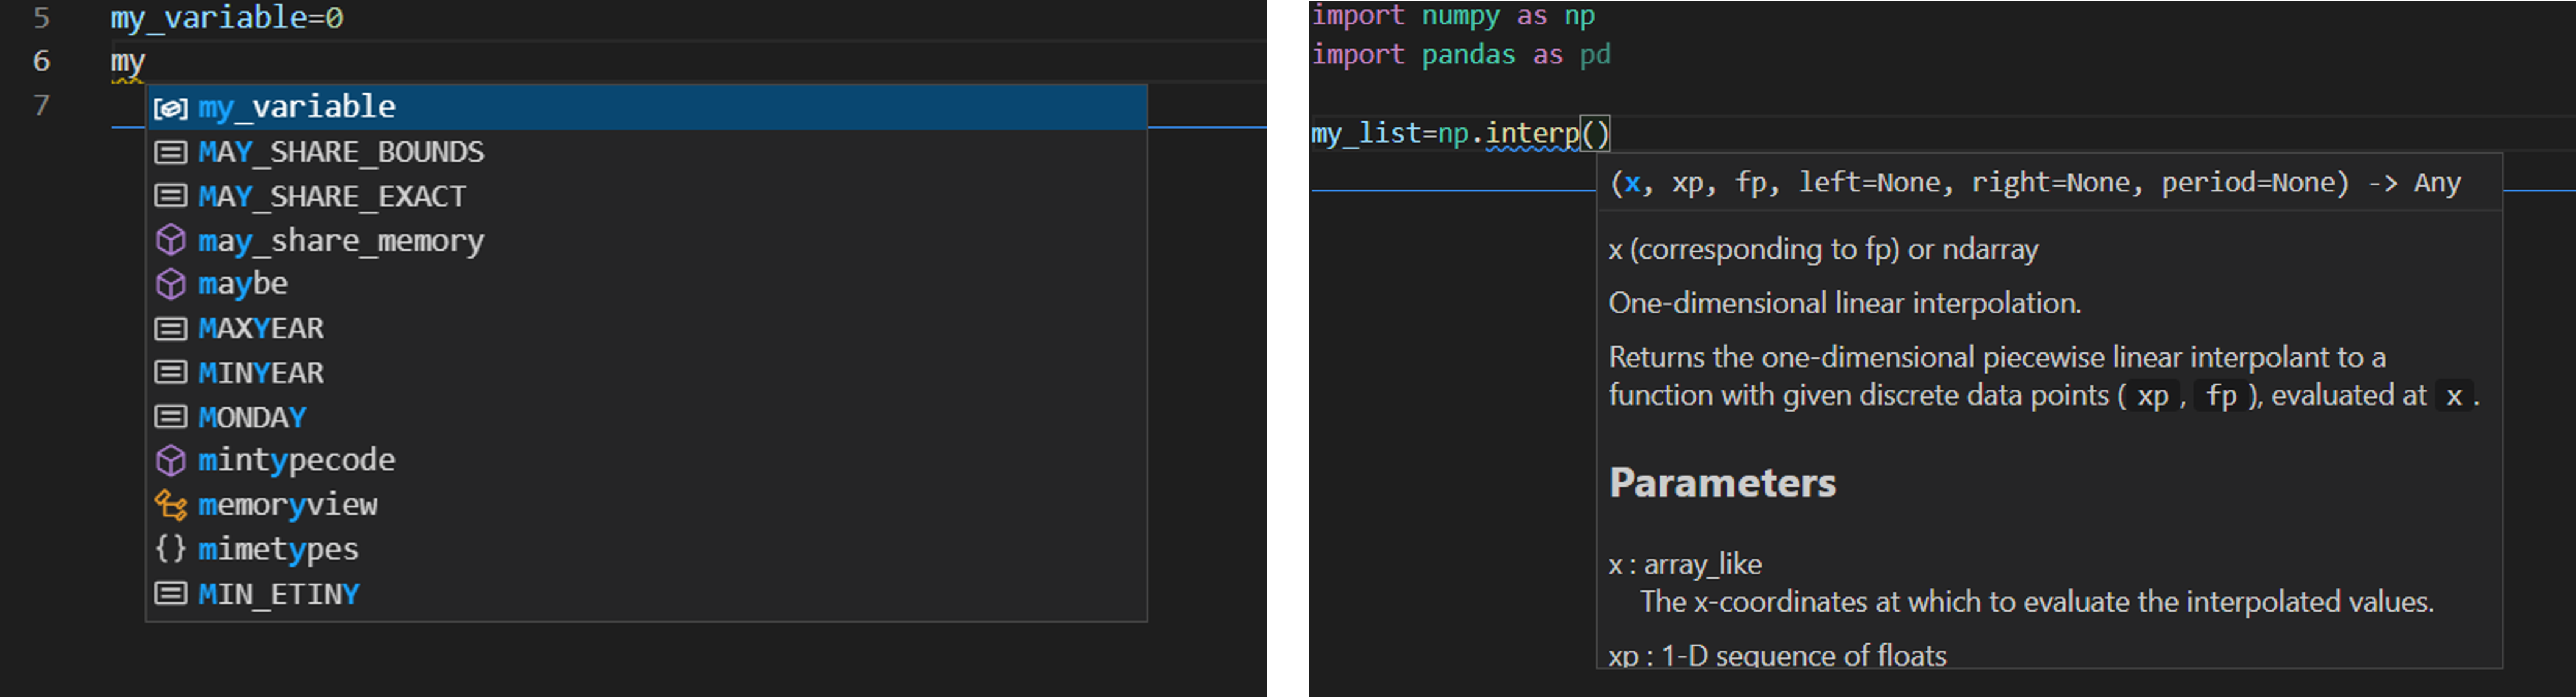
\includegraphics[width=1.0\linewidth]{fig-python/vscode.png}}
  \caption{
  A screenshot of vscode (left) the editor helps to identify which variable name you want, (right) the editor shows relevant information about the function you would like to call. \label{fig:py:vscode}
  }
\end{figure}
%\clearpage % flush figures fig:py:vscode

Currently my favorite editor is \href{{https://code.visualstudio.com/}}{vscode}\footnote{\texttt{https://code.visualstudio.com/}}, it can be used for any language, and there are a lot of add ins that can be installed to make the coding experience more pleasant. Spyder is also a very good alternative, but this editor is mainly for Python. It takes some time to learn how an editor works, so it is good if the editor can be used for multiple purposes.  However, always be open to new ideas and products, it will only make you more efficient. As an example, in some cases you will have a particular difficult error in the code, and then it could help to open and run that code in a different editor, you might get a slightly different error messages, which could help you locate the error.

\section{Types in Python}
\index{types}
In Python you do not need to define types as in a compiled language. In many ways one can say that Python works as if there is only \emph{one} type.  To not define types is generally an advantage as it lets you write code with fewer lines, and it is easier to write functions that will work with any kind of type. As an example, in the programming language C, if you want to write a function that lets you add two numbers, you have to write one version if the arguments are integers and one version if the arguments are floats.

The way that Python store and organize data is called a data model, and it is well described in the \href{{https://docs.python.org/3/reference/datamodel.html}}{official documentation}\footnote{\texttt{https://docs.python.org/3/reference/datamodel.html}}. The important point is that all data in Python is an object or a relation between objects. The \texttt{is} operator can be used to check if two objects have the same identity, that means they are the same object. The \texttt{id} method returns an unique integer value for the object, and if two objects have the same id number they are the same object, e.g.






\begin{lstlisting}[language=python,style=blue1bar]
y=10
x=y
x is y # gives true
print(id(x))
print(id(y)) # prints the same integer as id(x)

\end{lstlisting}

For those familiar with C or C++, one would first have to define \texttt{x} and \texttt{y} as the type \texttt{int} and then they would already have a different place in memory and they can \emph{never} be the same (even if they contain the same number). We will return to this point in more detail when discussing lists and arrays in Python, as it can lead to unexpected behavior.

Another thing you might have experienced during Python coding is that you get error messages that refer to pieces of code that you have no knowledge of. This can happen when you pass the wrong type (e.g.~a string instead of a number). Since Python only has one type, the wrong type will not be discovered before it is actually used. This error could be deep into some other library that you have no knowledge of. 

\subsection{Basic types}
\index{basic types}
I will assume that you are familiar with the common types like floats (for real numbers), strings (text, lines, word, a character), integer (whole numbers), Boolean (True, False). What is sometimes useful is to be able to test what kind of type a variable is, this can be done with the method \texttt{type()}







\begin{lstlisting}[language=python,style=blue1bar]
my_float = 2.0 
my_int   = 3
my_bool  = True
print(type(my_float))
print(type(my_int))
print(type(my_bool))

\end{lstlisting}

The output of the code above will be \texttt{float, int, bool}. If you want to test the type  of a variable you can do





\begin{lstlisting}[language=python,style=blue1bar]
if isinstance(my_int,int):
    print('My variable is integer')
else:
    print('My variable is not integer')

\end{lstlisting}

Python also has build in support for complex numbers. An example are \texttt{1+2j}, \texttt{j} is the imaginary part of the complex number. Note there is no multiplication sign between 2 and \texttt{j}.

\subsection{Lists}

\index{lists} \index{list comprehension}
Lists are extremely useful, and they have very nice syntax that in my opinion is more elegant than Numpy arrays. Whenever you want to do more than one thing with only a slight change between the elements, you should think of lists. Lists are defined using the square bracket \texttt{[]} symbol






\begin{lstlisting}[language=python,style=blue1bar]
my_list = []      # an empty list
my_list = []*10   # still an empty list ...
my_list = [0]*10  # a list with 10 zeros
my_list = ['one', 'two','three'] # a list of strings
my_list = ['one']*10 # a list with 10 equal string elements 

\end{lstlisting}



\begin{graybox2admon}[Notice]
To get the first element in a list, we do e.g. \Verb!my_list[0]!. In a list with 10 elements the last element would be \Verb!my_list[9]!. The length of a list can be found by using the \texttt{len()} function, i.e. \Verb!len(my_list)=10!. Thus, the last element can also be found by doing \Verb!my_list[len(my_list)-1]!. However, in Python you can always get the last element by doing \Verb!my_list[-1]!, the second last element would be \Verb!my_list[-2]! and so on.
\end{graybox2admon}



Sometimes you do not want to initialize the list with everything equal, and it can be tiresome to write everything out yourself. If that is the case you can use \emph{list comprehension}



\begin{lstlisting}[language=python,style=blue1bar]
my_list = [i for i in range(10)] # a list from 0,1,..,9
my_list = [i**3 for i in range(10)] # a list with elements 0,1,8, ..,729

\end{lstlisting}

We will cover the for loop below, but basically what is done is that the statement \texttt{i in range(10)}, gives \texttt{i} the value 0, 1, $\ldots$, 9 and the first \texttt{i} inside the list tells python to use that value as the element in the list. Using this syntax, there are plenty of opportunities to initialize. Maybe you want to pick from a list words that contain a particular subset of characters



\begin{lstlisting}[language=python,style=blue1bar]
my_list  = ['hammer', 'nail','saw','lipstick','shirt']
new_list = [i for i in my_list if 'a' in i]

\end{lstlisting}

Now \Verb!new_list=['hammer', 'nail', 'saw']!.

\paragraph{List arithmetic.}
I showed you some examples above, where we used multiplication to create a list with equal copies of a single element, you can also join two lists by using addition




\begin{lstlisting}[language=python,style=blue1bar]
my_list  = ['hammer','saw']
my_list2 = ['screw','nail','glue']
new_list = my_list + my_list2

\end{lstlisting}

Now \Verb!new_list=['hammer', 'saw', 'screw', 'nail', 'glue']!, we can also multiply the list with an integer and get a larger list with several copies of the original list.

\paragraph{List slicing.}
Clearly we can access elements in a list by using the index to the element, i.e.~first element is \Verb!my_list[0]!, and the last element is \Verb!my_list[-1]!. Python also has very nice syntax to pick out a subset of a list. The syntax is \Verb!my_list[start:stop:step]!, the step makes it possible to skip elements









\begin{lstlisting}[language=python,style=blue1bar]
my_list=['hammer', 'saw', 'screw', 'nail', 'glue']
my_list[:]      # ['hammer', 'saw', 'screw', 'nail', 'glue']
my_list[1:]     # ['saw', 'screw', 'nail', 'glue']
my_list[:-1]    # ['hammer', 'saw', 'screw', 'nail']
my_list[1:-1]   # ['saw', 'screw', 'nail']
my_list[1:-1:2] # ['saw','nail']
my_list[::1]    # ['hammer', 'saw', 'screw', 'nail', 'glue']
my_list[::2]    # ['hammer', 'screw', 'glue']

\end{lstlisting}


Sometimes you have lists of lists, if you want to get e.g.~the first element of each list you cannot access those elements using list slicing, you have to use a for loop or list comprehension






\begin{lstlisting}[language=python,style=blue1bar]
my_list  = ['hammer','saw']
my_list2 = ['screw','nail','glue']
new_list=[my_list,my_list2]
# extract the first element of each list
new_list2 = [ list[0] for list in new_list]

\end{lstlisting}

\Verb!new_list2=['hammer','screw']!



\begin{graybox2admon}[When to use lists]
Use lists if you have mixed types, and as storage containers. Be careful when you do numerical computation not to mix lists and Numpy arrays. Adding two lists e.g. \texttt{[1,2]+[1,1]}, will give you \texttt{[1,2,1,1]}, whereas adding two Numpy arrays will give you \texttt{[2,3]}.
\end{graybox2admon}




\subsection{Numpy arrays}
Numpy arrays are awesome, and they should be your preferred choice when doing numerical operations. We import Numpy as \texttt{import numpy as np}. These are some examples of initialization





\begin{lstlisting}[language=python,style=blue1bar]
import numpy as np
my_array=np.array([0,1,2,3]) # initialized from list
my_array=np.zeros(10) # array with 10 elements equal to zero
my_array=np.ones(10)  # array with 10 elements equal to one

\end{lstlisting}

A typical use of Numpy arrays is when you want to create equally spaced numbers to evaluate a function, this can be done in (at least) two ways



\begin{lstlisting}[language=python,style=blue1bar]
my_array=np.arange(0,1,0.2) # [0, 0.2, 0.4, 0.6, 0.8]
my_array=np.linspace(0,1,5) # [0., 0.25, 0.5, 0.75, 1.]

\end{lstlisting}

Note that in the second case, the edges of the domain (0,1) are included while in the first case the upper edge is not. 



\begin{graybox2admon}[Do not mix Numpy arrays and lists in functions]
If a function is written to use  Numpy arrays as \emph{arguments}, make sure that it \emph{returns} Numpy arrays. If you have to use a list inside the function to e.g.~store the results of a calculation, convert the list to a Numpy array before returning it by \Verb!np.array(my_list)!.
\end{graybox2admon}




\paragraph{Array slicing.}
You can access elements in Numpy arrays in the same way as lists, the syntax is \Verb!my_array[start,stop,step]!








\begin{lstlisting}[language=python,style=blue1bar]
my_array=np.arange(0,6,1)
my_array[:]      # [0,1,2,3,4,5]
my_array[1:]     # [1,2,3,4,5]
my_array[:-1]    # [0,1,2,3,4]
my_array[1:-1]   # [1,2,3,4]
my_array[1:-1:2] # [1,3]
my_array[::2]    # [0,2,4]

\end{lstlisting}

However, as opposed to lists all the basic mathematical operations addition, subtraction, multiplication are meaningful (\emph{if the arrays have equal length, or shape})






\begin{lstlisting}[language=Python,style=gray]
my_array  = np.array([0,1,2])
my_array2 = np.array([3,4,5])
my_array+my_array2 # [3,5,7]
my_array*my_array2 # [0,4,10]
my_array/my_array2 # [0,.25,.4]

\end{lstlisting}

Note that these operations do what you would expect them to do. If you have arrays of arrays, you can easily access elements in the arrays






\begin{lstlisting}[language=Python,style=gray]
my_array  = np.array([[0,1,2],[3,4,5]]) # shape 2x3 matrix
my_array[0,:] # [0,1,2] First row
my_array[1,:] # [3,4,5] Second row
my_array[:,0] # [0,3] First column
my_array[:,1] # [1,4] Second column

\end{lstlisting}

Not the extra \texttt{[]} in the definition of \Verb!my_array!.  Numpy arrays have a shape property, which makes it very easy to create different matrices. The array \texttt{[0,1,2,3,4,5]} has shape (6,), but we can change the shape to create e.g.~a $2\times3$ matrix




\begin{lstlisting}[language=python,style=blue1bar]
my_array  = np.array([0,1,2,3,4,5])
my_array.shape = (2,3) # [[0,1,2],[3,4,5]] 2 rows and 3 columns
my_array.shape = (3,2) # [[0,1],[2,3],[4,5]] 3 rows and 2 columns

\end{lstlisting}


\subsection{Dictionaries}
If you have not used dictionaries before they might feel unnecessary, but if you get used to them and their syntax, they can make your code much more flexible and easier to expand. You should use dictionaries, when you have data sets that you want to access fast. A very good mental image to have is an excel sheet where data are organized in columns. Each column has a header name, or a \emph{key}. Assume we have the following table



{\small   % for Springer style: small table font and more vspace

\vspace{4mm}

\begin{tabular}{ccc}
\hline
\multicolumn{1}{c}{ A } & \multicolumn{1}{c}{ B } & \multicolumn{1}{c}{ C } \\
\hline
1.0 & 2.0 & 3.0 \\
4.0 & 5.0 &     \\
6.0 & 7.0 &     \\
\hline
\end{tabular}

\vspace{4mm}

}


\noindent
This could be represented as a dictionary as


\begin{lstlisting}[language=python,style=blue1bar]
my_dict={'A':[1.0,4.0,6.0],'B':[2.0,5.0,7.0],'C':[3.0]}

\end{lstlisting}

The syntax is \Verb!{key1:values, key2:values2, ...}!. We access the values in the dictionary by the key i.e. \Verb!print(my_dict['A'])! would print \texttt{[1.0,4.0,6.0]}. If you want to print out all the elements in a dictionary, you can use a for loop (see next section for more details about for loops)



\begin{lstlisting}[language=python,style=blue1bar]
for key in my_dict:
    print(key, my_dict[key])

\end{lstlisting}


\section{Looping}
There are basically two ways of iterating through lists or to do a series of computations, using a for-loop or a while-loop. In most cases a for loop can also be written as a while loops and vice versa. You would typically use a for-loop when you are iterating over a fixed number of elements. A good example is when we are iterating in a numerical computation from time zero to the end time. A while-loop is typically used when we do not know before the run time when to stop, this could be that we are waiting for user input or to reach a certain numerical accuracy in our calculation before proceeding.

\subsection{For loops}
A typical example of a for loop is to loop over a list and do something, and maybe during the execution store the results in a list






\begin{lstlisting}[language=python,style=blue1bar]
numbers=['one','two','three','one','two']
result=[] # has to be declared as empty
for number in numbers:
    if number == 'one':
       result.append(1) 

\end{lstlisting}

The result of this code is \texttt{result=[1, 1]}. The \texttt{number} variable changes during the iteration, and takes the value of each element in the list. Note that I use \texttt{numbers} for the list and \texttt{number} as the iterator, this makes it quite easy to read and understand the code. In many cases you want to have the index, not only the element in the list







\begin{lstlisting}[language=python,style=blue1bar]
numbers  = ['one','two','three','one','two']
numerics = [  1  ,  2  ,   3   , 1   , 2   ]
result=[] # has to be declared as empty
for idx,number in enumerate(numbers):
    if number == 'one':
       result.append(numerics[idx]) 

\end{lstlisting}

The result of this code is \texttt{result=[1, 1]}. In this case the function \texttt{enumerate(numbers)} returns two values: the index, which is stored in \texttt{idx}, and the value of the list element, which is stored in \texttt{number}.

A more elegant way to achieve the same results without using the \texttt{enumerate()} function is to use \texttt{zip}







\begin{lstlisting}[language=python,style=blue1bar]
numbers  = ['one','two','three','one','two']
numerics = [  1  ,  2  ,   3   , 1   , 2   ]
result=[] # has to be declared as empty
for numeric,number in zip(numerics,numbers):
    if number == 'one':
       result.append(numeric) 

\end{lstlisting}

The \texttt{zip} function can be used with several lists of same length.

In many cases you might be in a situation that you want to plot more than one function in a plot. It is then very tempting to copy and paste the previous code, but it is more elegant to use a for loop and lists













\begin{lstlisting}[language=python,style=blue1bar]
import numpy as np
import matplotlib.pyplot as plt
x_val   = np.linspace(0,1,100) # 100 equal spaced points from 0 to 1
y_vals  = [x_val,x_val**2]
labels  = [r'x', r'$x^2$']
cols    = ['r','g']
points  = ['-*','-^']
for y_val,label,col,point in zip(y_vals,labels,cols,points):
    plt.plot(x_val,y_val,point,c=col,label=label)
plt.grid()
plt.legend()
plt.show()

\end{lstlisting}

Output of code is shown in figure~\ref{fig:python:loop}.

\begin{figure}[!ht]  % fig:python:loop
  \centerline{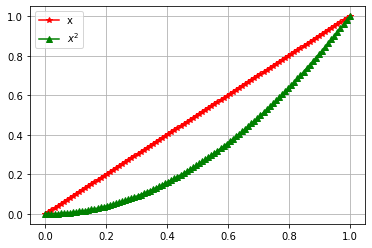
\includegraphics[width=1.0\linewidth]{fig-python/plt_loop.png}}
  \caption{
  Output of code. \label{fig:python:loop}
  }
\end{figure}
%\clearpage % flush figures fig:python:loop

\subsection{While loops}
A while loop is used whenever you do not know before run time when to stop iterating. The syntax of the while loop is to do something while a condition is true








\begin{lstlisting}[language=python,style=blue1bar]
import numpy as np
finished = False
sum =0
while not finished:
      sum += np.random.random() #returns a random number between 0,1
      if sum >= 10.:
      	 finished = True

\end{lstlisting}

In some cases we are iterating from $t_0$, $t_1$, etc. to a final time $t_f$, if we use a fixed time step, $\Delta t$, we can calculate the number of steps i.e $N= \text{int} ((t_f-t_0)/\Delta t)$, and use a for loop. On the other hand, in a more fancy algorithms we can change the time step as the simulation proceeds and then we need to choose a while loop, e.g. \texttt{while t0 <= tf:}. 
\subsection{Functions in Python}
When to use functions? There is no particular rule, \emph{but whenever you
start to copy and paste code from one place to another, you should
consider to use a function}. Functions makes the code easier to read.
It is not easy to identify which part of a program is a good candidate
for a function, it requires skill and experience. Most likely you will
end up changing the function definitions as your program develops.



\begin{graybox2admon}[Use short functions]
Short functions makes the code easier to read. Each function has a particular task, and it does only one thing. If functions do too many tasks there is a chance that you will have several functions doing some of the same operations. Whenever you want to extend the program, you may have to make changes several places in the code. The chance then is that you will forget to do the change in some of the functions and introduce a bug.
\end{graybox2admon}




\subsection{Defining a mathematical function}
Throughout this course you will write many functions that do mathematical operations. In many cases, you would also pass a function to another function to make your code more modular. Lets say we want to calculate the derivative of $\sin x$, using the most basic definition of a derivative $f^\prime(x) = (f(x+\Delta x)-f(x))/\Delta x$, we could do it as






\begin{lstlisting}[language=python,style=blue1bar]
def derivative_of_sine(x,delta_x):
    ''' returns the derivative of sin x '''
    return (np.sin(x+delta_x)-np.sin(x))/delta_x

print('The derivative of sinx at x=0 is :', derivative_of_sine(0,1e-3))

\end{lstlisting}

We will discuss in a later chapter why $\Delta x=10^{-3}$ is a reasonable choice. 
If we would like to calculate the derivative at multiple points, that is straightforward since we have used the Numpy version of $\sin x$.



\begin{lstlisting}[language=python,style=blue1bar]
x=np.array([0,.5,1])
print('Derivative of sinx at x=0,0.5,1 is :', derivative_of_sine(x,1e-3))

\end{lstlisting}

The challenge with our implementation is that if we want to calculate the derivative of another function we have to implement the derivative rule again for that function. It is better to have a separate function that calculates the derivative








\begin{lstlisting}[language=python,style=blue1bar]
def f(x):
    return np.sin(x)

def df(x,f,delta_x=1e-3):
    ''' returns the derivative of f '''
    return (f(x+delta_x)-f(x))/delta_x
print('Derivative of sinx at x=0 is :', df(0,f))

\end{lstlisting}

Note also that we have put \Verb!delta_x=1e-3! as a \emph{default argument}. Default arguments have to come at the end of the argument lists, \Verb!df(x,delta_x=1e-3,f)! is not allowed. All of this looks well, but what you would experience is that your functions would not be as simple as $\sin x$. In many cases your functions need additional arguments to be evaluated e.g.:











\begin{lstlisting}[language=python,style=blue1bar]
def s(t,s0,v0,a):
    '''
    t  : time
    s0 : initial starting point
    v0 : initial velocity
    a  : acceleration
    returns the distance traveled
    '''
    return s0+v0*t+a*t*t*0.5 #multiplication (0.5)is general faster
    	   		     #than division (2)

\end{lstlisting}

How can we calculate the derivative of this function? If we try to do \texttt{df(1,s)} we will get the following message



\begin{lstlisting}[language=python,style=blue1bar]
TypeError: s() missing 3 required positional
	   arguments: 's0', 'v0', and 'a'

\end{lstlisting}

This happens because the \texttt{df} function expect that the function we send into the argument list has a call signature \texttt{f(x)}. What many people do to avoid this error is to use a global variable, that is to define \texttt{s0, v0}, and \texttt{a} at the top of the code. This is not always the best solution. Python has a special variable \texttt{*args} which can be used to pass multiple arguments to your function, thus if we rewrite \texttt{df} like this




\begin{lstlisting}[language=python,style=blue1bar]
def df(x,f,*args,delta_x=1e-3):
    ''' returns the derivative of f '''
    return (f(x+delta_x,*args)-f(x,*args))/delta_x

\end{lstlisting}

we can do (assuming \texttt{s0=0}, \texttt{v0=1}, and \texttt{a=9.8})



\begin{lstlisting}[language=python,style=blue1bar]
print('The derivative of sinx at x=0 is :', df(0,f))
print('The derivative of s(t) at t=1 is :', df(0,s,0,1,9.8))

\end{lstlisting}


\subsection{Scope of variables}
In small programs you would not care about scope, but once you have several functions, you will easily get into trouble if you do not consider the scope of a variable. By scope of a variable we mean where the variable is available, first some simple examples

\paragraph{A variable created inside a function is only available within the function:}
``






\begin{lstlisting}[language=python,style=blue1bar]
def f(x):
    a=10
    b=20
    return a*x+b

\end{lstlisting}

Doing \texttt{print(a)} outside the function will throw an error: \texttt{name 'a' is not defined}. What happens if we define variable \texttt{a} outside the function?






\begin{lstlisting}[language=python,style=blue1bar]
a=2
def f(x):
    a=10
    b=20
    return a*x+b

\end{lstlisting}

If we first call the function \texttt{f(0)}, and then do \texttt{print(a)} Python would give the answer \texttt{2}, \emph{not} \texttt{10}. A \emph{local} variable \texttt{a} is created inside \texttt{f(x)}, that does not interfere with the variable \texttt{a} defined outside the function.

\paragraph{The \texttt{global} keyword can be used to pass and access variables in functions:}

``









\begin{lstlisting}[language=python,style=blue1bar]
global a
a=2
def f(x):
    global a
    a=10
    b=20
    return a*x+b

\end{lstlisting}

In this case \texttt{print(a)} \emph{before} calling \texttt{f(x)} will give the answer \texttt{2} and \emph{after} calling \texttt{f(x)} will give \texttt{10}.



\begin{graybox2admon}[Use of global variables]
Sometimes global variables can be very useful, and help you to make the code simpler. But make sure to use a \emph{naming convention}  for them, e.g.~end all the global variables with an underscore. In the example above we would write \Verb!global a_!. A person reading the code would then know that all variables ending with an underscore are global, and can potentially be modified by several functions.
\end{graybox2admon}




\subsection{Passing arrays and lists to functions}
In the previous section, we looked at some simple examples regarding the scope of variables, and what happened with that variable inside and outside a function. The examples used integer or floats. However in most applications you will pass an array or a list to a function, and then you need to be aware that the behavior is not always what you might expect.


\begin{graybox2admon}[Unexpected behavior]
Sometimes functions do not do what you expect, this might be because the function does not treat  the arguments as you might think. The best advice is to make a very simple version of your function and test it for yourself. Is the behavior what you expect? Try to understand why or why not.
\end{graybox2admon}



Let us look at some examples, and try to understand what is going on and why.








\begin{lstlisting}[language=python,style=blue1bar]
x=3
def f(x):
    x = x*2
    return x
print('x =',x)
print('f(x) returns ', f(x))
print('x is now ', x)

\end{lstlisting}

In the example above we can use \texttt{x=3}, \texttt{x=[3]}, \texttt{x=np.array([3])}, and after execution \texttt{x} is unchanged (i.e.~same value as before \texttt{f(x)}) was called. Based on what we have discussed before, this is maybe what you would expect, but if we now do







\begin{lstlisting}[language=python,style=blue1bar]
x=[3]
def append_to_list(x):
    return x.append(1)
print('x = ',x)
print('append_to_list(x) returns ', append_to_list(x))
print('x is now ', x)

\end{lstlisting}

(Clearly this function will only work for lists, due to the append command.) After execution, we get the result



\begin{lstlisting}[language=python,style=blue1bar]
x = [3]
append_to_list(x) #returns  [3 1], x is now  [3, 1]

\end{lstlisting}

Even if this might be exactly what you wanted your function to do, why does \texttt{x} change here when it is a list and not in the previous case when it is a float? Before we explain this behavior let us rewrite the function to work with Numpy arrays







\begin{lstlisting}[language=python,style=blue1bar]
x=np.array([3])
def append_to_np(x):
    return np.append(x,1)
print('x = ',x)
print('append_to_np(x) returns ', append_to_np(x))
print('x is now ', x)

\end{lstlisting}

The output of this code is



\begin{lstlisting}[language=python,style=blue1bar]
x =  np.array([3])
append_to_np(x) #returns  [3 1], x is now  [3]

\end{lstlisting}

This time \texttt{x} was not changed, what is happening here? It is important to understand what is going on because it deals with how Python handles variables in the memory. If \texttt{x} contains million of values, it can slow down your program, if we do






\begin{lstlisting}[language=python,style=blue1bar]
N=1000000
x=[3]*N
%timeit append_to_list(x)
x=np.array([3]*N)
%timeit append_to_np(x)

\end{lstlisting}

On my computer I found that \Verb!append_to_list! used 76 nano seconds, and \Verb!append_to_np!
used 512 micro seconds, the Numpy function was about 6000 times slower! To add to the confusion consider the following functions
















\begin{lstlisting}[language=python,style=blue1bar]
x=np.array([3])
def add_to_np(x):
    x=x+3
    return x

def add_to_np2(x):
    x+=3
    return x
print('x = ',x)
print('add_to_np(x) returns ', add_to_np(x))
print('x is now ', x)

print('x = ',x)
print('add_to_np2(x) returns ', add_to_np2(x))
print('x is now ', x)

\end{lstlisting}

The output is





\begin{lstlisting}[language=python,style=blue1bar]
x =  np.array([3])
add_to_np(x) #returns [6], x is now [3] 
x =  np.array([3])
add_to_np2(x) #returns  [6], x is now  [6]

\end{lstlisting}

In both cases the function returns what you expect, but it has an unexpected (or at least a different) behavior regarding the variable \texttt{x}. What about speed?






\begin{lstlisting}[language=python,style=blue1bar]
N=10000000
x=np.array([3]*N)
%timeit add_to_np(x)
x=np.array([3]*N)
%timeit add_to_np2(x)

\end{lstlisting}

\Verb!add_to_np! is about twice as slow as \Verb!add_to_np2!. In the next section we will try to explain the difference in behavior.



\begin{graybox2admon}[Avoiding unwanted behavior of functions]
The examples in this section are meant to show you that if you pass an array to a function, the array can be altered outside the scope of the function. If this is not what you want, it could lead to bugs that are hard to detect. Thus, if you experience unwanted behavior pick out the part of function involving list or array operations and test one by one in the editor.
\end{graybox2admon}




\subsection{Call by value or call by reference}
For anyone that has programmed in C or C++ call by reference or value is something one need to think about constantly. When we pass a variable to a function there are two choices, should we pass a copy of the variable or should we pass information about where the variable is stored in memory?


\begin{graybox2admon}[Value and reference]
In C and C++ pass by value means that we are making a copy in the memory of the variable we are sending to the function, and pass by reference means that we are sending the actual parameter or more specific the address to the memory location of the parameter. In Python all variables are passed by object reference.
\end{graybox2admon}



In C and C++ you always tell in the function definition if the variables are passed by value or reference. Thus if you would like a change in a variable outside the function definition, you pass the variable by reference, otherwise by value. In Python we always pass by (object) reference.

\paragraph{Floats and integers.}
To gain a deeper understanding, we can use the \texttt{id} function, the \texttt{id} function gives the unique id to a variable. In C this would be the actual memory address, lets look at a couple of examples





\begin{lstlisting}[language=python,style=blue1bar]
a=10.0
print(id(a)) #gives on my computer 140587667748656
a += 1
print(id(a)) #gives on my computer 140587667748400

\end{lstlisting}

Thus, after adding 1 to \texttt{a}, \texttt{a} is assigned \emph{a new place in memory}. This is very different from C or C++, in C or C++ the variable, once it is created, \emph{always has the same memory address}. In Python this is not the case, it works in the opposite way. The statement \texttt{a=10.0}, is executed so that \emph{first} 10.0 is created in memory, secondly \texttt{a} is assigned the reference to 10.0. The assignment operator \texttt{=} indicates that \texttt{a} should point to whatever is on the right hand side. Another example is     






\begin{lstlisting}[language=python,style=blue1bar]
a=10.0
b=10.0
print(a is b) # prints False
b=a
print(a is b ) # prints True

\end{lstlisting}

In this case 10.0 is created in two different places in the memory and a different reference is assigned to \texttt{a} and \texttt{b}. However if we put \texttt{b=a}, \texttt{b} points to the same object as \texttt{a} is pointing on. More examples






\begin{lstlisting}[language=python,style=blue1bar]
a=10
b=a
print(a is b) # True
a+=2
print(a is b) # False

\end{lstlisting}

When we add 2 to \texttt{a}, we actually add 2 to the value of 10, the number 12 is assigned a new place in memory and \texttt{a} will be assigned that object, whereas \texttt{b} would still points the old object 10.

\paragraph{Lists and arrays.}
Yous should think of lists and arrays as containers (or a box). If we do





\begin{lstlisting}[language=python,style=blue1bar]
x=[0,1,2,3,4]
print(id(x))
x[0]=10
print(id(x)) # same id value as before and x=[10,1,2,3,4]

\end{lstlisting}

First, we create a list, which is basically a box with the numbers 0, 1, 2, 3, 4. The variable \texttt{x} points to \emph{the box}, and \texttt{x[0]} points to 0, and \texttt{x[1]} to 1 etc. Thus if we do \texttt{x[0]=10}, that would be the same as picking 0 out of the box and replacing it with 10, but \emph{the box stays the same}. Thus when we do \texttt{print(x)}, we print the content of the box. If we do







\begin{lstlisting}[language=python,style=blue1bar]
x=[0,1,2,3,4]
y=x
print(x is y) # True
x.append(10)  # x is now [0,1,2,3,4,10]
print(y)      # y=[0,1,2,3,4,10]
print(x is y) # True

\end{lstlisting}

What happens here is that we create a box with the numbers 0, 1, 2, 3, 4, \texttt{x} is referenced to that box. Next, we do \texttt{y=x} so that \texttt{y} is referenced to the \emph{same box} as \texttt{x}. Then, we add the number 10 to that box, and \texttt{x} and \texttt{y} still points to the same box.

Numpy arrays behave differently, and that is basically because if we want to add a number to a Numpy array we have to do \texttt{x=np.array(x,10)}. Because of the assignment operator \texttt{=} , we take the content of the original box add 10 and put it into a \emph{new} box







\begin{lstlisting}[language=python,style=blue1bar]
x=np.array([0,1,2,3,4])
y=x
print(x is y)     # True
x=np.append(x,10) # x is now [0,1,2,3,4,10]
print(y)          # y=[0,1,2,3,4]
print(x is y)     # False

\end{lstlisting}

The reason for this behavior is that the elements in Numpy arrays (contrary to lists) have to be continuous in the memory, and the only way to achieve this is to create a new box that is large enough to also contain the new number. This also explains that if you use the \Verb!np.append(x,some_value)! inside a function where \texttt{x} is large it could slow down your code, because the program has to delete \texttt{x} and create a new very large box each time it would want to add a new element. A better way to do it is to create \texttt{x} \emph{large enough} in the beginning, and then just assign values \texttt{x[i]=a}. 

\subsection{Mutable and immutable objects}
What we have explained in the previous section is related to what is known as mutable and immutable objects. These terms are used to describe objects that have an internal state that can be changed (mutable), and objects that have an internal state that cannot be changed after they have been created. Example of mutable objects are lists, dictionaries, and arrays. Examples of immutable objects are floats, ints, tuples, and strings. Thus if we create the number 10 its value cannot be changed (and why would we do that?). Note that this is \emph{not the same as saying that}  \texttt{x=10} and that the internal state of \texttt{x} cannot change, this is \emph{not} true. We are allowed to make \texttt{x} reference another object. If we do \texttt{x=10}, then \texttt{x is 10} will give true and they will have the same value if we use the \texttt{id} operator on \texttt{x} and \texttt{10}. If we later say that \texttt{a=11} then \texttt{a is 10} will give false and \texttt{id(a)} and \texttt{id(10)} give different values, but * \texttt{id(10)} will have the same value as before*.

Lists are mutable objects, and once a list is created, we can change the content without changing the reference to that object. That is why the operations \texttt{x=[]} and \texttt{x.append(1)}, does not change the id of x, and also explain that if we put \texttt{y=x}, \texttt{y} would change if \texttt{x} is changed. Contrary to immutable objects if \texttt{x=[]}, and \texttt{y=[]} then \texttt{x is y} will give false. Thus, whenever you create a list it will be an unique object.    



\begin{graybox2admon}[A final tip]
You are bound to get into strange, unwanted behavior when working with lists, arrays and dictionaries (mutable) objects in Python. Whenever, you are unsure, just make a simple version of your lists and perform some of the operations on them to investigate if the behavior is what you want.
\end{graybox2admon}



Finally, we show some ``unexpected'' behavior, just to demonstrate that it is easy to do mistakes and one should always test code on simple examples. 






\begin{lstlisting}[language=python,style=blue1bar]
x_old=[]
x  = [1, 2, 3]
x_old[:] = x[:] # x_old = [1, 2, 3]
x[0] = 10
print(x_old) # "expected" x_old = [10, 2, 3], actual [1, 2, 3] 

\end{lstlisting}

Comment: We put the \emph{content} of the \texttt{x} container into \Verb!x_old!, but \texttt{x} and \Verb!x_old! reference different containers.  








\begin{lstlisting}[language=python,style=blue1bar]
def add_to_list(x,add_to=[])
    add_to.append(x)
    return add_to

print(add_to_list(1)) # "expected" [1] actual [1]
print(add_to_list(2)) # "expected" [2] actual [1, 2]
print(add_to_list(3)) # "expected" [3] actual [1, 2, 3]

\end{lstlisting}

Comment: \Verb!add_to=[]! is a default argument and it is created once when the program starts and not each time the function is called.










\begin{lstlisting}[language=python,style=blue1bar]
x = [10]
y = x
y = y + [1]
print(x, y) # prints [10] [10, 1]

x = [10]
y = x
y += [1] 
print(x, y) # prints [10, 1] [10, 1]

\end{lstlisting}

Comment: In the first case \texttt{y + [1]} creates a new object and the assignment operator \texttt{=} assign \texttt{y} to that object, thus \texttt{x} stays the same. In the second case the \texttt{+=} adds \texttt{[1]} to the \texttt{y} container without changing the container, and thus \texttt{x} also changes.

\chapter{Introduction to Pandas}
\label{ch:pan}

\section{What is Pandas?}
Pandas is a Python package that among many things is used to handle data, and perform operations on groups of data. It is built on top of Numpy, which makes it easy to perform vectorized operations. Pandas is written by Wes McKinney, and one of it objectives is according to the official website \href{{https://pandas.pydata.org/}}{'' providing fast, flexible, and expressive data structures designed to make working with ''relational'' or ''labeled'' data both easy and intuitive. It aims to be the fundamental high-level building block for doing practical, real-world data analysis in Python''}\footnote{\texttt{https://pandas.pydata.org/}}. Pandas also has excellent functions for reading and writing excel and csv files.  An excel file is read directly into memory in what is called a \texttt{DataFrame}. A DataFrame is a two dimensional object where data are typically stored in column or row format. Pandas has a lot of functions that can be used to calculate statistical properties of the data frame as a whole. In this chapter, we will focus on basic data manipulation, stuff you might do in excel, but can be done much faster in Python and Pandas.

\section{Creating a data frame}
In the following we will assume that you have imported pandas, like this:


\begin{lstlisting}[language=python,style=blue1bar]
import pandas as pd

\end{lstlisting}


\subsection{From an empty DataFrame}
This is perhaps the most basic way of creating a DataFrame, first we create an empty DataFrame:


\begin{lstlisting}[language=python,style=blue1bar]
df = pd.DataFrame()

\end{lstlisting}



\begin{graybox2admon}[Variable name]
Note that we often use \texttt{df} as a variable name for a DataFrame, this is a choice, but it is a good choice as someone else reading the code could infer from a name that \texttt{df} is a DataFrame. If you need more than one DataFrame variable you could use \texttt{df1}, \texttt{df2}, etc. or even better, use a descriptive name, \Verb!df_sales_data!.
\end{graybox2admon}



Next, we can add columns to the DataFrame:






\begin{lstlisting}[language=python,style=blue1bar]
df=pd.DataFrame()
df['ints']=[0,1,2,3]
df['floats']=[4.,5.,6.,7.]
df['tools']=['hammer','saw','rock','nail']
print(df) # to view data frame

\end{lstlisting}

Note that all columns need to have the same size.



\begin{graybox2admon}[\texttt{pd.Series()}]
Even if we initialize the DataFrame column with a list, the command \texttt{type(df['a'])} will tell you that the column in the DataFrame are of type \texttt{pd.Series()}. Thus the fundamental objects in Pandas are of type \texttt{Series}. Series are more flexible, and it is possible to calculate \texttt{df['a']/df['b']}, whereas \texttt{[0,1,2,3]/[4,5,6,7]} is not possible.
\end{graybox2admon}




\subsection{Create DataFrame from dictionary}
A DataFrame can be easily generated from a dictionary. A dictionary is a special data structure, where an unique key is associated with a data type (key:value pair). In this case, the key would be the title of the column, and the value would be the data in the columns.







\begin{lstlisting}[language=python,style=blue1bar]
my_dict={'ints':[0,1,2,3], 'floats':[4.,5.,6.,7.],
'tools':['hammer','saw','rock','nail']
}
df=pd.DataFrame(my_dict)
print(df) # to view

\end{lstlisting}


\subsection{From a file}
Assume you have some data organized in excel or in a csv file. The csv file could just be a file with column data, they could be separated by a comma or tab.

\begin{figure}[!ht]  % fig:file
  \centerline{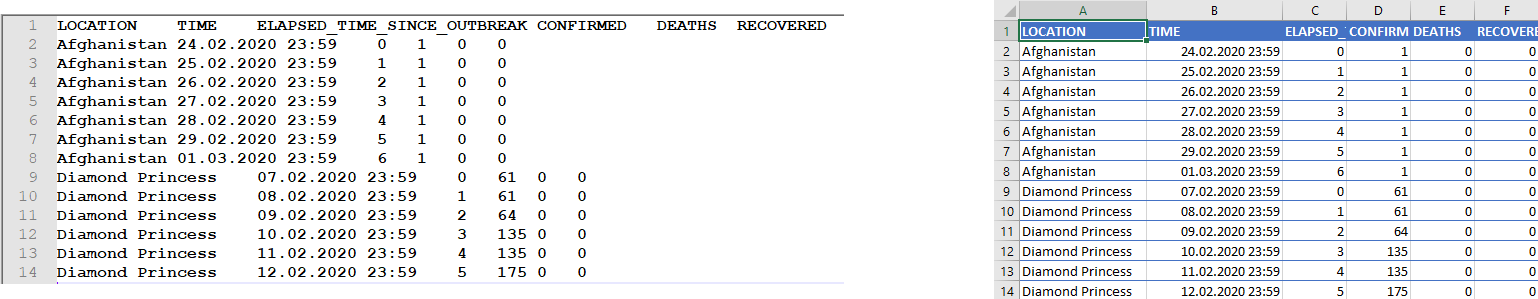
\includegraphics[width=1.0\linewidth]{fig-pandas/covid_comb.png}}
  \caption{
  Official Covid-19 data, and example of files (left) tab separated (right) excel file. \label{fig:file}
  }
\end{figure}
%\clearpage % flush figures fig:file




\begin{lstlisting}[language=python,style=blue1bar]
df=pd.read_excel('../data/corona_data.xlsx') # excel file
df2=pd.read_csv('../data/corona_data.dat',sep='\t') # csv tab separated file

\end{lstlisting}

If the excel file has several sheets, you can give the sheet name directly, e.g. \Verb!df=pd.read_excel('file.xlsx',sheet_name='Sheet1')!, for more information see the \href{{https://pandas.pydata.org/docs/reference/api/pandas.read_excel.html}}{documentation}\footnote{\texttt{https://pandas.pydata.org/docs/reference/api/pandas.read\_excel.html}}. 



\begin{graybox2admon}[Accessing files]
Accessing files from python can be painful. If excel files are open in excel, Windows will not allow a different program to access it - always remember to close the file before opening it. Sometimes we are not in the right directory, to check which directory you are in, you can always do the following



\begin{lstlisting}[language=python,style=blue1bar]
import os
print(os.getcwd()) # prints current working directory

\end{lstlisting}
\end{graybox2admon}




We can easily save the data frame to excel format and open it in Excel


\begin{lstlisting}[language=python,style=blue1bar]
df.to_excel('covid19.xlsx', index=False) # what happens if index=True?

\end{lstlisting}




\begin{graybox2admon}[Index column]
Whenever you create a DataFrame, Pandas by default create an index column, it contains an integer for each row starting at zero. It can be accessed by \texttt{df.index}, and it is also possible to define another column as index column.
\end{graybox2admon}




\subsection{Accessing data in  DataFrames}

\paragraph{Selecting columns.}
If we want to pick out a specific column we can access it in the following way








\begin{lstlisting}[language=python,style=blue1bar]
df=pd.read_excel('../data/corona_data.xlsx') 
# following two are equivalent
time=df['TIME'] # by the name, alternatively
time=df[df.columns[1]]
# following two are equivalent
time=df.loc[:,['TIME']] # by loc[] if we use name
time=df.iloc[:,1] # by iloc, pick column number 1

\end{lstlisting}

The \texttt{loc[]} and \texttt{iloc[]} functions also allow list slicing, one can then pick e.g.~every second element in the column by \texttt{time=df.iloc[::2,1]} etc. The difference is that \texttt{loc[]} uses the name, and \texttt{iloc[]} the index (usually an integer). 

Why do we have several ways of doing the same operation? It turns out that although we are able to extract what we want with these operations, they are of different type:



\begin{lstlisting}[language=python,style=blue1bar]
print(type(df['TIME']))
print(type(df.loc[:,['TIME']]))

\end{lstlisting}

\paragraph{Selecting rows.}
When selecting rows in a DataFrame, we can use the \texttt{loc[]} and \texttt{iloc[]} functions




\begin{lstlisting}[language=python,style=blue1bar]
# pick rows number 0 and 1
time=df.loc[0:1,:] # by loc[] 
time=df.iloc[0:2,:] # by iloc

\end{lstlisting}




\begin{graybox2admon}[\texttt{pandas.DataFrame.loc} vs \texttt{pandas.DataFrame.iloc}]
When selecting rows \texttt{loc} and \texttt{iloc} behave differently, \texttt{loc} includes the endpoints (in the example above both row 0 and 1), whereas \texttt{iloc} includes the starting point and up to the endpoint.
\end{graybox2admon}




\paragraph{Challenges when accessing columns or rows.}


\begin{graybox2admon}[Special characters]
Sometimes when reading files from excel, headers may contains invisible characters like newline \Verb!\n! or tab \Verb!\t! or maybe Norwegian special letters that have not been read in properly. If you have problems accessing a column by name do \texttt{print(df.columns)} and check if the name matches what you would expect.
\end{graybox2admon}




If the header names have unwanted white space, one can do:





\begin{lstlisting}[language=python,style=blue1bar]
df.columns = df.columns.str.replace(' ', '') # all white spaces
df.columns = df.columns.str.lstrip() # the beginning of string
df.columns = df.columns.str.rstrip() # end of string
df.columns = df.columns.str.strip()  # both ends

\end{lstlisting}

Similarly for unwanted tabs:


\begin{lstlisting}[language=python,style=blue1bar]
df.columns = df.columns.str.replace('\t', '') # remove tab

\end{lstlisting}

If you want to make sure that the columns do not contain any white spaces, you can use \href{{https://pandas.pydata.org/pandas-docs/version/1.2.4/reference/api/pandas.Series.str.strip.html}}{\nolinkurl{pandas.Series.str.strip()}\footnote{\texttt{https://pandas.pydata.org/pandas-docs/version/1.2.4/reference/api/pandas.Series.str.strip.html}}}


\begin{lstlisting}[language=python,style=blue1bar]
df['LOCATION']=df['LOCATION'].str.strip()

\end{lstlisting}


\paragraph{Time columns not parsed properly.}
If you have dates in the file (as in our case for the \texttt{TIME} column), you should check if they are in the \texttt{datetime} format and not read as \texttt{str}.



\begin{graybox2admon}[\texttt{datetime}]
The \texttt{datetime} library is very useful for working with dates. Data types of the type \texttt{datetime} (or equivalently \texttt{timestamp} used by Pandas) contain both date and time in the format \texttt{YYYY-MM-DD hh:mm:ss}. We can initialize a variable, \texttt{a}, by \texttt{a=datetime.datetime(2022,8,30,10,14,1)}, to access the hour we do \texttt{a.hour}, the year by \texttt{a.year} etc. It is also easy to increase e.g.~the day by one by doing \texttt{a+datetime.timedelta(days=1)}.
\end{graybox2admon}











\begin{lstlisting}[language=python,style=blue1bar]
import datetime as dt
time=df['TIME']
# what happens if you set
# time=df2['TIME'] #i.e df2 is from pd.read_csv ?
print(time[0])
print(time[0]+dt.timedelta(days=1))

\end{lstlisting}


The code above might work fine or in some cases a date is parsed as a string by Pandas, then we need to convert that column to the correct format. If not, we get into problems if you want to plot data vs the time column.

Below are two ways of converting the \texttt{TIME} column:






\begin{lstlisting}[language=python,style=blue1bar]
df2['TIME']=pd.to_datetime(df2['TIME'])
# just for testing that everything went ok
time=df2['TIME']
print(time[0])
print(time[0]+dt.timedelta(days=1))

\end{lstlisting}


Another possibility is to do the conversion when reading the data:


\begin{lstlisting}[language=python,style=blue1bar]
df2=pd.read_csv('../data/corona_data.dat',sep='\t',parse_dates=['TIME']) 

\end{lstlisting}

If you have a need to specify all data types, to avoid potential problems down the line this can also be done. First create a dictionary, with column names and data types:





\begin{lstlisting}[language=python,style=blue1bar]
types_dict={"LOCATION":str,"TIME":str,"ELAPSED_TIME_SINCE_OUTBREAK":int,
	"CONFIRMED":int,"DEATHS":int,"RECOVERED":int}
df2=pd.read_csv('../data/corona_data.dat',sep='\t',dtype=types_dict,
	parse_dates=['TIME']) # set data types explicit

\end{lstlisting}

Note that the time data type is \texttt{str}, but we explicitly tell Pandas to convert those to \texttt{datetime}.

\subsection{Filtering and visualizing data}
\paragraph{Boolean masking.}
Typically you would select rows based on a criterion, the syntax in Pandas is that you enter a series containing \texttt{True} and \texttt{False} for the rows you want to pick out, e.g.~to pick out all entries with Afghanistan we can do:


\begin{lstlisting}[language=python,style=blue1bar]
df[df['LOCATION'] == 'Afghanistan']

\end{lstlisting}

The innermost statement \texttt{df['LOCATION'] == 'Afghanistan'} gives a logical vector with the value \texttt{True} for the five last elements and \texttt{False} for the rest. Then we pass this to the DataFrame, and in one go the unwanted elements are removed. It is also possible to use several criteria, e.g.~only extracting data after a specific time



\begin{lstlisting}[language=python,style=blue1bar]
df[(df['LOCATION'] == 'Afghanistan') &
		   (df['ELAPSED_TIME_SINCE_OUTBREAK'] > 2)]

\end{lstlisting}

Note that the parenthesis are necessary, otherwise the logical operation would fail.

\paragraph{Plotting a DataFrame.}
Pandas has built in plotting, by calling \href{{https://pandas.pydata.org/docs/reference/api/pandas.DataFrame.plot.html}}{\nolinkurl{pandas.DataFrame.plot}\footnote{\texttt{https://pandas.pydata.org/docs/reference/api/pandas.DataFrame.plot.html}}}.







\begin{lstlisting}[language=python,style=blue1bar]
df2=df[(df['LOCATION'] == 'Afghanistan')]
df2.plot()
#try 
#df2=df2.set_index('TIME')
#df2.plot() # what is the difference?
#df2.plot(y=['CONFIRMED','DEATHS'])

\end{lstlisting}

\subsection{Performing mathematical operations on DataFrames}
When performing mathematical operations on DataFrames there are at least two strategies
\begin{itemize}
\item Extract columns from the DataFrame and perform mathematical operations on the columns using Numpy, leaving the original DataFrame intact

\item To operate directly on the data in the DataFrame using the Pandas library
\end{itemize}

\noindent


\begin{graybox2admon}[Speed and performance]
Using Pandas or Numpy should in principle be equally fast. Do not worry about performance before it is necessary. Use the methods you are confident with, and try to be consistent. By consistent, we mean that if you have found one way of doing a certain operation stick to that one and try not to implement many different ways of doing the same thing.
\end{graybox2admon}




We can always access the individual columns in a DataFrame by the syntax \Verb!df['column_name']!. 
\paragraph{Example: mathematical operations on DataFrames.}
\begin{enumerate}
\item Create a DataFrame with one column (\texttt{a}) containing ten thousand random uniformly distributed numbers between 0 and 1 (checkout \href{{https://numpy.org/doc/stable/reference/random/generated/numpy.random.uniform.html}}{\nolinkurl{np.random.uniform}\footnote{\texttt{https://numpy.org/doc/stable/reference/random/generated/numpy.random.uniform.html}}})

\item Add two new columns: one which all elements of \texttt{a} is squared and one where the sine function is applied to column \texttt{a}

\item Calculate the inverse of all the numbers in the DataFrame

\item Make a plot of the results (i.e. \texttt{a} vs \texttt{a*a}, and \texttt{a} vs \texttt{sin(a)})
\end{enumerate}

\noindent
\paragraph{Solution.}
\begin{enumerate}
\item First we make the DataFrame:
\end{enumerate}

\noindent







\begin{lstlisting}[language=python,style=blue1bar]
import numpy as np
import pandas as pd
N=10000
a=np.random.uniform(0,1,size=N)
df=pd.DataFrame() # empty DataFrame
df['a']=a

\end{lstlisting}

If you like you could also try to use a dictionary. Next, we add the new columns:



\begin{lstlisting}[language=python,style=blue1bar]
df['b']=df['a']*df['a'] # alternatively np.square(df['a'])
df['c']=np.sin(df['a'])

\end{lstlisting}


\begin{enumerate}
\item The inverse of all the numbers in the DataFrame can be calculated by simply doing:
\end{enumerate}

\noindent


\begin{lstlisting}[language=python,style=blue1bar]
1/df

\end{lstlisting}

Note: you can also do \texttt{df+df} and many other operations on the whole DataFrame.

\begin{enumerate}
\item To make plots there are several possibilities. Personally, I tend most of the time to use the  \href{{https://matplotlib.org/}}{\nolinkurl{matplotlib}\footnote{\texttt{https://matplotlib.org/}}} library, simply because I know it quite well, but Pandas has a great deal of very simple methods you can use to generate nice plots with very few commands.
\end{enumerate}

\noindent
\paragraph{Matplotlib:}
``







\begin{lstlisting}[language=python,style=blue1bar]
import matplotlib.pyplot as plt
plt.plot(df['a'],df['b'], '*', label='$a^2$')
plt.plot(df['a'],df['c'], '^', label='$\sin(a)$')
plt.legend() 
plt.grid() # make small grid lines
plt.show()

\end{lstlisting}


\paragraph{Pandas plotting:}
``
First, let us try the built in plot command in Pandas:


\begin{lstlisting}[language=python,style=blue1bar]
df.plot()

\end{lstlisting}

If you compare this plot with the previous plot, you will see that Pandas plots all columns versus the index columns, which is not what we want. But, we can set \texttt{a} to be the index column:



\begin{lstlisting}[language=python,style=blue1bar]
df=df.set_index('a')
df.plot()

\end{lstlisting}

We can also make separate plots:


\begin{lstlisting}[language=python,style=blue1bar]
df.plot(subplots=True)

\end{lstlisting}

or scatter plots




\begin{lstlisting}[language=python,style=blue1bar]
df=df.reset_index()
df.plot.scatter(x='a',y='b')
df.plot.scatter(x='a',y='c')

\end{lstlisting}

Note that we have to reset the index, otherwise there is no column named \texttt{a}. 

\subsection{Grouping, filtering and aggregating data}
Whenever you have a data set, you would like to do some exploratory analysis. That typically means that you would like to group, filter or aggregate data. Perhaps, we would like to plot the covid data not per country, but the data as a function of dates. Then you first must sort the data according to date, and then sum all the occurrences on that particular date. For all of these purposes we can use the \href{{https://pandas.pydata.org/docs/reference/api/pandas.DataFrame.groupby.html}}{\nolinkurl{pd.DataFrame.groupby()}\footnote{\texttt{https://pandas.pydata.org/docs/reference/api/pandas.DataFrame.groupby.html}}} function. To sort our DataFrame on dates and sum the occurrences we can do:



\begin{lstlisting}[language=python,style=blue1bar]
df=pd.read_excel('../data/corona_data.xlsx')
df.groupby('TIME').sum()

\end{lstlisting}


Another case could be that we wanted to find the total number of confirmed, deaths and recovered cases in the full database. As always in Python this can be done in different ways, by e.g.~splitting the database into individual countries and do  \texttt{df[['CONFIRMED','DEATHS','RECOVERED']].sum()} or accessing each column individually and sum each of them e.g. \texttt{np.sum(df['CONFIRMED'])}.  However, with the \texttt{groupby()} function
(see figure~\ref{fig:pandas:group} for final result)


\begin{lstlisting}[language=python,style=blue1bar]
df.groupby('LOCATION').sum()

\end{lstlisting}

Here Pandas sum all columns with the same location, and drop columns that cannot be summed. By doing \texttt{df.groupby('LOCATION').mean()} or \texttt{df.groupby('LOCATION').std()} we can find the mean or standard deviation (per day).

\begin{figure}[!ht]  % fig:pandas:group
  \centerline{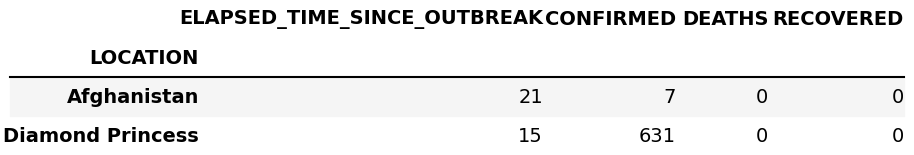
\includegraphics[width=1.0\linewidth]{fig-pandas/group.png}}
  \caption{
  The results of \texttt{df.groupby('LOCATION').sum()}. \label{fig:pandas:group}
  }
\end{figure}
%\clearpage % flush figures fig:pandas:group

\subsection{Simple statistics in Pandas}
Finally, it is worth mentioning the built in methods \texttt{pd.DataFrame.mean}, \texttt{pd.DataFrame.median}, \texttt{pd.DataFrame.std} which calculate the mean, median and standard deviation on the columns in the DataFrame where it make sense (i.e.~avoid strings and dates). To get all these values in one go (and a few more) on can also use \texttt{pd.DataFrame.describe()}


\begin{lstlisting}[language=python,style=blue1bar]
df.describe()

\end{lstlisting}

The output is shown in figure~\ref{fig:pandas:desc}

\begin{figure}[!ht]  % fig:pandas:desc
  \centerline{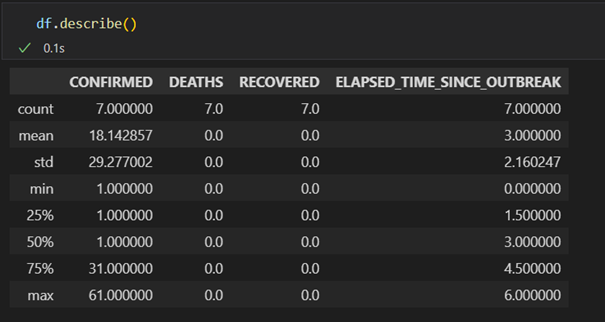
\includegraphics[width=1.0\linewidth]{fig-pandas/describe.png}}
  \caption{
  Output from the describe command. \label{fig:pandas:desc}
  }
\end{figure}
%\clearpage % flush figures fig:pandas:desc

\subsection{Joining two DataFrames}
\paragraph{Appending DataFrames.}
The DataFrame with the Covid-19 data in the previous section could have been created from two separate DataFrames, using \href{{https://pandas.pydata.org/docs/reference/api/pandas.concat.html}}{\nolinkurl{concat()}\footnote{\texttt{https://pandas.pydata.org/docs/reference/api/pandas.concat.html}}}. First, create two DataFrames: 


















\begin{lstlisting}[language=python,style=blue1bar]
import datetime as dt
a=dt.datetime(2020,2,24,23,59)
b=dt.datetime(2020,2,7,23,59)
my_dict1={'LOCATION':7*['Afghanistan'], 
'TIME':[a+dt.timedelta(days=i) for i in range(7)],
'ELAPSED_TIME_SINCE_OUTBREAK':[0, 1, 2, 3, 4, 5, 6],
'CONFIRMED':7*[1],
'DEATHS':7*[0],
'RECOVERED': 7*[0]}
my_dict2={'LOCATION':6*['Diamond Princess'], 
'TIME':[b+dt.timedelta(days=i) for i in range(6)],
'ELAPSED_TIME_SINCE_OUTBREAK':[0, 1, 2, 3, 4, 5],
'CONFIRMED':[61, 61, 64, 135, 135, 175],
'DEATHS':6*[0],
'RECOVERED': 6*[0]}
df1=pd.DataFrame(my_dict1)
df2=pd.DataFrame(my_dict2)

\end{lstlisting}

Next, add them row wise (see figure~\ref{fig:pandas:concat}):




\begin{lstlisting}[language=python,style=blue1bar]
df=pd.concat([df1,df2])
print(df) # to view

\end{lstlisting}


\begin{figure}[!ht]  % fig:pandas:concat
  \centerline{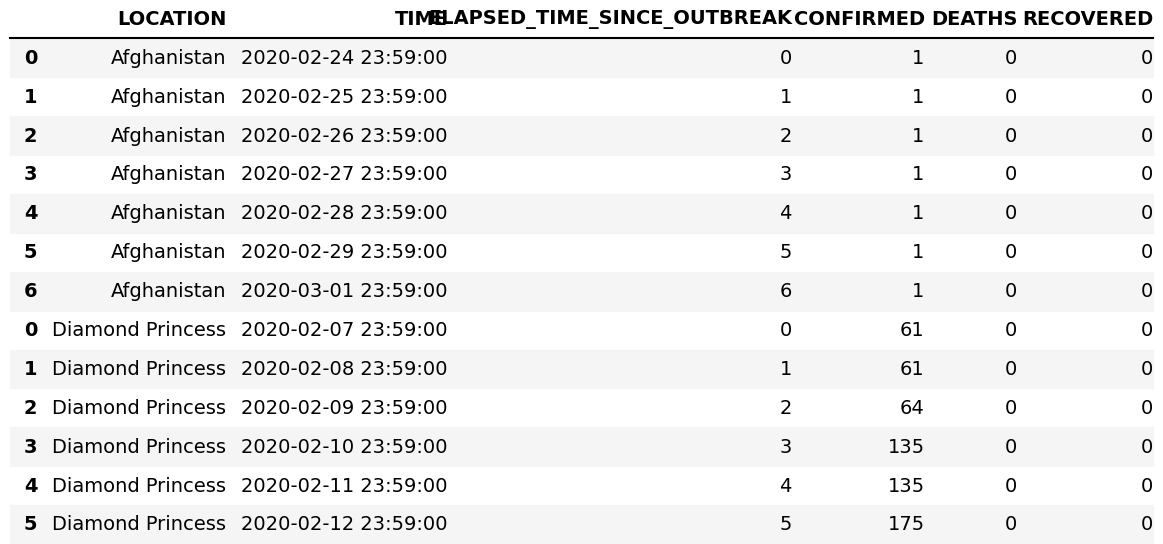
\includegraphics[width=1.0\linewidth]{fig-pandas/concat.png}}
  \caption{
  The result of \texttt{concat()}. \label{fig:pandas:concat}
  }
\end{figure}
%\clearpage % flush figures fig:pandas:concat

If you compare this DataFrame with the previous one, you will see that the index column is different. This is because when joining two DataFrames Pandas does not reset the index by default, doing \Verb!df=pd.concat([df1,df2],ignore_index=True)! resets the index. It is also possible to join DataFrames column wise:


\begin{lstlisting}[language=python,style=blue1bar]
pd.concat([df1,df2],axis=1)

\end{lstlisting}


\paragraph{Merging DataFrames.}
In the previous example we had two non overlapping DataFrames (separate countries and times). It could also be the case that some of the data was overlapping e.g.~continuing with the Covid-19 data, one could assume that there was one data set from one region and one from another region in the same country:















\begin{lstlisting}[language=python,style=blue1bar]
my_dict1={'LOCATION':7*['Diamond Princess'], 
'TIME':[b+dt.timedelta(days=i) for i in range(7)],
'ELAPSED_TIME_SINCE_OUTBREAK':[0, 1, 2, 3, 4, 5, 6],
'CONFIRMED':7*[1],
'DEATHS':7*[0],
'RECOVERED': 7*[0]}
my_dict2={'LOCATION':2*['Diamond Princess'], 
'TIME':[b+dt.timedelta(days=i) for i in range(2)],
'ELAPSED_TIME_SINCE_OUTBREAK':[0, 1],
'CONFIRMED':[60, 60],
'DEATHS':2*[0],
'RECOVERED': 2*[0]}
df1=pd.DataFrame(my_dict1)
df2=pd.DataFrame(my_dict2)

\end{lstlisting}

If we do \texttt{pd.concat([df1,df2])} we will simply add all values after each other. What we want to do is to sum the number of confirmed, recovered and deaths for the same date. This can be done in several ways, but one way is to use \href{{https://pandas.pydata.org/docs/reference/api/pandas.DataFrame.merge.html}}{\nolinkurl{pd.DataFrame.merge()}\footnote{\texttt{https://pandas.pydata.org/docs/reference/api/pandas.DataFrame.merge.html}}}.You can specify the columns to merge on, and choose \texttt{outer} which is union (all data from both frames) or \texttt{inner} which means the intersect (only data which you merge on that exists in both frames), see figure~\ref{fig:pandas:join} for a visual image.

\begin{figure}[!ht]  % fig:pandas:join
  \centerline{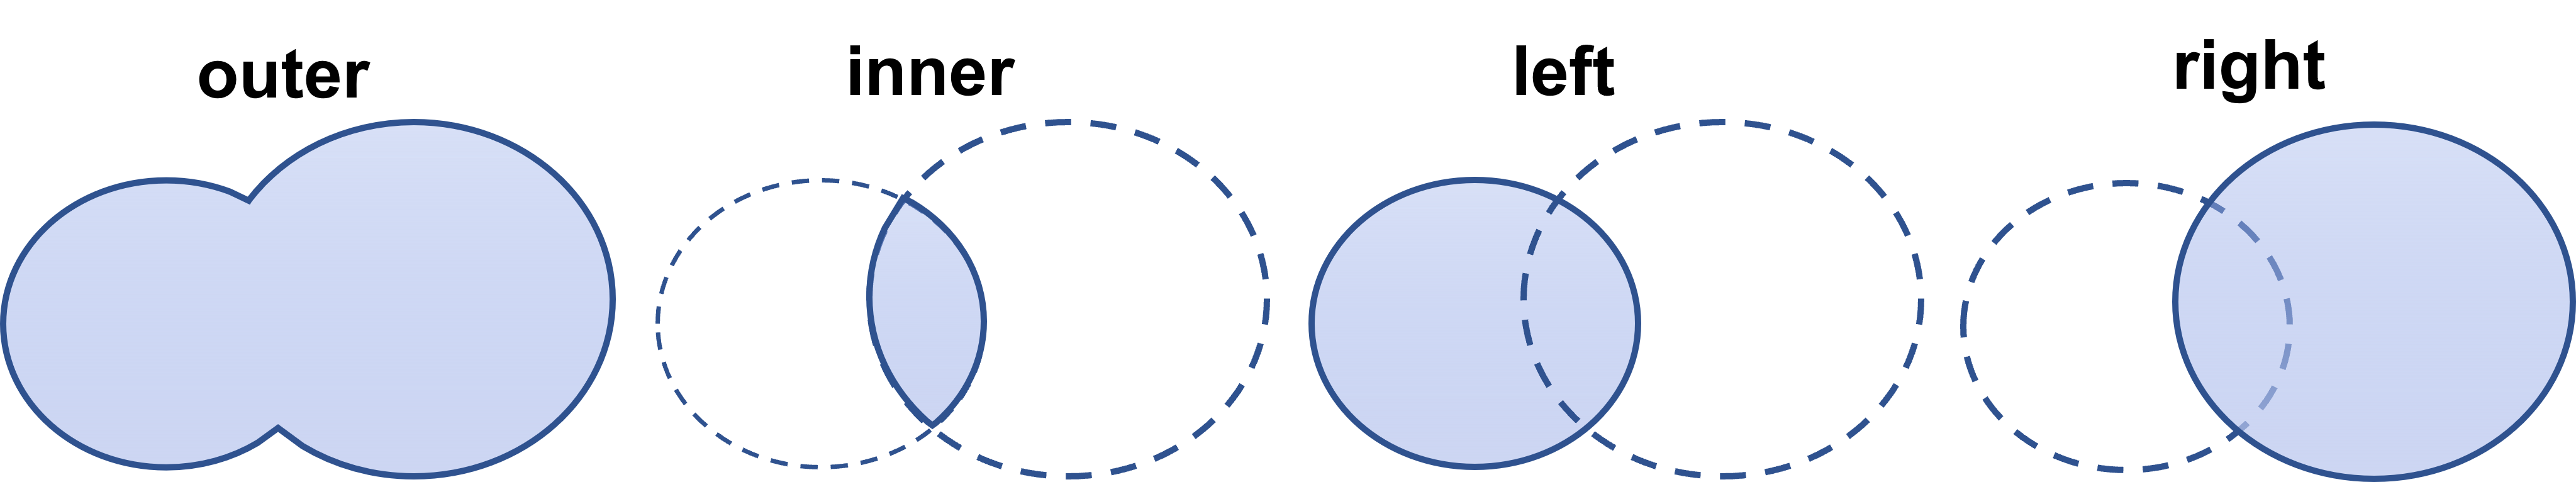
\includegraphics[width=1.0\linewidth]{fig-pandas/fig_join.png}}
  \caption{
  The result of using \texttt{how=outer, inner, left}, or \texttt{right} in \texttt{pd.DataFrame.merge()}. \label{fig:pandas:join}
  }
\end{figure}
%\clearpage % flush figures fig:pandas:join

To be even more specific, after performing the commands



\begin{lstlisting}[language=python,style=blue1bar]
df1.merge(df2,on=['LOCATION','TIME'],how='outer')
df1.merge(df2,on=['LOCATION','TIME'],how='inner')

\end{lstlisting}


we get the results in figure~\ref{fig:pd:merge} 

\begin{figure}[!ht]  % fig:pd:merge
  \centerline{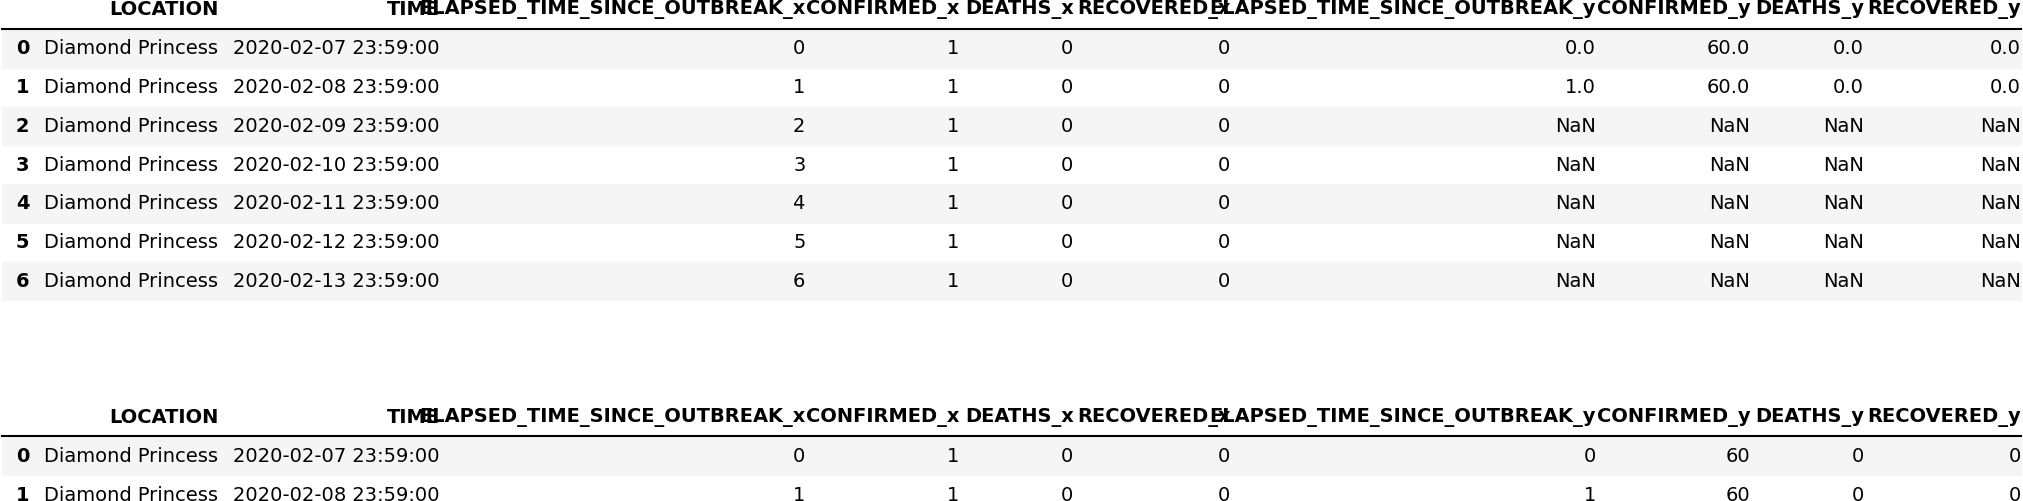
\includegraphics[width=1.0\linewidth]{fig-pandas/merge.png}}
  \caption{
  Merging to dataframes using \texttt{outer} (top) and \texttt{inner} (bottom). \label{fig:pd:merge}
  }
\end{figure}
%\clearpage % flush figures fig:pd:merge

Clearly in this case we need to choose \texttt{outer}. In the merge process pandas adds an extra subscript \Verb!_x! and \Verb!_y! on columns that contain the same header name. We also need to sum those, which can be done as follows
(see figure~\ref{fig:pandas:merge3} for the final result):










\begin{lstlisting}[language=python,style=blue1bar]
df=df1.merge(df2,on=['LOCATION','TIME'],how='outer')
cols=['CONFIRMED','DEATHS', 'RECOVERED']
for col in cols:
    df[col]=df[[col+'_x',col+'_y']].sum(axis=1) # sum row elements
    df=df.drop(columns=[col+'_x',col+'_y']) # remove obsolete columns
# final clean up
df['ELAPSED_TIME_SINCE_OUTBREAK']=df['ELAPSED_TIME_SINCE_OUTBREAK_x']		
df=df.drop(columns=['ELAPSED_TIME_SINCE_OUTBREAK_y','ELAPSED_TIME_SINCE_OUTBREAK_x'])

\end{lstlisting}


\begin{figure}[!ht]  % fig:pandas:merge3
  \centerline{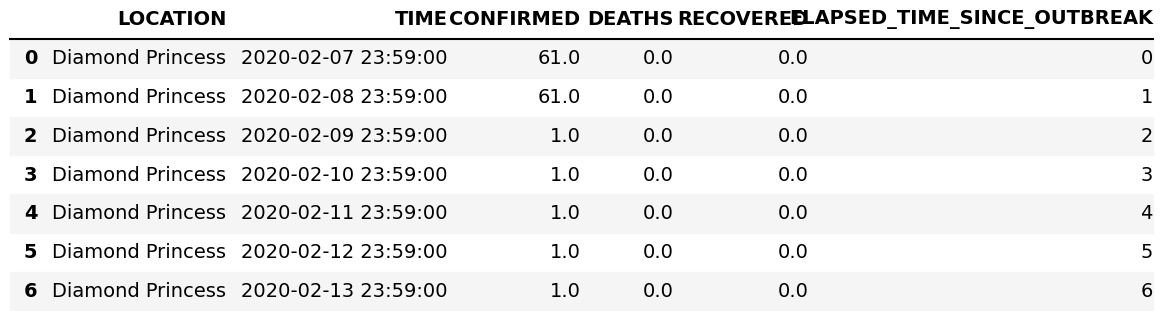
\includegraphics[width=1.0\linewidth]{fig-pandas/merge3.png}}
  \caption{
  Result of outer merging and summing. \label{fig:pandas:merge3}
  }
\end{figure}
%\clearpage % flush figures fig:pandas:merge3

\subsection{Working with folders and files}
When working with big data sets you might want to split data into smaller sets, and also write them to different folders (or files) to view each individually in excel. Working with files and folders in a way that will work on any kind of platform has always been a challenge, but it is greatly simplified by the \href{{https://docs.python.org/3/library/pathlib.html}}{Pathlib library}\footnote{\texttt{https://docs.python.org/3/library/pathlib.html}}.

\paragraph{Basic use of Pathlib.}
\paragraph{List all sub directories and files:}
``








\begin{lstlisting}[language=python,style=blue1bar]
from pathlib import Path
p=Path('.') # the directory where your python file is located
for x in p.iterdir():
    if x.is_dir():
        print('Found dir: ', x)
    elif x.is_file():
        print('Found file: ', x)

\end{lstlisting}


\paragraph{List all files of a type:}
``




\begin{lstlisting}[language=python,style=blue1bar]
p=Path('.')
for p in p.rglob("*.png"):# rglob means recursively, searches sub directories
    print(p.name)

\end{lstlisting}

If you want to print the full path do \texttt{print(p.absolute())}.

\paragraph{Create a directory:}
``


\begin{lstlisting}[language=python,style=blue1bar]
Path('tmp_dir').mkdir()

\end{lstlisting}

If you run the code twice it will produce an error, because the directory exists, then we can simply do \Verb!Path('tmp_dir').mkdir(exist_ok=True)!.

\paragraph{Print current directory:}
``


\begin{lstlisting}[language=python,style=blue1bar]
Path.cwd()

\end{lstlisting}


\paragraph{Joining paths:}
``





\begin{lstlisting}[language=python,style=blue1bar]
p=Path('.')
new_path = p / 'tmp_dir' / 'my_file.txt'
print(new_path.absolute())
new_path.touch()

\end{lstlisting}


\paragraph{Basic use of \texttt{os}.}
We have already encountered the use of \texttt{os} when printing the working directory, i.e. \texttt{print(os.getcwd())}. If you want to create a directory named \texttt{tmp}, one can do

\paragraph{Creating a directory:}
``



\begin{lstlisting}[language=python,style=blue1bar]
import os
os.mkdir('tmp')

\end{lstlisting}

\paragraph{Moving into a directory:}

To move into that directory do`:



\begin{lstlisting}[language=python,style=blue1bar]
os.chdir('tmp')
os.chdir('..') # move back up

\end{lstlisting}


\paragraph{Splitting data into different folders and files.}
\paragraph{Using the Pathlib library:}
``











\begin{lstlisting}[language=python,style=blue1bar]
df=pd.read_excel('../data/corona_data.xlsx')
countries = df['LOCATION'].unique() #skip duplicates
data_folder=Path('../covid-data')
data_folder.mkdir()
for country in countries:
    new_path=data_folder / country
    new_path.mkdir()
    excel_file=country+'.xlsx'
    df2=df[df['LOCATION']==country]
    df2.to_excel(new_path/excel_file,index=False)

\end{lstlisting}

If you run the code twice, it will fail, but that can be resolved by e.g. \Verb!data_folder.mkdir(exist_ok=True)!.  

\paragraph{Using the \texttt{os} library:}
``












\begin{lstlisting}[language=python,style=blue1bar]
# first get all the countries:
df=pd.read_excel('../data/corona_data.xlsx')
countries = df['LOCATION'].unique() #skip duplicates
os.mkdir('../covid-data')
os.chdir('../covid-data')
for country in countries:
    os.mkdir(country)
    os.chdir(country)
    df2=df[df['LOCATION']==country]
    df2.to_excel(country+'.xlsx',index=False)
    os.chdir('..') # move up

\end{lstlisting}


More robust way of creating a directory:







\begin{lstlisting}[language=python,style=blue1bar]
def my_mkdir(name):
    if os.path.isdir(name):
        print('Directory ', name,' already exists')
    else:
        os.mkdir(name)
        print('creating directory ',name)

\end{lstlisting}


If you want to collect all data again, you can do as follows:









\begin{lstlisting}[language=python,style=blue1bar]
df_new=pd.DataFrame()
data_folder=Path('../covid-data')
for dir in data_folder.iterdir():
    if dir.is_dir():      
        file=dir.name+'.xlsx'
        df=pd.read_excel(dir/file)
        print('Reading file ', file)
        df_new=pd.concat([df_new,df],ignore_index=True)

\end{lstlisting}


\subsection{Writing more robust code}
Most likely in the last sections you have encountered long error messages from Python. Errors could be
\begin{itemize}
\item syntax errors, grammatically incorrect code e.g.~calling functions that do not exist, using variables that are not defined or writing lines with missing instructions, indentation errors. 

\item exceptions e.g.~open a file that does not exist, accessing a Pandas header with the wrong name, performing wrong mathematical operations (1/0).

\item logical errors (bugs), code that runs but produces wrong results. These errors are of course some of the most difficult errors to find and can only be discovered by comparing the output of the code to known answers. In many cases errors are introduced when extending the code, and unit tests can be extremely helpful.
\end{itemize}

\noindent
In the rest of this section, we will discuss how to avoid or to handle exceptions. The goal is to write code that catch all the exceptions before they happen, tries to do something with them or prints out a reasonable error message of what went wrong.

Let us look at the code that we have written so far, starting from the top of the notebook.

\paragraph{Accessing columns in Pandas:}
So far we have just accessed the columns directly, but it is very quick to write a wrong name, thus instead of doing


\begin{lstlisting}[language=python,style=blue1bar]
time=df['TIME']

\end{lstlisting}

we should try to check if the column exist before accessing it from the DataFrame. There are many ways of achieving this:
















\begin{lstlisting}[language=python,style=blue1bar]
def get_column_from_dataframe(name,df):
    '''
    name: name of column
    df: Pandas DataFrame
    returns: column if found, and empty otherwise 
    '''
    if name in df.columns:
        return df[name]
    else:
        print('Column not found')
        print('Possible column names are : ', df.columns)
        return pd.Series(dtype=object)
# run the following code with df containing covid data
get_column_from_dataframe('TIME2',df)
get_column_from_dataframe('TIME',df)

\end{lstlisting}

Note the use of doc string in the beginning, the doc string will be printed in advanced editors once you write the name of the function. It also helps you to remember what the function does. It is a good practice to return something of the same type, because then the rest of the code can execute. If it is critical that you find the name of the column, you can always test from the outside:





\begin{lstlisting}[language=python,style=blue1bar]
s=get_column_from_dataframe('TIME2',df)
if s.empty:
    print('Exiting ...')
    exit() # note this shuts down the kernel

\end{lstlisting}

In the function \Verb!get_column_from_dataframe! many more things could go wrong, the user could pass a variable that is not a DataFrame, to catch all exceptions one can do:















\begin{lstlisting}[language=python,style=blue1bar]
def get_column_from_dataframe_v2(name,df):
    '''
    name: name of column
    df: Pandas DataFrame
    returns: column if found, and empty otherwise 
    '''
    try:
        return df[name]
    except:
        print('Something went wrong ...')
        print('Maybe wrong column name?')
        return pd.Series(dtype=object)
# run the following code with df containing covid data
get_column_from_dataframe_v2('TIME2',df)

\end{lstlisting}

The \texttt{try} and \texttt{except} handling is very elegant in Python, and a very easy way of making the code more robust. Python first tries \texttt{df[name]} if that is not successful (e.g.~wrong column name, wrong DataFrame, maybe Pandas is not even imported) it jumps to the exception.

Another thing to consider is case insensitive search, we should be able to access a country or a header using e.g. \texttt{Afghanistan} or \texttt{afghanistan}. A possible solution could be to make sure that when you read in the column, both the DataFrame column and the passed column name are uppercase:


















\begin{lstlisting}[language=python,style=blue1bar]
def get_column_from_dataframe_v3(name,df):
    '''
    name: name of column (case insensitive)
    df: Pandas DataFrame
    returns: column if found, and empty otherwise 
    '''
    COL=df.columns.str.upper()
    NAME=name.upper()
    try:
        idx=COL.get_loc(NAME)
        return df.iloc[:,idx]
    except:
        print('Column not found')
        print('Possible column names are : ', df.columns)
        return pd.Series(dtype=object)
        
get_column_from_dataframe_v3('time',df)

\end{lstlisting}

Now, we might want to make our code more robust by collecting data from specific rows, e.g.~a specific country \texttt{df[df['LOCATION'] == 'Afghanistan']}. This operation assumes 1) that the column \texttt{LOCATION} exists and 2) that the country is spelled correctly. However, we have already written code to get a column and check that it exists, but it is written inside a function with a different purpose. Thus, it is better to split the code above in two parts:










































\begin{lstlisting}[language=python,style=blue1bar]
def get_col_index(name,df):
    '''
    name: name of column (case insensitive)
    df: Pandas DataFrame
    returns: pos if exists, and -1 otherwise 
    '''
    COL=df.columns.str.upper()
    NAME=name.upper()
    try:
        return COL.get_loc(NAME)
    except:
        print('Column not found')
        print('Possible column names are : ', df.columns)
        return -1

def get_column_from_dataframe_v4(name,df):
    '''
    name: name of column (case insensitive)
    df: Pandas DataFrame
    returns: column if found, and empty otherwise 
    '''
    idx=get_col_index(name,df)
    if idx>-1:
        return df.iloc[:,idx]
    else:
        return pd.Series(dtype=object)
        
def get_rows_from_dataframe(name,df,col='LOCATION'):
    '''
    name: name of rows (case insensitive)
    df: Pandas DataFrame
    col: name of column to use as logical test
    returns: DataFrame, and empty otherwise 
    '''
    idx=get_col_index(col,df)
    if idx>-1:
        NAME=name.upper()
        return df[df.iloc[:,idx].str.upper() == NAME]
    else:
        return pd.DataFrame()
get_rows_from_dataframe('afGhaniStan',df)

\end{lstlisting}


\paragraph{To summarize:}

\begin{enumerate}
\item We want to catch errors before they occur, this is most efficiently done by wrapping simple operations in functions.

\item Functions should be as small as possible, that would increase their reusability.

\item Almost all exceptions can be caught by using the \texttt{try} and \texttt{except} functionality in Python

\item Write doc strings in functions to increase user friendliness.

\item Write meaningful error messages, if possible also print out some additional information to help the user.
\end{enumerate}

\noindent
% !split
\chapter{Finite differences}
\label{ch:taylor}

\section{Why are gradients important?}
If you are going to walk up a mountain, it is not enough to know the height of the mountain, you also want to know how steep the mountain is. Even if the mountain is very low, it can still be extremely difficult to reach the top if it is very steep. The steepness is how much the height is changing as a function of time (if we walk with the same pace) or how much the height is changing compared to our horizontal movement. To be more precise lets say we move from $x=a$ to $x=b$, and the height increases from $h_a$ to $h_b$, the steepness is
\begin{equation}
\frac{h_b-h_a}{x_b-x_a}.
\label{eq:tay:gradb}
\end{equation}
If we climb a ladder, the horizontal movement is small ($x_b-x_a$ is small) and the increase in height is large, hence the steepness is large. If we walk a long a flat path we have no vertical movement and the steepness is zero ($h_a=h_b$). Mathematically, if we let $x_b$ and $x_a$ come infinitely close, the steepness is called a \emph{gradient}, and we denote it by $\nabla h(x)$. Note also that the sign of the gradient tells something about the direction. If we climb up a ladder, the height is increasing (positive gradient), on the other hand if we are climbing down the height is decreasing ($h_a>h_b$) and the gradient is negative. 

If we consider the height of a mountain in two dimensions, $h=h(x,y)$, this is basically the contour lines on a map. The spacing between the contour lines is the gradient, if the spacing between contour lines are small the mountain side is steeper than if they are larger.  



\begin{graybox2admon}[Gradients vs derivatives]
If we are only considering a single variable, height as a function of time or position, $x$, we often denote the gradient ($\nabla h$), $h^\prime(x)$ and call it the derivative of $h(x)$. In higher dimension, e.g.~$h(x,y)$, we use the term partial derivatives, because there are now different variables we can vary e.g.~latitude and altitude. The gradient is now a \emph{vector}, $\nabla=[\partial h/\partial x, \partial h/\partial y]$. $\partial h/\partial x$ is the partial derivative of $h(x,y)$ with respect to $x$, i.e.~we keep $y$ constant and only differentiate with respect to $x$.
\end{graybox2admon}




Another example where gradients are important is the flow of heat. Heat flows from hot to cold places, the amount of heat is proportional to the temperature difference, i.e.~a gradient in temperature. The flow of air is also from points of high pressure to low pressure, i.e.~a gradient in pressure. 

A primary task of a modeler is to predict something. If there are no gradients in a system, nothing would happen and there is no reason to model anything. Hence, an extremely important task when we model something is to treat gradients carefully. If gradients are not represented correctly in a computer, the output of a simulation will introduce errors that sometimes can be so large that one cannot trust the simulation results.

\section{Continuous functions and finite representation: numerical errors}
A computer can only deal with numbers. To simulate a physical system in a computer we have to divide space and time into finite pieces, and assign numbers to different parts of time and/or space. 



\begin{graybox2admon}[Numerical errors]
\index{numerical error}
Whenever we divide space and/or time into finite pieces, we introduce numerical errors. These errors tend to become smaller, but not always, when we use more pieces. The difference between the "true" answer and the answer obtained from a practical (numerical) calculation is called the \emph{numerical error}.
\end{graybox2admon}




When we divide space and time into finite pieces to represent them in a computer, a natural question to ask is how many pieces do we need? Consider an almost trivial example, let say you want visualize the function $f(x)=\sin x$. To do this we need to choose where, which values of $x$, we want to evaluate our function. To make an efficient program we want to use as few points as possible but still capture shape of the true function.  
In figure~\ref{fig:taylor:sinx}, we have plotted $\sin x$ for various discretization (spacing between the points) in the interval $[-\pi,\pi]$.

\begin{figure}[!ht]  % fig:taylor:sinx
  \centerline{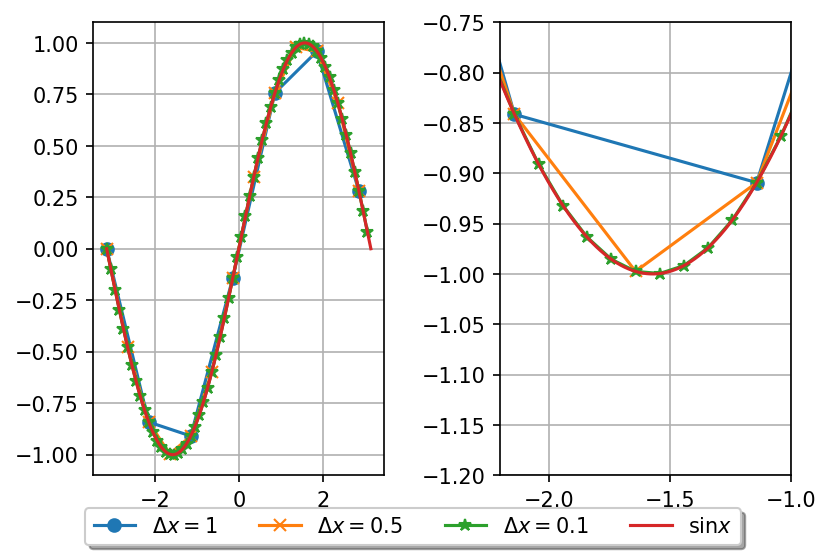
\includegraphics[width=0.9\linewidth]{fig-taylor/func_plot.png}}
  \caption{
  A plot of $\sin x$ for different spacing of the $x$-values. \label{fig:taylor:sinx}
  }
\end{figure}
%\clearpage % flush figures fig:taylor:sinx

From the figure we see that in some areas only a couple of points are needed in order to
represent the function well, and in some areas more points are needed. To state it more clearly; between $[-1,1]$ a linear function (few points) approximate $\sin x$ well, 
whereas in the area where the gradient of the function changes more rapidly e.g.~in $[-2,-1]$, we need the points to be more closely spaced to capture the behavior of the true function.

What is a \emph{good representation} representation of the true function? We cannot rely on visual inspection every time, and most of the time we do not know the true answer so we would not know what to compare it with. In the next section we will show how Taylor polynomial representation of a function is a natural starting point to answer this question.

\section{Taylor polynomial approximation}
How can we evaluate numerical errors if we do not know the true answer? There are at least two answers to this

\begin{enumerate}
\item The pragmatic engineering approach is to do a simulation with a coarse grid, then refine the grid until the solution does not change very much. This is perfectly fine \emph{if you know that your numerical code is bug free}, because even if the simulation converges to a solution we do not know if it is the \emph{true solution}. In too many cases this is not so. Therefore even in well tested industrial codes, it is always good to test them on a simple test case where you know the exact solution.

\item Taylors formula can be used to represent any continuous function with continuous gradients or most solutions to a mathematical model. Taylors formula gives us an estimate of the numerical error introduced when we divide space and time into finite pieces.
\end{enumerate}

\noindent
There are many ways of representing a function, $f(x)$, like Fourier series, Legendre polynomials, but perhaps one of the most widely used is Taylor polynomials.   
Taylor series are perfect for computers, simply because it makes it possible to evaluate any function with a set of limited operations: \emph{addition, subtraction, and multiplication}. Let us start off with the formal definition: 


\begin{graybox2admon}[Taylor polynomial:]
\index{Taylor polynomial}
The Taylor polynomial, $P_n(x)$ of degree $n$ of a function $f(x)$ at the point $c$ is defined as:
\begin{align}
 P_n(x) &= f(c)+f^\prime(c)(x-c)+\frac{f^{\prime\prime}(c)}{2!}(x-c)^2+\cdots+\frac{f^{(n)}(c)}{n!}(x-c)^n\nonumber\\ 
&=\sum_{k=0}^n\frac{f^{(k)}(c)}{k!}(x-c)^k.\label{eq:taylor:taylori}
\end{align}
\end{graybox2admon}



Note that $x$ can be anything, space, time, temperature etc. If the series is around the point $c=0$, the Taylor polynomial $P_n(x)$ is often called a Maclaurin polynomial. If the series converge (i.e.~that the higher order terms approach zero), then we can represent the function $f(x)$ with its corresponding Taylor series around the point $x=c$:
\begin{align}
 f(x) &= f(c)+f^\prime(c)(x-c)+\frac{f^{\prime\prime}(c)}{2!}(x-c)^2+\cdots
=\sum_{k=0}^\infty\frac{f^{(k)}}{k!}(x-c)^k.\label{eq:taylor:taylor}
\end{align}


\begin{graybox2admon}[The magic of Taylors formula]
Taylors formula, equation (\ref{eq:taylor:taylor}), states that if we know the function value and its gradients \emph{in a single point $c$}, we can estimate the function everywhere \emph{using only  information from the single point $c$}. How can this be, how can information in a single point be used to predict the behavior of the function everywhere? One way of thinking about it could be to imagine an object moving in a constant gravitational field without air resistance. Newtons laws then tells us that  if we know the starting point e.g. ($x(0)$), the velocity ($v=dx/dt$), and the acceleration ($a=dv/dt=d^2x/dt^2$) in that point we can predict the trajectory of the object. This trajectory is exactly the first terms in Taylors formula, $x(t)=x(0) + vt+at^2/2$.
\end{graybox2admon}



An example of how Taylors formula works for a known function, can be seen in figure~\ref{fig:mac_sin}, where we show the first nine terms in the Maclaurin series for $\sin x$ (all even terms are zero). 

\begin{figure}[!ht]  % fig:mac_sin
  \centerline{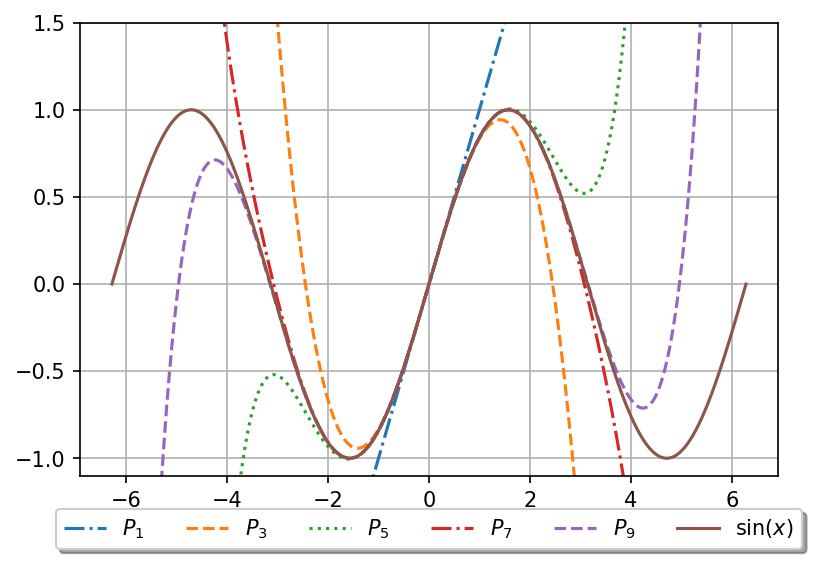
\includegraphics[width=0.9\linewidth]{fig-taylor/mac_sin.png}}
  \caption{
  Nine first terms of the Maclaurin series of $\sin x$. \label{fig:mac_sin}
  }
\end{figure}
%\clearpage % flush figures fig:mac_sin

Notice that close to $x=0$ we only need one term, as we move further away from this point more and more term needs to be added. Thus, Taylors formula is only exact if we include an infinite number of terms. In practice we only include a limited number of terms and truncate the series up to a given order. Luckily, Taylors formula include an estimate of the error we do when we truncate the series. 
\index{truncation error}


\begin{graybox2admon}[Truncation error in Taylors formula:]
\index{Taylor polynomial, error term}
\begin{align}
R_n(x)&=f(x)-P_n(x)=\frac{f^{(n+1)}(\eta)}{(n+1)!}(x-c)^{n+1}\nonumber\\ 
      &=\frac{1}{n!}\int_c^x(x-\tau)^{n}f^{(n+1)}(\tau)d\tau,\label{eq:taylor:error}
\end{align}
Notice that the mathematical formula is basically the next order term ($n+1$) in the Taylor series, but with $f^{(n+1)}(c)\to f^{(n+1)}(\eta)$. $\eta$ is an (unknown) value in the domain $[x,c]$.
\end{graybox2admon}



Notice that if $c$ is very far from $x$ the truncation error increases. The fact that we do not know the value of $\eta$ is usually not a problem, in many cases we just replace $f(\eta)$ with the maximum value it can take on the domain. Equation (\ref{eq:taylor:error}) gives us an direct estimate of discretization error. 


\begin{graybox2admon}[Example: evaluate $\sin x$]
Whenever you do e.g. \texttt{np.sin(1)} in Python or an equivalent statement in another language, Python has to tell the computer how to evaluate $\sin x$ at $x=1$. Write a Python code that calculates $\sin x$ up to a user specified accuracy.

\paragraph{Solution}
The Maclaurin series of $\sin x$ is:
\index{Maclaurin series}
\begin{equation}
\sin x = x-\frac{x^3}{3!}+\frac{x^5}{5!}-\frac{x^7}{7!}+\cdots=\sum_{k=0}^{\infty}\frac{(-1)^n}{(2n+1)!}x^{2n+1}.
\label{sin}
\end{equation}
If we want to calculate $\sin x$ to a precision lower than a specified value we can do it as follows:























\begin{lstlisting}[language=python,style=blue1bar]
import numpy as np

# Sinus implementation using the Maclaurin Serie
# By setting a value for eps this value will be used
# if not provided
def my_sin(x,eps=1e-16):
    f = power = x
    x2 = x*x
    sign = 1
    i=0
    while(power>=eps):
        sign = - sign
        power *= x2/(2*i+2)/(2*i+3)
        f += sign*power
        i += 1
    print('No function evaluations: ', i)
    return f

x=0.8
eps = 1e-9
print(my_sin(x,eps), 'error = ', np.sin(x)-my_sin(x,eps))

\end{lstlisting}


This implementation needs some explanation:

\begin{itemize}
\item The error term is given in equation (\ref{eq:taylor:error}), and it is an even power in $x$. We do not which $\eta$ to use in equation (\ref{eq:taylor:error}), instead we simply say that the error in our estimate is smaller than the highest order term. Thus, we stop the evaluation if the highest order term in the series is lower than the uncertainty. Note that the final error has to be smaller as the higher order terms in any convergent series is smaller than the previous.  Our estimate should then always be better than the specified accuracy.

\item We evaluate the polynomials in the Taylor series by using the previous values too avoid too many multiplications within the loop, we do this by using the following identity:
\end{itemize}

\noindent
  \begin{align}
  \sin x&=\sum_{k=0}^{\infty} (-1)^nt_n, \text{ where: } t_n\equiv\frac{x^{2n+1}}{(2n+1)!}, \text{ hence :}\nonumber\\ 
  t_{n+1}&=\frac{x^{2(n+1)+1}}{(2(n+1)+1)!}=\frac{x^{2n+1}x^2}{(2n+1)! (2n+2)(2n+3)}\nonumber\\ 
  &=t_n\frac{x^2}{(2n+2)(2n+3)}
  \end{align}
\end{graybox2admon}




\section{Calculating Numerical Derivatives of Functions}

As stated earlier many models are described by differential equations. Differential equations contains derivatives, and we need to tell the computer how to calculate those. By using a simple transformation, $x\to x+h$ and $c\to x$ (hence $x-c\to h$), Taylors formula in equation (\ref{eq:taylor:taylor}) can be written
\begin{equation}
f(x+h)=f(x)+f^\prime(x)h+\frac{1}{2}f^{\prime\prime}(x)h^2+\cdots.
\label{eq:taylor:t}
\end{equation}
This is useful because this equation contains the derivative of $f(x)$ on the right hand side. To be even more explicit let us truncate the series to a certain power. Remember that you can always do this but we need to replace $x$ with $\eta$ in the last term we choose to keep
\begin{equation}
f(x+h)=f(x)+f^\prime(x)h+\frac{1}{2}f^{\prime\prime}(\eta)h^2
\label{eq:taylor:t3}
\end{equation}
where $\eta\in[x,x+h]$. Solving this equation with respect to $f^\prime(x)$ gives us
\begin{equation}
f^\prime(x)=\frac{f(x+h)-f(x)}{h}-\frac{1}{2}f^{\prime\prime}(\eta)h.
\label{eq:taylor:fd}
\end{equation}
Note that if $h\to0$, this expression is equal to the definition of the derivative. The beauty of equation (\ref{eq:taylor:fd}) is that it contains an expression for the error we make \emph{when $h$ is not zero}. Equation (\ref{eq:taylor:fd}) is usually called the \emph{forward difference} \index{forward difference}. As you might guess, we can also choose to use the \emph{backward difference} \index{backward difference} by simply replacing $h\to-h$. Is equation (\ref{eq:taylor:fd}) the only formula for the derivative? The answer is no, and we are going to derive the formula for the \emph{central difference} \index{central difference}, by writing Taylors formula for $x+h$ and $x-h$ up to the third order

\begin{align}
f(x+h)&=f(x)+f^\prime(x)h+\frac{1}{2}f^{\prime\prime}(x)h^2+\frac{1}{3!}f^{(3)}(\eta_1)h^3,   
\label{eq:taylor:c1}\\ 
f(x-h)&=f(x)-f^\prime(x)h+\frac{1}{2}f^{\prime\prime}(x)h^2-\frac{1}{3!}f^{(3)}(\eta_2)h^3.
\label{eq:taylor:c2}
\end{align}
where $\eta_1\in[x,x+h]$, and $\eta_2\in[x-h,x]$. Subtracting  equation (\ref{eq:taylor:c1}) and (\ref{eq:taylor:c2}), we get the following expression for the central difference \index{central difference}

\begin{equation}
f^\prime(x)=\frac{f(x+h)-f(x-h)}{2h} -\frac{h^2}{6}f^{(3)}(\eta),\label{eq:taylor:cd}
\end{equation}

where $\eta\in[x-h,x+h]$. Note that the error term in this equation is \emph{one order higher} than in equation (\ref{eq:taylor:fd}), meaning that it is expected to be more accurate. In figure~\ref{fig:taylor:fd} there is a graphical interpretation of the finite difference approximations to the derivative. 

\begin{figure}[!ht]  % fig:taylor:fd
  \centerline{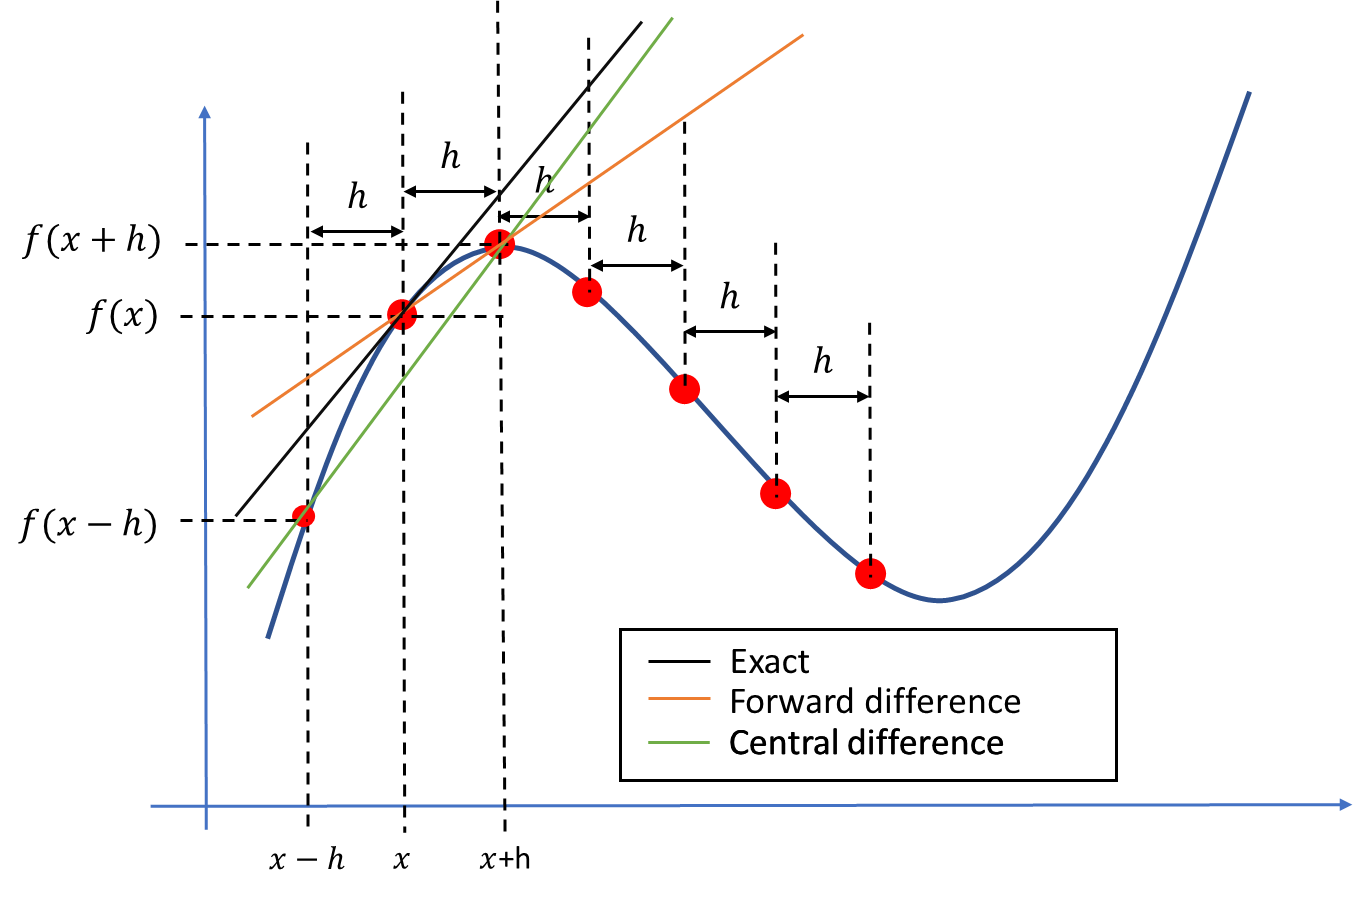
\includegraphics[width=1.0\linewidth]{fig-taylor/fd.png}}
  \caption{
  A graphical interpretation of the forward and central difference formula. \label{fig:taylor:fd}
  }
\end{figure}
%\clearpage % flush figures fig:taylor:fd

\paragraph{Higher order derivative.}
\label{sec:taylor:hhd}
We are also now in the position to derive a formula for the second order derivative. Instead of subtracting equation (\ref{eq:taylor:c1}) and (\ref{eq:taylor:c2}), we can add them. Then the first order derivative disappear and we are left with an expression for the second derivative
\begin{equation}
f^{\prime\prime}(x) = \frac{f(x+h)+f(x-h)-2f(x)}{h^2}- \frac{h^2}{12}f^{(4)}(\eta)
\label{eq:taylor:2der},
\end{equation}
We can also calculate higher order derivatives by expanding about $x\pm h$ and $x\pm 2h$, adding one more term it follows from equation (\ref{eq:taylor:cd})
\begin{align}
f(x+h)-f(x-h)&=2hf^\prime(x)+\frac{2}{3!}h^3f^{(3)}(x)+\frac{2}{5!}h^5f^{(5)}(\eta),\no\\ 
f(x+2h)-f(x-2h)&=2(2h)f^\prime(x)+\frac{2}{3!}(2h)^3f^{(3)}(x)+\frac{2}{5!}h^5f^{(5)}(\eta).
\label{}
\end{align}
It is now possible to find an expression for the third derivative
\begin{equation}
f^{(3)}(x) = \frac{f(x-h)-f(x+h)-\frac{1}{2}f(x-2h)+\frac{1}{2}f(x+2h)}{h^3}+ \frac{h^2}{4}f^{(5)}(\eta)
\label{eq:taylor:3der},
\end{equation}
or a higher order first derivative
\begin{equation}
f^{\prime}(x) = \frac{2f(x+h)-2f(x-h)-\frac{1}{4}f(x+2h)+\frac{1}{4}f(x-2h)}{3h}+ \frac{h^4}{30}f^{(5)}(\eta)
\label{eq:taylor:5der}.
\end{equation}



\begin{graybox2admon}[Example: calculate the numerical derivative and second derivative of $\sin x$]
Choose a specific point, e.g.~$x=1$, and calculate the numerical error for various values of the step size $h$.
\paragraph{Solution:}
The derivative of $\sin x$ is $\cos x$, we can calculate the numerical derivatives using Python






































\begin{lstlisting}[language=python,style=blue1]
def f(x):
    return np.sin(x)
def fd(f,x,h):
    """ f'(x) forward difference """
    return (f(x+h)-f(x))/h

def fc(f,x,h):
    """ f'(x) central difference """
    return 0.5*(f(x+h)-f(x-h))/h

def fdd(f,x,h):
    """ f''(x) second order derivative """
    return (f(x+h)+f(x-h)-2*f(x))/(h*h)

def fd3(f,x,h):
    """ f'''(x) third order derivative """
    return (2*f(x-h)-2*f(x+h)-f(x-2*h)+f(x+2*h))/(2*h*h*h)

def fd_4(f,x,h):
    """ f'(x) fourth order """
    return (8*f(x+h)-8*f(x-h)-f(x+2*h)+f(x-2*h))/(12*h)
x=1
h=np.logspace(-15,0.1,10)
plt.plot(h,np.abs(np.cos(x)-fd(f,x,h)), '-o',label='forward difference')
plt.plot(h,np.abs(np.cos(x)-fc(f,x,h)),'-x', label='central difference')
plt.plot(h,np.abs(np.cos(x)-fd_4(f,x,h)),'-*',label='derivative - fourth order')
plt.plot(h,np.abs(-np.sin(x)-fdd(f,x,h)),'-*',label='second derivative')
h=np.logspace(-7,0.1,10)
plt.plot(h,np.abs(-np.cos(x)-fd3(f,x,h)),'-*',label='third derivative')

plt.grid()
plt.legend()
plt.xscale('log')
plt.yscale('log')
plt.xlabel('Step size $h$')
plt.ylabel('Numerical error')

\end{lstlisting}


In figure~\ref{fig:taylor:df2} you can see the figure produced by the code above.
\end{graybox2admon}




\begin{figure}[!ht]  % fig:taylor:df2
  \centerline{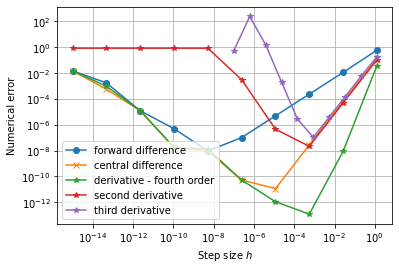
\includegraphics[width=1.0\linewidth]{fig-taylor/df2_mod.png}}
  \caption{
  Numerical error of derivatives of $\sin x$ for various step sizes. \label{fig:taylor:df2}
  }
\end{figure}
%\clearpage % flush figures fig:taylor:df2

There are several important lessons from figure~\ref{fig:taylor:df2}
\begin{enumerate}
\item When the step size is high and decreasing (from right to left in the figure), we clearly see that the numerical error \emph{decreases}.

\item The numerical error scales as expected from right to left. The forward difference formula scales as $h$, i.e.~decreasing the step size by 10 reduces the numerical error by 10. The central difference and second order derivative formula scales as $h^2$, reducing the step size by 10 reduces the numerical error by 100

\item At a certain point the numerical error start to \emph{increase}. For the forward difference formula this happens at $~10^{-8}$.
\end{enumerate}

\noindent
The numerical error has a minimum, \emph{it does not continue to decrease when $h$ decreases}. The explanation for this behavior is two competing effects: \emph{truncation errors} and \emph{roundoff errors}. The truncation errors have already been discussed in great detail, in the next section we will explain roundoff errors.

\subsection{Roundoff Errors}
\index{roundoff erros}
In a computer a floating point number,$x$, is represented as:
\begin{align}
x=\pm q2^m.
\label{eq:taylor:sci2}
\end{align}
This is very similar to our usual scientific notation where we represents large (or small numbers) as $\pm q E m=\pm q 10^{m}$. The processor in a computer handles a chunk of bits at one time, this chunk of bit is usually termed \emph{word}. The number of bits (or byte which almost always means a group of eight bits) in a word is handled as a unit by a processor.   
Most modern computers uses 64-bits (8 bytes) processors. We are not going too much into all the details, the most important message is that the units handled by the processor are \emph{finite}. Thus we cannot, in general, store numbers in a computer with infinite accuracy.


\begin{graybox2admon}[Machine Precision]
\index{machine precision}
Machine precision, $\epsilon_M$ is the smallest number we can add to one and get something different than one, i.e.~$1+\epsilon_M>1$. For a 64-bits computer this value is $\epsilon_M=2^{-52}\simeq2.2210^{-16}$.
\end{graybox2admon}



In the next section we explain exactly why the machine precision has this value, but if you just accept this for a moment we can demonstrate why the machine precision is important and why you need to care about it. First just to convince you that the machine precision has the value of $2^{-52}$ in your computer you can do the following in Python



\begin{lstlisting}[language=python,style=blue1bar]
print(1+2**-52) # prints a value larger than 1
print(1+2**-53) # prints 1.0

\end{lstlisting}

Next, consider the simple calculation




\begin{lstlisting}[language=python,style=blue1bar]
a=0.1+0.2
b=0.3
print(a==b) # gives False

\end{lstlisting}

Why is \texttt{a==b} false, the calculation involves only numbers with one decimal? The reason is that the computer uses the binary system, and in the binary system there is no way of representing 0.2 and 0.3 with a finite number of bits, as an example 0.2 in the binary system is
\begin{equation}
0.2_{10}=0.0011001100\ldots_2 (=2^{-3}+2^{-4}+2^{-7}+2^{-8}+2^{-11}+\cdots)
\label{eq:taylor:02}
\end{equation}
Note that we use the subscript $_{10}$ and $_2$ to represent the decimal and binary system respectively.
Thus in the computer 0.2 will be represented as $0.1999\ldots$ and when we add 0.1 we will get a number really close to 0.3 but not equal to 0.3. Some floats have an exact binary representation e.g.~$0.125_{10}=2^{-8}_{10}=0.00000001_2$. Thus the following code will produce the expected result




\begin{lstlisting}[language=python,style=blue1bar]
a=0.125+0.25
b=0.375
print(a==b) # gives True

\end{lstlisting}



\begin{graybox2admon}[Comparing two floats]
Whenever you want to compare if two floats, $a$ and $b$, are equal in a computer program, you should never do $a==b$ because of roundoff errors. Rather you should choose a variant of $|a-b|<\epsilon$, where you check if the numbers are \emph{close enough}. In practice you also might want to normalize the values and do $|1-b/a|<\epsilon$.
\end{graybox2admon}



The roundoff errors can also play a very big role in calculations, it is particularly apparent when subtracting two numbers of similar magnitude as illustrated in the following code





\begin{lstlisting}[language=python,style=blue1bar]
h=2**-53
a=1+h
b=1-h
print((a-b)/h) # analytical result is 2

\end{lstlisting}

The calculation above is very similar to the calculation done when evaluating derivatives, and if you run the code you will see that Python does not give the expected value of 2.


\begin{graybox2admon}[Choosing the right step size]
A step size that is too low will give higher numerical error because roundoff errors dominate the numerical error.
\end{graybox2admon}



At the end we will mention a simple trick that you can use sometimes to avoid roundoff errors \cite{flannery1992numerical}. In practice we can never get rid of roundoff errors in the calculation $f(x+h)$, but since we can choose the step size $h$ we can choose to choose values such that $x$ and $x+h$ differ by an exact binary number






\begin{lstlisting}[language=python,style=blue1bar]
x=1
h=0.0002 
temp = x+h
h=temp-x
print(h) # improved value of h with exact binary representation

\end{lstlisting}

In the next sections we will show why $\epsilon_M=2^{-52}$, and why a finite word size leads necessary has to imply a maximum and minimum number.  
\paragraph{Binary numbers.}
Binary numbers are used in computers because processors are made of billions of transistors, the end states of a transistor is off or on, representing a 0 or 1 in the binary system. Assume, for simplicity, that we have a processor that uses a word size of 4 bits (instead of 64 bits). How many \emph{unsigned} (positive) integers can we represent in this processor? Lets write down all the possible combinations, of ones and zeros and also do the translation from base 2 numerical system to base 10 numerical system:

\begin{equation}
\begin{matrix}
0&0&0&0=0\cdot 2^3+0\cdot 2^2+0\cdot 2^1+0\cdot 2^0=0\\ 
0&0&0&1=0\cdot 2^3+0\cdot 2^2+0\cdot 2^1+1\cdot 2^0=1\\ 
0&0&1&0=0\cdot 2^3+0\cdot 2^2+1\cdot 2^1+0\cdot 2^0=2\\ 
0&0&1&1=0\cdot 2^3+0\cdot 2^2+1\cdot 2^1+1\cdot 2^0=3\\ 
0&1&0&0=0\cdot 2^3+1\cdot 2^2+0\cdot 2^1+0\cdot 2^0=4\\ 
0&1&0&1=0\cdot 2^3+1\cdot 2^2+0\cdot 2^1+1\cdot 2^0=5\\ 
0&1&1&0=0\cdot 2^3+1\cdot 2^2+1\cdot 2^1+0\cdot 2^0=6\\ 
0&1&1&1=0\cdot 2^3+1\cdot 2^2+1\cdot 2^1+1\cdot 2^0=7\\ 
1&0&0&0=1\cdot 2^3+0\cdot 2^2+0\cdot 2^1+0\cdot 2^0=8\\ 
1&0&0&1=1\cdot 2^3+0\cdot 2^2+0\cdot 2^1+1\cdot 2^0=9\\ 
1&0&1&0=1\cdot 2^3+0\cdot 2^2+1\cdot 2^1+0\cdot 2^0=10\\ 
1&0&1&1=1\cdot 2^3+0\cdot 2^2+1\cdot 2^1+1\cdot 2^0=11\\ 
1&1&0&0=1\cdot 2^3+1\cdot 2^2+0\cdot 2^1+0\cdot 2^0=12\\ 
1&1&0&1=1\cdot 2^3+1\cdot 2^2+0\cdot 2^1+1\cdot 2^0=13\\ 
1&1&1&0=1\cdot 2^3+1\cdot 2^2+1\cdot 2^1+0\cdot 2^0=14\\ 
1&1&1&1=1\cdot 2^3+1\cdot 2^2+1\cdot 2^1+1\cdot 2^0=15
\end{matrix}
.
\label{eq:taylor:bin4}
\end{equation}
Hence, with a 4 bits word size, we can represent $2^4=16$ integers. The largest number is $2^4-1=15$, and the smallest is zero. What about negative numbers? If we still keep to a 4 bits word size, there are still $2^4=16$ numbers, but we distribute them differently. The common way to do it is to reserve the first bit to be a \emph{sign} bit, a "0" is positive and "1" is negative, i.e.~$(-1)^0 = 1$, and $(-1)^1=-1$. Replacing the first bit with a sign bit in equation (\ref{eq:taylor:bin4}), we get the following sequence of numbers 0,1,2,3,4,5,6,7,-0,-1,-2,-3,-4,-5,-6,-7. The "-0", might seem strange but is used in the computer to extend the real number line $1/0=\infty$, whereas $1/-0=-\infty$. In general when there are $m$ bits, we have a total of $2^m$ numbers. If we include negative numbers, we can choose to have $2^{m-1}-1$, negative, and $2^{m-1}-1$ positive numbers, negative zero and positive zero, i.e.~$2^{m-1}-1+2^{m-1}-1+1+1=2^m$.

What about real numbers? As stated earlier we use the scientific notation as in equation (\ref{eq:taylor:sci2}), but still the scientific notation might have a real number in front, e.g.~$1.25\cdot 10^{-3}$. To represent the number $1.25$ in binary format we use a decimal separator, just as with base 10. In this case 1.25 is 1.01 in binary format
\begin{equation}
1.01=1\cdot 2^0 + 0\cdot 2^{-1}+1\cdot 2^{-2}=1 + 0 + 0.25=1.25.
\label{eq:taylor:b2fr}
\end{equation}
The scientific notation is commonly referred to as \emph{floating point representation}. The term "floating point" is used because the decimal point is not in the same place, in contrast to fixed point where the decimal point is always in the same place. To store the number 1e-8=0.00000001 in floating point format, we only need to store 1 and -8 (and possibly the sign), whereas in fixed point format we need to store all 9 numbers.  In equation (\ref{eq:taylor:bin4}) we need to spend one bit to store the sign, leaving (in the case of 4 bits word size) three bits to be distributed among the \emph{mantissa}, $q$, and the exponent, $m$. It is not given how many bits should be used for the mantissa and the exponent. Thus there are choices to be made, and all modern processors uses the same standard, the \href{{https://standards.ieee.org/standard/754-1985.html}}{IEEE Standard 754-1985}\footnote{\texttt{https://standards.ieee.org/standard/754-1985.html}}. 

\paragraph{Floating point numbers and the IEEE 754-1985 standard.}
\index{IEEE 754-1985 standard}
A 64 bits word size is commonly referred to as \emph{double precision}, whereas a 32 bits word size is termed \emph{single precision}. In the following we will consider a 64 bits word size. We would like to know: what is the roundoff error, what is the largest number that can be represented in the computer, and what is the smallest number? Almost all floating point numbers are represented in \emph{normalized} form. In normalized form the mantissa is written as $M=1.F$, and it is only $F$ that is stored,   $F$ is termed the \emph{fraction}. We will return to the special case of some of the unnormalized numbers later. In the IEEE standard one bit is reserved for the sign, 52 for the fraction ($F$) and 11 for the exponent ($m$), see figure~\ref{fig:taylor:64bit} for an illustration.

\begin{figure}[!ht]  % fig:taylor:64bit
  \centerline{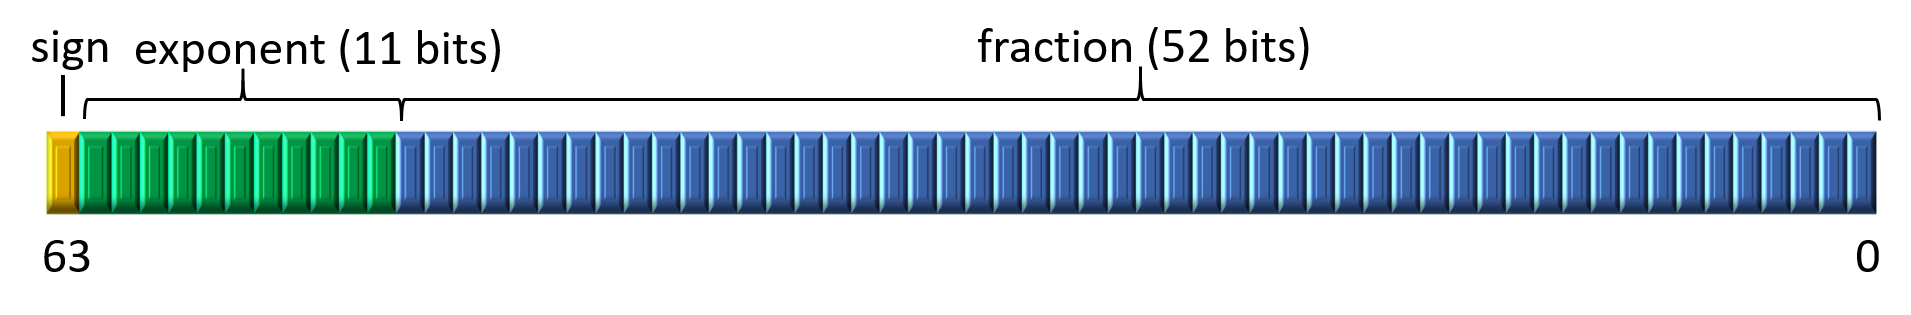
\includegraphics[width=1.0\linewidth]{fig-taylor/64bit.png}}
  \caption{
  Representation of a 64 bits floating point number according to the IEEE 754-1985 standard. For a 32 bits floating point number, 8, is reserved for the exponent and 23 for the fraction. \label{fig:taylor:64bit}
  }
\end{figure}
%\clearpage % flush figures fig:taylor:64bit

The exponent must be positive to represent numbers with absolute value larger than one, and negative to represent numbers with absolute value less than one.  To make this more explicit the simple formula in equation (\ref{eq:taylor:sci2}) is rewritten:
\begin{equation}
\pm q 2^{E-e}.
\label{eq:taylor:ieee}
\end{equation}
The number $e$ is called the \emph{bias} and has a fixed value, for 64 bits it is $2^{11-1}-1=1023$ (32-bits: $e=2^{8-1}-1=127$). The number $E$ is represented by 11 bits and can thus take on values from 0 to $2^11-1=2047$. If we have an exponent of e.g. -3, the computer adds 1023 to that number and store the number 1020. Two numbers are special numbers and reserved to represent infinity and zero, $E=0$ and $E=2047$. Thus \emph{the largest and smallest possible numerical value of the exponent is: 2046-1023=1023, and 1-1023=-1022, respectively}. The fraction of a normalized floating point number takes on values from $1.000\ldots 00$ to $1.111\ldots 11$. Thus the lowest normalized number is
\begin{align}
1.000 + \text{ (49 more zeros)}\cdot 2^{-1022}&=2^0\cdot2^{-1022}\no\\ 
&=2.2250738585072014\cdot 10^{-308}.
\label{}
\end{align}
It is possible to represent smaller numbers than $2.22\cdot10^{-308}$, by allowing \emph{unnormalized} values. If the exponent is -1022, then the mantissa can take on values from $1.000\ldots 00$ to $0.000\ldots 01$, but then accuracy is lost. So the smallest possible number is $2^{-52}\cdot{2^-1022}\simeq4.94\cdot10^{-324}$. 
The highest normalized number is
\begin{align}
1.111 + &\text{ (49 more ones)}\cdot2^{1023}=(2^0+2^{-1}+2^{-2}+\cdots+2^{-52})\cdot2^{1023}\no
\\=(2-2^{-52})\cdot2^{1023}
&=1.7976931348623157\cdot 10^{308}.
\label{}
\end{align}

If you enter \texttt{print(1.8*10**(308))} in Python, the answer will be \texttt{Inf}. If you enter \texttt{print(2*10**(308))}, Python will (normally) give an answer. This is because 
the number $1.8\cdot10^{308}$ is floating point number, whereas $2\cdot 10^{308}$ is an \emph{integer}, and Python does something clever when it comes to representing integers. 
Python has a third numeric type called long int, which can use the available memory to represent an integer.

What about the machine precision? The machine precision, $\epsilon_M$, is the \emph{smallest possible number that can be added to one, and get a number larger than one}, i.e.~$1+\epsilon_M>1$.  The smallest possible value of the mantissa is $0.000\ldots 01=2^{-52}$, thus the lowest number must be of the form $2^{-52}\cdot 2^{m}$. If the exponent , $m$, is lower than 0 then when we add this number to 1, we will only get 1. Thus the machine precision is $\epsilon_M=2^{-52}=2.22\cdot10^{-16}$ (for 32 bits $2^{-23}=1.19\cdot10^{-7}$). In practical terms this means that e.g.~the value of $\pi$ is $3.14159265358979323846264338\ldots$, but in Python it can only be represented by 16 digits: $3.141592653589793$.

\paragraph{Roundoff error and truncation error in numerical derivatives.}


\begin{graybox2admon}[Roundoff Errors]
\index{roundoff errors}
All numerical floating point operations introduces roundoff errors at each step in the calculation due to finite word size, these errors accumulate in long simulations and introduce random errors in the final results. After $N$ operations the error is at least $\sqrt{N}\epsilon_M$ (the square root is a random walk estimate, and we assume that the errors are randomly distributed). The roundoff errors can be much, much higher when numbers of equal magnitude are subtracted. You might be so unlucky that after one operation the answer is completely dominated by roundoff errors.
\end{graybox2admon}




The roundoff error when we represent a floating point number $x$ in the 
machine will be of the order $x/10^{16}$ (\emph{not} $10^{-16}$). In general, when we evaluate a function the error will be of the order 
$\epsilon|f(x)|$, where $\epsilon\sim10^{-16}$. Thus equation (\ref{eq:taylor:fd}) is modified in the following way when we take into account the roundoff errors:
\begin{align}
f^\prime(x)=\frac{f(x+h)-f(x)}{h}\pm\frac{2\epsilon|f(x)|}{h}-\frac{h}{2}f^{\prime\prime}(\eta),\label{eq:taylor:derr2}
\end{align}
we do not know the sign of the roundoff error, so the total error $R_2$ is:
\begin{align}
R_2=\frac{2\epsilon|f(x)|}{h}+\frac{h}{2}|f^{\prime\prime}(\eta)|.\label{eq:taylor:derr3}
\end{align}
We have put absolute values around the function and its derivative to get the maximal error, it might be the case that the roundoff error cancel part of the 
truncation error. However, the roundoff error is random in nature and will change from machine to machine, and each time we run the program. 
Note that the roundoff error increases when $h$ decreases, and the approximation error decreases when $h$ decreases. This is exactly what we saw in figure~\ref{fig:taylor:df2}. We can find the 
best step size, by differentiating $R_2$ and put it equal to zero:
\begin{align}
\frac{dR_2}{dh}&=-\frac{2\epsilon|f(x)|}{h^2}+\frac{1}{2}f^{\prime\prime}(\eta)=0\nonumber\\ 
h&=2\sqrt{\epsilon\left|\frac{f(x)}{f^{\prime\prime}(\eta)}\right|}\simeq 2\cdot10^{-8},\label{eq:taylor:derr4}
\end{align}
In the last equation we have assumed that $f(x)$ and its derivative is $~1$. This step size corresponds to an error of order $R_2\sim10^{-8}$. 
Inspecting figure~\ref{fig:taylor:df2} we see that the minimum is located at $h\sim10^{-8}$.      

We can perform a similar error analysis as we did before, and then we find for equation (\ref{eq:taylor:cd}) and (\ref{eq:taylor:2der}) that the total
numerical error is:
\begin{align}
R_3&=\frac{\epsilon|f(x)|}{h}+\frac{h^2}{6}f^{(3)}(\eta),\label{eq:taylor:derr3b}\\ 
R_4&=\frac{4\epsilon|f(x)|}{h^2}+\frac{h^2}{12}f^{(4)}(\eta),\label{eq:taylor:derr4b}
\end{align}
respectively. Differentiating these two equations with respect to $h$, and set the equations equal to zero, we find an optimal step size of
$h\sim10^{-5}$ for equation (\ref{eq:taylor:derr3b}), which gives an error of $R_2\sim 10^{-16}/10^{-5}+(10^{-5})^2/6\simeq10^{-10}$, and $h\sim10^{-4}$ for equation
(\ref{eq:taylor:derr4b}), which gives an error of $R_4\sim 4\cdot10^{-16}/(10^{-4})^2+(10^{-4})^2/12\simeq10^{-8}$. Note that we get the surprising result for the first order 
derivative in equation (\ref{eq:taylor:cd}), that a higher step size gives a more accurate result. 

% !split

\chapter{Partial differential equations and linear systems}
\label{ch:lin}
Most problems in nature are nonlinear. That means that the system response is not proportional to the system variables, e.g.~doubling the CO$_2$ concentration in the atmosphere does not lead to a doubling of the earth surface temperature. Still, linear solvers lies at the heart of all grid based models describing e.g.~the earths climate. The reason is that although the \emph{global} model is nonlinear, the model can be formulated \emph{locally} as a linear model. Typically the simulation code solves the nonlinear problem through a series of steps where each step is a solution of a linear problem. The topic of solving linear systems of equations have been extensively studied, and sophisticated linear equation solving packages have been developed. Python uses functions from the \href{{https://en.wikipedia.org/wiki/LAPACK}}{LAPACK}\footnote{\texttt{https://en.wikipedia.org/wiki/LAPACK}} library.

In the next sections we will show in detail how differential equations can be solved as a linear problem. We will first start off by deriving one of the most useful differential equations describing conservation of a quantity, e.g.~mass, energy, momentum, charge.

\section{The continuity equation}
\index{continuity equation}
The continuity equation is fundamental to all mathematical models describing a physical phenomenon. To gain more understanding of its origin we will take the time to derive it from first principles. We will do so in one dimension, consider a volume in space between $A(x)$ and $A(x+dx)$ in figure~\ref{fig:lin:flux}. To be concrete we will assume that the green arrows represents the flow of heat. Thus there are heat flowing into and out of the system, and also heat that can be generated within the system by e.g.~chemical reactions. The conservation equation can be formulated with words

\begin{figure}[!ht]  % fig:lin:flux
  \centerline{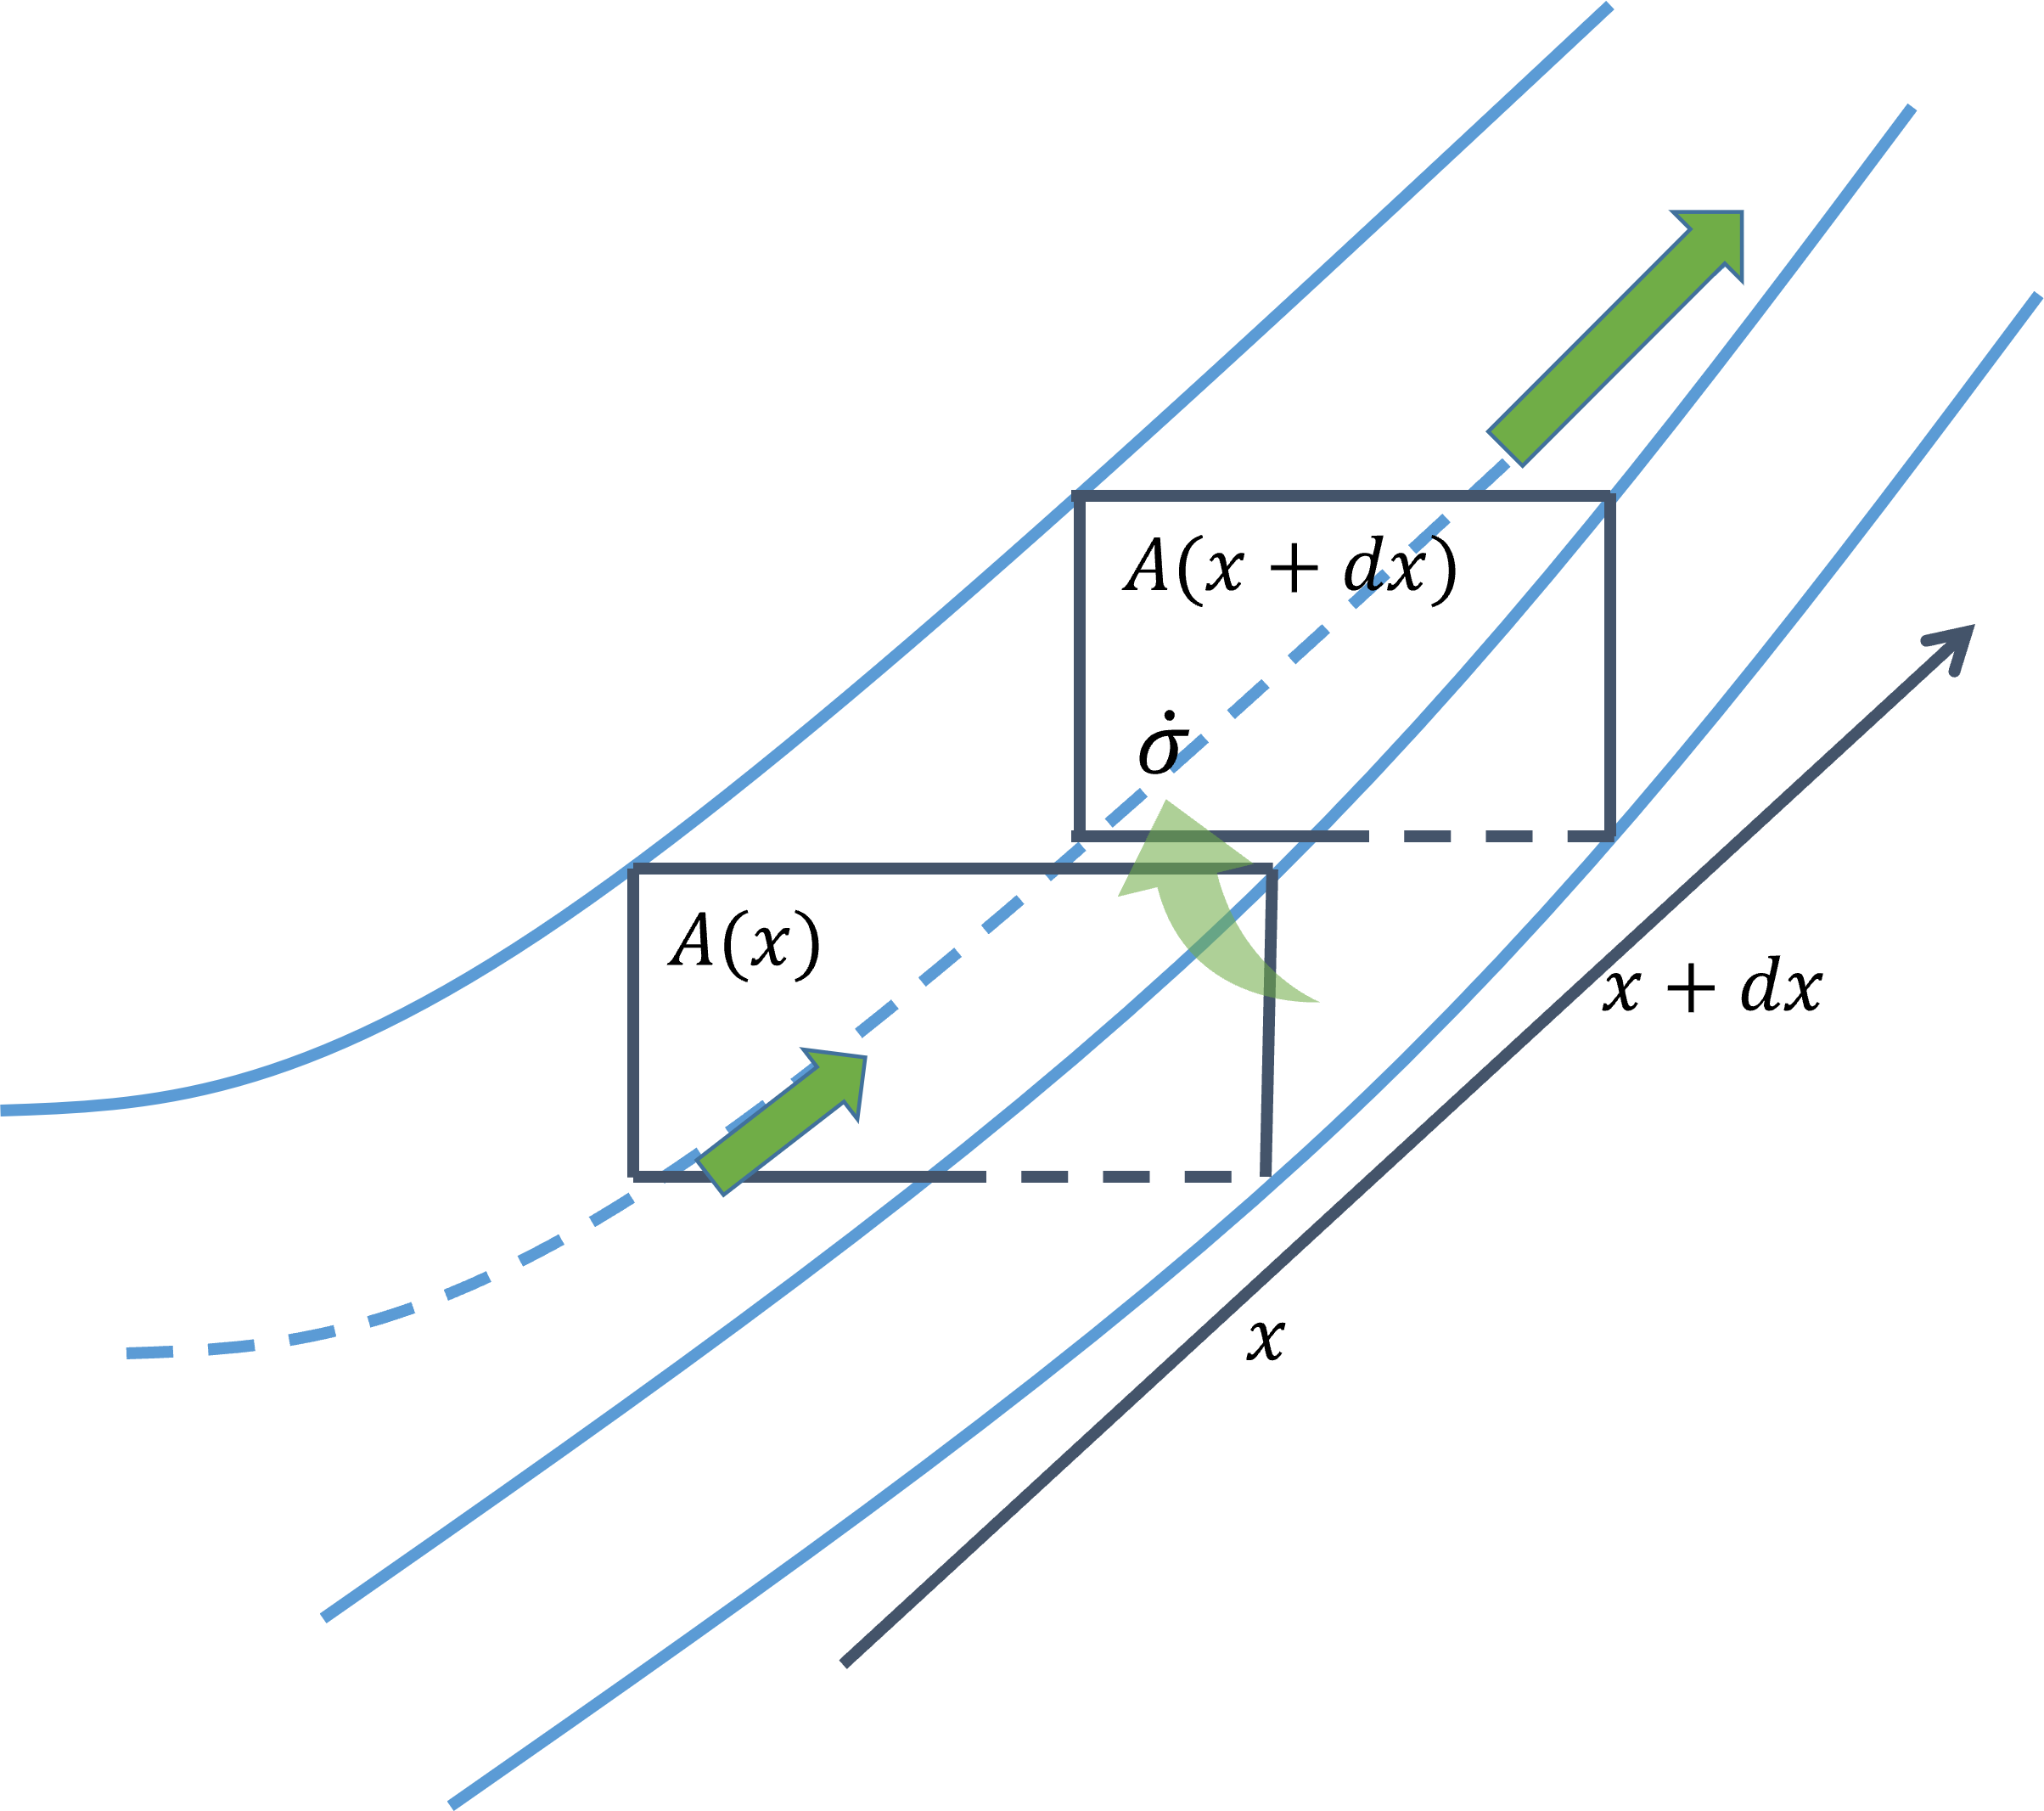
\includegraphics[width=0.5\linewidth]{fig-lin/flux.png}}
  \caption{
  A closed volume, $V(x)=A(x)dx$, where a quantity flows in and out (illustrated by the green lines), there is also a possibility for generation or loss of the same quantity inside the volume. \label{fig:lin:flux}
  }
\end{figure}
%\clearpage % flush figures fig:lin:flux

\begin{align}
\frac{\text{heat into V(x)}}{\text{time}}-\frac{\text{heat out of V(x)}}{\text{time}}
&+\frac{\text{heat generated in V(x)}}{\text{time}} \no\\ 
&= \frac{\text{change of heat in V(x)}}{\text{time}}.
\label{eq:lin:flux}
\end{align}
We formulate the conservation equation per time, because we would like to investigate the time dependency of heat flow. The next step is to replace the terms ''heat into/out of'' with a useful mathematical quantity. It turns out that the term \emph{flux} is particularly useful, because it is an \emph{intensive} quantity. An intensive quantity is a quantity that is \emph{independent of the system size}, like density. The flux is denoted by the symbol $J$
\begin{equation}
J(x)=\frac{\text{quantity (heat)}}{\text{area}\cdot\text{time}},
\label{}
\end{equation}
and was first introduced by Isaac Newton. Thus to find the amount of heat transported through a surface per time we simply multiply the flux with the surface area. Next, we define the heat per volume as $q(x)$, and the heat produced per volume as $\sigma$. Then equation (\ref{eq:lin:flux}) can be written
\begin{align}
\frac{J(x)A(x)}{dt}-\frac{J(x+dx)A(x+dx)}{dt}&+
\frac{\sigma(t+dt)V(x)-\sigma(t)V(x)}{dt}\no\\=
&\frac{q(t+dt)V(x)-q(t)V(x)}{dt}.
\label{eq:lin:cont1}
\end{align}
Using Taylor expansion we can write
\begin{align}
J(x+dx)A(x+dx) &=J(x)A(x)+\frac{d(J(x)A(x)}{dx}dx+{\cal O}(dx^2),
\label{eq:lin:cont2} \\ 
\sigma(t+dt) &=\sigma(t)+\frac{d\sigma}{dt}dt+{\cal O}(dt^2),\no\\ 
q(t+dt) &=q(t)+\frac{dq}{dt}dt+{\cal O}(dt^2),
\label{eq:lin:cont3}
\end{align}
Inserting these equations into equation(\ref{eq:lin:cont1}), using $V(x)=A(x)dx$, and taking the limit $dx,dt\to0$ we arrive at


\begin{graybox2admon}[The continuity equation in 1 dimension]
\begin{equation}
-\frac{d(J(x)A(x))}{dx}+\frac{d\sigma(t)}{dt}A(x)=\frac{dq(t)}{dt}A(x).
\label{eq:lin:cont4}
\end{equation}
\end{graybox2admon}



We have kept the area in equation (\ref{eq:lin:cont4}), because we are only considering flow of heat in one dimension and then we can allow for the area to change in the $y$ and $z$ dimension. When the continuity equation is derived in three dimensions, one consider a volume $V(x,y,z)=dxdydz$, then the area in equation (\ref{eq:lin:cont4}) will drop out and $d/dx\to\nabla=[\partial/\partial x, \partial/\partial y, \partial/\partial z]$ 


\begin{graybox2admon}[The continuity equation in 3 dimensions]
\begin{equation}
-\nabla\cdot\mathbf{J}+\frac{d\sigma(t)}{dt}=\frac{dq(t)}{dt}.
\label{eq:lin:cont5}
\end{equation}
\end{graybox2admon}




\section{Continuity equation as a linear problem}

How can a differential equation be formulated as a matrix problem? To see this we need to discretize equation (\ref{eq:lin:cont4}). We will discretize the equation in one dimension, and we will use a regular grid, where we keep the same distance, $h$, between the points. Assume our system has dimension $L$, in figure~\ref{fig:lin:grid}, there are two examples of discretization.  

\begin{figure}[!ht]  % fig:lin:grid
  \centerline{
\includegraphics[width=1.0\linewidth]{fig-lin/grid.png}}
  \caption{
  Examples of discretization of a system with length $L$ (left) the  boundaries lies exactly at the boundary nodes, (right) boundary nodes lies half-way between the grid nodes. \label{fig:lin:grid}
  }
\end{figure}
%\clearpage % flush figures fig:lin:grid

There are many things to consider when discretizing equations, but perhaps the most important are
\begin{enumerate}
\item Treat the boundary nodes correctly. In most cases the dominating numerical errors are introduced through the boundaries. Always draw a picture of the system, if the boundaries lies exactly at the grid nodes it is usually easier to find a good numerical representation. If the boundaries lies a distance from the nodes, e.g.~to the right in figure~\ref{fig:lin:grid}, then one usually need to do some interpolation.

\item Should finite volume or finite difference approach be used? A finite volume approach is especially attractive for conservation equations.
\end{enumerate}

\noindent


\begin{graybox2admon}[Finite difference and finite volume]
\index{finite volume}
We have already encountered finite difference discretization in the last chapter where we used various approximations to calculate derivatives, i.e.~we calculate derivatives by calculating the \emph{difference} between $f(x+h)$ and $f(x)$ (or $f(x+h)$ and $f(x-h)$). The finite volume formulation is also a finite difference scheme, but it is formulated such that we always ensure that the quantity we are simulating is conserved (regardless of numerical errors). Formally, one transforms the divergence term (the term that contains the flux $\nabla \mathbf{J}$) into a surface integral using the Gauss (divergence) theorem
\begin{equation}
\int_V\nabla\cdot \mathbf{J}=\int_S\mathbf{J}\cdot \hat{\mathbf{n}}
\label{eq:lin:dgau}
\end{equation}
\end{graybox2admon}



There are excellent books written on the finite volume method, see e.g.~\cite{leveque2002finite}. Here we will mainly focus on the key idea, which is to formulate a scheme that conserves the flux.
The process of formulating a finite volume scheme is very close to the derivation of the continuum equation we did in the beginning of the chapter. We consider our numerical discretization as several boxes (exactly like the dotted lines in figure~\ref{fig:lin:grid}), the continuum equation is written down for each box an therefore we are ensured that the quantities are conserved \emph{regardless of the size of the boxes}.



\begin{graybox2admon}[Example: Finite difference and volume discretization of the heat equation]
Let us consider the heat equation, where the heat flux is given as
\begin{equation}
J=-k\frac{dT}{dx},
\label{eq:lin:e1}
\end{equation}
where $k$ describes the thermal conductivity of the solid. We will further assume that there is a constant source term $d\sigma/dt=\kappa=const$, and steady state $dq/dt=0$. Then equation (\ref{eq:lin:cont4}) can be written
\begin{equation}
k\frac{d^2T}{dx^2}+\kappa=0,
\label{eq:lin:e2}
\end{equation}
The finite difference discretization is now straight forward, just replace the term $d^2T/dx^2$ with a suitable finite difference formula for the second derivative, e.g.
\begin{align}
k\frac{T(x+h)+T(x-h)-2T(x)}{h^2}+\kappa&=0,\no\\ 
k\frac{T_{i+1}+T_{i-1}-2T_i}{h^2}+\kappa&=0.
\label{eq:lin:e3}
\end{align}
Note that in the last equations we have introduced the short hand notation $T(x)\equiv T_i$, and $T(x\pm h)=T_{i\pm 1}$. 

The finite volume discretization approach is slightly different, we then operate with \emph{cell averaged values}. The heat in the box is the volume averaged heat. Since the divergence term is replaced with a surface integral, equation (\ref{eq:lin:dgau}), we calculate the flow of heat into the boundary $x-h/2$ and out of the boundary $x+h/2$ as
\begin{equation}
\frac{J_{x+h/2}
-J_{x-h/2}}{h}+\kappa=0.
\label{eq:lin:e4}
\end{equation}
Note that this equation is exactly the same as equation (\ref{eq:lin:cont1}), with the only exception that the point $x$ is placed in the center of the box.
The diffusive flux is $-kdT/dx$, and in order to be consistent with this law we have to write the flux between two cells as proportional to the difference between the cell average values
\begin{align}
-\frac{k}{h}\left(\frac{T_{i+1}-T_i}{h}-\frac{T_{i}-T_{i-1}}{h}\right)+\kappa&=0\nonumber,\\ 
k\frac{T_{i+1}+T_{i-1}-2T_i}{h^2}+\kappa&=0.
\label{eq:lin:e5}
\end{align}
In this case we actually recover the same equation as we did for the finite difference approach equation (\ref{eq:lin:e3}).
\end{graybox2admon}




\paragraph{Boundary conditions.}
Basically there are two types of boundary conditions i) the flux is known at the edges of the computational domain and/or ii) the physical quantity we are solving for is known. To be more specific, and to see how all connects, we will continue with the example above on the heat equation. Consider the outline of nodes as in figure~\ref{fig:lin:grid}, we will consider two possibilities i) where the physical boundary lies exactly between nodes, and ii) where the physical boundary is exactly at the grid nodes. In the finite volume scheme, we need to make sure that the flux over the surface is calculated correctly, and then we have to use the formulas in figure~\ref{fig:lin:bbc}
\begin{equation}
\left.\frac{dT}{dx}\right|_{x=0}=\frac{T_{-1}-T_0}{h}+{\cal O}(h^2).
\label{eq:lin:nn}
\end{equation}
Note that if the boundary node lies exactly at $x=0$, we have to replace $T_0$ with $T_{1}$. A flux boundary condition is usually called Neumann boundary condition after Carl Neumann (1832–1925) a German mathematician, and the constant value boundary condition is called Dirichlet boundary condition after another German mathematician, Peter Gustav Lejeune Dirichlet (1805–1859). If the boundary nodes lies exactly at the physical boundary, it is trivial to implement, just replace $T_N=T_b$ i.e.~with the boundary value. On the other hand if the physical boundary lies a distance from the node, we have to interpolate the value from the physical coordinate to the simulation node.
\begin{align}
T_N&=T(x+h)=T(x+h/2+h/2)\no\\ 
&=T_{N+1/2}+\left.\frac{dT}{dx}\right|_{x+h/2}+{\cal O}(h^2)=T_b+\frac{T_N-T_{N-1}}{h}\frac{h}{2}+{\cal O}(h^2),\text{ hence:}\nonumber\\ 
T_N&=2T_b-T_{N-1}+{\cal O}(h^2).\label{eq:lin:dd}
\end{align}
Notice that the result make sense, $T_b=(T_N+T_{N-1})/2$, i.e.~the value midway is the average of the values at the neighboring nodes.

\begin{figure}[!ht]  % fig:lin:bbc
  \centerline{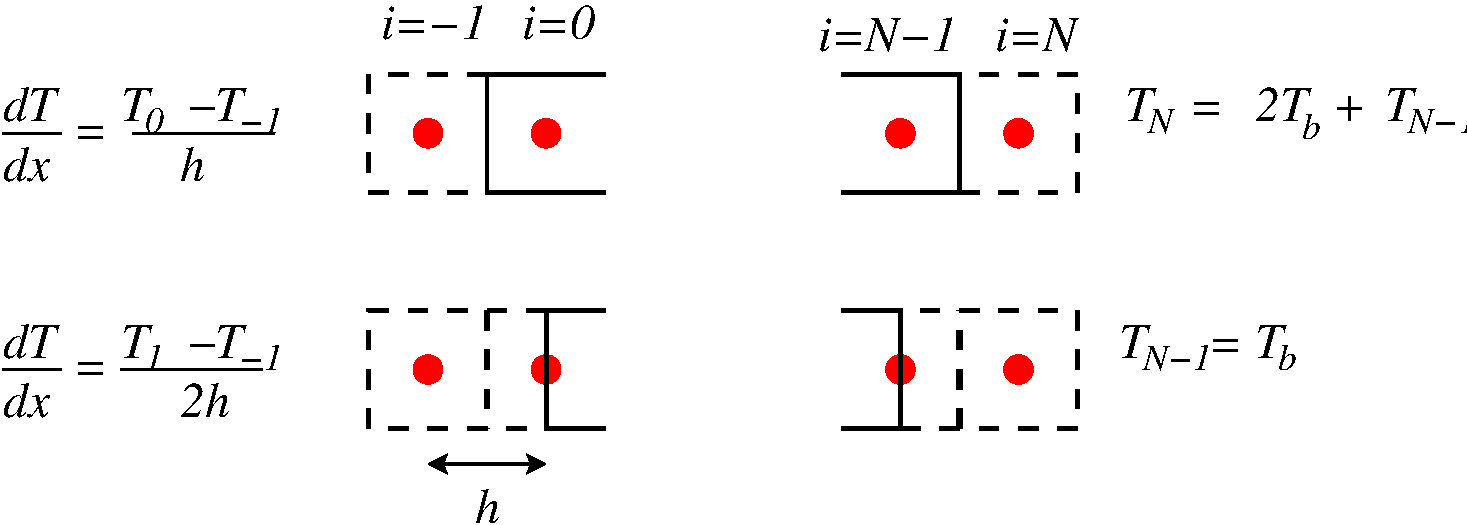
\includegraphics[width=1.0\linewidth]{fig-lin/bbc.pdf}}
  \caption{
  Flux boundary condition (Neumann), and value boundary condition (Dirichlet). For the upper right boundary condition we use Taylors formula to interpolate, see equation (\ref{eq:lin:dd}). \label{fig:lin:bbc}
  }
\end{figure}
%\clearpage % flush figures fig:lin:bbc



\begin{graybox2admon}[Example: Steady state heat equation as a linear problem]
Consider the case where we have 4 grid nodes and the outline of the simulation nodes are as in figure~\ref{fig:lin:grid} to the left, i.e.~nodes at the physical  boundaries. Assume a zero flux boundary condition to the left, and a constant temperature,$T_b$, to the right. Write the heat equation
\begin{equation}
k\frac{d^2T}{dx^2}+\kappa=0,
\label{eq:lin:exx1}
\end{equation}
as a matrix equation.

\paragraph{Solution:}
First, we use the discrete version of equation (\ref{eq:lin:exx1}) in equation (\ref{eq:lin:e3}) for $i=0, 1, 2, 3$
\begin{align}
T_{-1}+T_1-2T_0 &=-h^2\kappa/k,\nonumber \\ 
T_{0}+T_2-2T_1 &=-h^2\kappa/k\nonumber \\ 
T_{1}+T_3-2T_2 &=-h^2\kappa/k\nonumber \\ 
T_{2}+T_4-2T_3 &=-h^2\kappa/k.
\label{eq:lin:exx2}
\end{align}
Now, we have four equations, but six unknowns ($T_{-1}, T_0, T_1, T_2, T_3, T_4$). $T_{-1}$, and $T_4$ can be found from the boundary conditions. Using the formulas in figure~\ref{fig:lin:bbc} at the lower left and lower right, we get $dT/dx=0$, and $T_{-1}=T_1$, and $T_4=T_b$. Thus the first and last equation in equation (\ref{eq:lin:exx2}), can be written
\begin{align}
2T_1-2T_0 &=-h^2\kappa/k,\nonumber \\ 
T_{2}-2T_3 &=-h^2\kappa/k-T_b.
\label{eq:lin:2b}
\end{align}
Now, we can formulate equation (\ref{eq:lin:exx2}) as a matrix problem, with the unknowns on the left side and the unknown on the right hand side.
\begin{align}
\left(
\begin{array}{cccc}
-2&2&0&0\\ 
1&-2&1&0\\ 
0&1&-2&1\\ 
0&0&1&-2\\ 
\end{array}
\right)
\left(
\begin{array}{c}
T_0\\ 
T_1\\ 
T_2\\ 
T_3\\ 
\end{array}
\right)
=
\left(
\begin{array}{c}
-h^2\kappa/k\\ 
-h^2\kappa/k\\ 
-h^2\kappa/k\\ 
-h^2\kappa/k-T_b
\end{array}
\right).
\end{align}
\label{eq:lin:exx4}
\end{graybox2admon}



In principle, to discretize an equation is straight forward, but there are some 

First, we are going to consider a \emph{steady state} solution. Steady state means that the solution does no longer change as a function of time, i.e.~$dq/dt=0$ in equation (\ref{eq:lin:cont4}). We are also going to assume that the area is constant $A(x)=A$, thus the equation we want to solve is

\section{Solving linear equations}
There are a number of excellent books covering this topic, see e.g.~\cite{press2007,trefethen1997,stoer2013,strang2019}.
In most of the examples covered in this course we will encounter problems where we have a set of \emph{linearly independent} equations and one equation for each unknown. For these type of problems there are a number of methods that can be used, and they will find a solution in a finite number of steps. If a solution cannot be found it is usually because the equations are not linearly independent, and our formulation of the physical problem is wrong.

Assume that we would like to solve the following set of equations:
\begin{align}
2x_0+x_1+x_2+3x_3&=1, \label{eq:lin:la} \\ 
x_0+x_1+3x_2+x_3&=-3, \label{eq:lin:lb} \\ 
x_0+4x_1+x_2+x_3&=2, \label{eq:lin:lc} \\ 
x_0+x_1+2x_2+2x_3&=1. \label{eq:lin:ld} 
\end{align}
These equations can be written in matrix form as:
\begin{equation}
\mathbf{A\cdot x}=\mathbf{b},
\label{eq:lin:mat}
\end{equation}
where:
\begin{equation}
\mathbf{A}\equiv\begin{pmatrix}
2&1&1&3\\ 
1&1&3&1\\ 
1&4&1&1\\ 
1&1&2&2
\end{pmatrix}
\qquad
\mathbf{b}\equiv
\begin{pmatrix}
1\\-3\\2\\1
\end{pmatrix}
\qquad
\mathbf{x}\equiv
\begin{pmatrix}
x_0\\x_1\\x_2\\x_3
\end{pmatrix}.
\label{eq:lin:matA}
\end{equation}
You can easily verify that $x_0=-4, x_1=1, x_2=-1, x_3= 3$ is the
solution to the above equations by direct substitution. If we were to
replace one of the above equations with a linear combination of any of
the other equations, e.g.~replace equation (\ref{eq:lin:ld}) with
$3x_0+2x_1+4x_2+4x_3=-2$, there would be no unique solution (infinite
number of solutions). This can be checked by calculating the determinant of the matrix $\mathbf{A}$, if $\det \mathbf{A}=0 $,  
What is the difficulty in solving these equations? Clearly if none of the equations are linearly dependent, and we have $N$ independent linear equations, it should be straight forward to solve them? Two major numerical problems are i) even if the equations are not exact linear combinations of each other, they could be very close, and as the numerical algorithm progresses they could at some stage become linearly dependent due to roundoff errors. ii) roundoff errors may accumulate if the number of equations are large \cite{press2007}.

\subsection{Gauss-Jordan elimination}
\index{Gauss-Jordan elimination}
Let us continue the discussion by consider Gauss-Jordan elimination, which is a \emph{direct} method. A direct method uses a final set of operations to obtain a solution. According to \cite{press2007} Gauss-Jordan elimination is the method of choice if we want to find the inverse of $\mathbf{A}$. However, it is slow when it comes to calculate the solution of equation
(\ref{eq:lin:mat}). Even if speed and memory use is not an issue, it is also not advised to first find the inverse, $\mathbf{A}^{-1}$, of $\mathbf{A}$, then multiply it with $\mathbf{b}$ to obtain the solution, due to roundoff errors (Roundoff errors occur whenever we subtract to numbers that are very close to each other). To simplify our notation, we write equation (\ref{eq:lin:matA}) as:
\begin{equation}
\left(
\begin{array}{cccc|c}
2&1&1&3&1\\ 
1&1&3&1&-3\\ 
1&4&1&1&2\\ 
1&1&2&2&1
\end{array}
\right).
\end{equation}
The numbers to the left of the vertical dash is the matrix $\mathbf{A}$, and to the right is the vector $\mathbf{b}$. The Gauss-Jordan elimination procedure proceeds by doing the same operation on the right and left side of the dash, and the goal is to get only zeros on the lower triangular part of the matrix. This is achieved by multiplying rows with the same (nonzero) number, swapping rows, adding a multiple of a row to another:
\begin{align}
&\left(
\begin{array}{cccc|c}
2&1&1&3&1\\ 
1&1&3&1&-3\\ 
1&4&1&1&2\\ 
1&1&2&2&1
\end{array}
\right)\to
\left(
\begin{array}{cccc|c}
2&1&1&3&1\\ 
0&1/2&5/2&-1/2&-7/2\\ 
0&7/2&1/2&-1/2&3/2\\ 
0&1/2&3/2&1/2&1/2
\end{array}
\right)\to\label{eq:lin:gj1}\\ 
&\left(
\begin{array}{cccc|c}
2&1&1&3&1\\ 
0&1/2&5/2&-1/2&-7/2\\ 
0&0&-17&3&26\\ 
0&0&1&-1&4
\end{array}
\right)
\to
\left(
\begin{array}{cccc|c}
2&1&1&3&1\\ 
0&1/2&5/2&-1/2&-7/2\\ 
0&0&-17&3&26\\ 
0&0&0&14/17&42/17
\end{array}
\right)\no
\end{align}
The operations done are: ($1\to2$) multiply first row with $-1/2$ and add to second, third and the fourth row, ($2\to 3$) multiply second row with $-7$, and add to third row, multiply second row with $-1$ and add to fourth row, ($3\to4$) multiply third row with $-1/17$ and add to fourth row. These operations can easily be coded into Python:










\begin{lstlisting}[language=python,style=blue1]
A = np.array([[2, 1, 1, 3],[1, 1, 3, 1],
              [1, 4, 1, 1],[1, 1, 2, 2 ]],float)
b = np.array([1,-3,2,1],float)
N=4
# Gauss-Jordan Forward Elimination
for i in range(1,N):
    fact    = A[i:,i-1]/A[i-1,i-1]
    A[i:,] -= np.outer(fact,A[i-1,])
    b[i:]  -= b[i-1]*fact

\end{lstlisting}

The python code is a bit compact, below there is an implementation using for loops









\begin{lstlisting}[language=python,style=blue1bar]
# Gauss-Jordan Forward Elimination - for loops
for i in range(N):
    for j in range(i+1,N):
        fact    = A[j,i]/A[i,i]
        for k in range(i+1,N):
            A[j,k] = A[j,k]- fact*A[i,k]
        b[j]  = b[j]- b[j-1]*fact
	A[j,i]= 0. # alternatively k=i,...,N

\end{lstlisting}




\begin{graybox2admon}[Number of (long) operations]
The code above reveals that that there are quite a few multiplications or divisions being performed in the forward elimination. Multiplications and divisions are more time consuming than addition and subtraction, and are usually termed \emph{long} operations. Not all loops runs from zero to $N$, the innermost from $k=i+1\ldots N-1$, i.e.~a total of $N-i-2$, the second contains $N-i-2$ and one multiplication for the \texttt{b} vector. Hence we have number of long operations
\begin{equation}
\sum_{i=0}^{N-1}(N-i-2)^2+(N-i-2)=\frac{N}{3}(N^2-3N+2).
\label{}
\end{equation}
The important result is that when the system of equations becomes large $N^3\gg N^2$ and the algorithm scales as $N^3$.
\end{graybox2admon}



Notice that the final matrix has only zeros beyond the diagonal, such a matrix is called \emph{upper triangular}. We still have not found the final solution, but from an upper triangular (or lower triangular) matrix it is trivial to determine the solution. The last row immediately gives us $14/17z=42/17$ or $z=3$, now we have the solution for z and the next row gives: $-17y+3z=26$ or $y=(26-3\cdot3)/(-17)=-1$, and so on. In a more general form, we can write our solution of the matrix $\mathbf{A}$ after making it upper triangular as:
\begin{equation}
\begin{pmatrix}
a^\prime_{0,0}&a^\prime_{0,1}&a^\prime_{0,2}&a^\prime_{0,3}\\ 
0&a^\prime_{1,1}&a^\prime_{1,2}&a^\prime_{1,3}\\ 
0&0&a^\prime_{2,2}&a^\prime_{2,3}\\ 
0&0&0&a^\prime_{3,3}
\end{pmatrix}
\cdot
\begin{pmatrix}
x_0\\ 
x_1\\ 
x_2\\ 
x_3
\end{pmatrix}
=
\begin{pmatrix}
b^\prime_{0}\\ 
b^\prime_{1}\\ 
b^\prime_{2}\\ 
b^\prime_{3}
\end{pmatrix}
\label{eq:lin:back}
\end{equation}
The back substitution can then be written formally as:
\begin{equation}
x_i=\frac{1}{a^\prime_{ii}}\left[b_i^\prime-\sum_{j=i+1}^{N-1}a^\prime_{ij}x_j\right],\quad i=N-1,N-2,\ldots,0
\label{eq:lin:back2}
\end{equation}
The back substitution can now easily be implemented in Python as:






\begin{lstlisting}[language=python,style=blue1]
# Back substitution
sol = np.zeros(N,float)
sol[N-1]=b[N-1]/A[N-1,N-1]
for i in range(2,N+1):
    sol[N-i]=(b[N-i]-np.dot(A[(N-i),],sol))/A[N-i,N-i]

\end{lstlisting}

Notice that in the Python implementation, we have used vector operations instead of for loops. This makes the code more efficient, but it could also be implemented with for loops: 








\begin{lstlisting}[language=python,style=blue1]
# Back substitution - for loop
sol = np.zeros(N,float)
for i in range(N-1,-1,-1):
    sol[i]= b[i]
    for j in range(i+1,N):
        sol[i] -= A[i][j]*sol[j]
    sol[i] /= A[i][i]

\end{lstlisting}



\begin{graybox2admon}[Number of (long) operations]
As for the forward elimination, we can find how the backward substitution scales. Notice that here there are only two loops, hence we have number of long operations
\begin{equation}
\sum_{i=0}^{N-1}(N-i-1)=\frac{N}{2}(N-1).
\label{}
\end{equation}
Thus, the backward substitution scales as $N^2$.
\end{graybox2admon}



There are at least two things to notice with our implementation:
\begin{itemize}
\item Matrix and vector notation makes the code more compact and efficient. In order to understand the implementation it is advised to put $i=1, 2, 3, 4$, and then execute the statements in the Gauss-Jordan elimination and compare with equation (\ref{eq:lin:gj1}).

\item The implementation of the Gauss-Jordan elimination is not robust, in particular one could easily imagine cases where one of the leading coefficients turned out as zero, and the routine would fail when we divide by \texttt{A[i-1,i-1]}. By simply changing equation (\ref{eq:lin:lb}) to $2x_0+x_1+3x_2+x_3=-3$, when doing the first Gauss-Jordan elimination, both $x_0$ and $x_1$ would be canceled. In the next iteration we try to divide next equation by the leading coefficient of $x_1$, which is zero, and the whole procedure fails.
\end{itemize}

\noindent
\subsection{Pivoting}
\index{pivoting}
The solution to the last problem is solved by what is called \emph{pivoting}. The element that we divide on is called the \emph{pivot element}. It actually turns out that even if we do Gauss-Jordan elimination \emph{without} encountering a zero pivot element, the Gauss-Jordan procedure is numerically unstable in the presence of roundoff errors \cite{press2007}. There are two versions of pivoting, \emph{full pivoting} and \emph{partial pivoting}. In partial pivoting we only interchange rows, while in full pivoting we also interchange rows and columns. Partial pivoting is much easier to implement, and the algorithm is as follows:
\begin{enumerate}
\item Find the row in $\mathbf{A}$ with largest absolute value in front of $x_0$ and change with the first equation, switch corresponding elements in $\mathbf{b}$

\item Do one Gauss-Jordan elimination, find the row in $\mathbf{A}$ with the largest absolute value in front of $x_1$ and switch with the second (same for $\mathbf{b}$), and so on.
\end{enumerate}

\noindent
For a linear equation we can multiply with a number on each side and the equation would be unchanged, so if we where to multiply one of the equations with a large value, we are almost sure that this equation would be placed first by our algorithm. This seems a bit strange as our mathematical problem is the same. Sometimes the linear algebra routines tries to normalize the equations to find the pivot element that would have been the largest element if all equations were normalized according to some rule, this is called \emph{implicit pivoting}.  
\subsection{LU decomposition}
\index{LU decomposition}
As we have already seen, if the matrix $\mathbf{A}$ is reduced to a triangular form it is trivial to calculate the solution by using back substitution. Thus if it was possible to decompose the matrix $\mathbf{A}$ as follows:

\begin{equation}
\mathbf{A}=\mathbf{L}\cdot\mathbf{U}\label{eq:lin:lu}
\end{equation}

\begin{equation}
\begin{pmatrix}
a_{0,0}&a_{0,1}&a_{0,2}&a_{0,3}\\ 
a_{1,0}&a_{1,1}&a_{1,2}&a_{1,3}\\ 
a_{2,0}&a_{2,1}&a_{2,2}&a_{2,3}\\ 
a_{3,0}&a_{3,1}&a_{3,2}&a_{3,3}
\end{pmatrix}
=
\begin{pmatrix}
l_{0,0}&0&0&0\\ 
l_{1,0}&l_{1,1}&0&0\\ 
l_{2,0}&l_{2,1}&l_{2,2}&0\\ 
l_{3,0}&l_{3,1}&l_{3,2}&l_{3,3}
\end{pmatrix}
\cdot
\begin{pmatrix}
u_{0,0}&u_{0,1}&u_{0,2}&u_{0,3}\\ 
0&u_{1,1}&u_{1,2}&u_{1,3}\\ 
0&0&u_{2,2}&u_{2,3}\\ 
0&0&0&u_{3,3}
\end{pmatrix}.
\end{equation}
The solution procedure would then be to rewrite equation (\ref{eq:lin:mat}) as:
\begin{align}
\mathbf{A\cdot x}=\mathbf{L}\cdot\mathbf{U}\cdot\mathbf{x}=\mathbf{b},\label{eq:lin:matb}
\end{align}
If we define a new vector $\mathbf{y}$:
\begin{align}
\mathbf{y}\equiv\mathbf{U}\cdot\mathbf{x},
\end{align}
we can first solve for the $\mathbf{y}$ vector:
\begin{align}
\mathbf{L}\cdot\mathbf{y}=\mathbf{b},\label{eq:lin:for}
\end{align}
and then for $\mathbf{x}$:
\begin{align}
\mathbf{U}\cdot\mathbf{x}=\mathbf{y}.
\end{align}
Note that the solution to equation (\ref{eq:lin:for}) would be done by \emph{forward substitution}:
\begin{equation}
y_i=\frac{1}{l_{ii}}\left[b_i-\sum_{j=0}^{i-1}l_{ij}x_j\right],\quad i=1,2,\ldots N-1.
\label{eq:lin:back3}
\end{equation}
Why go to all this trouble? First of all it requires (slightly) less operations to calculate the LU decomposition and doing the forward and backward substitution than the Gauss-Jordan procedure discussed earlier. Secondly, and more importantly, is the fact that in many cases one would like to calculate the solution for different values of the $\mathbf{b}$ vector in equation (\ref{eq:lin:matb}). If we do the LU decomposition first we can calculate the solution quite fast using backward and forward substitution for any value of the $\mathbf{b}$ vector.

The NumPy function \href{{https://docs.scipy.org/doc/numpy/reference/generated/numpy.linalg.solve.html}}{\nolinkurl{solve}\footnote{\texttt{https://docs.scipy.org/doc/numpy/reference/generated/numpy.linalg.solve.html}}}, uses LU decomposition and partial pivoting, and we can find the solution to our previous problem simply by the following code:



\begin{lstlisting}[language=python,style=blue1]
from numpy.linalg import solve
x=solve(A,b)

\end{lstlisting}


\section{Iterative methods}
The methods described so far are what is called \emph{direct} methods. The direct methods for very large systems might suffer from round off errors. That means that even if the computer has found a solution, the solution is "polluted" by round off errors, or stated more clearly: your solution for $\mathbf{x}$, when entered into the original equation $\mathbf{A}\mathbf{x}\neq\mathbf{b}$. Below we will describe one trick, and two alternative methods to the direct methods.
\subsection{Iterative improvement}
The first method \cite{press2001} assumes that we already have solved the matrix equation (\ref{eq:lin:mat}), and obtained an \emph{estimate} $\mathbf{\hat{x}}$ of the true solution $\mathbf{x}$. Assume that $\mathbf{\hat{x}}=\mathbf{x}+\delta\mathbf{x}$, and that
\begin{equation}
\mathbf{A}\cdot\mathbf{\hat{x}}=\mathbf{A}\cdot(\mathbf{x}+\delta\mathbf{x})=\mathbf{b}+\delta\mathbf{b},
\label{eq:lin:itb}
\end{equation}
subtracting equation (\ref{eq:lin:mat}) we get
\begin{equation}
\mathbf{A}\cdot\delta\mathbf{x}=\delta\mathbf{b}.
\label{eq:lin:itb2}
\end{equation}
Solving equation (\ref{eq:lin:itb}) for $\delta\mathbf{b}$ an inserting in the equation above, we get
\begin{equation}
\mathbf{A}\cdot\delta\mathbf{x}=\mathbf{A}\cdot\mathbf{\hat{x}}-\mathbf{b}.
\label{eq:lin:itb3}
\end{equation}
The usefulness of this method assumes that we have already obtained the LU decomposition of $\mathbf{A}$, and if possible one should use a higher precision to calculate the right hand side, since there will be a lot of cancellations. Then the whole computational process it is simply to calculate the right hand side and backsubstitute. The improved solution is then obtained by subtracting $\delta\mathbf{x}$ from $\mathbf{\hat{x}}$.

\subsection{The Jacobi method}
\index{Jacobi method}
A completely different approach is the Jacobian method, which is simply to decompose the $\mathbf{A}$ matrix in the following way
\begin{equation}
\mathbf{A}=\mathbf{D}+\mathbf{R}
\label{eq:lin:DR}
\end{equation}

\begin{align}
&\begin{pmatrix}
a_{0,0}&a_{0,1}&a_{0,2}&a_{0,3}\\ 
a_{1,0}&a_{1,1}&a_{1,2}&a_{1,3}\\ 
a_{2,0}&a_{2,1}&a_{2,2}&a_{2,3}\\ 
a_{3,0}&a_{3,1}&a_{3,2}&a_{3,3}
\end{pmatrix}
\no\\ 
&=
\begin{pmatrix}
a_{0,0}&0&0&0\\ 
0&a_{1,1}&0&0\\ 
0&0&a_{2,2}&0\\ 
0&0&0&a_{3,3}
\end{pmatrix}
+
\begin{pmatrix}
0&a_{0,1}&a_{0,2}&a_{0,3}\\ 
a_{1,0}&0&a_{1,2}&a_{1,3}\\ 
a_{2,0}&a_{2,1}&0&a_{2,3}\\ 
a_{3,0}&a_{3,1}&a_{3,2}&0
\end{pmatrix}.
\label{eq:lin:DR2}
\end{align}
We can then write equation (\ref{eq:lin:mat}) as
\begin{equation}
\mathbf{D}\mathbf{x}=\mathbf{b}-\mathbf{R}\cdot\mathbf{x}.
\label{eq:lin:jc}
\end{equation}
How does this help us? First of all, the matrix $\mathbf{D}$ is easy to invert as it is diagonal, the inverse can be found by simply replace $a_{ii}\to 1/a_{ii}$. But $\mathbf{x}$ is still present on the right hand side? This is where the \emph{iterations} comes into play, we simply guess at an initial solution $\mathbf{x}^k$, and then we use equation (\ref{eq:lin:jc}) to calculate the next solution $\mathbf{x}^{k+1}$, and so on
\begin{equation}
\mathbf{x}^{k+1}=\mathbf{D}^{-1}(\mathbf{b}-\mathbf{R}\cdot\mathbf{x}^{k}).
\label{eq:lin:jc2}
\end{equation}
Lets write it out on component form for a $4\times4$ matrix to see what is going on
\begin{align}
x_0^{k+1} &=\frac{1}{a_{00}}(b_0-a_{01}x_1^k-a_{02}x_2^k-a_{03}x_3^k),
\label{eq:lin:jc3a}\\ 
x_1^{k+1} &=\frac{1}{a_{11}}(b_1-a_{10}x_0^k-a_{12}x_2^k-a_{13}x_3^k),
\label{eq:lin:jc3b}\\ 
x_2^{k+1} &=\frac{1}{a_{22}}(b_2-a_{20}x_0^k-a_{21}x_1^k-a_{23}x_3^k),
\label{eq:lin:jc3c}\\ 
x_3^{k+1} &=\frac{1}{a_{33}}(b_3-a_{30}x_0^k-a_{31}x_1^k-a_{32}x_2^k).
\label{eq:lin:jc3d}
\end{align}
Below is a Python implementation






















\begin{lstlisting}[language=python,style=blue1]
def solve_jacobi(A,b,x=-1,w=1,max_iter=1000,EPS=1e-6):
    """
    Solves the linear system Ax=b using the Jacobian method, stops if
    solution is not found after max_iter or if solution changes less 
    than EPS
    """
    if(x==-1): #default guess 
        x=np.zeros(len(b))
    D=np.diag(A)
    R=A-np.diag(D)
    eps=1
    x_old=x
    iter=0
    w=0.1
    while(eps>EPS and iter<max_iter):
        iter+=1
        x=w*(b-np.dot(R,x_old))/D + (1-w)*x_old
        eps=np.sum(np.abs(x-x_old))
        x_old=x
    print('found solution after ' + str(iter) +' iterations')
    return x

\end{lstlisting}

A sufficient criteria for the Jacobian method to converge is if the matrix $A$ is diagonally dominant. In the implementation above we have included a weight, which sometimes can help in the convergence even if the matrix is not diagonally dominant. 

The iterative method can be appealing if we do not need a high accuracy, we can choose to stop whenever $|\mathbf{x}^{k+1}-\mathbf{x}^k|$ is small enough. For the direct method we have to follow through all the way.


\begin{graybox2admon}[Convergence]
The Jacobi method converges if the matrix $\mathbf{A}$ is strictly diagonally dominant. Strictly diagonally dominant means that the absolute value of each entry on the diagonal is greater than the sum of the absolute values of the other entries in the same row, i.e if $|a_{00}|>|a_{01}+a_{02}+\cdots|$. In general it can be shown that a iterative scheme $\mathbf{x}^{k+1}=\mathbf{P}\cdot \mathbf{x}^k+\mathbf{q}$ is convergent \emph{if and only if} every eigenvalue, $\lambda$, of $\mathbf{P}$ satisfies $|\lambda|<1$, i.e.~the \emph{spectral radius} $\rho(\mathbf{P})<1$.
\end{graybox2admon}




\subsection{The Gauss-Seidel method}
\index{Gauss-Seidel method}
It is tempting in equation (\ref{eq:lin:jc3a}) to use our estimate of $x_0^{k+1}$ in the next equation, equation (\ref{eq:lin:jc3b}), instead of $x_0^k$. After all our estimate $x_0^{k+1}$ is an \emph{improved} estimate. This is actually the Gauss-Seidel method. This method also has the advantage that if there are memory issues, one can overwrite the old value of $x_i^k$. Usually the Gauss-Seidel method converges faster, but not always. A plus for the Jacobi method is that is can be  parallelised, as the calculations is only dependent on the old values and do not require information about the new values as for the Gauss Seidel method. Below is a Python implementation of the Gauss-Seidel method   























\begin{lstlisting}[language=python,style=blue1]
def solve_GS(A,b,x=-1,max_iter=1000,EPS=1e-6):
    """
    Solves the linear system Ax=b using the Gauss-Seidel method, stops if
    solution is not found after max_iter or if solution changes less 
    than EPS
    """
    if(x==-1):
        x=np.zeros(len(b))
    D=np.diag(A)
    R=A-np.diag(D)
    eps=1
    iter=0
    while(eps>EPS and iter<max_iter):
        iter+=1
        eps=0.
        for i in range(len(x)):
            tmp=x[i]
            x[i]=(b[i]- np.dot(R[i,:],x))/D[i]
            eps+=np.abs(tmp-x[i])
    print('found solution after ' + str(iter) +' iterations')
    return x

\end{lstlisting}


\section{Example: Linear regression}
\index{linear regression}
In the previous section, we considered a system of $N$ equations and $N$ unknown ($x_0, x_1,\ldots, x_N$). In general we might have more equations than unknowns or more unknowns than equations. An example of the former is linear regression, we might have many data points and we would like to fit a line through the points. How do you fit a single lines to more than two points that does not line on the same line? One way to do it is to minimize the distance from the line to the points, as illustrated in figure~\ref{fig:lin:reg}.

\begin{figure}[!ht]  % fig:lin:reg
  \centerline{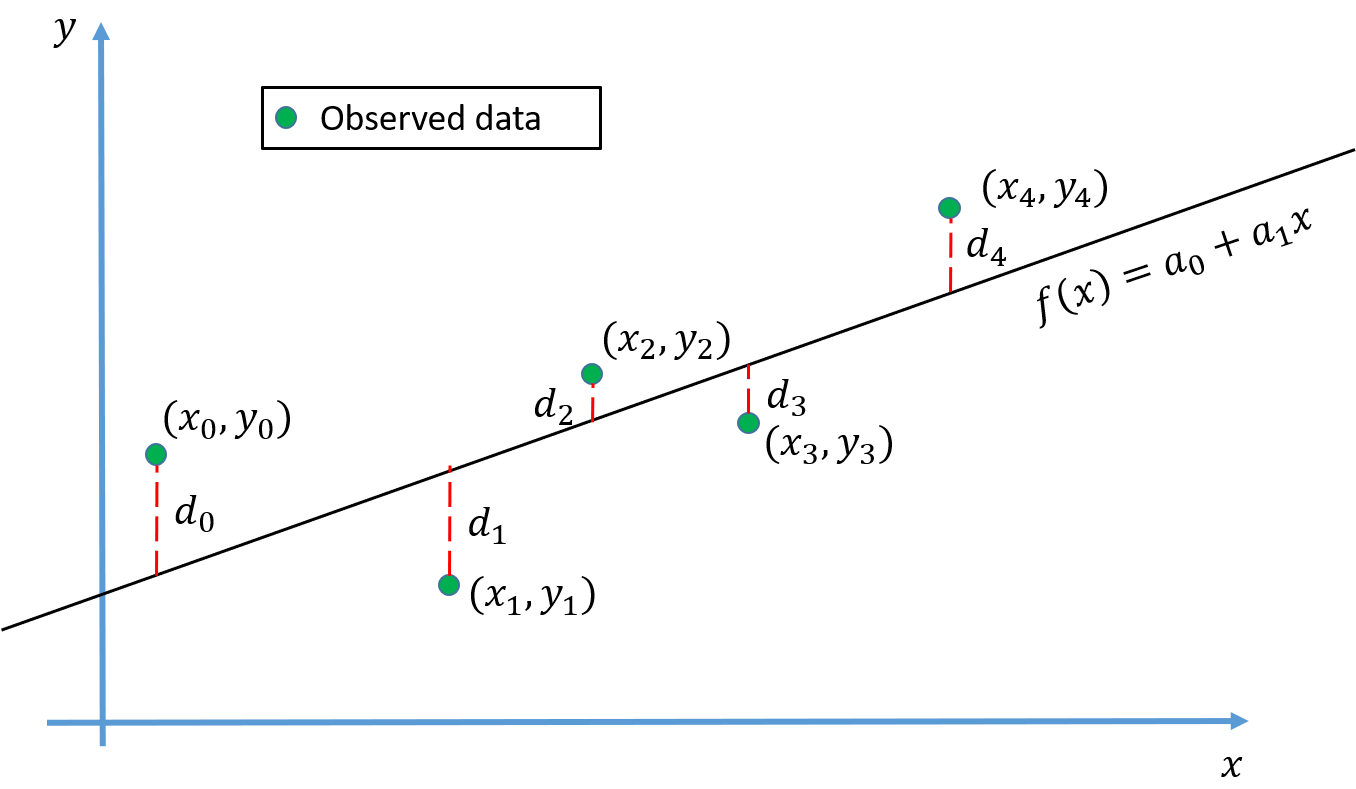
\includegraphics[width=0.9\linewidth]{fig-lin/reg.png}}
  \caption{
  Linear regression by minimizing the total distance to all the points. \label{fig:lin:reg}
  }
\end{figure}
%\clearpage % flush figures fig:lin:reg

Mathematically we can express the distance between a data point $(x_i,y_i)$ and the line $f(x)$ as $y_i-f(x_i)$. Note that this difference can be negative or positive depending if the data point lies below or above the line. We can then take the absolute value of all the distances, and try to minimize them. When we minimize something we take the derivative of the expression and put it equal to zero.  As you might remember from Calculus it is extremely hard to work with the derivative of the absolute value, because it is discontinuous. A much better approach is to square each distance and sum them:
\begin{equation}
S=\sum_{i=0}^{N-1}(y_i-f(x_i))^2=\sum_{i=0}^{N-1}(y_i-a_0-a_1x_i)^2.
\label{eq:lin:lsq}
\end{equation}
(For the example in figure~\ref{fig:lin:reg}, $N=5$.) This is the idea behind \emph{least square}, and linear regression. One thing you should be aware of is that points lying far from the line will contribute more to equation (\ref{eq:lin:lsq}). The underlying assumption is that each data point provides equally precise information about the process, this is often not the case. When analyzing experimental data, there may be points deviating from the expected behaviour, it is then important to investigate if these points are more affected by measurements errors than the others. If that is the case one should give them less weight in the least square estimate, by extending the formula above:
\begin{equation}
S=\sum_{i=0}^{N-1}\omega_i(y_i-f(x_i))^2=\sum_{i=0}^3\omega_i(y_i-a_0-a_1x_i)^2,
\label{eq:lin:lsqm}
\end{equation}
$\omega_i$ is a weight factor.

\subsection{Solving least square, using algebraic equations}
Let us continue with equation (\ref{eq:lin:lsq}), the algebraic solution is to simply find the value of $a_0$ and $a_1$ that minimizes $S$:
\begin{align}
\frac{\partial S}{\partial a_0} &=-2\sum_{i=0}^{N-1}(y_i-a_0-a_1x_i)=0,
\label{eq:lin:ls1} \\ 
\frac{\partial S}{\partial a_1} &=-2\sum_{i=0}^{N-1}(y_i-a_0-a_1x_i)x_i=0.
\label{eq:lin:ls2}
\end{align}
Defining the mean value as $\overline{x}=\sum_ix_i/N$ and $\overline{y}=\sum_iy_i/N$, we can write equation (\ref{eq:lin:ls1}) and (\ref{eq:lin:ls2})  as:
\begin{align}
\sum_{i=0}^{N-1}(y_i-a_0-a_1x_i)&=N\overline{y}-a_0N-a_1N\overline{x}=0,
\label{eq:lin:ls1a} \\ 
\sum_{i=0}^{N-1}(y_i-a_0-a_1x_i)x_i&=\sum_iy_ix_i-a_0N\overline{x}-a_1\sum_ix_ix_i=0.
\label{eq:lin:ls2b}
\end{align}
Solving equation (\ref{eq:lin:ls1a}) with respect to $a_0$, and inserting the expression into equation (\ref{eq:lin:ls2b}), we find:
\begin{align}
a_0&=\overline{y}-a_1\overline{x},\label{eq:lin:ls1c} \\ 
a_1&=\frac{\sum_iy_ix_i-N\overline{x}\overline{y}}{\sum_ix_i^2-N\overline{x}^2}
=\frac{\sum_i(x_i-\overline{x})(y_i-\overline{y})}{\sum_i(x_i-\overline{x})^2}.
\label{eq:lin:ls2d}
\end{align}
We leave it as an exercise to show the last expression for $a_1$.  
Clearly the equation (\ref{eq:lin:ls2d}) above will in most cases have
a solution. But in addition to a solution, it would be good to have an
idea of the goodness of the fit. Intuitively it make sense to add all
the distances (residuals) $d_i$ in figure~\ref{fig:lin:reg}. This is
basically what is done when calculating $R^2$ (R-squared). However, we
would also like to compare the $R^2$ between different
datasets. Therefor we need to normalize the sum of residuals, and
therefore the following form of the $R^2$ is used:
\begin{equation}
R^2=1-\frac{\sum_{i=0}^{N-1}(y_i-f(x_i))^2}{\sum_{i=0}^{N-1}(y_i-\overline{y})^2}.
\label{eq:lin:r2}
\end{equation}
In python we can implement equation (\ref{eq:lin:ls1c}), (\ref{eq:lin:ls2d}) and (\ref{eq:lin:r2}) as:



























\begin{lstlisting}[language=python,style=blue1]
def OLS(x, y): 
    # returns regression coefficients
    # in ordinary least square
    # x: observations
    # y: response
    # R^2: R-squared
    n = np.size(x) # number of data points 
  
    # mean of x and y vector 
    m_x, m_y = np.mean(x), np.mean(y) 
  
    # calculating cross-deviation and deviation about x 
    SS_xy = np.sum(y*x) - n*m_y*m_x 
    SS_xx = np.sum(x*x) - n*m_x*m_x 
  
    # calculating regression coefficients 
    b_1 = SS_xy / SS_xx 
    b_0 = m_y - b_1*m_x

    #R^2
    y_pred = b_0 + b_1*x
    S_yy   = np.sum(y*y) - n*m_y*m_y
    y_res  = y-y_pred  
    S_res  = np.sum(y_res*y_res)
  
    return(b_0, b_1,1-S_res/S_yy)

\end{lstlisting}


\subsection{Least square as a linear algebra problem}
It turns out that the least square problem can be formulated as a
matrix problem. (Two great explanations see \href{{https://medium.com/@andrew.chamberlain/the-linear-algebra-view-of-least-squares-regression-f67044b7f39b}}{linear regression by
matrices}\footnote{\texttt{https://medium.com/@andrew.chamberlain/the-linear-algebra-view-of-least-squares-regression-f67044b7f39b}},
and
\href{{https://medium.com/@andrew.chamberlain/a-more-elegant-view-of-r-squared-a0a14c177dc3}}{$R^2$-squared}\footnote{\texttt{https://medium.com/@andrew.chamberlain/a-more-elegant-view-of-r-squared-a0a14c177dc3}}.)
If we define a matrix $\mathbf{X}$ containing the observations $x_i$
as:
\begin{align}
\mathbf{X} &=
\begin{pmatrix}
1&x_0\\ 
1&x_1\\ 
\vdots&\vdots\\ 
1&x_{N-1}
\end{pmatrix}.
\label{eq:lin:mreg1}
\end{align}
We introduce a vector containing all the response $\mathbf{y}$, and the
regression coefficients $\mathbf{a}=(a_0,a_1)$. Then we can write
equation (\ref{eq:lin:lsqm}) as a matrix equation:
\begin{equation}
S=(\mathbf{y}-\mathbf{X\cdot a})^T(\mathbf{y}-\mathbf{X\cdot a}).
\label{eq:lin:mregS}
\end{equation}
\emph{Note that this equation can easily be extended to more than one
observation variable $x_i$}. By simply differentiating equation
(\ref{eq:lin:mregS}) with respect to $\mathbf{a}$, we can show that
the derivative has a minimum when (see proof below):
\begin{equation}
\mathbf{X}^T\mathbf{X a}=\mathbf{X}^T\mathbf{y}
\label{eq:lin:mregS2}
\end{equation}
Below is a python implementation of equation (\ref{eq:lin:mregS2}).












\begin{lstlisting}[language=python,style=blue1]
def OLSM(x, y): 
    # returns regression coefficients
    # in ordinary least square using solve function
    # x: observations
    # y: response

    XT = np.array([np.ones(len(x)),x],float)
    X  = np.transpose(XT)
    B = np.dot(XT,X)
    C = np.dot(XT,y)
    return solve(B,C)

\end{lstlisting}


\subsection{Working with matrices on component form}
Whenever you want to do some manipulation with matrices, it is very useful to simply write them on component form. If we multiply two matrices $\mathbf{A}$ and $\mathbf{B}$ to form a new matrix $\mathbf{C}$, the components of the new matrix is simply $\mathbf{C}_{ij}=\sum_k\mathbf{A}_{ik}\mathbf{B}_{kj}$. The strength of doing this is that the elements of a matrix, e.g.~$\mathbf{A}_{ik}$ are \emph{numbers}, and we can move them around. Proving that e.g.~$(\mathbf{A}\mathbf{B})^T=\mathbf{B}^T\mathbf{A}^T$ is straight forward using the component form. The transpose of a matrix is simply to exchange columns and rows, hence $\mathbf{C}_{ij}^T=\mathbf{C}_{ji}$
\begin{equation}
\mathbf{C}_{ij}^T=\mathbf{C}_{ji}=\sum_k\mathbf{A}_{jk}\mathbf{B}_{ki}=\sum_k\mathbf{B}^T_{ik}\mathbf{A}^T_{kj}
=(\mathbf{B}^T\mathbf{A}^T)_{ij},
\label{eq:lin:trans}
\end{equation}
thus $\mathbf{C}^T=\mathbf{B}^T\mathbf{A}^T$. To derive equation (\ref{eq:lin:mregS2}), we need to take the derivative of equation (\ref{eq:lin:mregS2}) with respect to $\mathbf{a}$.
What we mean by this is that we want to evaluate $\partial S/\partial a_k$ for all the components of $\mathbf{a}$.
A useful rule is $\partial a_i/\partial a_k=\delta_{ik}$, where $\delta_{ik}$ is the Kronecker delta, it takes the value of one if $i=k$ and zero otherwise. We can write $S=\mathbf{y}^T\mathbf{y}-\mathbf{y}\mathbf{X\cdot a}
-(\mathbf{X\cdot a})^T\mathbf{y}-(\mathbf{X\cdot a})^T\mathbf{X\cdot a}$. All terms that do not contain $\mathbf{a}$ are zero, thus we only need to evaluate the following terms
\begin{align}
\frac{\partial}{a_k}(\mathbf{X\cdot a})^T\mathbf{y} &=\frac{\partial}{a_k}(\mathbf{a}^T\cdot \mathbf{X}^T\mathbf{y})=\frac{\partial}{a_k}\sum_{ij}\mathbf{a}^T_i\mathbf{X}^T_{ij}\mathbf{y}_j
=\sum_{ij}\delta_{ik}\mathbf{X}^T_{ij}\mathbf{y}_j\no\\ 
&=\sum_{j}\mathbf{X}^T_{kj}\mathbf{y}_j=\mathbf{X}^T\mathbf{y} \\ 
\frac{\partial}{a_k}\mathbf{y}^T\mathbf{X\cdot a}&=\frac{\partial}{a_k}\sum_{ij}\mathbf{y}^T_i\mathbf{X}_{ij}\mathbf{a}_j
=\sum_{ij}\mathbf{y}^T_i\mathbf{X}_{ij}\delta_{jk}=\sum_{j}\mathbf{y}^T_{i}\mathbf{X}_{ik}\no\\ 
&=\sum_{j}\mathbf{y}^T_{i}\mathbf{X}^T_{ki}=\mathbf{X}^T\mathbf{y} \\ 
\frac{\partial}{a_k} (\mathbf{X\cdot a})^T\mathbf{X\cdot a}&=
\frac{\partial}{a_k}\sum_{ijl} \mathbf{a}^T_i\mathbf{X}^T_{ij}\mathbf{X}_{jl}\mathbf{a}_l=
\sum_{ijl}(\delta_{ik}\mathbf{X}^T_{ij}\mathbf{X}_{jl}\mathbf{a}_l+\mathbf{a}^T_i\mathbf{X}^T_{ij}\mathbf{X}_{jl}\delta_{lk})\no\\&=\sum_{jl}\mathbf{X}^T_{kj}\mathbf{X}_{jl}
\mathbf{a}_l+\sum_{ij}\mathbf{a}^T_i\mathbf{X}^T_{ij}\mathbf{X}_{jk}\no\\ 
&=\mathbf{X}^T\mathbf{X}\mathbf{a}+\sum_{ij}\mathbf{X}^T_{kj}\mathbf{X}_{ji}\mathbf{a}_i
= 2\mathbf{X}^T\mathbf{X}\mathbf{a}.
\label{}
\end{align}
It then follows that $\partial S/\partial \mathbf{a} = 0$ when
\begin{equation}
\mathbf{X}^T\mathbf{X a}=\mathbf{X}^T\mathbf{y}.
\label{eq:lin:matpr}
\end{equation}

\section{Sparse matrices and Thomas algorithm}
\index{sparse matrix}
\index{Thomas algorithm}
In many practical examples, such as solving partial differential
equations the matrices could be quite large and also contain a lot of
zeros. A very important class of such matrices are \emph{banded matrices}
this is a type of \emph{sparse matrices} containing a lot of zero elements,
and the non-zero elements are confined to diagonal bands. In the
following we will focus on one important type of sparse matrix the
tridiagonal. In the next section we will show how it enters naturally
in solving the heat equation. It turns out that solving banded
matrices is quite simple, and can be coded quite efficiently. As with
the Gauss-Jordan example, lets consider a concrete example:
\begin{align}
&\left(
\begin{array}{ccccc|c}
b_0&c_0&0&0&0&r_0\\ 
a_1&b_1&c_1&0&0&r_1\\ 
0&a_2&b_2&c_2&0&r_2\\ 
0& 0&a_3&b_3&c_3&r_3\\ 
0& 0& 0&a_4&b_4&r_4
\end{array}
\right)
\end{align}
The right hand side is represented with $r_i$. The first Gauss-Jordan
step is simply to divide by $b_0$, then we multiply with $-a_1$ and
add to second row:
\begin{align}
\to \left(
\begin{array}{ccccc|c}
1&c_0^\prime&0&0&0&r_0^\prime\\ 
0&b_1-a_1c_0^\prime&c_1&0&0&r_1-a_0r_0^\prime\\ 
0&a_2&b_2&c_2&0&r_2\\ 
0& 0&a_3&b_3&c_3&r_3\\ 
0& 0& 0&a_4&b_4&r_4
\end{array}
\right),
\end{align}
Note that we have introduced some new symbols to simplify the
notation: $c_0^\prime=c_0/b_0$ and $r_0^\prime=r_0/b_0$. Then we
divide by $b_1-a_1c_0^\prime$:
\begin{align}
&\left(
\begin{array}{ccccc|c}
1&c_0^\prime&0&0&0&r_0^\prime\\ 
0&1&c_1^\prime&0&0&r_1^\prime\\ 
0&a_2&b_2&c_2&0&r_2\\ 
0& 0&a_3&b_3&c_3&r_3\\ 
0& 0& 0&a_4&b_4&r_4
\end{array}
\right),
\end{align}
where $c_1^\prime=c_1/(b_1-a_1c_0^\prime)$ and
$r_1^\prime=(r_1-a_0r_0^\prime)/(b_1-a_1c_0^\prime)$. If you continue
in this manner, you can easily convince yourself that to transform a
tridiagonal matrix to the following form:
\begin{align}
\to \left(
\begin{array}{ccccc|c}
1&c_0^\prime&0&0&0&r_0^\prime\\ 
0&1&c_1^\prime&0&0&r_1^\prime\\ 
0&0&1&c_2^\prime&0&r_2^\prime\\ 
0& 0&0&1&c_3^\prime&r_3^\prime\\ 
0& 0& 0&0&1&r_4^\prime
\end{array}
\right),
\end{align}
where:
\begin{align}
c_0^\prime =\frac{c_0}{b_0} \qquad &r_0^\prime=\frac{r_0}{b_0}
\label{eq:lin:th0} \\ 
c_i^\prime
=\frac{c_i}{b_i-a_ic_{i-1}^\prime}\qquad
&r_i^\prime=\frac{r_i-a_ir_{i-1}^\prime}{b_i-a_ic_{i-1}^\prime}
\quad\text{, for }i=1,2,\ldots,N-1\label{eq:lin:thi} 
\end{align}
Note that we where able to reduce the tridiagonal matrix to an \emph{upper
triangular} matrix in only \emph{one} Gauss-Jordan step. This equation can
readily be solved using back-substitution, which can also be
simplified as there are a lot of zeros in the upper part. Let us
denote the unknowns $x_i$ as we did for the Gauss-Jordan case, now we
can find the solution as follows:
\begin{align}
x_{N-1} & = r_{N-1}^\prime \label{eq:lin:this0} \\ 
x_i     & = r_i^\prime-x_{i+1}c_i^\prime\quad\text{, for } i=N-2,N-3,\ldots,0
\label{eq:lin:thisi}
\end{align}
Equation (\ref{eq:lin:th0}), (\ref{eq:lin:thi}), (\ref{eq:lin:this0})
and (\ref{eq:lin:thisi}) is known as the Thomas algorithm after
Llewellyn Thomas. 


\begin{graybox2admon}[Notice]
Clearly tridiagonal matrices can be solved much more efficiently with
the Thomas algorithm than
using a standard library, such as LU-decomposition. This is
because the solution method takes advantages of the \emph{symmetry} of the
problem. We will not show it here, but it can be shown that the Thomas
algorithm is stable whenever $|b_i|\ge |a_i|+|c_i|$. If the algorithm
fails, an advice is first to use the standard \texttt{solve} function in
python. If this gives a solution, then \emph{pivoting} combined with the
Thomas algorithm might do the trick.
\end{graybox2admon}



\section{Example: Solving the heat equation using linear algebra}

% --- begin exercise ---
\begin{doconceexercise}
\refstepcounter{doconceexercisecounter}

\exercisesection{Exercise \thedoconceexercisecounter: Conservation Equation or the Continuity Equation}
                             

\begin{figure}[!ht]  % fig:nlin:heat
  \centerline{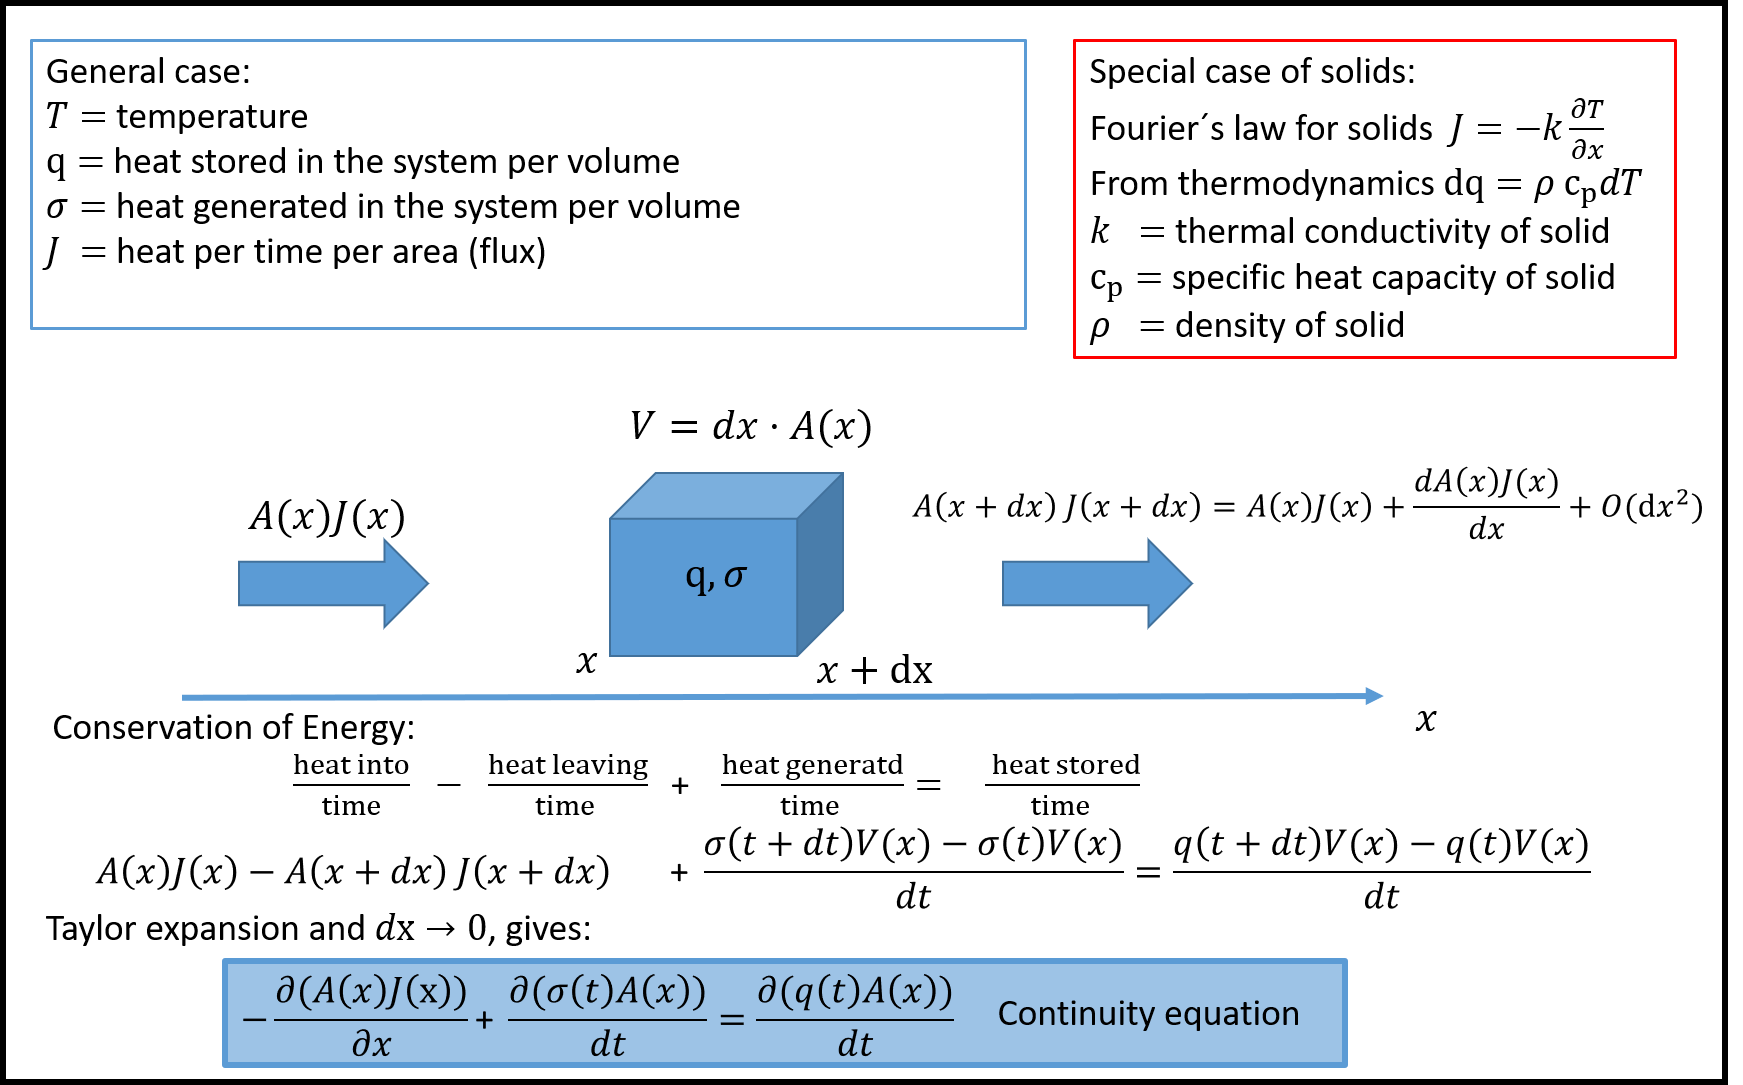
\includegraphics[width=0.9\linewidth]{fig-lin/heat.png}}
  \caption{
  Conservation of energy and the continuity equation. \label{fig:nlin:heat}
  }
\end{figure}
%\clearpage % flush figures fig:nlin:heat

In figure~\ref{fig:nlin:heat}, the continuity equation is derived for
heat flow.
\paragraph{Heat equation for solids.}
As derived in the beginning of this chapter the heat equation for a solid is
\begin{equation}
\frac{d^2T}{dx^2}+\frac{\dot{\sigma}}{k}=\frac{\rho c_p}{k}\frac{dT}{dt},
\label{eq:nlin:heateq}
\end{equation}
where $\dot{\sigma}$ is the rate of heat generation in the solid. This
equation can be used as a starting point for many interesting
models. In this exercise we will investigate the \emph{steady state}
solution, \emph{steady state} is just a fancy way of expressing that we
want the solution that \emph{does not change with time}. This is achieved
by ignoring the derivative with respect to time in equation
(\ref{eq:nlin:heateq}). We want to study a system with size $L$, and is
it good practice to introduce a dimensionless variable: $y=x/L$. 

\paragraph{Part 1.}

Show that equation (\ref{eq:nlin:heateq}) now takes the following form:
\begin{equation}
\frac{d^2T }{dy^2}+\frac{\dot{\sigma}L^2}{k}=0
\label{eq:nlin:heat2}
\end{equation}

\end{doconceexercise}
% --- end exercise ---

% --- begin exercise ---
\begin{doconceexercise}
\refstepcounter{doconceexercisecounter}

\exercisesection{Exercise \thedoconceexercisecounter: Curing of Concrete and Matrix Formulation}
                             

Curing of concrete is one particular example that we can investigate
with equation (\ref{eq:nlin:heat2}). When concrete is curing, there are
a lot of chemical reactions happening, these reactions generate
heat. This is a known issue, and if the temperature rises too much 
compared to the surroundings, the concrete may fracture.  In the
following we will, for simplicity, assume that the rate of heat
generated during curing is constant, $\dot{\sigma}=$100 W/m$^3$. The
left end (at $x=0$) is insulated, meaning that there is no flow of
heat over that boundary, hence $dT/dx=0$ at $x=0$. On the right hand
side the temperature is kept constant, $x(L)=y(1)=T_1$, assumed to be
equal to the ambient temperature of $T_1=25^\circ$C.  The concrete
thermal conductivity is assumed to be $k=1.65$ W/m$^\circ$C.

\paragraph{Part 1.}

Show that the solution to equation (\ref{eq:nlin:heat2}) in this case is:
\begin{equation}
T(y)=\frac{\dot{\sigma}L^2}{2k}(1-y^2)+T_1.
\label{eq:nlin:heatsol}
\end{equation}

\paragraph{Part 2.}
In order to solve equation (\ref{eq:nlin:heat2}) numerically, we need to discretize
it. Show that equation (\ref{eq:nlin:heat2}) now takes the following form:

\begin{equation}
T_{i+1}+T_{i-1}-2T_i=-h^2\beta,
\label{eq:nlin:heat3}
\end{equation}
where $\beta=\dot{\sigma}L^2/k$.

\begin{figure}[!ht]  % fig:nlin:hgrid
  \centerline{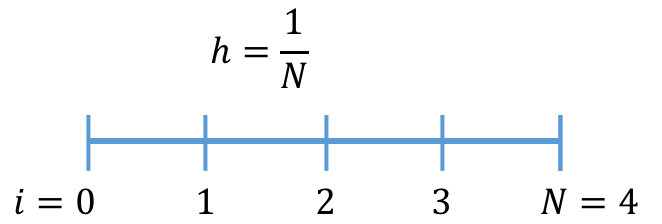
\includegraphics[width=0.5\linewidth]{fig-lin/heat_grid.png}}
  \caption{
  Finite difference grid for $N=4$. \label{fig:nlin:hgrid}
  }
\end{figure}
%\clearpage % flush figures fig:nlin:hgrid

In figure~\ref{fig:nlin:hgrid}, the finite difference grid is shown for
$N=4$.

\paragraph{Part 3.}

Show that equation (\ref{eq:nlin:heat3}) including the boundary conditions for $N=4$ can be written as the following matrix equation
\begin{align}
\left(
\begin{array}{cccc}
-\gamma&\gamma&0&0\\ 
1&-2&1&0\\ 
0&1&-2&1\\ 
0&0&1&-2\\ 
\end{array}
\right)
\left(
\begin{array}{c}
T_0\\ 
T_1\\ 
T_2\\ 
T_3\\ 
\end{array}
\right)
=
\left(
\begin{array}{c}
-h^2\beta\\ 
-h^2\beta\\ 
-h^2\beta\\ 
-h^2\beta-25
\end{array}
\right).
\end{align}
\label{eq:lin:heats}
where $\gamma=2$ for the central difference scheme and 1 for the forward difference scheme.

\paragraph{Part 4.}
\begin{itemize}
\item Solve the set of equations in equation (\ref{eq:lin:heats}) using \href{{https://numpy.org/doc/stable/reference/generated/numpy.linalg.solve.html}}{\nolinkurl{numpy.linalg.solve}\footnote{\texttt{https://numpy.org/doc/stable/reference/generated/numpy.linalg.solve.html}}}.

\item Write the code so that you can easily switch between the central difference scheme and forward difference

\item Evaluate the numerical error as you change $h$, how does it scale? Is it what you expect?
\end{itemize}

\noindent






\begin{lstlisting}[language=python,style=blue1]
import numpy as np
import scipy as sc
import scipy.sparse.linalg
from numpy.linalg import solve
import matplotlib.pyplot as plt

\end{lstlisting}














































\begin{lstlisting}[language=python,style=blue1]

central_difference=False
# set simulation parameters
h=0.25
L=1.0
n = int(round(L/h))
Tb=25 #rhs
sigma=100
k=1.65 
beta = sigma*L**2/k

y = np.arange(n+1)*h

def analytical(x):
    return beta*(1-x*x)/2+Tb
def tri_diag(a, b, c, k1=-1, k2=0, k3=1):
    """ a,b,c diagonal terms
        default k-values for 4x4 matrix:
        | b0 c0 0  0 |
        | a0 b1 c1 0 |
        | 0  a1 b2 c2|
        | 0  0  a2 b3|
    """
    return np.diag(a, k1) + np.diag(b, k2) + np.diag(c, k3)
# defina a, b and c vector
a=np.ones(n-1)
b=..
c=..

if central_difference:
    c[0]= ...
else:
    b[0]=...

A=tri_diag(a,b,c)
print(A) # view matrix - compare with N=4 to make sure no bugs
# define rhs vector
d=...
#rhs boundary condition
d[-1]=...

Tn=np.linalg.solve(A,d)
print(Tn)

\end{lstlisting}

The correct solution for $L=1$ m, and $h=1/4$, is: $[T_0,T_1.T_2,T_3]$=[55.3030303 , 53.40909091, 47.72727273, 38.25757576] (central difference) and $[T_0,T_1.T_2,T_3]$=[62.87878788, 59.09090909, 51.51515152, 40.15151515] (forward difference)

\end{doconceexercise}
% --- end exercise ---

% --- begin exercise ---
\begin{doconceexercise}
\refstepcounter{doconceexercisecounter}

\exercisesection{Exercise \thedoconceexercisecounter: Solve the full heat equation}
                             

\paragraph{Part 1.}
Replace the time derivative in equation (\ref{eq:nlin:heateq}) with
\begin{equation}
\frac{dT}{dt}\simeq\frac{T(t+\Delta t)-T(t)}{\Delta t}=\frac{T^{n+1}-T^n}{\Delta t}, 
\label{eq:lin:dt}
\end{equation}
and show that by using an \emph{implicit formulation} (i.e.~that the second derivative with respect to $x$ is to be evaluated at $T(t+\Delta t)\equiv T^{n+1}$) that equation (\ref{eq:nlin:heateq}) can be written
\begin{equation}
T_{i+1}^{n+1}+T_{i-1}^{n+1}-(2+\frac{\alpha h^2}{\Delta t})T_i^{n+1}=-h^2\beta-\frac{\alpha h^2 }{\Delta t}T_i^n,
\label{eq:lin:imp} 
\end{equation}
where $\alpha\equiv\rho c_p/k$.

\paragraph{Part 2.}

Use the central difference formulation for the boundary condition and show that for four nodes we can formulate equation (\ref{eq:lin:imp}) as the following matrix equation
\begin{align}
&\left(
\begin{array}{cccc}
-(2+\frac{\alpha h^2}{\Delta t})&2&0&0\\ 
1&-(2+\frac{\alpha h^2}{\Delta t})&1&0\\ 
0&1&-(2+\frac{\alpha h^2}{\Delta t})&1\\ 
0&0&1&-(2+\frac{\alpha h^2}{\Delta t})\\ 
\end{array}
\right)
\left(
\begin{array}{c}
T_0^{n+1}\\ 
T_1^{n+1}\\ 
T_2^{n+1}\\ 
T_3^{n+1}\\ 
\end{array}
\right)\no\\ 
&=
\left(
\begin{array}{c}
-h^2\beta\\ 
-h^2\beta\\ 
-h^2\beta\\ 
-h^2\beta-25
\end{array}
\right)
-\frac{\alpha h^2 }{\Delta t}
\left(
\begin{array}{c}
T_0^n\\ 
T_1^n\\ 
T_2^n\\ 
T_3^n\\ 
\end{array}
\right)
\end{align}
\label{eq:lin:heatfull}

\paragraph{Part 3.}
Assume that the initial temperature in the concrete is $25^\circ$C, $\rho$=2400 kg/m$^3$, a specific heat capacity $c_p=$ 1000 W/kg K, and a time step of $\Delta t=86400$ s (1 day). Solve equation (\ref{eq:lin:heatfull}), plot the result each day and compare the result after 50 days with the steady state solution in equation (\ref{eq:nlin:heatsol}).

\end{doconceexercise}
% --- end exercise ---

% --- begin exercise ---
\begin{doconceexercise}
\refstepcounter{doconceexercisecounter}

\exercisesection{Exercise \thedoconceexercisecounter: Using sparse matrices in python}
                             

In this part we are going to create a sparse matrix in python and use \texttt{scipy.sparse.linalg.spsolve} to solve it. The matrix is created using \texttt{scipy.sparse.spdiags}.

\paragraph{Part 1.}
Extend the code you developed in the last exercises to also be able to use sparse matrices, by e.g.~a logical switch. Sparse matrices may be defined as follows
























\begin{lstlisting}[language=python,style=blue1bar]
import scipy.sparse.linalg

#right hand side
# rhs vector
d=np.repeat(-h*h*beta,n)
#rhs - constant temperature
Tb=25
d[-1]=d[-1]-Tb
#Set up sparse matrix
diagonals=np.zeros((3,n))
diagonals[0,:]= 1
diagonals[1,:]= -2  
diagonals[2,:]= 1
#No flux boundary condition
diagonals[2,1]= 2
A_sparse = sc.sparse.spdiags(diagonals, [-1,0,1], n, n,format='csc')
# to view matrix - do this and check that it is correct!
print(A_sparse.todense())
# solve matrix
Tb = sc.sparse.linalg.spsolve(A_sparse,d)

# if you like you can use timeit to check the efficiency
# %timeit sc.sparse.linalg.spsolve( ... )

\end{lstlisting}


\begin{itemize}
\item Compare the sparse solver with the standard Numpy solver using \Verb!%timeit!, how large must the linear system be before an improvement in speed is seen?
\end{itemize}

\noindent
\end{doconceexercise}
% --- end exercise ---

\section{CO$_2$ diffusion into aquifers}
The transport of CO$_2$ into aquifers can be described according to the diffusion equation
\begin{equation}
\frac{\partial C(z,t)}{\partial t}=\frac{\partial }{\partial z}\left(K(z)\frac{\partial C(z,t)}{\partial z}\right),
\label{eq:lin:co2_diff}
\end{equation}
where $C(z,t)$ is the concentration of \co\ as a function of depth ($z$) and time $t$, and $K(z)$ is the diffusion constant of \co\ as a function of depth. This equation can be discretized using standard techniques, to help in that respect consider figure~\ref{fig:lin:co2_diff}.

\begin{figure}[!ht]  % fig:lin:co2_diff
  \centerline{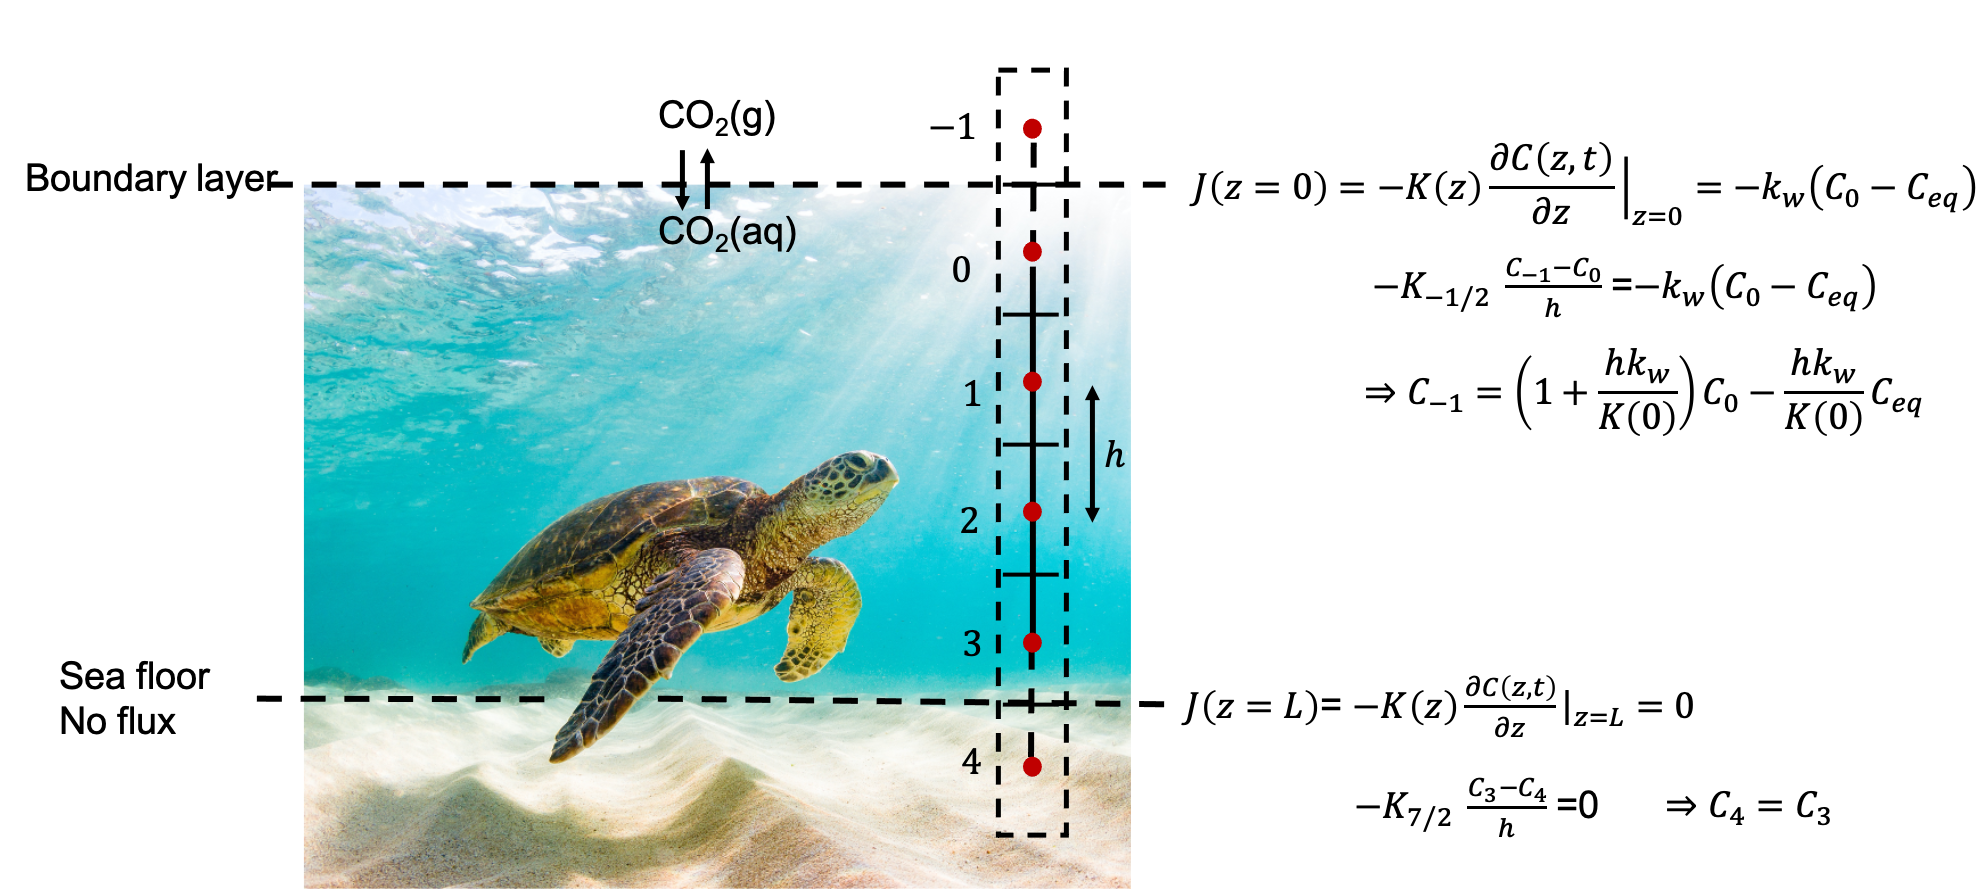
\includegraphics[width=1.0\linewidth]{fig-lin/co2_diff.png}}
  \caption{
  Discretization for diffusion of \co\ into an aquifer, including boundary conditions. \label{fig:lin:co2_diff}
  }
\end{figure}
%\clearpage % flush figures fig:lin:co2_diff

In the following we will assume that there are only four nodes ($i=0\ldots 3$) in the physical domain, and two ghost nodes $i=-1$, and $i=4$. There are many ways to attack this problem, but in the following we will borrow ideas from Finite Volume. Finite volume methods is a way of discretizing equations such that we \emph{conserve mass}. The diffusion equation as it is derived in figure~\ref{fig:nlin:heat}, express that the flux of something (heat, particles, etc) leaving the box surface minus the flux entering the surface of the box is equal to the rate of change of something inside the box. We can formulate this mathematically as:
\begin{equation}
\frac{\partial C(z,t)}{\partial t}\simeq\frac{1}{h}\left[\left.K(z)\frac{\partial C(z,t)}{\partial z}\right|_{i+1/2}
-\left.K(z)\frac{\partial C(z,t)}{\partial z}\right|_{i-1/2}\right]
\label{eq:lin:co2fv}
\end{equation}
The notation $i\pm1/2$, means that the flux is to be evaluated \emph{at the surface} of the box (i.e.~halfway between the red dots in figure~\ref{fig:lin:co2_diff}). $K(z)$ is the diffusion constant, and it is known everywhere, so this is simple to evaluate at the surface. The concentrations are only known at the center of each box, the red dots in figure~\ref{fig:lin:co2_diff}. The derivative of the concentration can be evaluated using the central difference formula (remember that the distance between the red dot and edge of the box is $h/2$), hence
\begin{equation}
\frac{C_i^{n+1}-C_i^n}{\Delta t}=\frac{1}{h}\left[K_{i+1/2}\frac{ C_{i+1}-C_{i}}{h}-K_{i-1/2}\frac{ C_{i}-C_{i-1}}{h}\right],
\label{eq:lin:co2fv2}
\end{equation}
notice that we have discretized the time derivative, and that we have introduced $n$ to indicate the time step. On the right hand side there are is no time indicated, it turns out that we have a choice to put time step $n$ or $n+1$ on the concentrations on the right hand side. If we put $n$ the scheme is said to be explicit, if we put $n+1$, the scheme is implicit. Implicit schemes are stable compared to explicit schemes, whereas explicit schemes has slightly higher numerical accuracy \shortinlinecomment{TO DO 1}{ show this! }{ show this! }. In general we can write
\begin{align}
\frac{C_i^{n+1}-C_i^n}{\Delta t}&=\frac{\theta}{h}\left[K_{i+1/2}
\frac{C^n_{i+1}-C^n_{i}}{h}-K_{i-1/2}\frac{C^n_{i}-C^n_{i-1}}{h}\right]\\ 
&+\frac{1-\theta}{h}\left[K_{i+1/2}
\frac{C_{i+1}^{n+1}-C_{i}^{n+1}}{h}-K_{i-1/2}\frac{ C_{i}^{n+1}-C_{i-1}^{n+1}}{h}\right],
\label{eq:lin:co2fv23}
\end{align}
hence if $\theta=1$ the scheme is explicit, if $\theta=0$ the scheme is implicit, and if $\theta=1/2$, the scheme is called the Crank-Nicolson method. The first and last boundary are special, let us first consider the $i=0$, this is where the sea is in contact with the \co\ in the atmosphere, and the flux is $k_w(C_0-C_{eq})$, hence
\begin{align}
\frac{C_0^{n+1}-C_0^n}{\Delta t}&=\frac{\theta}{h}\left[K_{i+1/2}
\frac{C^n_{1}-C^n_{0}}{h}-k_w(C_0^n-C_{eq}^n)\right]\\ 
&+\frac{1-\theta}{h}\left[K_{i+1/2}
\frac{C_{1}^{n+1}-C_{0}^{n+1}}{h}-k_w(C_0^{n+1}-C_{eq}^{n+1})\right].
\label{eq:lin:co2fv23b}
\end{align}
For the last block the flux is zero towards the seafloor, and equation (\ref{eq:lin:co2fv23}) can be written
\begin{align}
\frac{C_3^{n+1}-C_3^n}{\Delta t} & =\frac{\theta}{h}\left[-K_{5/2}\frac{C^n_{3}-C^n_{2}}{h}\right]\\ 
&+\frac{1-\theta}{h}\left[-K_{5/2}\frac{ C_{3}^{n+1}-C_{2}^{n+1}}{h}\right].
\label{eq:lin:co2fv23c}
\end{align}
For the blocks $i=1\ldots2$, we can collect all terms with $n+1$ on one side and terms with $n$ on the other side and rewrite equation (\ref{eq:lin:co2fv23})
\begin{align}
\left[1+(1-\theta)\right. &\left.\alpha(K_{i+1/2}+K_{i-1/2})\right]C_i^{n+1}\no\\ 
&-(1-\theta)\alpha K_{i+1/2}C_{i+1}^{n+1}
-(1-\theta)\alpha K_{i-1/2}C_{i-1}^{n+1} \no\\ 
=\left[1-\theta\right. &\left.\alpha(K_{i+1/2}+K_{i-1/2})\right]C_i^{n}\no\\ 
&+\theta\alpha K_{i+1/2}C_{i+1}^{n}
+\theta\alpha K_{i-1/2}C_{i-1}^{n}, 
\label{eq:lin:co2fv4}
\end{align}
where $\alpha\equiv\Delta t/h^2$.
Next, we want to write down the corresponding matrix equations for four grid nodes as indicated in figure~\ref{fig:lin:co2_diff}. Notice that we need to use the equations in figure~\ref{fig:lin:co2_diff}, for $C_{-1}$, and $C_4$. The left and right hand coefficient matrix $\mathbf{L}$, and $\mathbf{R}$ are given as
{\tiny
\begin{align}
\begin{pmatrix}
1+(1-\theta)\alpha(K_{1/2}+hk_w)&-(1-\theta)\alpha K_{1/2}&0&0\\ 
-(1-\theta)\alpha K_{1/2}&1+(1-\theta)\alpha(K_{3/2}+K_{1/2})&-(1-\theta)\alpha K_{3/2} &0\\ 
0&-(1-\theta)\alpha K_{3/2}&1+(1-\theta)\alpha(K_{5/2}+K_{3/2})&-(1-\theta)\alpha K_{5/2} \\ 
0&0&-(1-\theta)\alpha K_{5/2}&1+(1-\theta)\alpha K_{5/2}\no
\end{pmatrix},
\end{align}
}
{\tiny
\begin{align}
\begin{pmatrix}
1-\theta\alpha(K_{1/2}+hk_w)&+\theta\alpha K_{1/2}&0&0\\ 
\theta\alpha K_{1/2}&1-\theta\alpha(K_{3/2}+K_{1/2})&\theta\alpha K_{3/2} &0\\ 
0&\theta\alpha K_{3/2}&1-\theta\alpha(K_{5/2}+K_{3/2})&\theta\alpha K_{5/2} \\ 
0&0&\theta\alpha K_{5/2}&1-\theta\alpha K_{5/2}\no
\end{pmatrix},
\end{align}
}
respectively. Introducing $\mathbf{S}=\left[k_wC_{eq}\Delta t/h,0,0,0\right]^T$, we can finally write the diffusion equation (\ref{eq:lin:co2_diff}) as
\begin{equation}
\mathbf{L}\mathbf{C}^{n+1}=\mathbf{R}\mathbf{C}^n+\theta\mathbf{S}^n+(1-\theta)\mathbf{S}^{n+1}
\label{eq:lin:discdif}
\end{equation}

More stuff to do:
\begin{enumerate}
\item Assume zero flux over the air water interface ($k_w$=0), show from the equations above that if we start with a uniform concentration in the sea ($\mathbf{C}^n$=constant) that $\mathbf{C}^{n+1}$ does not change (as it should).

\item Assume that if the concentration at a specific time $n$ in the sea is equal to $\mathbf{C}_{eq}$ then the concentration stays constant at all later times

\item Add chemical reactions
\end{enumerate}

\noindent
% !split
\chapter{Optimization and nonlinear systems}
\label{ch:nlin}
% Contrary to linear equations, you will most likely find that the functions available in
% various Python library will \emph{not} cover your needs and in many cases fail to give you
% the correct solution. The reason for this is that the solution of a nonlinear equation # is greatly
% dependent on the starting point, and a combination of various techniques  must be used.

In this chapter we will cover some theory related to the solution of nonlinear equations, and introduce the most used methods. A nonlinear problem is represented as a single equation or a system of equations, where the response is not changing proportionally to the input.  Almost all physical systems are nonlinear, and one frequent use of the methods presented in this chapter is to determine model parameters by matching a nonlinear model to data. 

Numerical methods that is guaranteed to find a solution (if it exists) are called \emph{closed methods}, and \emph{open} other vise. In many cases the closed methods requires more iterations for well behaved functions than the open methods. For one dimensional problems we will cover: fixed point iteration, bisection, Newton's method, and the secant method.
For  multidimensional problems we will cover Newton-Rapson method, which is a direct extension of Newton's method in one
dimension, and the steepest decent. The main challenge is that there are (usually) more than one solution, the solution that
\emph{you} want for a specific problem is usually dictated by the underlying physics. If computational speed is not an issue, the
 method of choice is usually the bisection method. It is guaranteed to give an answer, but it might be slow. If speed is an issue, usually Newton's or the secant method will be the fastest (but it depends on the starting point). The secant method is sometimes preferred if the derivative of the function is costly to evaluate. Brents method is a method that combine the secant and bisection method (not covered), and is guaranteed to find a solution if the root is bracketed. 

In many practical, engineering, applications one usually implements some of the methods described below directly inside functions. This is because it is usually faster than calling a separate all purpose nonlinear solver, and that one usually has a very good idea of what a good starting point for the nonlinear solver is. 

\section{Nonlinear equations}
A nonlinear equation is simply an equation that is not linear. That means that when the variables changes the response is not changing proportional to the values of the variables. Solving a nonlinear equation always proceeds by \emph{iterations}, we start with one or several initial guesses and then search for the solution. In many cases we do not know beforehand if the equation actually has a solution, or multiple solutions. An example of a nonlinear problem is:
\begin{equation}
e^{-x}=x^2.
\label{eq:nlin:exp}
\end{equation}
Traditionally one collect all the terms on one side, to solve an equation of the form
\begin{equation}
f(x)=x^2-e^{-x}=0.
\label{eq:nlin:fx}
\end{equation}
In figure~\ref{fig:nlin:fx}, the solution is shown graphically. Note that in one case the solution is when the graph of $e^{-x}$, and $x^2$ intersect, whereas in the other case the root is located when $x^2-e^{-x}$ intersect the $x-$axis. 

\begin{figure}[!ht]  % fig:nlin:fx
  \centerline{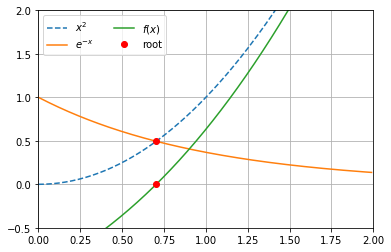
\includegraphics[width=0.5\linewidth]{fig-nlin/fx.png}}
  \caption{
  Notice that the root is located at the same place ($x=0.703467417$) \label{fig:nlin:fx}
  }
\end{figure}
%\clearpage % flush figures fig:nlin:fx

In the case of more than one unknown, or a set of equations that must be satisfied simultaneously, equation (\ref{eq:nlin:fx}) is replaced with a vector equation
\begin{equation}
\mathbf{f}(\mathbf{x})=\mathbf{0}.
\label{eq:nlin:fvec}
\end{equation}
Although this equation looks quite similar to equation (\ref{eq:nlin:fx}), this equation is \emph{much} harder to solve. The only methods we will cover is the Newton Rapson method, which is a very good method if a good starting point is given. If you have a multidimensional problem, the advice is to try Newton-Raphson, if this method fails you need to try more advanced method, see e.g.~\cite{press2001}.

\section{Example: van der Waals equation of state}
Before we begin with the numerical algorithms, let us consider an example: the van der Waals equation of state. The purpose is to illustrate some of the typical challenges. You are probably familiar with the ideal gas law:
\begin{equation}
P\nu=R_gT,
\label{eq:nlin:pvt}
\end{equation}
where $\nu=V/n$ is the molar volume of the gas, $P$ is the pressure, $V$ is the volume, $T$ is the temperature, $n$ is the number of moles of the gas, and $R_g$ is the ideal gas constant.  This equation is an example of an \emph{equation of state} (EOS), it relates $P$, $T$, and $\nu$. Thus if we know the pressure and temperature of the gas, we can calculate $\nu$. Equation (\ref{eq:nlin:pvt}) assumes that there are no interactions between the molecules in the gas. Clearly, this is too simplistic, and because of this one normally uses an EOS that better reflect the physical properties of the substance. A very famous EOS is the van der Waal EOS, which is a slight modification of equation (\ref{eq:nlin:pvt}):
\begin{equation}
\left(P+\frac{a}{\nu^2}\right)\left(\nu-b\right)=R_gT.
\label{eq:nlin:vdw}
\end{equation}
$a$ and $b$ are material constants that needs to be determined experimentally. This equation is \emph{not} used in industrial design, but most equations used in practice are based on equation (\ref{eq:nlin:vdw}). Multiplying equation (\ref{eq:nlin:vdw}) with $\nu^2$, we get a non linear equation that is cubic in the molar volume. It turns out that cubic EOS are a class of equations that are quite successful in modeling the behavior of real systems \cite{peng1976new}. However equation (\ref{eq:nlin:vdw}) is a good starting point for more complex and realistic equations.

It is common practice to rescale EOS with respect to the critical point. At the critical point we have [ref]:
\begin{align}
\left.\frac{\partial P}{\partial \nu}\right|_{T_c,P_c} &=0
\label{eq:nlin:crit1} \\ 
\left.\frac{\partial^2 P}{\partial \nu^2}\right|_{T_c,P_c} &=0
\label{eq:nlin:crit2} 
\end{align}
From equation (\ref{eq:nlin:crit1}),  (\ref{eq:nlin:crit2}), and (\ref{eq:nlin:vdw}), it follows:
\begin{equation}
\nu_c=3b\quad,P_c=\frac{a}{27b^2}\quad,R_gT_c=\frac{8a}{27b^2}.
\label{eq:nlin:crit3}
\end{equation}
Inserting these equations into equation (\ref{eq:nlin:vdw}), and defining the \emph{reduced} quantities $\hat{P}=P/P_c$, $\hat{T}=T/T_c$, $\hat{\nu}=\nu/\nu_c$, we get
\begin{equation}
\left(\hat{P}+\frac{3}{\hat{\nu}^2}\right)\left(3\hat{\nu}-1\right)=8\hat{T}.
\label{eq:nlin:vdwr}
\end{equation}

\begin{figure}[!ht]  % fig:nlin:vdw
  \centerline{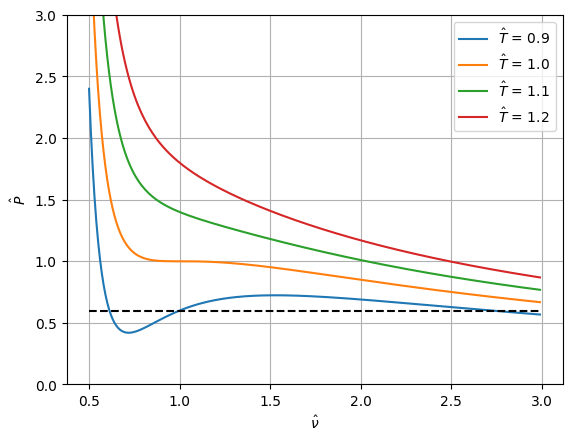
\includegraphics[width=1.0\linewidth]{fig-nlin/vdw.png}}
  \caption{
  van der Waal isotherms. \label{fig:nlin:vdw}
  }
\end{figure}
%\clearpage % flush figures fig:nlin:vdw

In figure~\ref{fig:nlin:vdw}, we have plotted the isotherms. Note that if $\hat{T}<1$ ($T<T_c$), there might be more than one solution for the molar volume. This is clearly unphysical and additional constraints are needed. For the curve $\hat{T}=0.9$, the dashed lined shows that for $\hat{P}=0.7$, there are three solutions. This is a typical behavior of the cubic EOS, and physically it corresponds to the saturated case, where the vapor and liquid phase co-exist. The left root is the liquid state and the right root is the vapor state. The root in the middle represents a meta stable state.



\begin{graybox2admon}[It never hurts to look at your function]
The example in figure~\ref{fig:nlin:vdw} illustrates some important points. Solving a nonlinear problem might be very easy in part of the parameter space (e.g.~when $T>T_c$ there are only one solution), but extremely hard in other part of the parameter space (e.g.~when $T<T_c$, where there are multiple solutions). However, much of the trick to find a solution is to choose a good starting point. When there are multiple solutions we need to start close to the physical solution.
\end{graybox2admon}




% --- begin exercise ---
\begin{doconceexercise}
\refstepcounter{doconceexercisecounter}

\exercisesection{Exercise \thedoconceexercisecounter: van der Waal EOS and CO$_2$}
                             

Use equation (\ref{eq:nlin:vdw}), and the parameters for CO$_2$: a=3.640 L$^2$bar/mol, and b=0.04267 L/mol, to test the van der Waal EOS in equation (\ref{eq:nlin:vdw}). Use that at 2 MPa and 100 $^\circ$C, CO$_2$ has a specific volume of 0.033586 m$^3$/kg.

% --- begin solution of exercise ---
\paragraph{Solution.}
The calculation is straight forward, but it is easy to get an error due to units. We will use SI units: a=0.3640 m$^6$Pa/mol, b=4.267$\cdot10^{-5}$ m$^3$/mol, $R$=8.314J/mol K.  The molar volume is obtained by multiplying by the molar weight of CO$_2$: $M_w$ = 44 g/mol, hence $\nu=1.478\cdot10^{-3}$m$^3$/mol. Using $P=RT/(\nu-b)-a/\nu^2=1.993$ MPa, or an error of $0.3\%$.

% --- end solution of exercise ---

\end{doconceexercise}
% --- end exercise ---

\section{Fixed-point iteration}
\index{fixed-point iteration}
A simple (but not always possible) way of solving a nonlinear equation is to reformulate the problem $f(x)=0$ to a problem of the form
\begin{equation}
x=g(x).
\label{eq:nlin:g}
\end{equation}
The algorithm for solving this equation is to guess at a starting point, $x_0$, evaluate $x_1=g(x_0)$, $x_2=g(x_1)$, and so on. In some circumstances we might end up at a stable point, where $x$ does not change. This point is termed a \emph{fixed point}.

Note that the form of $g(x)$ is not uniquely determined. For our function defined in equation (\ref{eq:nlin:exp}), we can solve for $x$ directly
\begin{equation}
x=e^{-x/2},
\label{eq:nlin:g2}
\end{equation}
or we could write:
\begin{equation}
x=x-x^2+e^{-x}.
\label{eq:nlin:g3}
\end{equation}
These functions are illustrated in figure~\ref{fig:nlin:fg}, by visual inspection they look very similar, but as we will show in the next exercise the convergence is quite different. 

\begin{figure}[!ht]  % fig:nlin:fg
  \centerline{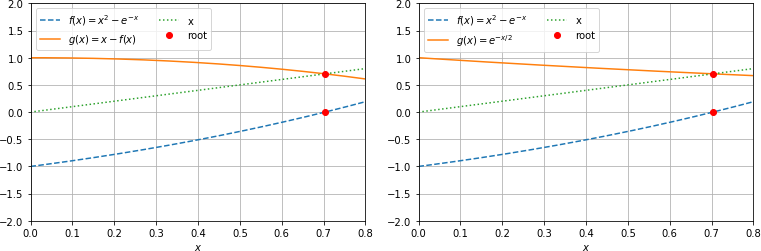
\includegraphics[width=1.0\linewidth]{fig-nlin/f_g_comb.png}}
  \caption{
  Two examples of iterative functions, that will give the same solution. \label{fig:nlin:fg}
  }
\end{figure}
%\clearpage % flush figures fig:nlin:fg

% --- begin exercise ---
\begin{doconceexercise}
\refstepcounter{doconceexercisecounter}

\exercisesection{Exercise \thedoconceexercisecounter: Implement the fixed point iteration}
                             

Write a Python function that utilizes the fixed point algorithm in the previous section, find the root of $f(x)=x^2-e^{-x}$. In one case use $g(x)=e^{-x/2}$, and in the other case use $g(x)=x-x^2+e^{-x}$. How many iterations does it take in each case?

% --- begin solution of exercise ---
\paragraph{Solution.}
Below is a straight forward (vanilla) implementation:























\begin{lstlisting}[language=python,style=blue1]
def iterative(x,g,prec=1e-8, MAXIT=1000):
    '''Approximate solution of x=g(x) by fixed point iterations.
    x : starting point for iterations 
    eps : desired precision
    Returns x when x does not change more than prec
    and number of iterations MAXIT are not exceeded
    '''
    eps = 1
    n=0
    while eps>prec and n < MAXIT:
        x_next = g(x)
        eps = np.abs(x-x_next)
        x = x_next
        n += 1
        if(np.isinf(x)):
            print('Quitting .. maybe bad starting point?')
            return x
    if (n<MAXIT):
        print('Found solution: ', x, ' After ', n, 'iterations')
    else:
        print('Max number of iterations exceeded')
    return x

\end{lstlisting}

If we start at $x=0$, it will take 174 iterations using $x-x^2+e^{-x}$ ($g(x)$) and only 19 for $e^{-x/2}$ ($h(x)$), the root is $x$=0.70346742.

% --- end solution of exercise ---

\end{doconceexercise}
% --- end exercise ---

% --- begin exercise ---
\begin{doconceexercise}
\refstepcounter{doconceexercisecounter}

\exercisesection{Exercise \thedoconceexercisecounter: Finding the molar volume from the van der Waal EOS by fixed point iteration}
                             

Extend the code above to take as argument the van der Waal EOS. For simplicity we will use the rescaled EOS in equation (\ref{eq:nlin:vdwr}). Show that for the reduced temperature, $\hat{T}$=1.2, and pressure, $\hat{P}$=1.5, the reduced molar volume $\hat{nu}$ is 1.3522091.

% --- begin solution of exercise ---
\paragraph{Solution.}
First we rewrite equation (\ref{eq:nlin:vdwr}) in a more useful form
\begin{equation}
\hat{\nu}=\frac{1}{3}(1+\frac{8\hat{T}}{\hat{P}+3/\hat{\nu}^2})
\label{eq:nlin:sp}
\end{equation}
The right hand side will play the same role as $g(x)$ above, where $x$ now is the reduced molar volume, and can be implemented in Python as:



\begin{lstlisting}[language=python,style=blue1]
def dvdwEOS(nu,t,p):
    return (1+8*t/(p+3/nu**2))/3

\end{lstlisting}

Note that this function requires the values of $\hat{P}$ and $\hat{T}$, in addition to $\hat{\nu}$ to return a value. Thus in order to use the fixed point iteration method implemented above, we need to pass arguments to our function. This can easily be achieved by taking advantage of Pythons \texttt{*args} functionality. By simply rewriting our implementation slightly:












\begin{lstlisting}[language=python,style=blue1]
def iterative(x,g,*args,prec=1e-8):
    MAX_ITER=1000
    eps = 1
    n=0
    while eps>prec and n < MAX_ITER:
        x_next = g(x,*args)
        eps = np.abs(x-x_next)
        x = x_next
        n += 1
    print('Number of iterations: ', n)
    return x

\end{lstlisting}

We can find the root by calling the function as:


\begin{lstlisting}[language=python,style=blue1bar]
iterative(1,dvdwEOS,1.2,1.5)

\end{lstlisting}

The program returns the correct solution after 71 iterations.

% --- end solution of exercise ---

\end{doconceexercise}
% --- end exercise ---

\subsection{When does the fixed point method fail?}
\label{sec:nlin:fp}
If we replace $e^{-x}$ with $e^{1-x^2}$ in equation (\ref{eq:nlin:g3}), our method will not give a solution. You can easily verify that the $x=1$ is a solution, so why does our method fail? To investigate this in a bit more detail, we turn to Taylors formula (once again). Assume that the root is located at $x^*$, and our guess is $x_k$, then the next $x$-value will be
\begin{equation}
x_{k+1}=g(x_0)=g(x^*)+g^\prime(x^*)(x_k-x^*)+\cdots
\label{eq:nlin:t1}
\end{equation}
The true solution is $x^*$, hence $x^*=f(x^*)$, and we can write
\begin{equation}
x_{k+1}-x^*=g^\prime(x^*)(x_k-x^*),
\label{eq:nlin:t2}
\end{equation}
where we have neglected higher order terms. The point is: at each iteration we want the distance $x_1-x^*$ to decrease, i.e.~to be smaller than $x_0-x^*$. This can only be achieved if
\begin{equation}
|g^\prime(x^*)|<1. 
\label{eq:nlin:fpi}
\end{equation}
In our example above we saw that if $g(x)=x-x^2+e^{-x}$, we used 172 iterations and only 19 iterations if we replaced $g(x)$ with $h(x)=e^{-x/2}$ to converge to the \emph{same} root $x$=0.70346742. We can now understand this, because $g^\prime(x)=1-2x-e^{-x}$ and $g(x^*)\simeq-0.90$, whereas $h^\prime(x)=-e^{-x/2}/2$, and $h^\prime(x^*)\simeq0.35$. We expect the number of iterations, $n$, needed to reach a certain precision, $\varepsilon$, to scale as
\begin{equation}
|g^\prime(x^*)|^n=\varepsilon.
\label{eq:nlin:scale}
\end{equation}
We expect to use $\log|h^\prime(x^*)|/\log|g^\prime(x^*)|\simeq10$ more iterations using $g(x)$ compared to $h(x)$, which is close to the observed value of 172/19$\simeq 9$.
\subsection{What to do when the fixed point method fails}
As discussed in \cite{newman2013}, there might be an elegant solution whenever $|g^\prime(x^*)|>1$. If it is possible to invert the $g(x)$, we can show that the derivative of the inverse function
$ { g^\prime }^{-1} (x^*)  = 1/g^\prime (x^*) $. Why is this useful? Because if $x^*=g(x^*)$ is the solution we are searching for, then this is equivalent to $x^*={g}^{-1}(x^*)$ \emph{if and only if} we can invert $g(x)$. Note that in many cases it is not possible to invert $g(x)$. Let us first show that $ { g^\prime }^{-1} (x^*)  = 1/g^\prime (x^*) $. For simplicity write
\begin{equation}
y = g(x)\Leftarrow x=g^{-1}(y),
\end{equation}
taking the derivative with respect to x gives
\begin{align}
\frac{d}{dx}g^{-1}(y)&=\frac{dx}{dx}=1,\label{eq:nlin:fpi1}\\ 
\frac{dg^{-1}(y)}{dy}\frac{dy}{dx}&=\frac{dx}{dx}=1,\label{eq:nlin:fpi2}\\ 
\frac{dg^{-1}(y)}{dy}&=\frac{1}{\frac{dy}{dx}}=\frac{1}{g^{\prime}(x)}
=\frac{1}{g^{\prime}(g^{-1}(y))}.\label{eq:nlin:fpi3}
\end{align}
Going from equation (\ref{eq:nlin:fpi1}) to (\ref{eq:nlin:fpi2}), we have used the chain rule. Equation (\ref{eq:nlin:fpi3}) is general, let us now specify to our fixed point iteration. Then we can use $x^*=g(x^*)=y^*$, and $x^*=g^{-1}(y^*)=g^{-1}(x^*)$ hence we can write the last equation as
\begin{equation}
\frac{d}{dx}g^{-1}(x^*)=\frac{1}{g^{\prime}(x^*)}.
\label{eq:nlin:fpif}
\end{equation}

% --- begin exercise ---
\begin{doconceexercise}
\refstepcounter{doconceexercisecounter}

\exercisesection{Exercise \thedoconceexercisecounter: Solve $x=e^{1-x^2}$ using fixed point iteration}
                             

The solution to $x=e^{1-x^2}$ is clearly $x=1$.

\begin{itemize}
\item First try the fixed point method using $g(x)=e^{1-x^2}$ to find the root $x=1$. Try to start very close to the true solution $x=1$. What is the value of $g^\prime(x^*)$?

\item Next, invert $g(x)$, what is the derivative of $g^{-1}(x^*)$? Try the fixed point method using $g^{-1}(x^*)$
\end{itemize}

\noindent
% --- begin solution of exercise ---
\paragraph{Solution.}
First, we calculate the derivative of $g(x)$, $g^\prime(x)=-2xe^{1-x^2}$, hence $g^\prime(x^*)=-2$ and $|g^\prime(x^*)|>1$. This is an unstable fixed point, and if we start a little bit off from this point we will spiral away from it.

Inverting $y=g(x)$ gives us $ g^{-1} (y)=\sqrt{1-\ln y}$. Note that $y^*=x^*=1$ is a solution to this equation as it should be. The derivative is
\begin{equation}
{g^{-1}}^\prime(y)=-\frac{1}{2\sqrt{1-\ln y}},
\end{equation}
and $ {g^{-1}}^\prime(y^*)=-1/2 $.
It takes about 30 iterations to reach the correct solution $y^*=1$, when the starting point is $y=0$.

% --- end solution of exercise ---

\end{doconceexercise}
% --- end exercise ---

\section{Rate of convergence}
\index{rate of convergence}
The rate of convergence is the speed at which a \emph{convergent} sequence approach the limit. Assume that our sequence $x_{k}$ converges to the number $x^*$, the sequence is said to \emph{converge linearly} to $x^*$ if there exists a number $\mu\in<0,1>$, such that
\begin{equation}
\lim_{k\to\infty}=\frac{|x_{k+1}-x^*|}{|x_k-x^*|}=\mu
\label{eq:nlin:linconv}
\end{equation}
Inserting equation (\ref{eq:nlin:t2}) in equation (\ref{eq:nlin:linconv}), we get:
\begin{equation}
\lim_{k\to\infty}=\frac{|x_{k+1}-x_k|}{x_k-x^*}
=\frac{|g^\prime(x^*)(x_k-x^*)|}{|x_k-x^*|}=|g^\prime(x^*)|.
\label{eq:nlin:ling}
\end{equation}
Hence the fixed point iteration is expected to converge \emph{linearly} to the correct solution. The definition in equation (\ref{eq:nlin:linconv}), can be extended to include the definition of quadratic, cubic, etc. convergence:
\begin{equation}
\lim_{k\to\infty}=\frac{|x_{k+1}-x^*|}{|x_k-x^*|^q}=\mu.
\label{eq:nlin:qconv}
\end{equation}
If $q=2$ the convergence is said to be quadratic and so on.

\section{The bisection method}
\index{bisection method}
The idea behind bisection is that the root is bracketed, i.e.~that there exists two points $a$ and $b$, such that $f(a)\cdot f(b)<0$. In practice it might be a challenge to find these two points. However, if you know that the function has a only root between two values, and that speed is not a big issue this method guarantees that the root will be found within a finite number of steps. The basic idea behind the method is to divide the interval into two (i.e.~bisecting the interval). The method only works if the function is continuous on the interval. 

\begin{figure}[!ht]  % fig:nlin:bisection
  \centerline{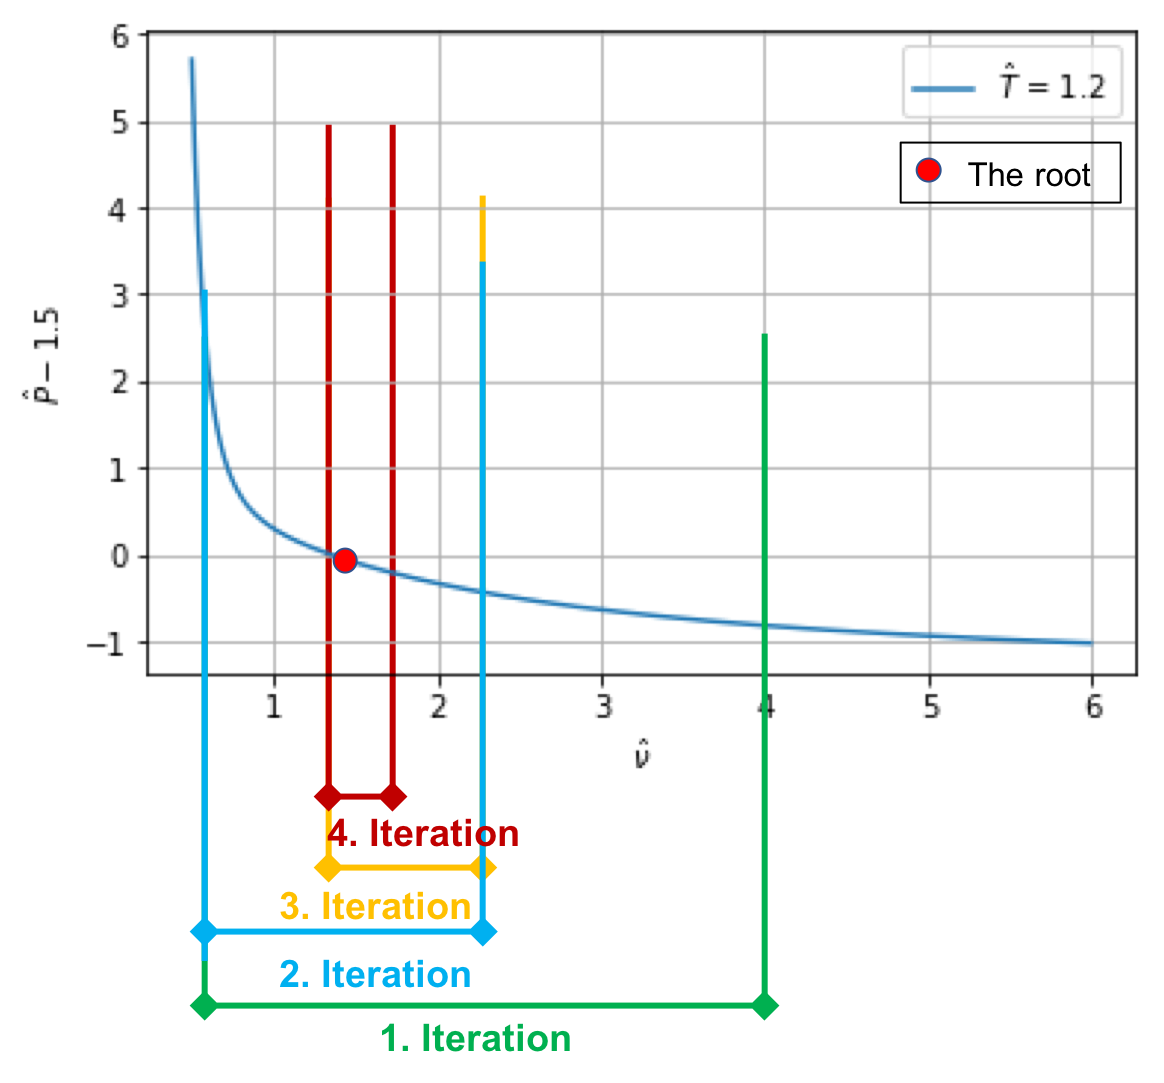
\includegraphics[width=1.0\linewidth]{fig-nlin/bisection.png}}
  \caption{
  Illustration of the bisection method for the van der Waal EOS. \label{fig:nlin:bisection}
  }
\end{figure}
%\clearpage % flush figures fig:nlin:bisection

The algorithm is as follows:
\begin{itemize}
\item Test if $f(a)\cdot f(b)<0$, if not return an error message

\item Calculate the midpoint $c=(a+b)/2$. If $f(a)\cdot f(c)<0$ the root is in the interval $[a,c]$, else the root is in the interval $[c,b]$

\item Half the interval, and test in which interval the root lies, and continue until a convergence criterion.
\end{itemize}

\noindent
In figure~\ref{fig:nlin:bisection}, there is a graphical illustration.
Below is an implementation of the bisection method.





































\begin{lstlisting}[language=python,style=blue1]
def bisection(f,a,b,PREC=1e-8,MAXIT=100):
    '''Approximate solution of f(x)=0 on interval [a,b] by bisection.

    f   : f(x)=0.
    a,b : brackets the root f(a)*f(b) has to be negative 
    PREC: desired precision
    
    Returns the midpoint when it is closer than eps to the root, 
    unless MAXIT are not exceeded
    '''
    if f(a)*f(b) > 0:
        print('You need to bracket the root, f(a)*f(b) >= 0')
        return None
    prec=10*PREC
    c = 0.5*(a + b)
    for n in range(MAXIT):
        c_old = c 
        fc = f(c)
        if fc == 0:
            print('Found exact solution ', c, 
                    ' after ', n, 'iterations' )
            return c
        if f(a)*fc < 0:
            b = c
        else:
            a = c
        c = 0.5*(a+b)
        prec=np.abs(c_old-c)
    if n<MAXIT-1:
        print('Found solution ', c,' after ', n, 'iterations' )
        return c
    else:
        print('Max number of iterations: ', MAXIT, ' reached.') 
        print('Try to increase MAXIT')
        print('Returning best guess, value of function is: ', fc)
    return c

\end{lstlisting}




\begin{graybox2admon}[Warnings]
Note that the implementation of the bisection algorithm is only a few lines of code, and most of the code is to give warnings to the user. In this case it is important to do additional checking, and give the user warnings. If $f(c)$=0, then we must stop and return the exact solution. If we only test if $f(a)\cdot f(c)$ is greater or lower than zero the algorithm would fail.
\end{graybox2admon}




\subsection{Rate of convergence}
\index{rate of convergence}
If $c_n$ is the midpoint after $n$ steps, the difference between the solution $x^*$ and $c_n$ is
\begin{equation}
|c_n-x^*| \le \frac{|b-a|}{2^n}
\label{eq:nlin:bisec}
\end{equation}
Using our previous definition in equation (\ref{eq:nlin:qconv}), we find that
\begin{equation}
\lim_{k\to\infty}=\frac{|c_{k+1}-x^*|}{|c_k-x^*|}\le\frac{|b-a|/2^{n+1}}{|b-a|/2^n}=\frac{1}{2},
\label{eq:nlin:bsc1}
\end{equation}
hence the bisection method converges linearly.
\section{Newton's method}
\index{Newtons method}
Newtons method is one of the most used methods. If it converges, it converges quadratically to the correct solution. The drawback is that contrary to the bisection method it may fail if a bad starting point is given. Newtons method for finding the root of a function $f(x)=0$ is illustrated in figure~\ref{fig:nlin:newton}. The main idea is to use more information about the function in the search of the root. In this case we want to find the point where the tangent of the function in $x_k$ intersect the $x-$axis, and take that as our next point, $x_{k+1}$. 

\begin{figure}[!ht]  % fig:nlin:newton
  \centerline{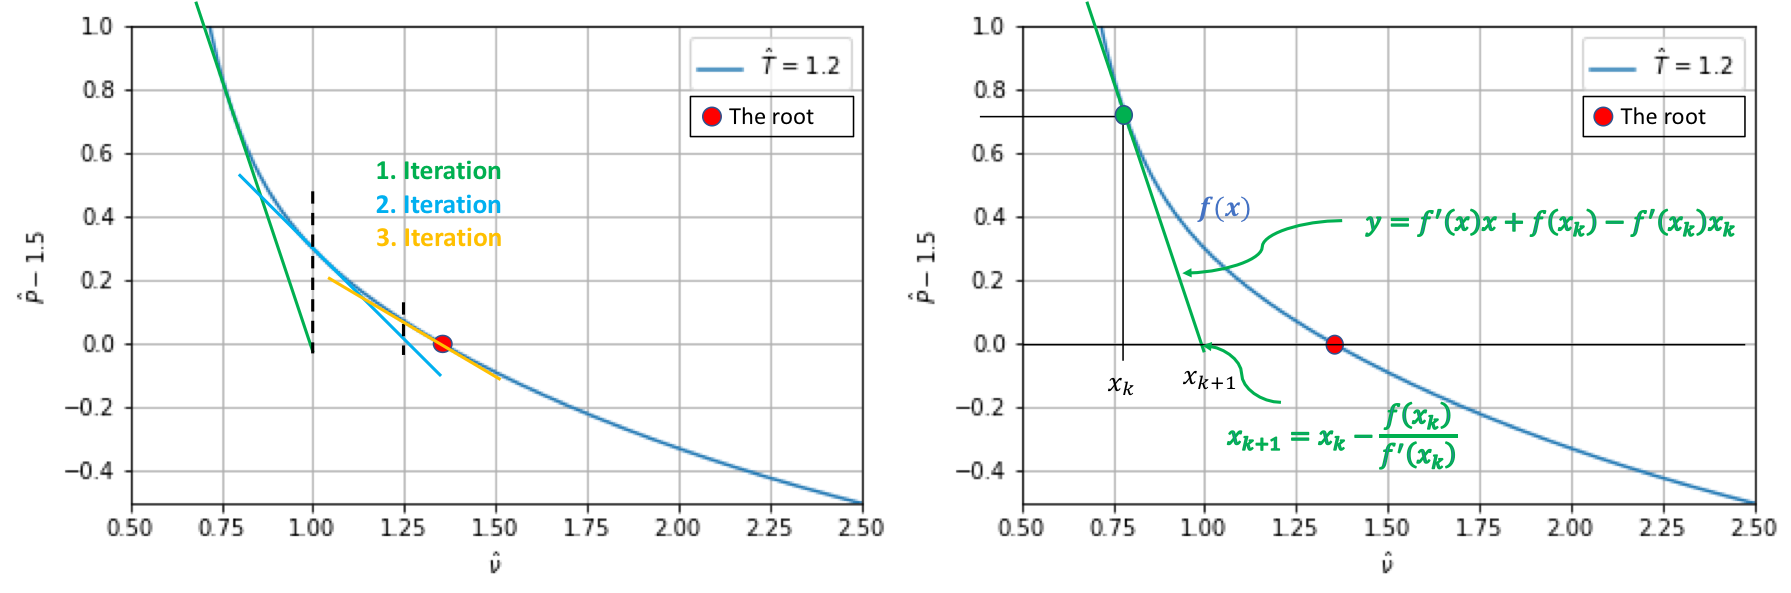
\includegraphics[width=1.0\linewidth]{fig-nlin/newton_comb.png}}
  \caption{
  Illustration of Newtons method for the van der Waals EOS.\label{fig:nlin:newton}
  }
\end{figure}
%\clearpage % flush figures fig:nlin:newton

We can easily derive the algorithm by finding the formula for the tangent line. Using $y=ax+b$ for the tangent line, we immediately know that $a=f^\prime(x_k)$. $b$ can be found as we know that the line intersects $(x_k,f(x_k))$: $f(x_k)=f^\prime(x_k)x_k+b$, hence the equation for the tangent line is $y=f^\prime(x_k)x+f(x_k)-f^\prime(x_k)x_k$. The next point is located where $y$ crosses the $x$-axis, hence $0=f^\prime(x_k)x_{k+1}+f(x_k)-f^\prime(x_k)x_k$. Rearranging this equation, we can write Newtons method in the standard form
\begin{equation}
x_{k+1}=x_k-\frac{f(x_k)}{f^\prime(x_k)}.
\label{eq:nlin:newton}
\end{equation}
Note that the derivative of $f(x)$ enters in equation (\ref{eq:nlin:newton}), which means that if our function has a extremal value in our search domain, Newtons method most likely will fail. In particular $x_1$, and $x_4$ in the figure to the right in figure~\ref{fig:nlin:newton2} are bad starting point for Newtons method.

\begin{figure}[!ht]  % fig:nlin:newton2
  \centerline{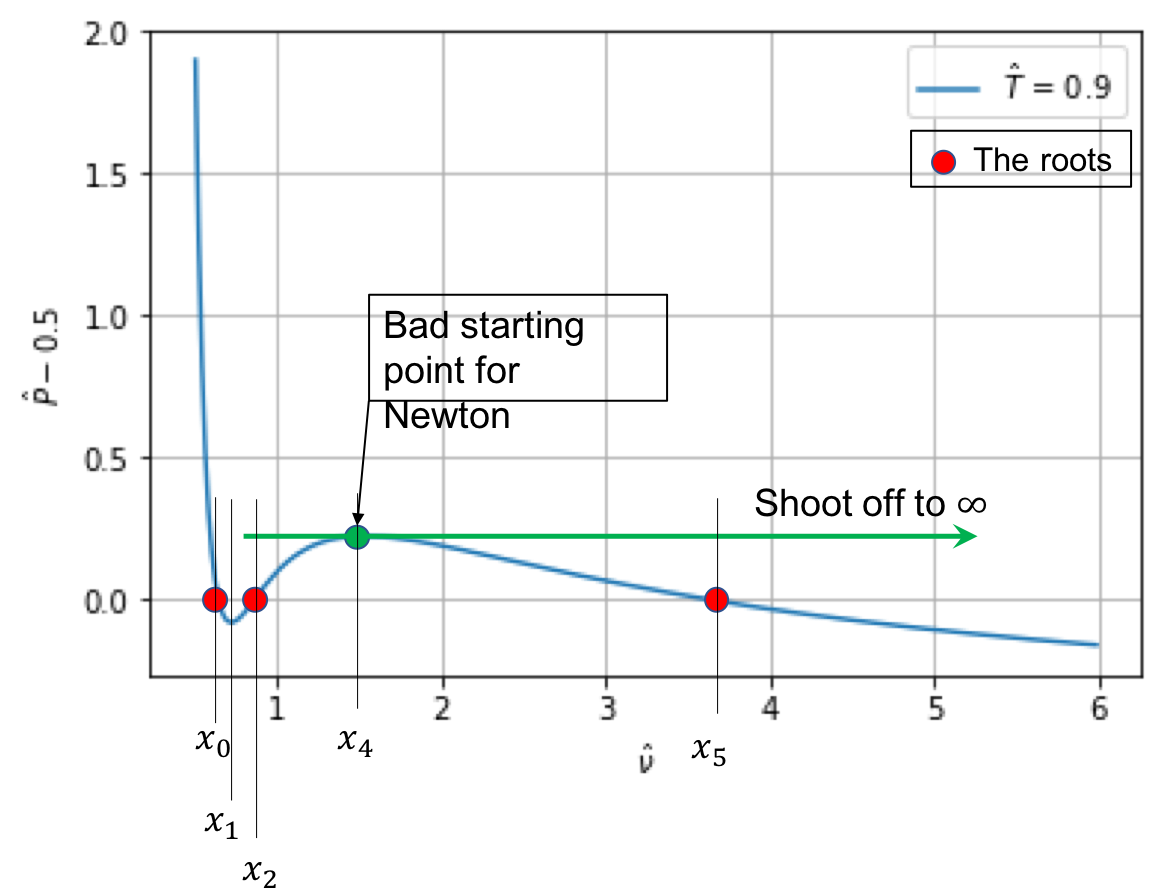
\includegraphics[width=1.0\linewidth]{fig-nlin/newton2.png}}
  \caption{
  Illustration of some of the possible challenges with Newtons method. Note that if the derivative is zero somewhere in the search interval, Newtons method will fail. \label{fig:nlin:newton2}
  }
\end{figure}
%\clearpage % flush figures fig:nlin:newton2

An implementation is shown below.

























\begin{lstlisting}[language=python,style=blue1]
def newton(f,x, prec=1e-8,MAXIT=500):
    '''Approximate solution of f(x)=0 by Newtons method.
    The derivative of the function is calculated numerically
    f   : f(x)=0.
    x   : starting point  
    eps : desired precision
    
    Returns x when it is closer than eps to the root, 
    unless MAX_ITERATIONS are not exceeded
    '''
    MAX_ITERATIONS=MAXIT
    x_old = x
    h     = 1e-4
    for n in range(MAX_ITERATIONS):
        x_new = x_old - 2*h*f(x_old)/(f(x_old+h)-f(x_old-h))
        if(abs(x_new-x_old)<prec):
            print('Found solution:', x_new, 
                  ', after:', n, 'iterations.' )
            return x_new
        x_old=x_new
    print('Max number of iterations: ', MAXIT, ' reached.') 
    print('Try to increase MAXIT or decrease prec')
    print('Returning best guess, value of function is: ', f(x_new))
    return x_new

\end{lstlisting}


Comparing figure~\ref{fig:nlin:bisection} and~\ref{fig:nlin:newton}, you immediately get the sense that Newtons method converges faster, and indeed it does. 

\subsection{Rate of convergence}
\index{Newtons method, rate of convergence}
 Newtons method is similar to the fixed point method, but where we do not use $g(x)=x-f(x)$, but $g(x)=x-\frac{f(x)}{f^\prime(x)}$. We will now analyze Newtons method, using the same approach as in section~\ref{sec:nlin:fp}. First we expand $g(x)$ around the root $x^*$
\begin{equation}
x_{k+1}=g(x_k)=g(x^*)+g^\prime(x^*)(x_k-x^*)+\frac{1}{2}g^{\prime\prime}(x^*)(x_k-x^*)^2,
\label{eq:nlin:nsec}
\end{equation}
where we have skipped all higher order terms. You can easily verify that
\begin{align}
g^\prime(x) &=\frac{f^{\prime\prime}(x)f(x)}{f^\prime(x)^2}
\label{eq:nlin:gn2} \\ 
g^{\prime\prime}(x) &=\frac{(f^{\prime\prime\prime}(x)f^\prime(x)-2f^{\prime\prime}(x)^2f^\prime(x))f(x)
+f^{\prime\prime}(x)f^\prime(x)^2}{f^\prime(x)^4}.
\label{eq:nlin:gn3}
\end{align}
$x^*$ is a solution, hence $f(x^*)=0$, we then find from equation (\ref{eq:nlin:gn2}) and (\ref{eq:nlin:gn3}) that $g^\prime(x^*)=0$, and $g^{\prime\prime}(x^*)=f^{\prime\prime}(x^*)/f^{\prime}(x^*)^2$. Thus from equation (\ref{eq:nlin:nsec}) we get
\begin{equation}
x_{k+1}=x^*+\frac{1}{2}\frac{f^{\prime\prime}(x^*)}{f^{\prime}(x^*)^2}(x_k-x^*)^2,
\label{eq:nlin:nsecn}
\end{equation}
or equivalently:
\begin{equation}
\frac{x_{k+1}-x^*}{(x-x^*)^2}=\frac{1}{2}\frac{f^{\prime\prime}(x^*)}{f^{\prime}(x^*)^2}.
\label{eq:nlin:nsecn2}
\end{equation}
The denominator has a power of two, and hence Newtons method is \emph{quadratic} convergent (assuming that the sequence $x_{k+1}$ is a convergent sequence). Note that it also follows from the analyses above that Newtons method will fail if the derivative at the root, $f^\prime(x^*)$, is zero.

% --- begin exercise ---
\begin{doconceexercise}
\refstepcounter{doconceexercisecounter}

\exercisesection{Exercise \thedoconceexercisecounter: Compare Newtons, Bisection and the Fixed Point method}
                             

Find the root of $f(x)=x^2-e^{-x}$ using bisection, fixed point,  and Newtons method, start at $x=0$. How many iterations do you need to use reach a precision of $10^{-8}$? What happens if you widen the search domain or start further away from the root?

% --- begin solution of exercise ---
\paragraph{Solution.}
The root is located at $x^*=0.70346742$.
\begin{itemize}
\item Fixed point method: we saw earlier that using $g(x)=x-f(x)$ used 174 iterations, and $g(x)=\sqrt{x^2-f(x)}$ used 19 iterations. If we start at $x=-100$, $g(x)=x-f(x)$ fails, and  $g(x)=\sqrt{x^2-f(x)}$ uses only 21 iterations, and at $x=100$ we use 20 iterations.

\item Bisection method: it use 25 iterations for $a=0$, and $b=1$ (implementation shown earlier in the chapter). Choosing $a=-b=-100$ we use 33 iterations.

\item Newtons method: it use only 5 function evaluations (implementation above) starting at  $x=0$. Starting at $x=-100$, it uses 106 iterations. Newtons method is slow in this case because the function is very steep around the starting point, see figure~\ref{fig:nlin:newton_bad}. Starting at $x=100$, we only use 10 iterations.
\end{itemize}

\noindent
\begin{figure}[!ht]  % fig:nlin:newton_bad
  \centerline{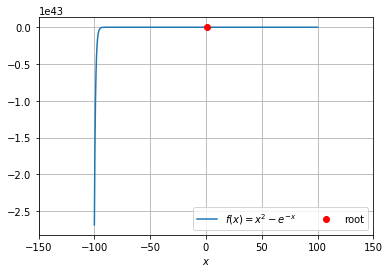
\includegraphics[width=1.0\linewidth]{fig-nlin/newton_bad.png}}
  \caption{
  Newtons method performs poorly far away due to the shape of the function close to $x=-100$, bisection performs much better while the fixed point method fails. \label{fig:nlin:newton_bad}
  }
\end{figure}
%\clearpage % flush figures fig:nlin:newton_bad



\begin{graybox2admon}[A good starting point is crucial]
Note that it is not given which method is best, but if we are ''close'' to the root Newtons method is usually superior. If we are far away, other methods might work better. In many cases one uses a more stable method far away from the root, and then ''polish up'' the root by a couple of Newton iterations \cite{press2001}. See also Brents method which combines bisection and linear interpolation (secant method) \cite{press2001}.
\end{graybox2admon}




% --- end solution of exercise ---

\end{doconceexercise}
% --- end exercise ---

\section{Secant method}
\index{secant method}
The Newtons method is very good if you can choose a good starting point, and you can give in an analytical formula for the derivative. In some cases it is not possible to calculate the derivative analytically, then a very good method of choice is the secant method. It can be derived by simply replacing the derivative in Newtons method by the finite difference approximation
\begin{equation}
f^\prime(x_k)\to \frac{f(x_k)-f(x_{k-1})}{x_k-x_{k-1}}.
\label{eq:nlin:sec1}
\end{equation}
Inserting this equation into equation (\ref{eq:nlin:newton}), we get
\begin{align}
x_{k+1}&=x_k-f(x_k)\frac{x_k-x_{k-1}}{f(x_k)-f(x_{k-1})}\no\\ 
       &=\frac{x_{k-1}f(x_k)-x_kf(x_{k-1})}{f(x_k)-f(x_{k-1})}. \label{eq:nlin:sec2}
\end{align}
For a graphical illustration see figure~\ref{fig:nlin:secant}

\begin{figure}[!ht]  % fig:nlin:secant
  \centerline{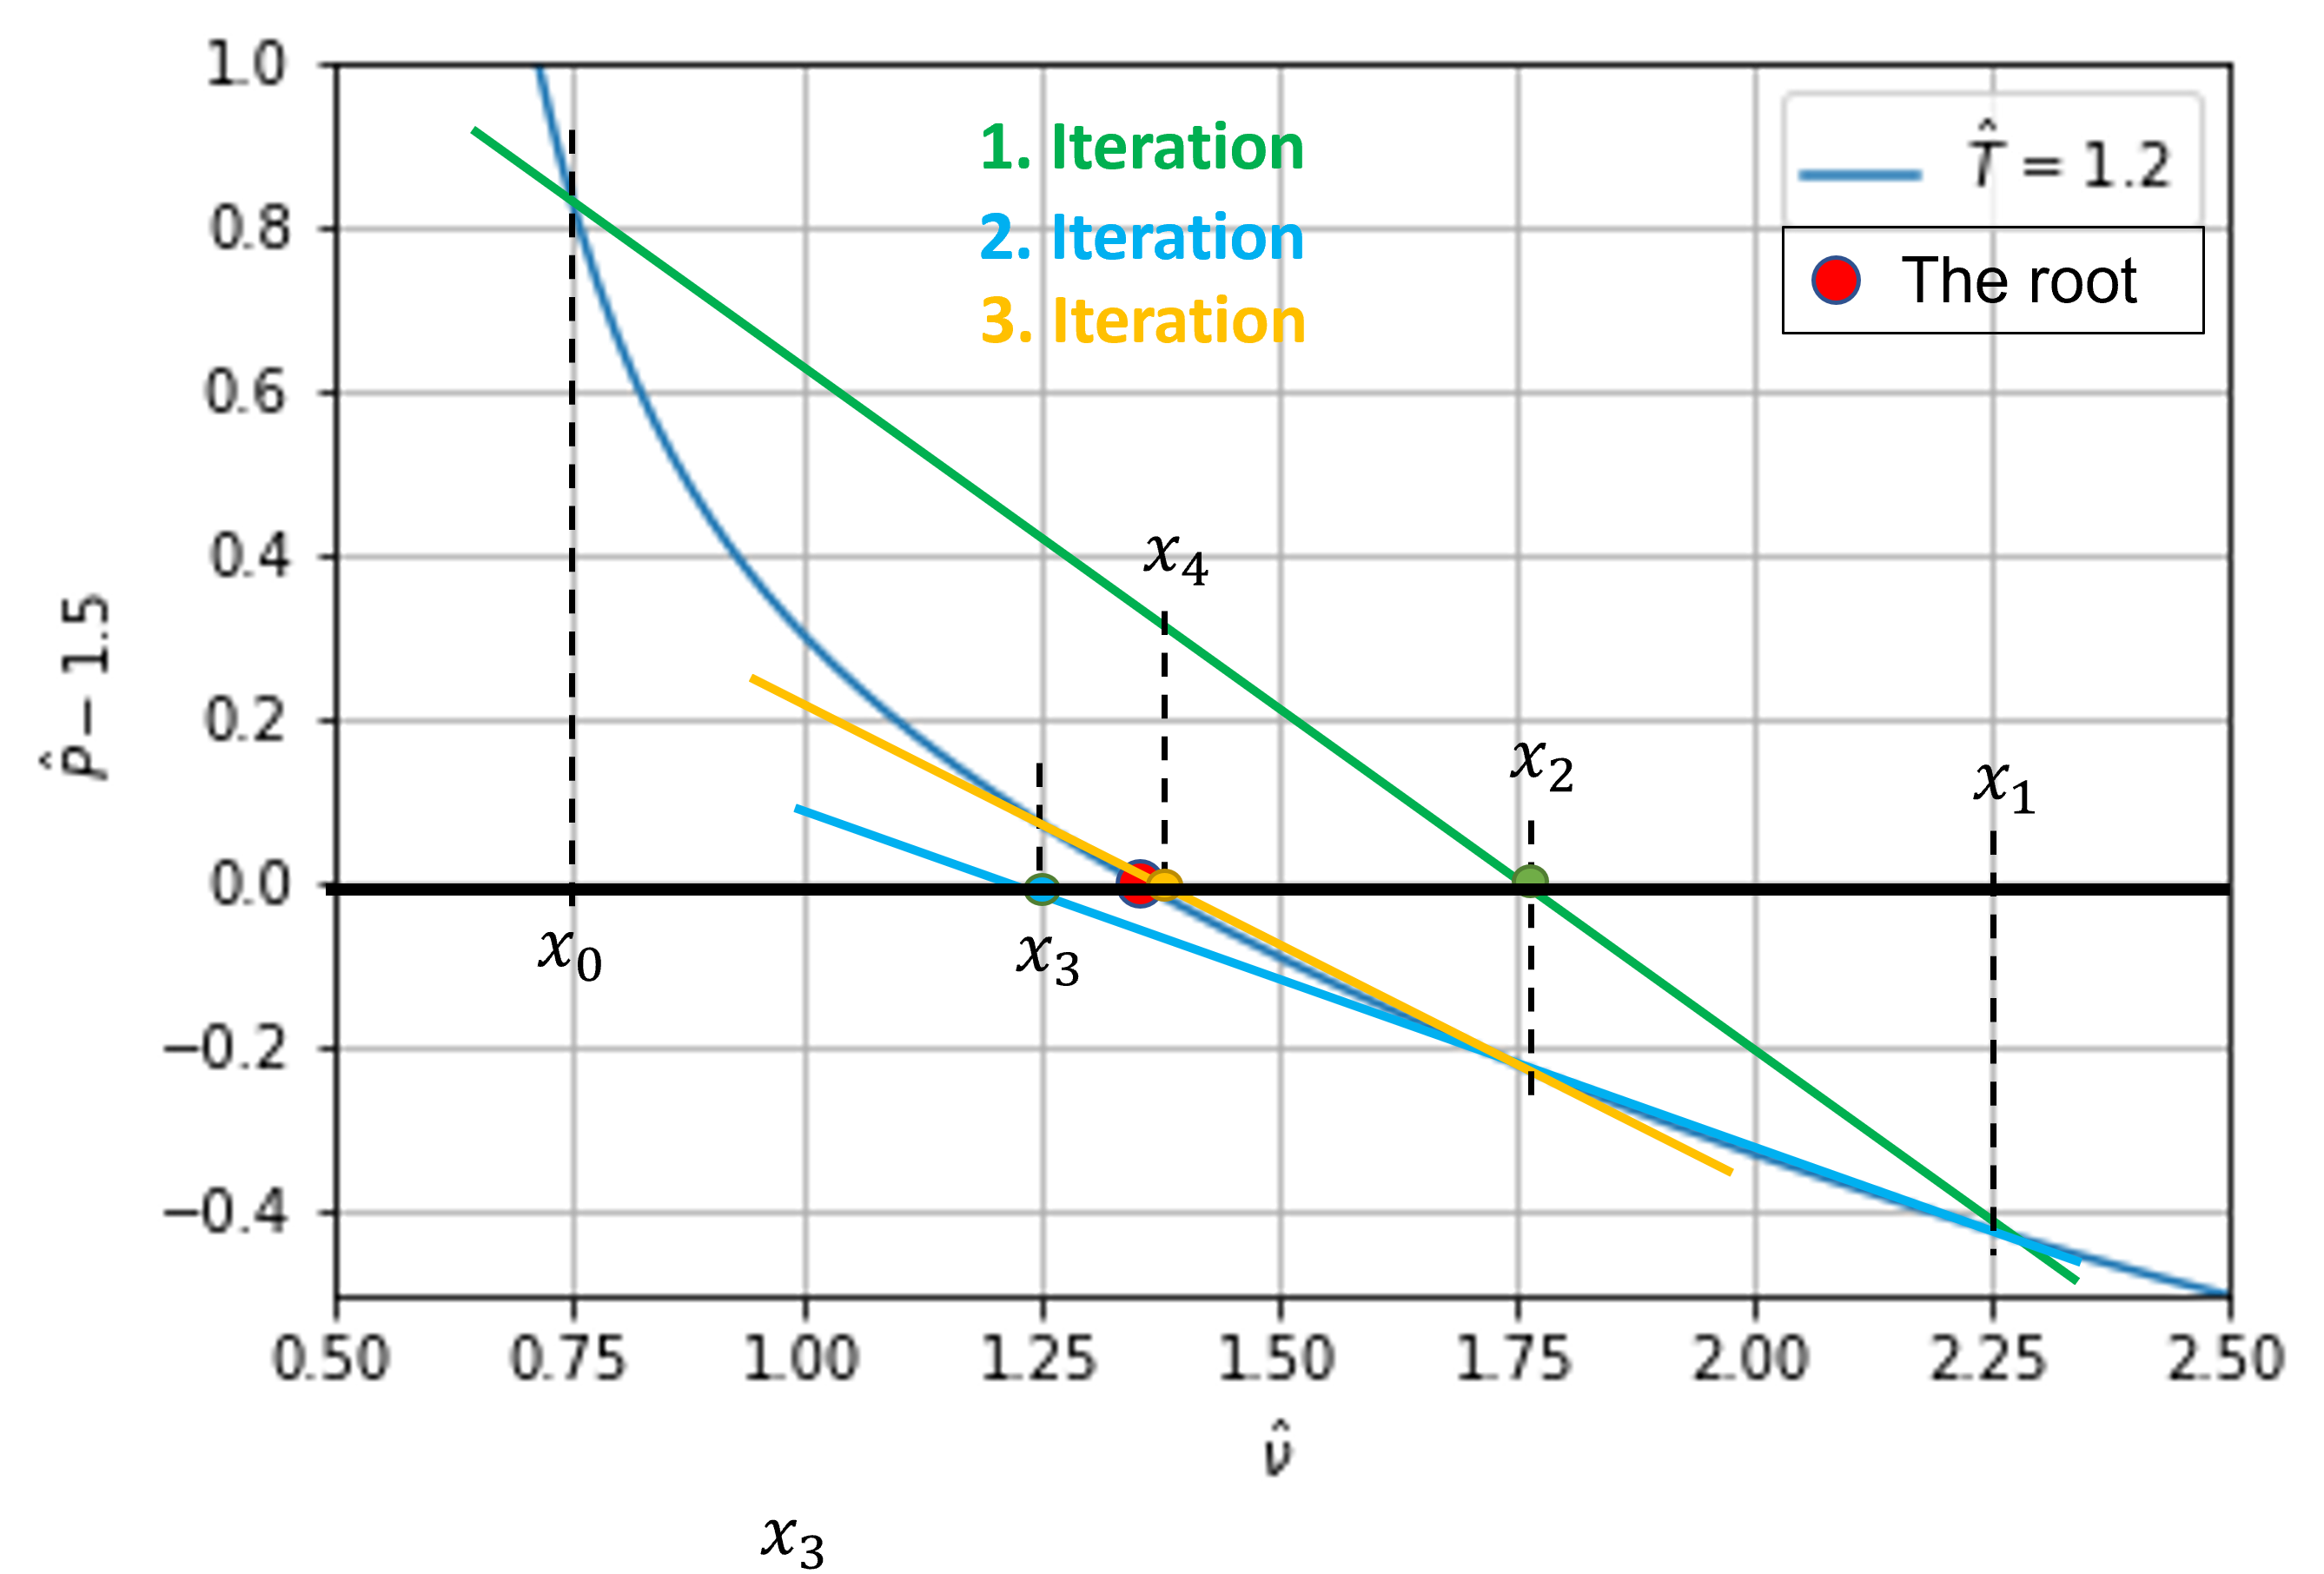
\includegraphics[width=1.0\linewidth]{fig-nlin/secant.png}}
  \caption{
  A graphical illustration of the secant method. Note that the starting points $x_0$ and $x_1$ do not need to be close. The next point is where the (secant) line crosses the $x$-axis. \label{fig:nlin:secant}
  }
\end{figure}
%\clearpage % flush figures fig:nlin:secant

\subsection{Rate of convergence}
\index{secant method, rate of convergence}
The derivation of the rate of convergence for the secant method is a bit more involved. To simplify the notation we introduce the notation $\varepsilon_k\equiv x_k-x^*$, where $x^*$ is the exact solution. Subtracting $x^*$ from each side of equation (\ref{eq:nlin:sec2}) we get
\begin{align}
\varepsilon_{k+1}&=x_{k+1}-x^*=\frac{x_{k-1}f(x_k)-x_kf(x_{k-1})}{f(x_k)-f(x_{k-1})}-x^*, \no\\ 
\varepsilon_{k+1}&=\frac{\varepsilon_{k-1}f(x_k)-\varepsilon_k f(x_{k-1})}{f(x_k)-f(x_{k-1})},
\label{eq:nlin:sec3}
\end{align}
we now make a Taylor expansion of $f(x_k)$ and $f(x_{k-1})$ about the root $x^*$
\begin{align}
f(x_k) &=f(x^*)+f^\prime(x^*)(x_k-x^*)+\frac{1}{2}f^{\prime\prime}(x^*)(x_k-x^*)^2+\cdots ,\no\\ 
       &=f^\prime(x^*)\varepsilon_k+\frac{1}{2}f^{\prime\prime}(x^*)\varepsilon_k^2+\cdots .\\ 
f(x_{k-1}) &=f(x^*)+f^\prime(x^*)(x_{k-1}-x^*)+\frac{1}{2}f^{\prime\prime}(x^*)(x_{k-1}-x^*)^2+\cdots,\no\\ 
       &=f^\prime(x^*)\varepsilon_{k-1}+\frac{1}{2}f^{\prime\prime}(x^*)\varepsilon_{k-1}^2+\cdots ,
\end{align}
where we have used the fact that $f(x^*)=0$. Inserting these equations into equation (\ref{eq:nlin:sec3}) and neglecting terms of order $\varepsilon_k^3$ we get
\begin{align}
\varepsilon_{k+1}&=\frac{\varepsilon_{k-1}\left[f^\prime(x^*)\varepsilon_k+\frac{1}{2}f^{\prime\prime}(x^*)\varepsilon_k^2\right] -\varepsilon_k\left[ f^\prime(x^*)\varepsilon_{k-1}+\frac{1}{2}f^{\prime\prime}(x^*)\varepsilon_{k-1}^2\right]}{f^\prime(x^*)\varepsilon_k+\frac{1}{2}f^{\prime\prime}(x^*)\varepsilon_k^2-\left[ f^\prime(x^*)\varepsilon_{k-1}+\frac{1}{2}f^{\prime\prime}(x^*)\varepsilon_{k-1}^2\right]},\no\\ 
&=\frac{\varepsilon_k\varepsilon_{k-1}\left[\varepsilon_k-\varepsilon_{k-1}\right]}{\left[f^\prime(x^*)+\frac{1}{2}f^{\prime\prime}(x^*)(\varepsilon_k+\varepsilon_{k-1})\right](\varepsilon_k-\varepsilon_{k-1})},\no\\ 
&=\frac{f^{\prime\prime}(x^*)}{2f^\prime(x^*)}\varepsilon_k\varepsilon_{k-1},\label{eq:nlin:sec4}
\end{align}
where we have neglected higher powers of $\varepsilon$. We are searching for a solution of the form $\varepsilon_{k+1}=K\varepsilon_k^q$, $q$ is the rate of convergence. We can invert this equation to get $\varepsilon_k=K^{-1/q}\varepsilon_{k+1}^{1/q}$, or alternatively $\varepsilon_{k-1}=K^{-1/q}\varepsilon_{k}^{1/q}$ (just set $k\to k-1$). Inserting these equations into equation (\ref{eq:nlin:sec4})
\begin{equation}
\varepsilon_k^q=\frac{f^{\prime\prime}(x^*)}{2f^\prime(x^*)}\varepsilon_kK^{-1/q}\varepsilon_{k}^{1/q}.
\label{eq:nlin:sec5}
\end{equation}
Clearly, if this equation is to have a solution we must have
\begin{align}
\frac{f^{\prime\prime}(x^*)}{2f^\prime(x^*)}K^{-1/q} &=1\no\\ 
\varepsilon_k^q=\varepsilon_k\varepsilon_{k}^{1/q}=\varepsilon_{k}^{1+1/q},
\end{align}
or $q=1+1/q$. Solving this equation we get $q=(1\pm\sqrt{5})/2$, neglecting the negative solution, we find the rate of convergence for the secant method $q=(1+\sqrt{5})/2\simeq 1.618$.

\section{Newton Rapson method}
\index{Newton Rapson method}
The derivation of Newtons method, equation (\ref{eq:nlin:newton}), done in the previous section was based on figure~\ref{fig:nlin:newton}. We will now derive it using a slightly different approach, but which lends itself easier to extend Newtons method to higher dimensions. The starting point is to expand the function around $x_k$, using Taylors formula
\begin{equation}
f(x)=f(x_k)+f^\prime(x_k)(x-x_k) + \cdots\,.
\label{eq:nlin:nt}
\end{equation}
Equation (\ref{eq:nlin:newton}) can be derived from equation (\ref{eq:nlin:nt}) by simply demanding that we keep the linear terms, and that the next point $x_{k+1}$ is located where the linear approximation intersects the $x$-axis, i.e.~simply set $f(x)=0$, and $x=x_{k+1}$ in equation (\ref{eq:nlin:nt}).

In higher order dimensions, we solve equation (\ref{eq:nlin:fvec}), and equation (\ref{eq:nlin:nt}) is
\begin{equation}
\mathbf{f}(\mathbf{x})=\mathbf{f}(\mathbf{x}_k)+ \mathbf{J}(\mathbf{x}_k)(\mathbf{x}-\mathbf{x}_k) + \cdots\,.
\label{eq:nlin:ntd}
\end{equation}
$\mathbf{J}(\mathbf{x}_k)$ is the Jacobian. As before, we simply set  $\mathbf{f}(\mathbf{x})=\mathbf{0}$, $\mathbf{x}=\mathbf{x}_{k+1}$, and keep the linear terms, hence
\begin{equation}
\mathbf{x}_{k+1}=\mathbf{x}_k-\mathbf{J}^{-1}(\mathbf{x}_k)\mathbf{f}(\mathbf{x}_k). 
\label{eq:nlin:ntd2}
\end{equation}
To make the mathematics a bit more clear, let us specify to $2D$. Assume that
$\mathbf{f}(\mathbf{x})=[f_x(x,y),f_y(x,y)]$, then the Jacobian is
\begin{equation}
\mathbf{J}(\mathbf{x}_k)=
\left(
\begin{array}{cc}
\frac{\partial f_x}{\partial x}&\frac{\partial f_x}{\partial y}\\ 
\frac{\partial f_y}{\partial x}&\frac{\partial f_y}{\partial y}
\end{array}
\right).
\label{eq:nlin:jac}
\end{equation}

\section{Gradient descent}
\index{gradient descent}
This method used is to minimize functions (does not work for root finding). In many nonlinear problems, we would like to minimize (or maximize) a function. An ideal 2D example is shown in figure~\ref{fig:nlin:grad}. The algorithm moves in the direction of steepest descent. Note that the step size might change towards the search. 

\begin{figure}[!ht]  % fig:nlin:grad
  \centerline{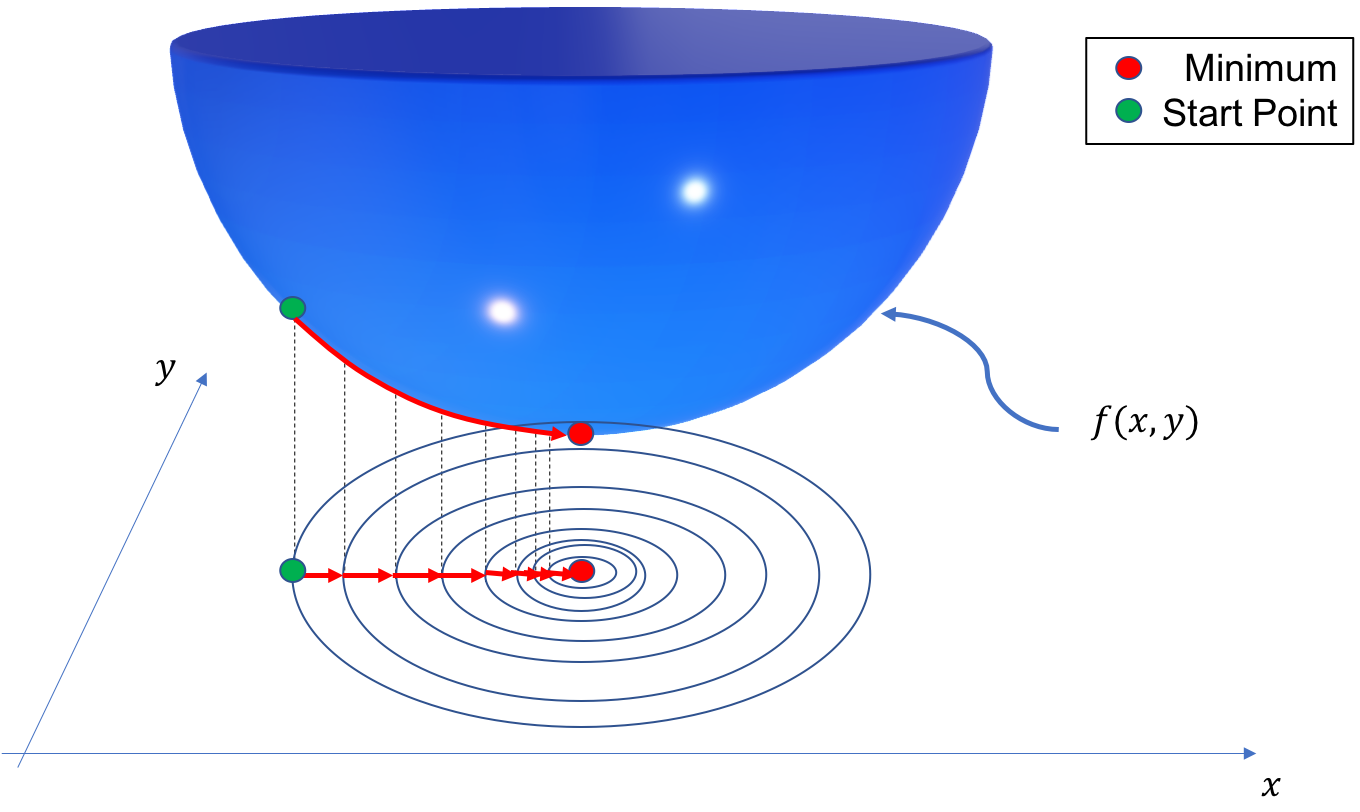
\includegraphics[width=1.0\linewidth]{fig-nlin/steepest_descent.png}}
  \caption{
  A very simple example of the gradient descent method. \label{fig:nlin:grad}
  }
\end{figure}
%\clearpage % flush figures fig:nlin:grad

Assume that we have a function $\mathbf{f}(\mathbf{x})$, that we would like to minimize. The gradient descent algorithm is simply to update parameters according to the derivative (gradient) of $\mathbf{f}$
\begin{equation}
\mathbf{x}_{k+1}=\mathbf{x}_{k}-\gamma\nabla\mathbf{f}.
\label{eq:nlin:stpdc}
\end{equation}
$\gamma$ is the learning rate, and a good choice of $\gamma$ is important. $\gamma$ might also change from one iteration to the other, and does not have to be constant.  

% --- begin exercise ---
\begin{doconceexercise}
\refstepcounter{doconceexercisecounter}

\exercisesection{Exercise \thedoconceexercisecounter: Gradient descent solution of linear regression}
                             

A very typical example is if we have a model and we would like to fit some parameters of the model to a data set (e.g.~linear regression). Assume that we have observations $(x_i,y_i)$ and model predictions $f(x_i,\mathbf{\beta})$, the model parameters are contained in the vector $\mathbf{\beta}$. The \emph{least square}, $S$, is the square of the sum of all the \emph{residuals}, i.e.~the difference between the observations and model predictions 
\begin{equation}
S=\sum_i(y_i-f(x_i,\mathbf{\beta}))^2.
\label{eq:nlin:lsq}
\end{equation}

Specializing to linear regression, we choose the model to be linear
\begin{equation}
f(x_i,\mathbf{\beta})=b_0+b_1x_i.
\label{eq:nlin:lin}
\end{equation}
Equation (\ref{eq:nlin:lsq}) now takes the form
\begin{equation}
S=\sum_i(y_i-b_0+b_1x_i)^2.
\label{eq:nlin:lsq2}
\end{equation}
The gradients are:
\begin{align}
\frac{\partial S}{\partial b_0}&=-2\sum_i(y_i-b_0+b_1x_i),\no\\ 
\frac{\partial S}{\partial b_1}&=-2\sum_i(y_i-b_0+b_1x_i)x_i,.
\label{eq:nlin:dlsq}
\end{align}

\begin{itemize}
\item Implement the gradient descent method using a constant learning rate of $10^{-3}$, to minimize the least square function

\item Test the linear regression on the data set $x_i=[0, 1, 2, 3, 4, 5, 6, 7, 8, 9]$, and $y=[1, 3, 2, 5, 7, 8, 8, 9, 10, 12]$, choose a starting value $(b_0,b_1)=(0,0)$. What happens if you increase the learning rate?
\end{itemize}

\noindent
% --- begin solution of exercise ---
\paragraph{Solution.}
Below is an implementation of the gradient descent method with a constant learning rate

























\begin{lstlisting}[language=python,style=blue1]
def gradient_descent(f,x,df, g=.001, prec=1e-8,MAXIT=10):
    '''Minimize f(x) by gradient descent.
    f   : min(f(x))
    x   : starting point 
    df  : derivative of f(x)
    g   : learning rate
    prec: desired precision
    
    Returns x when it is closer than eps to the root, 
    unless MAXIT are not exceeded
    '''
    x_old = x
    for n in range(MAXIT):
        plot_regression_line(x_old)  
        x_new = x_old - g*df(x_old)
        if(abs(np.max(x_new-x_old))<prec):
            print('Found solution:', x_new, 
                  ', after:', n, 'iterations.' )
            return x_new
        x_old=x_new
    print('Max number of iterations: ', MAXIT, ' reached.') 
    print('Try to increase MAXIT or decrease prec')
    print('Returning best guess, value of function is: ', f(x_new))
    return x_new

\end{lstlisting}


The linear regression is implemented as below



























































































































\begin{lstlisting}[language=python,style=blue1]
x_obs_ = np.array([0, 1, 2, 3, 4, 5, 6, 7, 8, 9]) 
y_obs_ = np.array([1, 3, 2, 5, 7, 8, 8, 9, 10, 12]) 
def plot_regression_line(b,x=x_obs_, y=y_obs_): 
    global N_
    # plotting the actual points as scatter plot 
    plt.scatter(x, y, color = "m", 
               marker = "o", s = 30,label="data") 
  
    # predicted response vector 
    y_pred = b[0] + b[1]*x
  
    # plotting the regression line
    if(len(b)>1):
#        plt.plot(x, y_pred, color = "g", label = "R-squared = {0:.3f}".format(b[2]))
        plt.plot(x, y_pred, color = "g", label = "iteration:" + str(N_) +", (b[0],b[1])= ({0:.3f}".format(b[0]) + ", {0:.3f})".format(b[1]))
        plt.legend()
    else:
        plt.plot(x, y_pred, color = "g")
  
    # putting labels 
    plt.xlabel('x') 
    plt.ylabel('y') 
    plt.grid()
    plt.legend()
#    plt.savefig('../fig-nlin/stdec'+str(N_)+'.png', bbox_inches='tight',transparent=True)
    N_=N_+1  
    # function to show plot 
    plt.show() 


def Jacobian(x,f,dx=1e-5):
    N=len(x)
    x0=np.copy(x)
    f0=f(x)
    J=np.zeros(shape=(N,N))
    for j in range(N):
        x[j] = x[j] +  dx
        for i in range(N):   
            J[i][j] = (f(x)[i]-f0[i])/dx
        x[j] = x[j] -  dx
    return J




def newton_rapson(x,f,J=None, jacobian=False, prec=1e-8,MAXIT=100):
    '''Approximate solution of f(x)=0 by Newtons method.
    The derivative of the function is calculated numerically
    f   : f(x)=0.
    J   : Jacobian
    x   : starting point  
    eps : desired precision
    
    Returns x when it is closer than eps to the root, 
    unless MAX_ITERATIONS are not exceeded
    '''
    MAX_ITERATIONS=MAXIT
    x_old = np.copy(x)
    for n in range(MAX_ITERATIONS):
        plot_regression_line(x_old) 
        if not jacobian:
            J_=Jacobian(x_old,f)
        else:
            J_=J(x_old)
        z=np.linalg.solve(J_,-f(x_old))
        x_new=x_old+z
        if(np.sum(abs(x_new-x_old))<prec):
            print('Found solution:', x_new, 
                  ', after:', n, 'iterations.' )
            return x_new
        x_old=np.copy(x_new)
    print('Max number of iterations: ', MAXIT, ' reached.') 
    print('Try to increase MAXIT or decrease prec')
    print('Returning best guess, value of function is: ', f(x_new))
    return x_new


def gradient_descent(f,x,df, g=.001, prec=1e-8,MAXIT=10):
    '''Minimize f(x) by gradient descent.
    f   : min(f(x))
    x   : starting point 
    df  : derivative of f(x)
    g   : learning rate
    prec: desired precision
    
    Returns x when it is closer than eps to the root, 
    unless MAXIT are not exceeded
    '''
    x_old = x
    for n in range(MAXIT):
        plot_regression_line(x_old)  
        x_new = x_old - g*df(x_old)
        if(abs(np.max(x_new-x_old))<prec):
            print('Found solution:', x_new, 
                  ', after:', n, 'iterations.' )
            return x_new
        x_old=x_new
    print('Max number of iterations: ', MAXIT, ' reached.') 
    print('Try to increase MAXIT or decrease prec')
    print('Returning best guess, value of function is: ', f(x_new))
    return x_new
#end

def S(b,x=x_obs_,y=y_obs_):
    return np.sum((y-b[0]-b[1]*x)**2)

def dS(b,x=x_obs_,y=y_obs_):
    return np.array([-2*np.sum(y-b[0]-b[1]*x),
                     -2*np.sum((y-b[0]-b[1]*x)*x)])

def J(b,x=x_obs_,y=y_obs_):
    N=len(b)
    J=np.zeros(shape=(N,N))
    xs=np.sum(x)
    J[0][0]=2*len(x)
    J[0][1]=2*xs
    J[1][0]=2*xs
    J[1][1]=2*np.sum(x*x)
    return J
N_=0
print('Gradient ')
b=np.array([0,0])

\end{lstlisting}

The first four iterations are shown in figure~\ref{fig:nlin:grsc}. If we choose a learning rate that is too high, we will move past the minimum, and the solution will oscillate. This can be avoided by lowering the learning rate as we iterate, by e.g.~replacing \texttt{g} with \texttt{g/(n+1)} in the implementation above.

\begin{figure}[!ht]  % fig:nlin:grsc
  \centerline{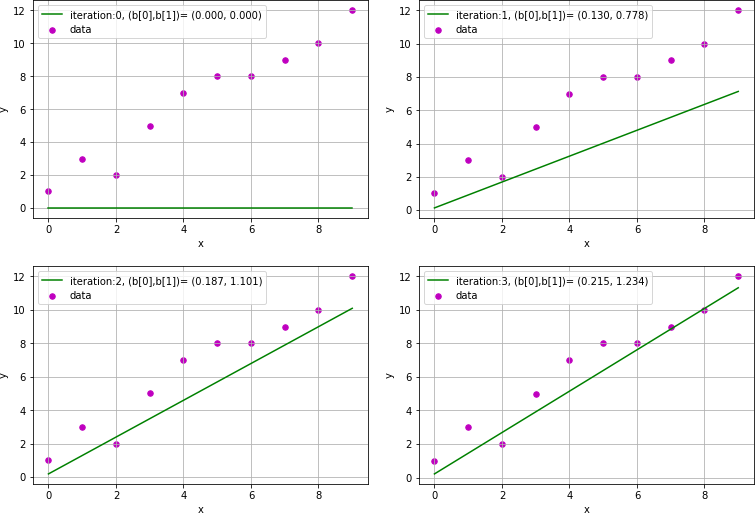
\includegraphics[width=1.0\linewidth]{fig-nlin/stdec_comb.png}}
  \caption{
  First four iterations of the gradient descent solution of linear regression. \label{fig:nlin:grsc}
  }
\end{figure}
%\clearpage % flush figures fig:nlin:grsc

% --- end solution of exercise ---

\end{doconceexercise}
% --- end exercise ---

\section{Other useful methods}

In this chapter we have covered the \emph{basic}, but you should now be well equipped to dive into other methods. We highly recommend \cite{press2001} as a starting point, although the code examples are written in C++, the theory is presented in a very accurate, but informal way.
\begin{itemize}
\item Brents method:  uses root bracketing, bisection, and inverse quadratic interpolation. The 1D method of choice if the function and not its derivative is known
\end{itemize}

\noindent
% !split

\chapter{Numerical integration}
\label{ch:numint}

\section{Algorithmic thinking}

The only way to improve in coding and algorithmic thinking is practice. The concept of one dimensional numerical integration is easy to understand, i.e.~to calculate the area under a curve. In this chapter we will implement several numerical methods, and it will serve as a very simple playground that illustrates the key aspects of numerical modeling

\begin{enumerate}
\item We start with a mathematical model (in this case an integral)

\item The mathematical model is formulated in discrete form 

\item Then we design an algorithm to solve the model 

\item The numerical solution for a test case is compared with the true solution (could be an analytical solution or data)

\item Error analysis: we investigate the accuracy of the algorithm by changing the number of iterations and/or make changes to the implementation or algorithm
\end{enumerate}

\noindent
The main point of this chapter is not to develop your own integration methods, the built in methods in Scipy will work in most cases. However, the way to break down the main task of calculating an integral into smaller tasks that is understandable by a computer, may work as a template for many different problems you would typically solve using a computer. A second motivation is that by analyzing the origin of numerical errors gives ideas for improving the algorithm, which is transferable to other problems.      

\subsection{The midpoint rule}
\index{midpoint method}
Numerical integration is encountered in numerous applications in physics and engineering sciences. 
Let us first consider the most simple case, a function $f(x)$, which is a function of one variable, $x$. The most straight forward way of calculating the area $\int_a^bf(x)dx$ is 
simply to divide the area under the function into $N$ equal rectangular slices with size $h=(b-a)/N$, as illustrated in figure~\ref{fig:numint:mid}. The area of one box is:
\begin{equation}
M(x_k,x_k+h)=f(x_k+\frac{h}{2}) h,\label{eq:numint:mid0}
\end{equation}
and the area of all the boxes is:
\begin{align}
I(a,b)&=\int_a^bf(x)dx\simeq\sum_{k=0}^{N-1}M(x_k,x_k+h)\nonumber\\ 
&=h\sum_{k=0}^{N-1}f(x_k+\frac{h}{2})=h\sum_{k=0}^{N-1}f(a+(k+\frac{1}{2})h).
\label{eq:numint:mid1}
\end{align}
Note that the sum goes from $k=0,1,\ldots,N-1$, a total of $N$ elements. We could have chosen to let the sum go from $k=1,2,\ldots,N$. 
In Python, C, C++ and many other programming languages the arrays start by indexing the elements from $0,1,\ldots$ to $N-1$, 
therefore we choose the convention of having the first element to start at $k=0$.

\begin{figure}[!ht]  % fig:numint:mid
  \centerline{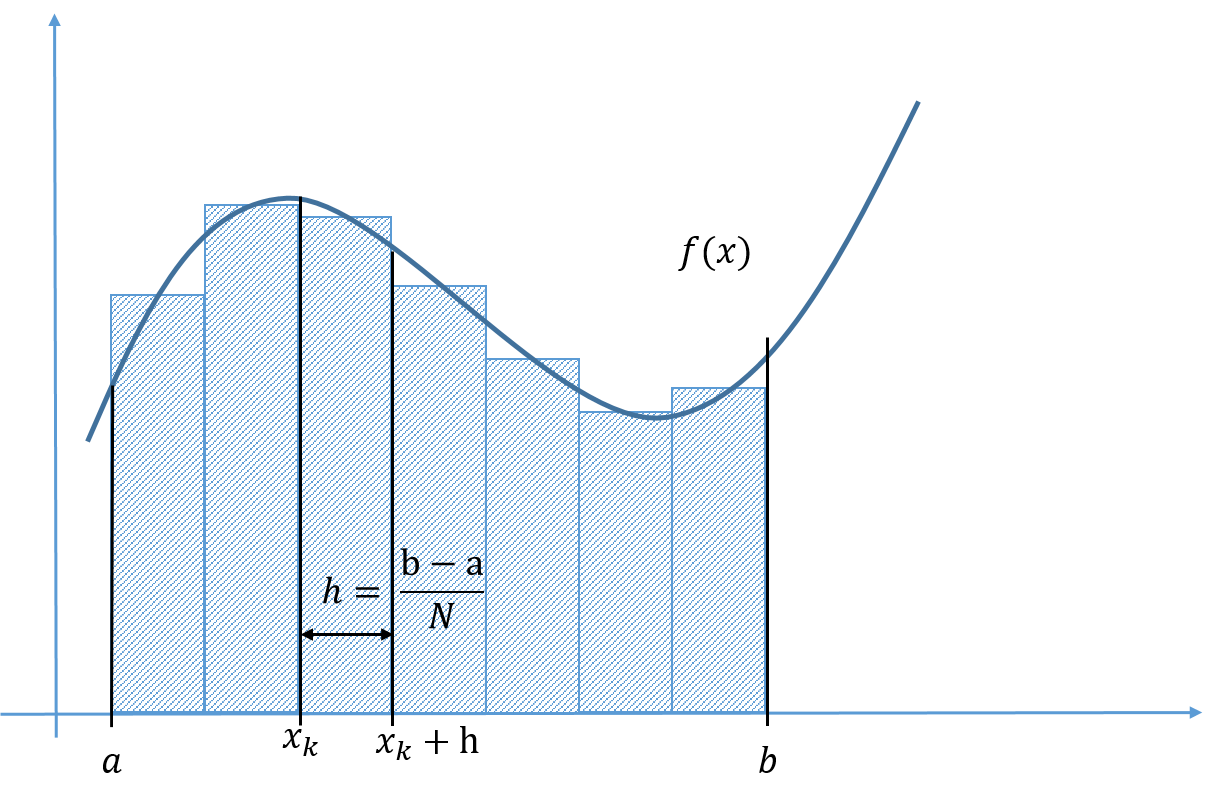
\includegraphics[width=0.9\linewidth]{fig-numint/func_sq.png}}
  \caption{
  Integrating a function with the midpoint rule. \label{fig:numint:mid}
  }
\end{figure}
%\clearpage % flush figures fig:numint:mid

Below is a Python code, where this algorithm is implemented for $\int_0^\pi\sin (x)dx$




















\begin{lstlisting}[language=python,style=blue1]
import numpy as np
# Function to be integrated
def f(x):
    return np.sin(x)

def midpoint(f,a,b,N):
    """
    f : function to be integrated on the domain [a,b]
    N : number of integration points
    """
    h=(b-a)/N
    x=np.arange(a+0.5*h,b,h)
    return h*np.sum(f(x))
N=10
a=0
b=np.pi
Area = midpoint(f,a,b,N)
print('Numerical value= ', Area)
print('Error= ', (2-Area)) # Analytical result is 2

\end{lstlisting}




\begin{graybox2admon}[Notice]
In the implementation above, we have taken advantage of Numpys ability to pass a vector to a function. This greatly enhances the speed and makes clean, readable code. If you were coding in a lower level programming language like Fortran, C or C++, you would probably implement the loop like (in Python syntax):





\begin{lstlisting}[language=python,style=blue1]
for k in range(0,N): # loop over k=0,1,..,N-1
    val = lower_limit+(k+0.5)*h # midpoint value
    area += func(val)
return area*h

\end{lstlisting}
\end{graybox2admon}




\subsection{The trapezoidal rule}
\index{trapezoidal method}
The numerical error in the above example is quite low, only about 2$\%$ for $N=5$. 
However, by just looking at the graph above it seems likely that we can develop a better algorithm by using trapezoids instead of rectangles, 
see figure~\ref{fig:numint:trap}.

\begin{figure}[!ht]  % fig:numint:trap
  \centerline{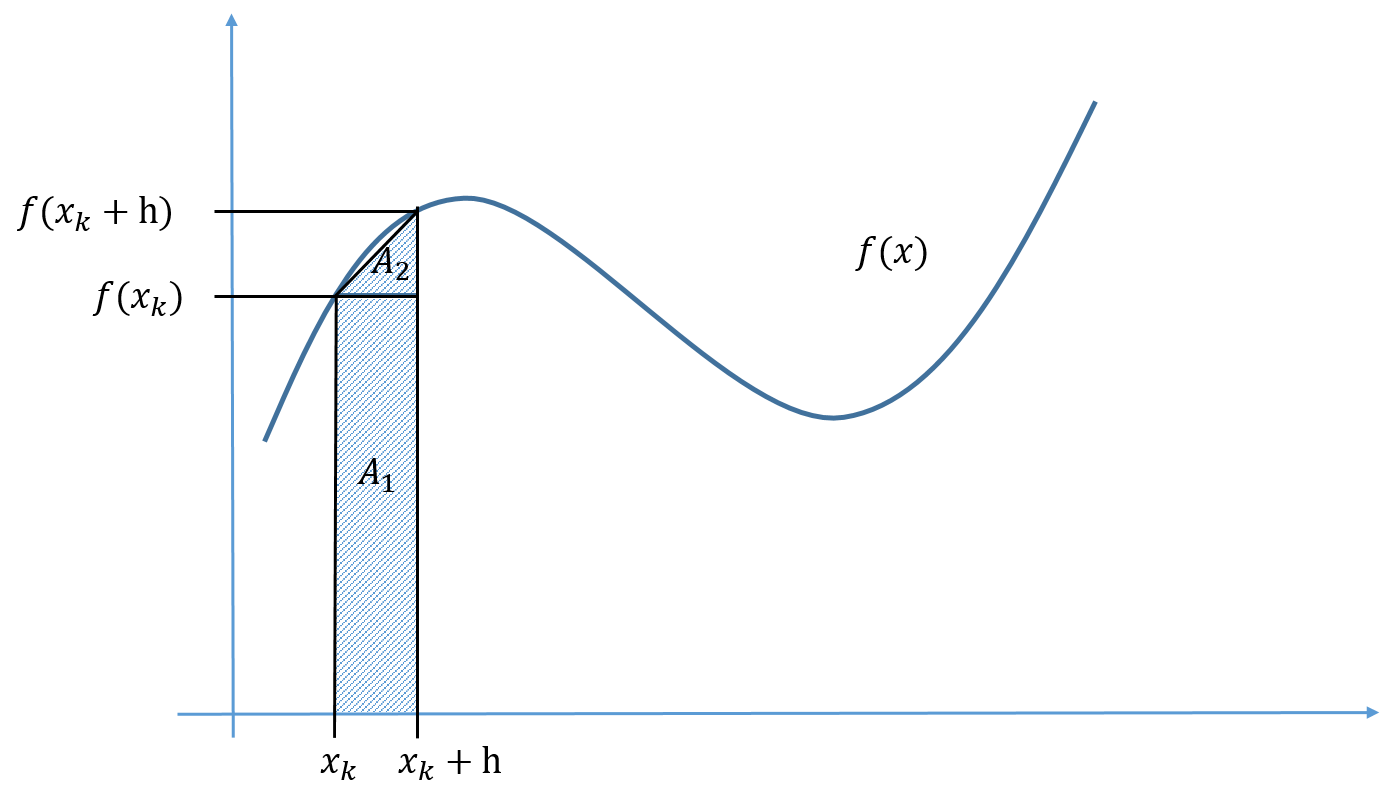
\includegraphics[width=0.9\linewidth]{fig-numint/func_tr.png}}
  \caption{
  Integrating a function with the trapezoidal rule. \label{fig:numint:trap}
  }
\end{figure}
%\clearpage % flush figures fig:numint:trap

Earlier we approximated the area using the midpoint value: $f(x_k+h/2)\cdot h$. Now we use $A=A_1+A_2$, where $A_1=f(x_k)\cdot h$ 
and $A_2=(f(x_k+h)-f(x_k))\cdot h/2$, hence the area of one trapezoid is:
\begin{equation}
A\equiv T(x_k,x_k+h)=(f(x_k+h)+f(x_k))h/2.
\end{equation}
This is the trapezoidal rule, and for the whole interval we get:
\begin{align}
I(a,b)&=\int_a^bf(x)dx\simeq\frac{1}{2}h\sum_{k=0}^{N-1}\left[f(x_k+h)+f(x_k)\right] \nonumber \\ 
&=h\left[\frac{1}{2}f(a)+f(a+h) + f(a+2h) +\nonumber\right. \\ 
&\left.\qquad\cdots + f(a+(N-2)h)+\frac{1}{2}f(b)\right]\nonumber \\ 
&=h\left[\frac{1}{2}f(a)+\frac{1}{2}f(b)+\sum_{k=1}^{N-2}f(a+k h)\right].
\end{align}
Note that this formula was bit more involved to derive, but it requires only one more function evaluations compared to the midpoint rule. 
Below is a python implementation:









\begin{lstlisting}[language=python,style=blue1]
def trapezoidal(f,a,b,N):
    """
    f : function to be integrated on the domain [a,b]
    N : number of integration points
    """
    h=(b-a)/N
    x=np.arange(a+h,b,h)
    return h*(0.5*f(a)+0.5*f(b)+np.sum(f(x)))

\end{lstlisting}


In the table below, we have calculated the numerical error for various values of $N$.



{\small   % for Springer style: small table font and more vspace

\vspace{4mm}

\begin{tabular}{cccc}
\hline
\multicolumn{1}{c}{ $N$ } & \multicolumn{1}{c}{ $h$ } & \multicolumn{1}{c}{ Error Midpoint } & \multicolumn{1}{c}{ Error Trapezoidal } \\
\hline
1   & 3.14  & -57\%          & 100\%             \\
5   & 0.628 & -1.66\%        & 3.31\%            \\
10  & 0.314 & -0.412\%       & 0.824\%           \\
100 & 0.031 & -4.11E-3\%     & 8.22E-3\%         \\
\hline
\end{tabular}

\vspace{4mm}

}


\noindent
Note that we get the surprising result that this algorithm performs poorer, a factor of 2 than the midpoint rule.
How can this be explained? By just looking at figure~\ref{fig:numint:mid}, we see that the midpoint rule actually over predicts the area from $[x_k,x_k+h/2]$ 
 and under predicts in the interval $[x_k+h/2,x_{k+1}]$ or vice versa. The net effect is that for many cases the midpoint rule give a slightly better 
 performance than the trapezoidal rule. In the next section we will investigate this more formally.

\subsection{Numerical errors on integrals}
\index{numerical integrals, error}
It is important to know the accuracy of the methods we are using, otherwise we do not know if the
computer produce correct results. In the previous examples we were able to estimate the error because we knew the analytical result. However, if we know the 
analytical result there is no reason to use the computer to calculate the result(!). Thus, we need a general method to estimate the error, and let the computer 
run until a desired accuracy is reached. 

In order to analyze the midpoint rule in more detail we approximate the function by a Taylor 
series at the midpoint between $x_k$ and $x_k+h$: 
\begin{align}
f(x)&=f(x_k+h/2)+f^\prime(x_k+h/2)(x-(x_k+h/2))\nonumber\\ 
&+\frac{1}{2!}f^{\prime\prime}(x_k+h/2)(x-(x_k+h/2))^2+\mathcal{O}(h^3)
\end{align}
Since $f(x_k+h/2)$ and its derivatives are constants it is straight forward to integrate $f(x)$:
\begin{align}
I(x_k,x_k+h)&=\int_{x_k}^{x_k+h}\left[f(x_k+h/2)+f^\prime(x_k+h/2)(x-(x_k+h/2))\right.\nonumber\\ 
&\left.+\frac{1}{2!}f^{\prime\prime}(x_k+h/2)(x-(x_k+h/2))^2+\mathcal{O}(h^3)\right]dx
\end{align}
The first term is simply the midpoint rule, to evaluate the two other terms we make the substitution: $u=x-x_k$:
\begin{align}
I(x_k,x_k+h)&=f(x_k+h/2)\cdot h+f^\prime(x_k+h/2)\int_0^h(u-h/2)du\nonumber\\ 
&+\frac{1}{2}f^{\prime\prime}(x_k+h/2)\int_0^h(u-h/2)^2du+\mathcal{O}(h^4)\nonumber\\ 
&=f(x_k+h/2)\cdot h-\frac{h^3}{24}f^{\prime\prime}(x_k+h/2)+\mathcal{O}(h^4).
\end{align}
Note that all the odd terms cancels out, i.e $\int_0^h(u-h/2)^m=0$ for $m=1,3,5\ldots$. Thus the error for the midpoint rule, $E_{M,k}$, on this particular interval is:
\begin{equation}
E_{M,k}=I(x_k,x_k+h)-f(x_k+h/2)\cdot h=-\frac{h^3}{24}f^{\prime\prime}(x_k+h/2),
\end{equation}
where we have ignored higher order terms. We can easily sum up the error on all the intervals, but clearly $f^{\prime\prime}(x_k+h/2)$ will 
not, in general, have the same value on all intervals. However, an upper bound for the error can be found by replacing $f^{\prime\prime}(x_k+h/2)$ 
with the maximal value on the interval $[a,b]$, $f^{\prime\prime}(\eta)$:
\begin{align}
E_{M}&=\sum_{k=0}^{N-1}E_{M,k}=-\frac{h^3}{24}\sum_{k=0}^{N-1}f^{\prime\prime}(x_k+h/2)\leq-\frac{Nh^3}{24}f^{\prime\prime}(\eta),\label{eq:numint:em}\\ 
E_{M}&\leq-\frac{(b-a)^3}{24N^2}f^{\prime\prime}(\eta),
\end{align}
where we have used $h=(b-a)/N$. We can do the exact same analysis for the trapezoidal rule, but then we expand the function around $x_k-h$ instead of the midpoint. 
The error term is then:
\begin{equation}
E_T=\frac{(b-a)^3}{12N^2}f^{\prime\prime}(\overline{\eta}).
\end{equation}
At the first glance it might look like the midpoint rule always is better than the trapezoidal rule, but note that the second derivative is 
evaluated in different points ($\eta$ and $\overline{\eta}$). Thus it is possible to construct examples where the midpoint rule performs poorer 
than the trapezoidal rule.

Before we end this section we will rewrite the error terms in a more useful form as it is not so easy to evaluate 
$f^{\prime\prime}(\eta)$ (since we do not know which value of $\eta$ to use). By taking a closer look at equation (\ref{eq:numint:em}), 
we see that it is closely related to the midpoint rule for $\int_a^bf^{\prime\prime}(x)dx$, hence:
\begin{align}
E_{M}&=-\frac{h^2}{24}h
\sum_{k=0}^{N-1}f^{\prime\prime}(x_k+h/2)\simeq-\frac{h^2}{24}\int_a^b
f^{\prime\prime}(x)dx\\ 
E_M&\simeq\frac{h^2}{24}\left[f^\prime(b)-f^\prime(a)\right]=-\frac{(b-a)^2}{24N^2}\left[f^\prime(b)-f^\prime(a)\right]
\end{align}
The corresponding formula for the trapezoid formula is:
\begin{equation}
E_T\simeq \frac{h^2}{12}\left[f^\prime(b)-f^\prime(a)\right]=\frac{(b-a)^2}{12N^2}\left[f^\prime(b)-f^\prime(a)\right]
\end{equation}
\subsection{Practical estimation of errors on integrals (Richardson extrapolation)}
\index{Richardson extrapolation}
\label{sec:numint:parct}
From the example above we were able to estimate the number of steps needed to reach (at least) a certain precision. 
In many practical cases we do not deal with functions, but with data and it can be difficult to evaluate the derivative. 
We also saw from the example above that the algorithm gives a higher precision than what we asked for. 
How can we avoid doing too many iterations? A very simple solution to this question is to double the number of intervals until 
a desired accuracy is reached. The following analysis holds for both the trapezoid and midpoint method, because in both cases 
the (global) error scale as $h^2$\footnote{You can do the following analysis by assuming that the local error is $h^3$, but then you need to take into account that you need to take twice as many steps, which will give the same result.}.

Assume that we have evaluated the integral with a step size $h_1$, and the computed result is $I_1$. 
Then we know that the true integral is $I=I_1+c h_1^2$, where $c$ is a constant that is unknown. If we now half the step size: $h_2=h_1/2$, 
then we get a new (better) estimate of the integral, $I_2$, which is related to the true integral $I$ as: $I=I_2+c h_2^2$. 
Taking the difference between $I_2$ and $I_1$ give us an estimation of the error:
\begin{equation}
I_2-I_1=I-c h_2^2-(I-ch_1^2)=3c h_2^2,
\end{equation}
where we have used the fact that $h_1=2h_2$, Thus the error term is:
\begin{equation}
E(a,b)=c h_2^2=\frac{1}{3}(I_2-I_1).
\end{equation}
This might seem like we need to evaluate the integral twice as many times as needed. This is not the case, by choosing to exactly 
half the spacing we only need to evaluate for the values that lies halfway between the original points. We will demonstrate how 
to do this by using the trapezoidal rule, because it operates directly on the $x_k$ values and not the midpoint values. 
The trapezoidal rule can now be written as:
\begin{align}
I_2(a,b)&=h_2\left[\frac{1}{2}f(a)+\frac{1}{2}f(b)+\sum_{k=1}^{N_2-1}f(a+k h_2)\right],\\ 
&=h_2\left[\frac{1}{2}f(a)+\frac{1}{2}f(b)+\sum_{k=\text{even values}}^{N_2-1}f(a+k h_2)\right.\nonumber\\ 
&\left.\qquad+\sum_{k=\text{odd values}}^{N_2-1}f(a+k h_2)\right],
\end{align}
in the last equation we have split the sum into odd an even values. The sum over the even values can be rewritten:
\begin{equation}
\sum_{k=\text{even values}}^{N_2-1}f(a+k h_2)=\sum_{k=0}^{N_1-1}f(a+2k h_2)=\sum_{k=0}^{N_1-1}f(a+k h_1),
\end{equation}
note that $N_2$ is replaced with $N_1=N_2/2$, we can now rewrite $I_2$ as:
\begin{align}
I_2(a,b)&=h_2\left[\frac{1}{2}f(a)+\frac{1}{2}f(b)+\sum_{k=0}^{N_1-1}f(a+k h_1)\right.\nonumber\\ 
&\left.+\sum_{k=\text{odd values}}^{N_2-1}f(a+k h_2)\right]
\end{align}
Note that the first terms are actually the trapezoidal rule for $I_1$, hence:
\begin{equation}
I_2(a,b)=\frac{1}{2}I_1(a,b)+h_2\sum_{k=\text{odd values}}^{N_2-1}f(a+k h_2).
\end{equation}
The factor $1/2$ in front of $I_1(a,b)$, appears because $h_2=h_1/2$. 
A possible algorithm is then:
\begin{enumerate}
\item Choose a low number of steps to evaluate the integral, $I_0$, the first time, e.g.~$N_0=1$

\item Double the number of steps, $N_1=2N_0$ 

\item Calculate the missing values by summing over the odd number of steps $\sum_{k=\text{odd values}}^{N_1-1}f(a+k h_1)$

\item Check if $E_1(a,b)=\frac{1}{3}(I_1-I_0)$ is lower than a specific tolerance

\item If yes quit, if not, return to 2, and continue until $E_i(a,b)=\frac{1}{3}(I_{i+1}-I_{i})$ is lower than the tolerance  
\end{enumerate}

\noindent
Below is a Python implementation:
























\begin{lstlisting}[language=python,style=blue1]
def int_adaptive_trapez2(lower_limit, upper_limit,func,tol):
    """
    adaptive quadrature, integrate a function from lower_limit
    to upper_limit within tol*(upper_limit-lower_limit)

    """
    S=[]
    S.append([lower_limit,upper_limit])
    I=0
    iterations=0
    while S:
        iterations +=1
        a,b=S.pop(-1) # last element
        m=(b+a)*0.5   # midpoint
        I1=0.5*(b-a)*(func(a)+func(b)) #trapezoidal for 1 interval 
        I2=0.25*(b-a)*(func(a)+func(b)+2*func(m)) #trapezoidal for 2 intervals
        if(np.abs(I1-I2)<3*np.abs((b-a)*tol)):
            I+=I2     # accuarcy met
        else:
            S.append([a,m]) # half the interval 
            S.append([m,b])
    print("Number of iterations: ", iterations)
    return I

\end{lstlisting}


If you compare the number of terms used in the adaptive trapezoidal rule, which was developed by halving the step size, and the adaptive midpoint rule that was derived on the basis of the theoretical error term, you will find the adaptive midpoint rule is more efficient. So why go through all this trouble? In the next section we will see that the development we did for the adaptive trapezoidal rule is closely related to Romberg integration, which is \emph{much} more effective.

\section{Romberg integration}
\index{Romberg integration}
The adaptive algorithm for the trapezoidal rule in the previous section can be easily improved by remembering 
that the true integral was given by\footnote{Note that all odd powers of $h$ is equal to zero, thus the corrections are always in even powers.} : $I=I_i+ch_i^2+\mathcal{O}(h^4)$. The error term was in the previous example only used to 
check if the desired tolerance was achieved, but we could also have added it to our estimate of the integral to reach an accuracy to fourth order:

\begin{equation}
I=I_{i+1}+ch^2+\mathcal{O}(h^4)=I_{i+1}+\frac{1}{3}\left[I_{i+1}-I_{i}\right]+\mathcal{O}(h^4).
\end{equation}
As before the error term $\mathcal{O}(h^4)$, can be written as: $ch^4$. Now we can proceed as in the previous section: First we estimate the 
integral by one step size $I_i=I+ch_i^4$, next we half the step size $I_{i+1}=I+ch_{i+1}^4$ and use these two estimates to calculate the error term:
\begin{align}
I_{i+1}-I_{i}&=I-c h_{i+1}^4-(I-ch_i^4)=-c h_{i+1}^4+c(2h_{i+1})^4=15c h_{i+1}^4,\nonumber\\ 
ch_{i+1}^4&=\frac{1}{15}\left[I_{i+1}-I_{i}\right]+\mathcal{O}(h^6).
\end{align}
but now we are in the exact situation as before, we have not only the error term but the correction up to order $h^4$ for this integral:
\begin{equation}
I=I_{i+1}+\frac{1}{15}\left[I_{i+1}-I_{i}\right]+\mathcal{O}(h^6).\label{eq:numint:rom}
\end{equation}
Each time we half the step size we also gain a higher order accuracy in our numerical algorithm. Thus, there are two iterations going on at the same time; 
one is the iteration that half the step size ($i$), and the other one is the increasing number of higher order terms added (which we will denote $m$). 
We need to improve our notation, and replace the approximation of the integral ($I_i$) with $R_{i,m}$. Equation (\ref{eq:numint:rom}), can now 
be written:
\begin{equation}
I=R_{i+1,2}+\frac{1}{15}\left[R_{i+1,2}-R_{i,2}\right]+\mathcal{O}(h^6).
\end{equation}
A general formula valid for any $m$ can be found by realizing:
\begin{align}
I&=R_{i+1,m+1}+c_mh_i^{2m+2}+\mathcal{O}(h_i^{2m+4})\label{eq:numint:rom0}\\ 
I&=R_{i,m+1}+c_mh_{i-1}^{2m+2}+\mathcal{O}(h_{i-1}^{2m+4})\nonumber\\ 
&=R_{i,m+1}+2^{2m+2}c_mh_{i}^{2m+2}+\mathcal{O}(h_{i-1}^{2m+4}),\label{eq:numint:rom1}
\end{align}
where, as before $h_{i-1}=2h_i$. Subtracting equation (\ref{eq:numint:rom0}) and (\ref{eq:numint:rom1}), we find an expression for the error term:
\begin{align}
c_mh_{i}^{2m+2}&=\frac{1}{4^{m+1}-1}(R_{i,m}-R_{i-1,m})\label{eq:numint:rom2}
\end{align}
Then the estimate for the integral in equation (\ref{eq:numint:rom1}) is:
\begin{align}
I&=R_{i,m+1}+\mathcal{O}(h_i^{2m+2})\\ 
R_{i,m+1}&=R_{i,m}+\frac{1}{4^{m+1}-1}(R_{i+1,m}-R_{i,m}).
\end{align}
A possible algorithm is then:

\begin{enumerate}
\item Evaluate $R_{0,0}=\frac{1}{2}\left[f(a)+f(b)\right](b-a)$ as the first estimate

\item Double the number of steps, $N_{i+1}=2N_i$ or half the step size $h_{i+1}=h_i/2$ 

\item Calculate the missing values by summing over the odd number of steps $\sum_{k=\text{odd values}}^{N_1-1}f(a+k h_{i+1})$

\item Correct the estimate by adding \emph{all} the higher order error term $R_{i,m+1}=R_{i,m}+\frac{1}{4^m-1}(R_{i+1,m+1}-R_{i,m+1})$

\item Check if the error term is lower than a specific tolerance $E_{i,m}(a,b)=\frac{1}{4^{m+1}-1}(R_{i,m}-R_{i-1,m})$, if yes quit, if no goto 2, increase $i$ and $m$ by one
\end{enumerate}

\noindent
The algorithm is illustrated in figure~\ref{fig:numint:romberg}.

\begin{figure}[!ht]  % fig:numint:romberg
  \centerline{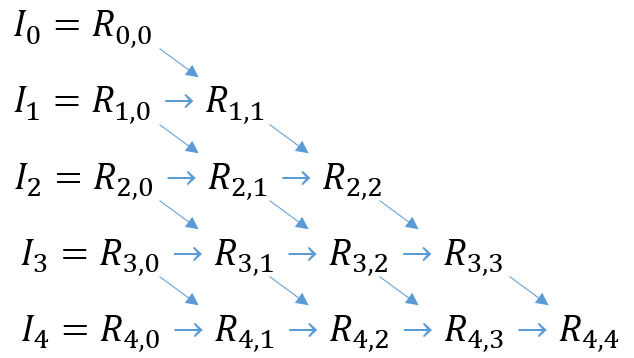
\includegraphics[width=0.5\linewidth]{fig-numint/romberg.png}}
  \caption{
  Illustration of the Romberg algorithm. Note that for each new evaluation of the integral $R_{i,0}$, all the correction terms $R_{i,m}$ (for $m>0$) must be evaluated again. \label{fig:numint:romberg}
  }
\end{figure}
%\clearpage % flush figures fig:numint:romberg

Note that the tolerance term is not the correct one as it uses the error estimate for the current step, 
which we also use correct the integral in the current step to reach a higher accuracy. 
Thus the error on the integral will always be lower than the user specified tolerance.
Below is a Python implementation:










































\begin{lstlisting}[language=python,style=blue1]
def int_romberg(func,a, b,tol,show=False):
    """ calculates the area of func on the domain [a,b]
        for the given tol, if show=True the triangular
        array of intermediate results are printed """
    Nmax = 100
    R = np.empty([Nmax,Nmax]) # storage buffer
    h = (b-a) # step size
    R[0,0]    =.5*(func(a)+func(b))*h
    N = 1
    for i in range(1,Nmax):
        h /= 2
        N *= 2
        odd_terms=0
        for k in range (1,N,2): # 1, 3, 5, ... , N-1
            val        = a + k*h
            odd_terms += func(val)
		# add the odd terms to the previous estimate	
        R[i,0]   = 0.5*R[i-1,0] + h*odd_terms 
        for m in range(i): 
			# add all higher order terms in h
            R[i,m+1]   = R[i,m] + (R[i,m]-R[i-1,m])/(4**(m+1)-1)                  
		# check tolerance, best guess			
        calc_tol = abs(R[i,i]-R[i-1,i-1])       
        if(calc_tol<tol):
            break  # estimated precision reached 
    if(i == Nmax-1):
        print('Romberg routine did not converge after ',
              Nmax, 'iterations!')
    else:      
        print('Number of intervals = ', N)

    if(show==True):
        elem = [2**idx for idx in range(i+1)]
        print("Steps StepSize Results")
        for idx in range(i+1):
            print(elem[idx],' ',
                  "{:.6f}".format((b-a)/2**idx),end = ' ')
            for l in range(idx+1):
                print("{:.6f}".format(R[idx,l]),end = ' ')
            print('')  
    return R[i,i] #return the best estimate

\end{lstlisting}


Note that the Romberg integration only uses 32 function evaluations to reach a precision of $10^{-8}$, whereas the adaptive midpoint and trapezoidal rule in the previous
section uses 20480 and 9069 function evaluations, respectively. 

\subsection{Alternative implementation of adaptive integration}
Before we proceed, we will consider an alternative implementation of the adaptive method presented in the previous sections, with the following modification
\begin{enumerate}
\item We will use Simpsons rule (see the exercise at the end), which takes the following form $\int_a^bf(x)dx\simeq\frac{h}{6}\left[f(a)+4f(a+\frac{h}{2})+2f(a+h)+ 4f(a+3\frac{h}{2})+2f(a+2h)+\cdots+f(b)\right]$

\item We only divide the intervals needed to reach the desired accuracy.
\end{enumerate}

\noindent
Simpsons rule is accurate up to $\mathcal{O}(h^4)$, and by following the same arguments as above we can estimate the error as $E_i(a,b)=\frac{1}{15}(I_{i+1}-I_{i})$. The factor 1/15 (as opposed to 1/3) originates from the higher order accuracy. The integration proceeds as follows
\begin{itemize}
\item \texttt{S} is an empty list

\item \texttt{S.append([a,b])}

\item $I=0$

\item \texttt{while S not empty do:}
\begin{itemize}

  \item \texttt{[a,b]=S.pop(-1)}

  \item $m=(b+a)/2$

  \item $I_1=$ \Verb!simpson_step(a,b)!

  \item $I_2=$ \Verb!simpson_step(a,m)+simpson_step(m,b)!

  \item if $|I_1-I_2|<15|b-a|\cdot tol$
\begin{itemize}

    \item $I+=I_2$

\end{itemize}

\noindent
  \item else:
\begin{itemize}

    \item \texttt{S.append([a,m])}

    \item \texttt{S.append([m,b])}

\end{itemize}

\noindent
  \item return $I$
\end{itemize}

\noindent
\end{itemize}

\noindent
Note the use of the list \texttt{S}, we remove the interval $[a,b]$ from the list and calculates the integral. If the integral is not accurate enough we add to new intervals to the list, and continue until we reach the desired accuracy, then we proceed with the next interval. Since we remove (\texttt{pop}) the element from the list, we know that we will finish the evaluation once the list is empty. This algorithm allows for different sub interval to have different degrees of subdivisions, contrary to Rombergs algorithm. The full python implementation is shown below



























\begin{lstlisting}[language=python,style=blue1]
def simpson_step(a, b,func):
    m=0.5*(a+b)
    return (b-a)/6*(func(a)+func(b)+4*func(m))

def int_adaptive_simpson(func,a, b,tol):
    """
    adaptive quadrature, integrate a function from a
    to b within tol*(b-a) uses simpsons rule
    """
    S=[]
    S.append([a,b])
    I=0
    iterations=0
    while S:
        iterations +=1
        a,b=S.pop(-1) # last element
        m=(b+a)*0.5   # midpoint
        I1=simpson_step(a,b,func) #simpsons for 1 interval 
        I2=simpson_step(a,m,func)+simpson_step(m,b,func) # ...2 intervals
        if(np.abs(I1-I2)<15*np.abs((b-a)*tol)):
            I+=I2     # accuarcy met
        else:
            S.append([a,m]) # half the interval 
            S.append([m,b])
    print("Number of iterations: ", iterations)
    return I

\end{lstlisting}


\section{Gaussian quadrature}
\index{Gaussian quadrature}
Many of the methods we have looked into are of the type:
\begin{align}
	\int_a^b f(x) dx = \sum_{k=0}^{N-1} \omega_k f(x_k),\label{eq:numint:qq1}
\end{align}
where the function is evaluated at fixed interval. For the midpoint rule $\omega_k=h$ for all values of $k$, for the trapezoid rule 
$\omega_k=h/2$ for the endpoints and $h$ for all the interior points. 
For the Simpsons rule (see exercise) $\omega_k=h/3, 4h/3,2h/3,4h/3,\ldots,4h/3,h/3$. 
Note that all the methods we have looked at so far samples the function in equal spaced points, $f(a+k h)$, 
for $k=0, 1, 2\ldots, N-1$. If we now allow for the function to be evaluated at unevenly spaced points, we can do a lot better. 
This realization is the basis for Gaussian Quadrature. We will explore this in the following, 
but to make the development easier and less cumbersome, we transform the integral from the domain $[a,b]$ to $[-1,1]$:
\begin{align}
\int_a^bf(t)dt&=\frac{b-a}{2}\int_{-1}^{1}f(x)dx\text{ , where:}\\ 
x&=\frac{2}{b-a}t-\frac{b+a}{b-a}.
\end{align}
The factor in front comes from the fact that $dt=(b-a)dx/2$, thus we can develop our algorithms on the domain $[-1,1]$, 
and then do the transformation back using: $t=(b-a)x/2+(b+a)/2$.



\begin{graybox2admon}[Notice]
The idea we will explore is as follows:
If we can approximate the function to be integrated on the domain $[-1,1]$ (or on $[a,b]$) as a 
polynomial of as \emph{large a degree as possible}, then the numerical integral of this polynomial will be very close to the integral of the 
function we are seeking.
\end{graybox2admon}



This idea is best understood by a couple of examples. Assume that we want to use $N=1$ in equation (\ref{eq:numint:qq1}):
\begin{equation}
\int_{-1}^{1}f(x)\,dx\simeq\omega_0f(x_0).
\end{equation}
We now choose $f(x)$ to be a polynomial of as large a degree as possible, but with the requirement that the integral is exact. If $f(x)=1$, we get:
\begin{equation}
\int_{-1}^{1}f(x)\,dx=\int_{-1}^{1}1\,dx=2=\omega_0,
\end{equation}
hence $\omega_0=2$. If we choose $f(x)=x$, we get:
\begin{equation}
\int_{-1}^{1}f(x)\,dx=\int_{-1}^{1}x\,dx=0=\omega_0f(x_0)=2x_0,
\end{equation}
hence $x_0=0$. 


\begin{graybox2admon}[The Gaussian integration rule for $N=1$ is:]

\begin{align}
&\int_{-1}^{1}f(x)\,dx\simeq 2f(0)\text{, or: }\nonumber\\ 
&\int_{a}^{b}f(t)\,dt\simeq\frac{b-a}{2}\,2f(\frac{b+a}{2})=(b-a)f(\frac{b+a}{2}).
\end{align}
\end{graybox2admon}




This equation is equal to the midpoint rule, by choosing $b=a+h$ we reproduce equation (\ref{eq:numint:mid0}). If we choose $N=2$:
\begin{equation}
\int_{-1}^{1}f(x)\,dx\simeq\omega_0f(x_0)+\omega_1f(x_1),
\end{equation}
we can show that now $ f(x)=1,\,x,\,x^2\,x^3$ can be integrated exact:
\begin{align}
\int_{-1}^{1}1\,dx&=2=\omega_0f(x_0)+\omega_1f(x_1)=\omega_0+\omega_1\,,\\ 
\int_{-1}^{1}x\,dx&=0=\omega_0f(x_0)+\omega_1f(x_1)=\omega_0x_0+\omega_1x_1\,,\\ 
\int_{-1}^{1}x^2\,dx&=\frac{2}{3}=\omega_0f(x_0)+\omega_1f(x_1)=\omega_0x_0^2+\omega_1x_1^2\,,\\ 
\int_{-1}^{1}x^3\,dx&=0=\omega_0f(x_0)+\omega_1f(x_1)=\omega_0x_0^3+\omega_1x_1^3\,,
\end{align}
hence there are four unknowns and four equations. The solution is: $\omega_0=\omega_1=1$ and $x_0=-x_1=1/\sqrt{3}$.



\begin{graybox2admon}[The Gaussian integration rule for $N=2$ is:]
\begin{align}
\int_{-1}^{1}f(x)\,dx&\simeq f(-\frac{1}{\sqrt{3}})+f(\frac{1}{\sqrt{3}})\, \text{, or:}\\ 
\int_{a}^{b}f(x)\,dx&\simeq \frac{b-a}{2}\left[f(-\frac{b-a}{2}\frac{1}{\sqrt{3}}+\frac{b+a}{2})
+f(\frac{b-a}{2}\frac{1}{\sqrt{3}}+\frac{b+a}{2})\right].
\end{align}
\end{graybox2admon}












\begin{lstlisting}[language=python,style=blue1]
def int_gaussquad2(func, lower_limit, upper_limit):
    x   = np.array([-1/np.sqrt(3.),1/np.sqrt(3)])
    w   = np.array([1, 1])
    xp  = 0.5*(upper_limit-lower_limit)*x
    xp += 0.5*(upper_limit+lower_limit)
    area = np.sum(w*func(xp))
    return area*0.5*(upper_limit-lower_limit)

\end{lstlisting}


\paragraph{The case N=3.}
For the case $N=3$, we find that $f(x)=1,x,x^2,x^3,x^4,x^5$ can be integrated exactly:
\begin{align}
\int_{-1}^{1}1\,dx&=2=\omega_0+\omega_1+\omega_2\,,\\ 
\int_{-1}^{1}x\,dx&=0=\omega_0x_0+\omega_1x_1+\omega_2x_2\,,\\ 
\int_{-1}^{1}x^2\,dx&=\frac{2}{3}=\omega_0x_0^2+\omega_1x_1^2+\omega_2x_2^2\,,\\ 
\int_{-1}^{1}x^3\,dx&=0=\omega_0x_0^3+\omega_1x_1^3+\omega_2x_2^3\,,\\ 
\int_{-1}^{1}x^4\,dx&=\frac{2}{5}=\omega_0x_0^4+\omega_1x_1^4+\omega_2x_2^4\,,\\ 
\int_{-1}^{1}x^5\,dx&=0=\omega_0x_0^5+\omega_1x_1^5+\omega_2x_2^5\,,
\end{align}
the solution to these equations are $\omega_{0,1,2}=5/9, 8/9, 5/9$ and $x_{1,2,3}=-\sqrt{3/5},0,\sqrt{3/5}$. Below is a Python implementation:








\begin{lstlisting}[language=python,style=blue1]
def int_gaussquad3(lower_limit, upper_limit,func):
    x  = np.array([-np.sqrt(3./5.),0.,np.sqrt(3./5.)])
    w  = np.array([5./9., 8./9., 5./9.])
    xp = 0.5*(upper_limit-lower_limit)*x
    xp += 0.5*(upper_limit+lower_limit)
    area = np.sum(w*func(xp))
    return area*0.5*(upper_limit-lower_limit)

\end{lstlisting}


Note that the Gaussian quadrature converges very fast. From $N=2$ to $N=3$ function evaluation we reduce the error (in this specific case) 
from 6.5\% to 0.1\%. Our standard trapezoidal formula needs more than 20 function evaluations to achieve this, the Romberg method uses 4-5 function
evaluations. How can this be? If we use the standard Taylor formula for the function to be integrated, we know that for $N=2$ the Taylor 
formula must be integrated up to $x^3$, so the error term is proportional to $h^4f^{(4)}(\xi)$ (where $\xi$ is some x-value in $[a,b]$). 
$h$ is the step size, and we can replace it with $h\sim (b-a)/N$, thus the error scale as $c_N/N^4$ (where $c_N$ is a constant). 
Following the same argument, we find for $N=3$ that the error term is $h^6f^{(6)}(\xi)$ or that the error term scale as $c_N/N^6$. 
Each time we increase $N$ by a factor of one, the error term reduces by $N^2$. Thus if we evaluate the integral for $N=10$, 
increasing to $N=11$ will reduce the error by a factor of $11^2=121$.

\subsection{Error term on Gaussian integration}
\index{Gaussian quadrature, error term}
The Gaussian integration rule of order $N$ integrates exactly a polynomial of order $2N-1$. 
From Taylors error formula, see equation (\ref{eq:taylor:error}) in Chapter~\ref{ch:taylor},
we can easily see that the error term must be of order $2N$, and be proportional to $f^{(2N)}(\eta)$, see \cite{stoer2013} for more details on the derivation of error terms. The drawback with an analytical error term derived from series expansion is that it involves the derivative of the function. As we have already explained, this is very unpractical and it is much more practical to use the methods described in section~\ref{sec:numint:parct}. Let us consider this in more detail, assume that we evaluate the integral using first a Gaussian integration rule with $N$ points, and then $N+1$ points. Our estimates of the "exact" integral, $I$,  would then be:
\begin{align}
 I&=I_N+ch_{N}^{2N},\label{eq:numint:gerr1}\\ 
 I&=I_{N+1}+ch_{N+1}^{2N+1}.
\label{eq:numint:gerr2}
\end{align}
In principle $h_{N+1}\neq h_{N}$, but in the following we will assume that $h_N\simeq h_{N+1}$, and $h\ll 1$. Subtracting equation (\ref{eq:numint:gerr1}) and (\ref{eq:numint:gerr2}) we can show that a reasonable estimate for the error term $ch^{2N}$ would be:
\begin{equation}
ch^N= I_{N+1}-I_N.
\end{equation}
If this estimate is lower than a given tolerance we can be quite confident that the higher order estimate $I_{N+1}$ approximate the true integral within our error estimate. This is the method implemented in SciPy, \href{{https://docs.scipy.org/doc/scipy-0.14.0/reference/generated/scipy.integrate.quadrature.html}}{\nolinkurl{integrate.quadrature}\footnote{\texttt{https://docs.scipy.org/doc/scipy-0.14.0/reference/generated/scipy.integrate.quadrature.html}}}

\subsection{Common weight functions for classical Gaussian quadratures}
\section{Integrating functions over an infinite range}
\index{numerical integral, infinite}
Integrating a function over an infinite range can be done by the following trick. Assume that we would like to evaluate
\begin{equation}
\int_a^\infty f(x) dx.
\label{eq:numint:inf}
\end{equation}
If we introduce the following substitution
\begin{equation}
z=\frac{x-a}{1+x-a},
\label{eq:numint:infs}
\end{equation}
or equivalently
\begin{equation}
x=a+\frac{z}{1-z},
\label{eq:numint:infs2}
\end{equation}
then if $x=a$, $z=0$, and if $x\to\infty$ then $z\to1$, hence:
\begin{equation}
\int_a^\infty f(x) dx = \int_0^1 f(a+\frac{z}{1-z}) \frac{dz}{(1-z)^2}.
\label{eq:numint:infs3}
\end{equation}

% --- begin exercise ---
\begin{doconceexercise}
\refstepcounter{doconceexercisecounter}

\exercisesection{Exercise \thedoconceexercisecounter: Numerical Integration}
                             

% --- begin subexercise ---

\subex{a)}
Show that for a linear function, $y=a\cdot x+b$ both the trapezoidal rule and the rectangular rule are exact

% --- end subexercise ---

% --- begin subexercise ---

\subex{b)}
Consider $I(a,b)=\int_a^bf(x)dx$ for $f(x)=x^2$. The analytical result is $I(a,b)=\frac{b^3-a^3}{3}$. Use the Trapezoidal and 
  Midpoint rule to evaluate these integrals and show that the error for the Trapezoidal rule is exactly twice as big as the Midpoint rule.

% --- end subexercise ---

% --- begin subexercise ---

\subex{c)}
Use the fact that the error term on the trapezoidal rule is twice as big as the midpoint rule to derive Simpsons formula: $I(a,b)=\sum_{k=0}^{N-1}I(x_k,x_k+h)=\frac{h}{6}\left[f(a)+ 4f(a+\frac{h}{2})+2f(a+h)+4f(a+3\frac{h}{2})+2f(a+2h)+\cdots+f(b)\right]$ Hint: $I(x_k,x_k+h)=M(x_k,x_k+h)+E_M$ (midpoint rule) and $I(x_k,x_k+h)=T(x_k,x_k+h)+E_T=T(x_k,x_k+h)-2E_M$ (trapezoidal rule).

% --- begin solution of exercise ---
\paragraph{Solution.}
Simpsons rule is an improvement over the midpoint and trapezoidal rule. It can be derived in different ways, we will make use of 
the results in the previous section. If we assume that the second derivative is reasonably well behaved on the interval $x_k$ 
and $x_k+h$ and fairly constant we can assume that $f^{\prime\prime}(\eta)\simeq f^{\prime\prime}(\overline{\eta})$, hence $E_T=-2E_M$.
\begin{align}
I(x_k,x_k+h)&=M(x_k,x_k+h)+E_M\text{ (midpoint rule)}\\ 
I(x_k,x_k+h)&=T(x_k,x_k+h)+E_T\nonumber\\ 
&=T(x_k,x_k+h)-2E_M\text{ (trapezoidal rule)},
\end{align}
we can now cancel out the error term by multiplying the first equation with 2 and adding the equations:
\begin{align}
3I(x_k,x_k+h)&=2M(x_k,x_k+h)+T(x_k,x_k+h)\\ 
&=2f(x_k+\frac{h}{2}) h+\left[f(x_k+h)+f(x_k)\right] \frac{h}{2}\\ 
I(x_k,x_k+h)&=\frac{h}{6}\left[f(x_k)+4f(x_k+\frac{h}{2})+f(x_k+h)\right].
\end{align}
Now we can do as we did in the case of the trapezoidal rule, sum over all the elements:
\begin{align}
I(a,b)&=\sum_{k=0}^{N-1}I(x_k,x_k+h)\nonumber\\ 
&=\frac{h}{6}\left[f(a)+ 4f(a+\frac{h}{2})+2f(a+h)+4f(a+3\frac{h}{2})\right.\nonumber\\ 
&\left.\qquad+2f(a+2h)+\cdots+f(b)\right]\\ 
&=\frac{h^\prime}{3}\left[f(a)+ f(b) + 4\sum_{k= \text{odd}}^{N-2}f(a+k h^\prime)+2\sum_{k= \text{even}}^{N-2}f(a+k h^\prime)\right],
\end{align}
note that in the last equation we have changed the step size $h=2h^\prime$.
% --- end solution of exercise ---

% --- end subexercise ---

% --- begin subexercise ---

\subex{d)}
Show that for $N=2$ ($f(x)=1,x,x^3$), the points and Gaussian quadrature rule for $\int_{0}^{1}x^{1/2}f(x)\,dx$
is $\omega_{0,1}=-\sqrt{70}{150} + 1/3, \sqrt{70}{150} + 1/3$
and $x_{0,1}=-2\sqrt{70}{63} + 5/9, 2\sqrt{70}{63} + 5/9$
\begin{enumerate}
\item Integrate $\int_0^1x^{1/2}\cos x\,dx$ using the rule derived in the exercise above and compare with the standard Gaussian quadrature rule for ($N=2$, and $N=3$).
\end{enumerate}

\noindent
% --- end subexercise ---

% --- begin subexercise ---

\subex{e)}
Make a Python program that uses the Midpoint rule to integrate experimental data that are unevenly spaced and given in the form of two arrays.

% --- end subexercise ---

\end{doconceexercise}
% --- end exercise ---

% !split

\chapter{Ordinary differential equations}
\label{ch:ode}

\section{0D models}
By 0D models we mean models that are only dependent on one variable, usually time. These models are often called "lumped parameter models", because they ignore spatial dependency and the parameters in the model are adjusted to match experimental data. In many cases it is more important to predict how a system evolves in time, than the spatial dependency. A very recent example is the spread of infectious deceases, like Covid-19, where the evolution of total number of infected people might be the most important and not where the infection happens. 

\section{Ordinary differential equations}

Physical systems evolves in space and time, and very often they are described by a ordinary differential equations (ODE) and/or
partial differential equations (PDE). The difference between an ODE and a PDE is that an ODE only describes 
the changes in one spatial dimension \emph{or} time, whereas a PDE describes a system that evolves in the $x-$, $y-$, $z-$ dimension 
and/or in time. In the following we will spend a significant
amount of time to explore one of the simplest algorithm, Eulers method.
Sometimes this is exactly the algorithm you would like to use, but with very 
little extra effort much more sophisticated algorithms can easily be implemented, such as the Runge-Kutta fourth order method.
However, all these algorithms, will at some point run into the same
kind of troubles if used reckless. Thus we will use the Eulers method as a playground,
investigate when the algorithm run into trouble and
suggests ways to fix it, these approaches can easily be extended to the higher order methods. Most of the other algorithms boils down to the same idea of extrapolating
a function using derivatives multiplied with a small step size.  

\section{A simple model for fluid flow}
\index{continuous stirred tank reactor (CSTR)}
Let us consider a simple example from chemical engineering, a continuous stirred tank reactor (CSTR), see figure~\ref{fig:ode:cstr}. 
The flow is incompressible ($q_\text{out}=q_\text{in}$), a fluid is entering
on the top and exiting at the bottom, the tank has a fixed volume $V$. Assume that the tank is filled with saltwater, and that freshwater is pumped into it, how much time does it 
take before $90\%$ of the saltwater is replaced with freshwater? The tank is \emph{well mixed}, illustrated with the propeller, this means that at every time the 
concentration is uniform in the tank, i.e.~that $C(t)=C_\text{out}(t)$.  

\begin{figure}[!ht]  % fig:ode:cstr
  \centerline{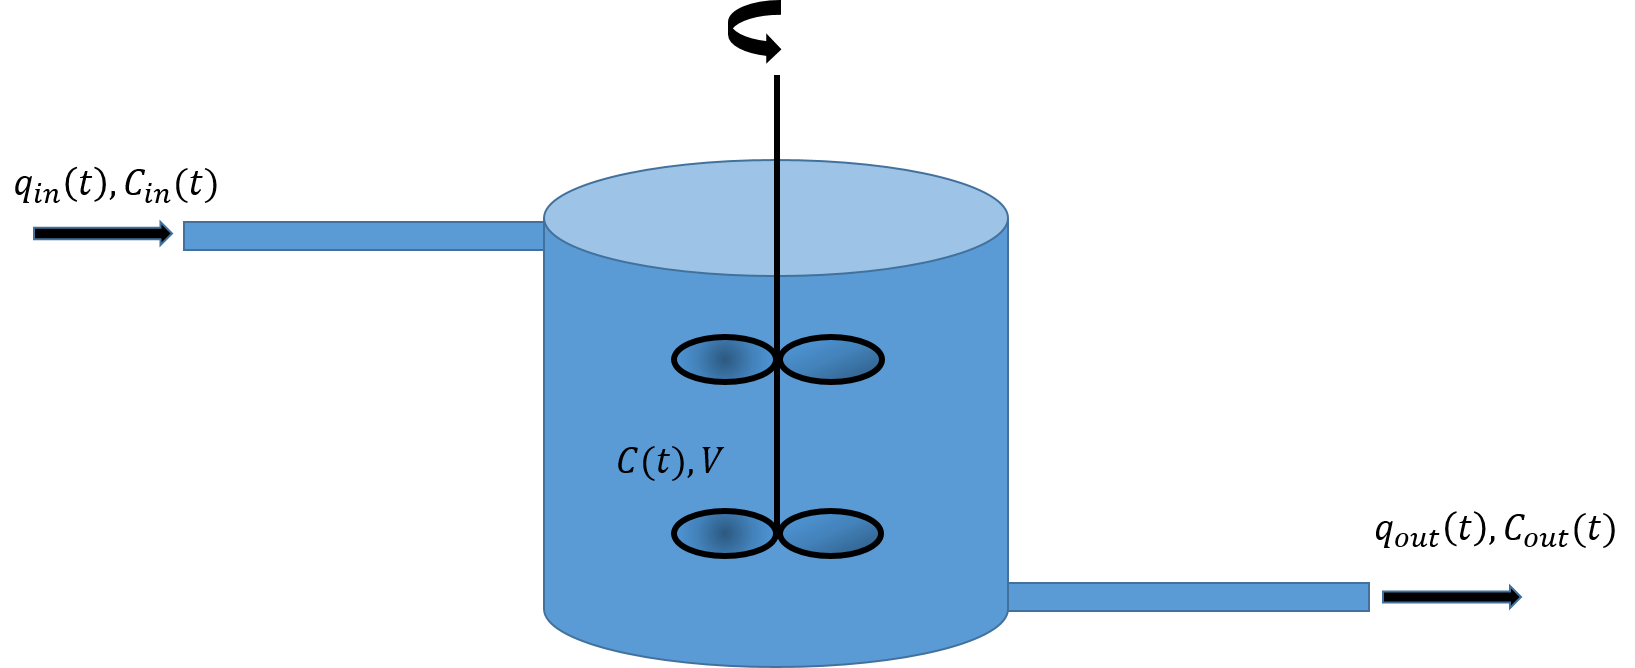
\includegraphics[width=0.9\linewidth]{fig-ode/cstr.png}}
  \caption{
  A continuous stirred tank model, $C(t)=C_\text{out}(t)$, and $q_\text{out}=q_\text{in}$. \label{fig:ode:cstr}
  }
\end{figure}
%\clearpage % flush figures fig:ode:cstr

The concentration $C$ is measured in gram of salt per liter water, and the flow rate $q$ is liter of water per day. The model for the salt balance in this system can be described in words by:
\begin{align}
[\text{accumulation of salt}] &= [\text{salt into the system}] - [\text{salt out of the system}]\nonumber\\ 
& + [\text{generation of salt}].\label{eq:ode:mbal}
\end{align}
In our case there are no generation of salt within the system so this term is zero. The flow of salt into the system during a time $\Delta t$ is: 
$q_\text{in}(t)\cdot C_\text{in}(t)\cdot \Delta t=q(t)\cdot C_\text{in}(t)\cdot \Delta t$, 
the flow of salt out of the system is: $q_\text{out}(t)\cdot C_\text{out}(t)\cdot \Delta t=q(t)\cdot C(t)\cdot \Delta t$, and the accumulation during a time step is:
$C(t+\Delta t)\cdot V - C(t)\cdot V$, hence:
\begin{equation}
C(t+\Delta t)\cdot V - C(t)\cdot V = q(t)\cdot C_\text{in}(t)\cdot \Delta t - q(t)\cdot C(t)\cdot \Delta t.\label{eq:ode:cstr1}
\end{equation}
Note that it is not a priori apparent, which time the concentrations and flow rates on the right hand side should be evaluated at, 
we could have chosen to evaluate them at $t+\Delta t$, or at any time $t\in [t,t+\Delta t]$. We will return to this point later in this chapter. Dividing by $\Delta t$, and taking the limit
$\Delta t\to 0$, we can write equation (\ref{eq:ode:cstr1}) as:
\begin{equation}
V\frac{dC(t)}{dt} = q(t)\left[C_\text{in}(t) - C(t)\right].\label{eq:ode:cstr2}
\end{equation}
Seawater contains about 35 gram salt/liter fluid, if we assume that the fresh water contains no salt, we have the boundary conditions
$C_\text{in}(t)=0$, $C(0)=$35gram/l. The equation (\ref{eq:ode:cstr2}) the reduces to:
\begin{equation}
V\frac{dC(t)}{dt} = -qC(t),\label{eq:ode:cstr3}
\end{equation}
this equation can easily be solved, by dividing by $C$, multiplying by $dt$ and integrating:
\begin{align}
V\int_{C_0}^C\frac{dC}{C} &= -q\int_0^tdt,\nonumber\\ 
C(t)&=C_0e^{-t/\tau},\text{ where } \tau\equiv \frac{V}{q}.\label{eq:ode:sol}
\end{align}
This equation can be inverted to give $t=-\tau\ln[C(t)/C]$. If we assume that the volume of the tank is 1m$^3$=1000liters, 
and that the flow rate is 1 liter/min, we find that $\tau$=1000min=0.69days and that it takes about $-0.69\ln0.9\simeq1.6$days to reduce the concentration
by 90$\%$ to 3.5 gram/liter.     



\begin{graybox2admon}[The CSTR]
You might think that the CSTR is a very simple model, and it is, but this type of model is the basic building blocks in chemical engineering.
By putting CSTR tanks in series and/or connecting them with pipes, the efficiency of manufacturing various type of chemicals
can be investigated. Although the CSTR is an idealized model for the part of a chemical factory, it is actually a \emph{very good} model 
for fluid flow in a porous media. By connecting CSTR tanks in series, one can model how chemical tracers propagate in the subsurface. 
The physical reason for this is that dispersion in porous media will play the role of the propellers and mix the concentration
uniformly.
\end{graybox2admon}




\section{Euler's method}
\index{Eulers method}
If the system gets slightly more complicated, e.g several tanks in series with a varying flow rate or if salt was generated in the tank, there is a
good chance that we have to solve the equations numerically to obtain a solution.
Actually, we have already developed a numerical algorithm to solve equation (\ref{eq:ode:cstr2}), 
before we arrived at equation (\ref{eq:ode:cstr2}) in equation (\ref{eq:ode:cstr1}). This is a special case of Eulers method, which is basically to 
replace the derivative in equation (\ref{eq:ode:cstr2}), with $(C(t+\Delta t)-C(t))/\Delta t$. By rewriting equation (\ref{eq:ode:cstr1}), so that we
keep everything related to the new time step, $t+\Delta t$, on one side, we get:
\begin{align}
VC(t+\Delta t) &= VC(t) + qC_\text{in}(t) - qC(t),\label{eq:ode:eu0}\\ 
C(t+\Delta t) &= C(t) + \frac{\Delta t}{\tau}\left[C_\text{in}(t) - C(t)\right]\label{eq:ode:eu1},
\end{align}
we introduce the short hand notation: $C(t)=C_n$, and $C(t+\Delta t)=C_{n+1}$, hence the algorithm can be written more compact as:
\begin{equation}
C_{n+1} = \left(1-\frac{\Delta t}{\tau}\right)C_n + \frac{\Delta t}{\tau}C_{\text{in},n}\label{eq:ode:eu2},
\end{equation}
In the script below, we have implemented equation (\ref{eq:ode:eu2}).




















\begin{lstlisting}[language=python,style=blue1]
def analytical(x):
    return np.exp(-x)

def euler_step(c_old, c_in, tau_inv,dt):
    fact=dt*tau_inv
    return (1-fact)*c_old+fact*c_in

def ode_solv(c_into,c_init,t_final,vol,q,dt):
    f=[];t=[]
    tau_inv = q/vol
    c_in    = c_into #freshwater into tank
    c_old   = c_init #seawater present 
    ti=0.
    while(ti <= t_final):
        t.append(ti); f.append(c_old)
        c_new = euler_step(c_old,c_in,tau_inv,dt)     
        c_old = c_new
        ti   += dt
    return t,f

\end{lstlisting}


\begin{figure}[!ht]  % fig:ode:euler
  \centerline{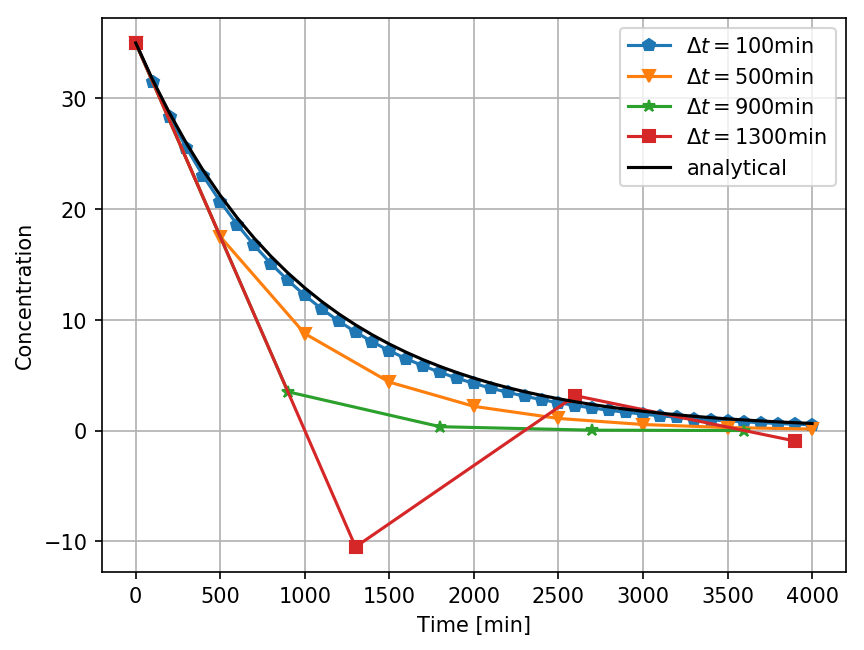
\includegraphics[width=0.9\linewidth]{fig-ode/euler.png}}
  \caption{
  The concentration in the tank for different step size $\Delta t$. \label{fig:ode:euler}
  }
\end{figure}
%\clearpage % flush figures fig:ode:euler

In figure~\ref{fig:ode:euler} the result of the implementation is shown for different values of $\Delta t$.
Clearly we see that the results are dependent on the step size, as the step increases the numerical solution deviates from the analytical solution. At some point the 
numerical algorithm fails completely, and produces results that have no meaning. 

\subsection{Error analysis - Euler's method}
\index{Eulers method, error analysis}
There are two obvious questions:
\begin{enumerate}
\item When does the algorithm produce unphysical results?  

\item What is an appropriate step size? 
\end{enumerate}

\noindent
Let us consider the first question, clearly when the concentrations gets negative the solution is unphysical. From equation (\ref{eq:ode:eu2}), 
we see that when $\Delta t/\tau > 1$, the concentration 
become negative. For this specific case (the CSTR), there is a clear physical interpretation of this condition. Inserting $\tau=V/q$, we can rewrite
the condition $\Delta t/\tau <1$ as $q\Delta t < V$. The volume into the tank during one time step is: $q\Delta t$, which means that
whenever we \emph{flush more than one tank volume through the tank during one time step, the algorithm fails}.
When this happens the new concentration in the tank cannot be predicted from the old one. This makes sense, because we could have switched to a
new solution (e.g.~seawater) during that time step, then the new solution does not have any relation to the old solution. 

The second question, "what is an appropriate step size?",  is a bit more difficult to answer.
One strategy could be to simply use the results from chapter [Taylor], where we showed that the truncation error had a minimum value
with a step size of $10^{-8}$  (when using a first order Taylor approximation).
How does the value $10^{-8}$ relate to the step sizes in minutes used in our Euler implementation?
In order to see the connection, we need to rewrite equation (\ref{eq:ode:cstr2}) in a dimensionless form,
by making the following substitution:
 $t\to t/\tau$:
\begin{equation}
\frac{dC(\tau)}{d\tau} = \left[C_\text{in}(\tau) - C(\tau)\right].\label{eq:ode:cstr2dim}
\end{equation}
As we found earlier $\tau = 1000$min, thus a step size of e.g.~1 min would correspond to a dimensionless time step of 
$\Delta t\to$1min/1000min$=10^{-3}$. This number can be directly compared to the value $10^{-8}$, which is the lowest value we can
choose without getting into trouble with round off errors on the machine. 


\begin{graybox2admon}[Dimensionless variables]
It is a  good idea to formulate our equations in terms of dimensionless variables.
The algorithms we develop can then be used in the same form regardless of changes in the system size and flow rates.
Thus we do not need to rewrite the algorithm each time the physical system changes. This also means that if you use
an algorithm developed by someone else (e.g.~in Matlab or Python), you should always formulate the ODE system in dimensionless form before using the algorithm.

A second reason is that from a pure modeling point of view, dimensionless variables is a way of getting some
understanding of what kind of combination of the physical parameters that describes the behavior of the system.
For the case of the CSTR, there is a time scale $\tau=V/q$, which 
is an intrinsic measure of time in the system. No matter what the flow rate through the tank or the volume of the tank is,
it will always take  0.1$\tau$ before
the concentration in the tank is reduced by 90\%.
\end{graybox2admon}



As already mentioned a step size of $10^{-8}$, is probably the smallest we can choose with respect to round off errors, 
but it is smaller than necessary and would lead to large simulation times. 
If it takes 1 second to run the simulation with a step size of $10^{-3}$, it would take $10^5$ seconds or 1 day
with a step size of $10^{-8}$. 
To continue the error analyses, we write our ODE for a general system as:
\begin{align}
\frac{dy}{dt}=f(y,t),\label{eq:ode:ode}
\end{align}
or in discrete form:
\begin{align}
\frac{y_{n+1}-y_n}{h}-\frac{h}{2}y^{\prime\prime}(\eta_n)&=f(y,t).\nonumber\\ 
y_{n+1}&=y_n+hf(y,t)+\frac{h^2}{2}y^{\prime\prime}(\eta_n).
\end{align}
$h$ is now the (dimensionless) step size, equal to $\Delta t$ if the derivative is with respect to $t$ or $\Delta x$ if the derivative is respect to $x$ etc. Note that we
have also included the error term related to the numerical derivative, $\eta_n\in[t_n,t_n+h]$. At each step we get an error term,
and the distance between the true solution and our estimate, the \emph{local error}, after $N$ steps is:
\begin{align}
\epsilon=\sum_{n=0}^{N-1}\frac{h^2}{2}y^{\prime\prime}(\eta_n)&=\frac{h^2}{2}\sum_{n=0}^{N-1}f^\prime(y_n,\eta_n)\simeq\frac{h}{2}\int_{t_0}^{t_f}f^\prime(y,\eta)d\eta\nonumber\\ 
&=\frac{h}{2}\left[f(y(t_f),t_f)-f(y(t_0),t_0)\right].\label{eq:ode:eu3}
\end{align}
Note that when we replace the sum with an integral in the equation above, this is only correct if the step size is not too large.
From equation (\ref{eq:ode:eu3})
we see that even if the error term on the numerical derivative is $h^2$, the local error is proportional to $h$
(one order lower). This is because we accumulate errors for each step.

In the following we specialize to the CSTR, to see if we can gain some additional insight. First we change variables in 
equation (\ref{eq:ode:cstr3}): $y=C(t)/C_0$, and $x=t/\tau$, hence:
\begin{equation}
\frac{dy}{dx}=-y.\label{eq:ode:simple}
\end{equation}
The solution to this equation is $y(x)=e^{-x}$, substituting back for the new variables $y$ and $x$, we reproduce the result in equation (\ref{eq:ode:sol}). 
The local error, equation (\ref{eq:ode:eu3}), reduces to:
\begin{align}
\epsilon=\frac{h}{2}\left[-y(x_f)+y(x_0)\right]=\frac{h}{2}\left[1-e^{-x_f}\right],\label{eq:ode:eu4}
\end{align}
we have assumed that $x_0=t_0/\tau=0$. This gives the estimated local error at time $x_f$. For $x_f=0$, the 
numerical error is zero, this makes sense because at $x=0$ we know the exact solution because of the initial conditions. When we move further away from the initial conditions, the
numerical error increases, but equation (\ref{eq:ode:eu4}) ensures us that as long as the step size is low enough we can get as
close as possible to the true solution, since the error scales as $h$ (at some point we might run into trouble with round off error in the computer).

Can we prove directly that we get the analytical result? In this 
case it is fairly simple, if we use Eulers method on equation (\ref{eq:ode:simple}), we get:
\begin{align}
\frac{y_{n+1}-y_n}{h}&=-y_nf.\nonumber\\ 
y_{n+1}&=(1-h)y_n,
\end{align}
or alternatively:
\begin{align}
y_1&=(1-h)y_0,\nonumber\\ 
y_2&=(1-h)y_1=(1-h)^2y_0,\nonumber\\ 
\vdots\nonumber\\ 
y_{N+1}&=(1-h)^{N}y_0=(1-h)^{x_f/h}y_0.
\end{align}
In the last equation, we have used the the fact the number of steps, $N$, is equal to the simulation time divided by the step size, hence: $N=x_f/h$. From calculus,
the equation above is one of the well known limits for the exponential function: $\lim_{x\to\infty}(1+k/x)^{mx}=e^{mk}$, hence:
\begin{align}
y_n&=(1-h)^{x_f/h}y_0\to e^{-x_f},
\end{align}
when $h\to0$. Below is an implementation of the Euler algorithm in this simple case, we also estimate the local error, and global error after $N$ steps. 


















\begin{lstlisting}[language=python,style=blue1bar]
import matplotlib.pyplot as plt
import numpy as np
def euler(tf,h):
    t=[];f=[]
    ti=0.;fi=1.
    t.append(ti);f.append(fi)
    global_err=0.
    while(ti<= tf):
        ti+=h
        fi=fi*(1-h)
        global_err += abs(np.exp(-ti)-fi)
        t.append(ti);f.append(fi)
    print("error= ", np.exp(-ti)-fi," est.err=", .5*h*(1-np.exp(-ti)))
    print("global error=",global_err)
    return t,f
                                        
t,f=euler(1,1e-5)

\end{lstlisting}

By changing the step size $h$, you can easily verify that the local error systematically increases or decreases proportional to $h$.
Something curious happens with the global error when the 
step size is changed, it does not change very much. The global error involves a second sum over the local error for each step,
which can be approximated as a second integration in equation (\ref{eq:ode:eu4}):
\begin{align}
\epsilon_\text{global}=\frac{1}{2}\int_{0}^{x_f}\left[-y(x)+y(0)\right]dx=\frac{1}{2}\left[x_f+e^{-x_f}-1\right].\label{eq:ode:eu5}
\end{align}
Note that the global error does not go to zero when the step size decreases, which can easily be verified by changing the step size. This is strange, but can be understood
by the following argument: when the step size decreases the local error scales as $\sim h$, but the number of steps scales as $1/h$, so the global error must scale as $h\times 1/h$
or some constant value. Usually it is much easier to control the local error than the global error, this should be kept in mind if you ever encounter a problem where it is 
important control the global error. For the higher order methods that we will discuss later in this chapter, the global error will go to zero when $h$ decreases.   

The answer to our original question, ''What is an appropriate step size?'', will depend on what you want to achieve in terms of local or global error.
In most practical situations you would
specify a local error that is acceptable for the problem under investigation and then choose a step size where the local error always is lower than this value. In the 
next subsection we will investigate how to achieve this in practice.

\subsection{Adaptive step size - Euler's method}
\index{Eulers method, adaptive step size}
We want to be sure that we use a step size that achieves a certain accuracy in our numerical solution, but at
the same time that we do not waste simulation time using a too low step size. The following approach is similar to the one we derived for the Romberg integration, and
a special case of what is known as Richardson Extrapolation. The method is easily extended to higher order methods. 

We know that Eulers algorithm is accurate to second order. Our estimate of the new value, $y_1^*$  
(where we have used a$\,{}^*$ to indicate that we have used a step size of size $h$), should then be related to the true solution $y(t_1)$ in the following way:
\begin{align}
y^*_1=y(t_1)+ch^2.\label{eq:ode:aeb0}
\end{align}
The constant $c$ is unknown, but it can be found by taking two smaller steps of size $h/2$. If the steps are not too large, our new estimate
of the value $y_1$ will be related to the true solution as:
\begin{align}
y_1=y(t_1)+2c\left(\frac{h}{2}\right)^2.\label{eq:ode:aeb1}
\end{align}
The factor 2 in front of $c$ is because we now need to take two steps, and we accumulate a total error of $2c(h/2)^2=ch^2/2$. It might not be completely 
obvious that the constant $c$ should be the same in equation (\ref{eq:ode:aeb0}) and (\ref{eq:ode:aeb1}). If you are not convinced, there is an exercise at the end 
of the chapter.  
We define:
\begin{align}
\Delta\equiv y^*_1-y_1=c\frac{h^2}{2}.\label{eq:ode:ae5}
\end{align}
The truncation error in equation (\ref{eq:ode:aeb1}) is:
\begin{align}
\epsilon=y(t_1)-y_1=2c\left(\frac{h}{2}\right)^2=\Delta.\label{eq:ode:ae5b}
\end{align}
Now we have everything we need: We want the local error to be smaller than some predefined
tolerance, $\epsilon^\prime$, or equivalently 
that $\epsilon\le\epsilon^\prime$. 
To achieve this we need to use an optimal step size, $h^\prime$,  that gives us exactly the desired error:
\begin{align}
\epsilon^\prime=c\frac{{h^\prime}^2}{2}.\label{eq:ode:ae6}
\end{align}
Dividing equation (\ref{eq:ode:ae6}) by equation (\ref{eq:ode:ae5b}), we can estimate the optimal step size:
\begin{align}
h^\prime=h\sqrt{\left|\frac{\epsilon^\prime}{\epsilon}\right|},\label{eq:ode:ae7}
\end{align}
where the estimated error, $\epsilon$, is calculated from equation (\ref{eq:ode:ae5b}).
Equation (\ref{eq:ode:ae7}) serves two purposes, if the estimated error $\epsilon$ is higher than the tolerance, $\epsilon^\prime$, we have specified it will 
give us an estimate for the step size we should choose in order to achieve a higher accuracy, if on the other hand $\epsilon^\prime > \epsilon$, then we 
get an estimate for the next, larger step. Before the implementation we note, as we did for the Romberg integration, that equation (\ref{eq:ode:ae5b}) 
also gives us an estimate for the error term in equation (\ref{eq:ode:aeb1}) as an improved estimate of $y_1$. This we get for
free and will make our Euler algorithm accurate to $h^3$, hence the improved Euler step, $\hat{y_1}$, is to \emph{subtract} the error
term from our previous estimate:
\begin{align}
\hat{y_1}=y_1-\epsilon=2y_1-y_1^*.
\end{align}
Below is an implementation of the adaptive Euler algorithm:































\begin{lstlisting}[language=python,style=blue1]
def one_step(c_old, c_in,h):
    return (1-h)*c_old+h*c_in

def adaptive_euler(c_into,c_init,t_final,tol=1e-4):
    f=[];t=[]
    c_in    = c_into #freshwater into tank
    c_old   = c_init #seawater present 
    ti=0.; h_new=1e-3;
    no_steps=0
    global_err=0.
    while(ti <= t_final):
        t.append(ti); f.append(c_old)
        toli=10.*tol; # a high init tolerance to enter while loop
        while(toli>tol):# first two small steps
            hi=h_new
            k1 = one_step(c_old,c_in,hi*.5)
            k2 = one_step(k1,c_in,hi*.5)
            # ... and one large step
            k3 = one_step(c_old,c_in,hi)
            toli = abs(k3-k2)
            h_new=hi*np.sqrt(tol/toli)
            no_steps+=3
        toli=1.
        c_old=2*k2-k3 # higher order correction
 # normal Euler, uncomment and inspect the global error
 #       c_old = k2 
        ti   += hi
        global_err += abs(np.exp(-ti)-c_old)
    print("No steps=", no_steps, "Global Error=", global_err)
    return t,f

\end{lstlisting}


\begin{figure}[!ht]  % fig:ode:adapt_euler
  \centerline{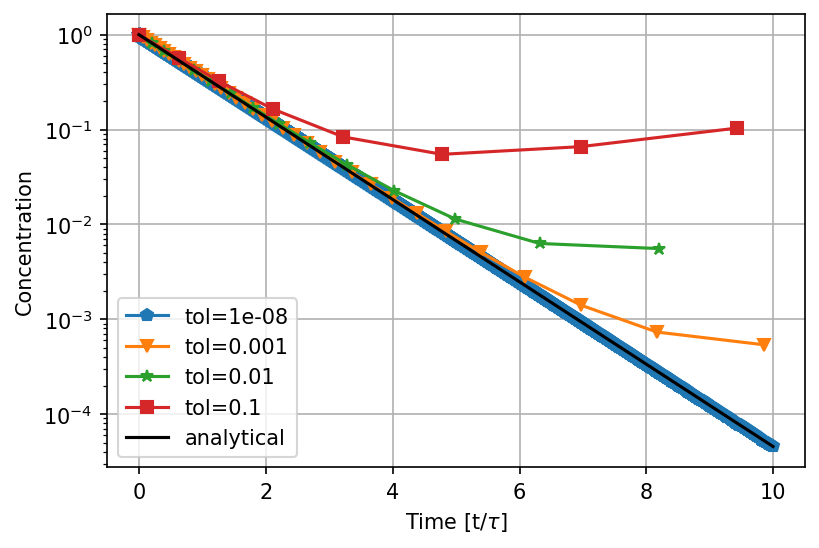
\includegraphics[width=0.9\linewidth]{fig-ode/adaptive_euler.png}}
  \caption{
  The concentration in the tank using adaptive Euler. Number of Euler steps are: 3006, 117, 48 and 36 for the different step sizes. \label{fig:ode:adapt_euler}
  }
\end{figure}
%\clearpage % flush figures fig:ode:adapt_euler

In figure~\ref{fig:ode:adapt_euler} the result of the implementation is shown. 
Note that the number of steps for an accuracy of $10^{-6}$ is only about 3000. Without knowing anything about the accuracy, we would have to assume
that we needed a step size of the order of $h$ in order to reach a local accuracy of $h$ because of equation (\ref{eq:ode:eu3}). In the current case,
we would have needed $10^7$ steps, which would lead to unnecessary long simulation times.


\begin{graybox2admon}[Local error and bounds]
In the previous example we set an absolute tolerance, and required that our estimate $y_n$ always is within a certain bound
of the true  solution $y(t_n)$, i.e.~$|y(t_n)-y_n|\le\epsilon^\prime$. This is a very strong demand, and sometimes it makes more 
sense to require that we also accept a relative tolerance proportional to function value. In some areas the solution might have a very large
value, and then another possibility would be to have an $\epsilon^\prime$ that varied with the function value: $\epsilon^\prime = atol +|y|rtol$, where 'atol' is the absolute tolerance and 'rtol' is the relative tolerance. A sensible choice would be to set 'atol=rtol' (e.g. = $10^{-4}$).
\end{graybox2admon}




\section{Runge-Kutta methods}
\index{Runge-Kutta}

\begin{figure}[!ht]  % fig:ode:rk
  \centerline{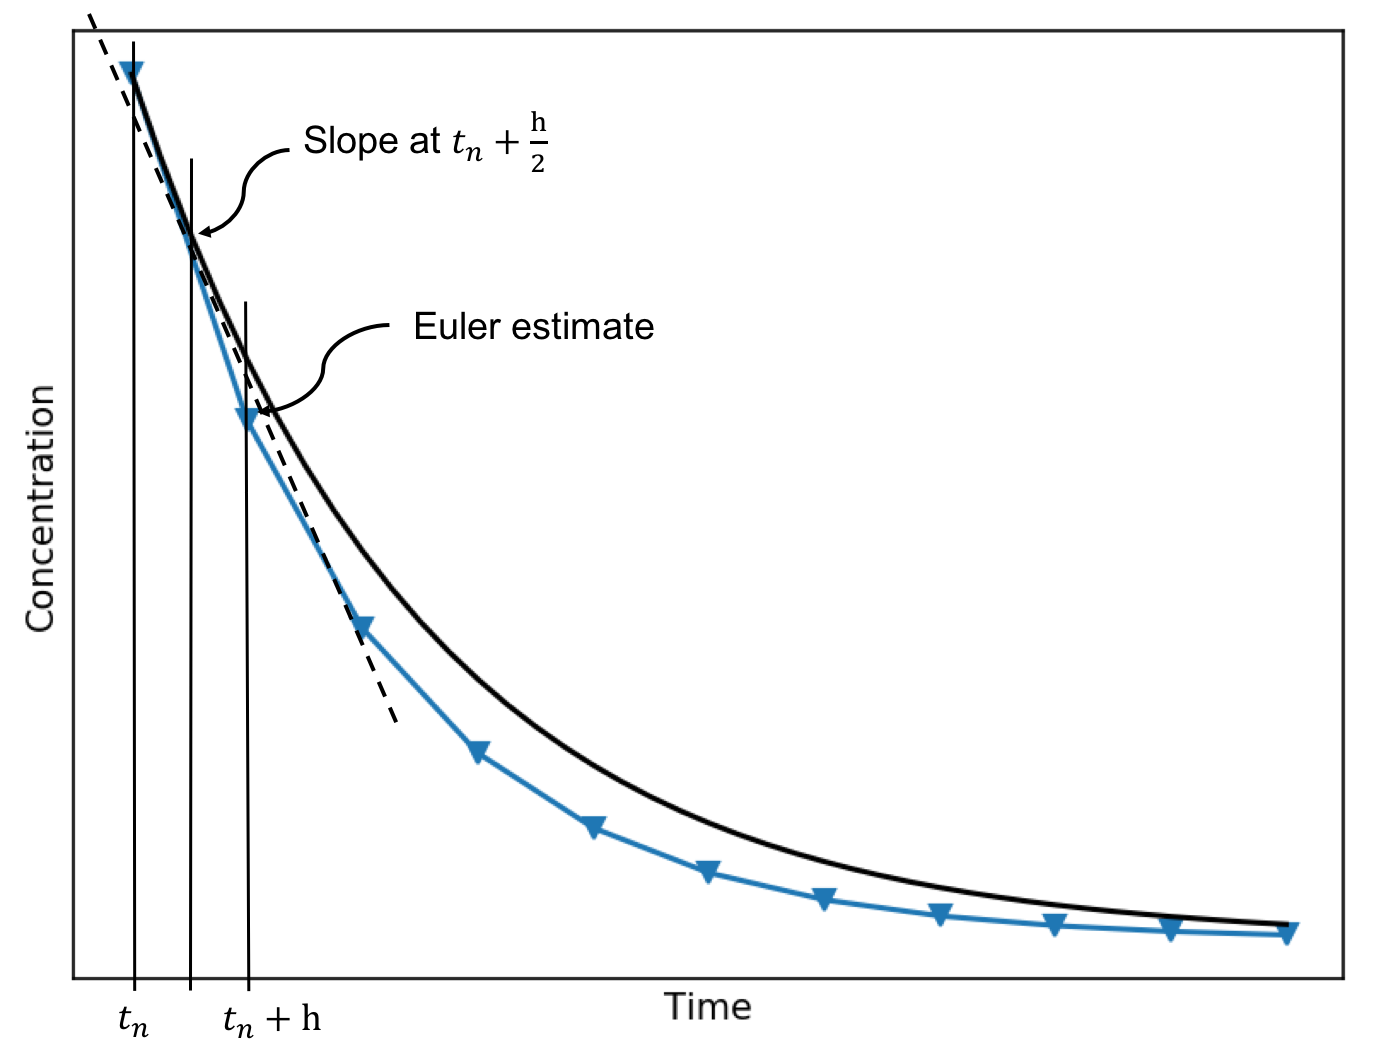
\includegraphics[width=0.9\linewidth]{fig-ode/rk_fig.png}}
  \caption{
  Illustration of the Euler algorithm, and a motivation for using the slope a distance from the $t_n$.\label{fig:ode:rk}
  }
\end{figure}
%\clearpage % flush figures fig:ode:rk

The Euler method only have an accuracy of order $h$, and a global error that do not go to zero as the step size decrease. 
The Runge-Kutta methods may be motivated by inspecting the Euler method in figure~\ref{fig:ode:rk}. The Euler method uses information from
the previous time step to estimate the value at the new time step. The Runge Kutta methods uses the information about the slope between the
points $t_n$ and $t_n+h$. By inspecting figure~\ref{fig:ode:rk}, we clearly see that by using the slope at $t_n+h/2$ would give us a
significant improvement. The 2. order Runge-Kutta method can be derived by Taylor expanding the solution around $t_n+h/2$, we do this by
setting $t_n+h=t_n+h/2+h/2$:
\begin{align}
y(t_n+h)=y(t_n+\frac{h}{2})+\frac{h}{2}\left.\frac{dy}{dt}\right|_{t=t_n+h/2}+\frac{h^2}{4}\left.\frac{d^2y}{dt^2}\right|_{t=t_n+h/2}
+\mathcal{O}(h^3).\label{eq:ode:rk1}
\end{align}
Similarly we can expand the solution in $y(t_n)$ about $t_n+h/2$, by setting $t_n=t_n+h/2-h/2$:
\begin{align}
y(t_n)=y(t_n+\frac{h}{2})-\frac{h}{2}\left.\frac{dy}{dt}\right|_{t=t_n+h/2}+\frac{h^2}{4}\left.\frac{d^2y}{dt^2}\right|_{t=t_n+h/2}
-\mathcal{O}(h^3).\label{eq:ode:rk2}
\end{align}
Subtracting these two equations the term $y(t_n+\frac{h}{2})$, and all even powers in the derivative cancels out:
\begin{align}
y(t_n+h)&=y(t_n)+h\left.\frac{dy}{dt}\right|_{t=t_n+h/2}+\mathcal{O}(h^3),\nonumber\\ 
y(t_n+h)&=y(t_n)+hf(y_{n+h/2},t_n+h/2)+\mathcal{O}(h^3).\label{eq:ode:rk3}
\end{align}
In the last equation, we have used equation (\ref{eq:ode:ode}). Note that we now have an expression that is very similar to Eulers algorithm,
but it is accurate to order $h^3$. There is one problem, and that is that the function $f$ is to be evaluated at the point $y_{n+1/2}=y(t_n+h/2)$
which we do not know. This can be fixed by using Eulers algorithm: $y_{n+1/2}=y_n+h/2f(y_n,t_n)$. We can do this even if Eulers algorithm has an error term of order $h^2$, because the $f$ in equation (\ref{eq:ode:rk3}) is multiplied by $h$, and thus our algorithm is still has an error term of order $h^3$. 


\begin{graybox2admon}[The 2. order Runge-Kutta:]
\begin{align}
k_1&=hf(y_n,t_n)\nonumber\\ 
k_2&=hf(y_n+\frac{1}{2}k_1,t_n+h/2)\nonumber\\ 
y_{n+1}&=y_n+k_2\label{eq:ode:rk4}
\end{align}
\end{graybox2admon}



Below is a Python implementation of equation (\ref{eq:ode:rk4}):




















\begin{lstlisting}[language=python,style=blue1]
def fm(c_old,c_in):
    return c_in-c_old

def rk2_step(c_old, c_in, h):
    k1=h*fm(c_old,c_in)
    k2=h*fm(c_old+0.5*k1,c_in)
    return c_old+k2

def ode_solv(c_into,c_init,t_final,h):
    f=[];t=[]
    c_in  = c_into #freshwater into tank
    c_old = c_init #seawater present 
    ti=0.
    while(ti <= t_final):
        t.append(ti); f.append(c_old)
        c_new = rk2_step(c_old,c_in,h)     
        c_old = c_new
        ti   += h
    return t,f

\end{lstlisting}


\begin{figure}[!ht]  % fig:ode:rk2
  \centerline{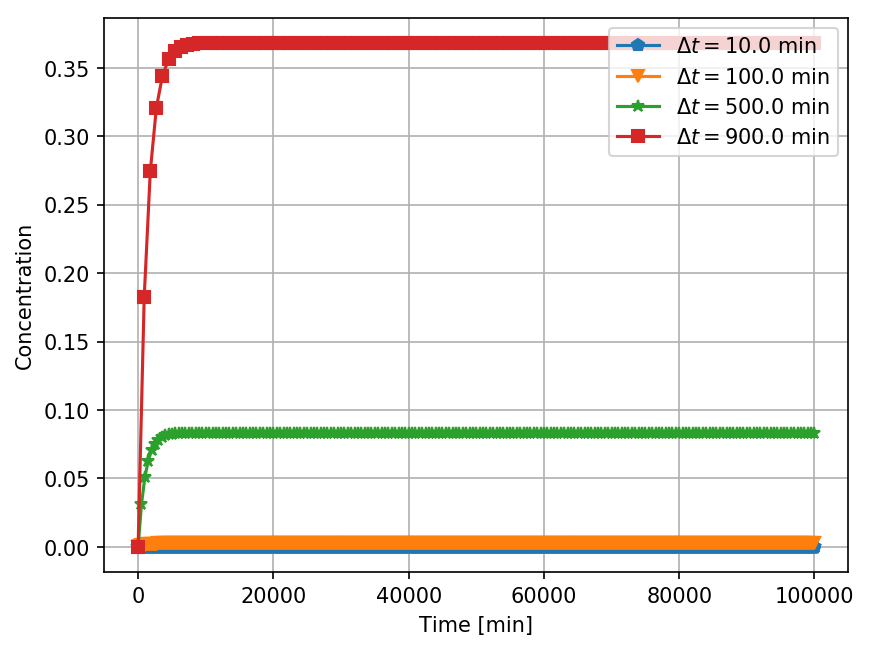
\includegraphics[width=0.9\linewidth]{fig-ode/rk2.png}}
  \caption{
  The concentration in the tank for different step size $\Delta t$. \label{fig:ode:rk2}
  }
\end{figure}
%\clearpage % flush figures fig:ode:rk2

In figure~\ref{fig:ode:rk2} the result of the implementation is shown. 
Note that when comparing Runge-Kutta 2. order with Eulers method,
see figure~\ref{fig:ode:rk2} and~\ref{fig:ode:euler},
we of course have 
the obvious result that a larger step size can be taken, without loosing numerical accuracy. It is also worth noting that we can take steps that
is larger than the tank volume. Eulers method failed whenever the time step was larger than one tank volume ($h=t/\tau>1$), whereas the Runge-Kutta 
method finds a physical solution for step sizes lower than twice the tank volume. If the step size is larger, we see that the concentration in the tank
increases, which is clearly unphysical. 

The Runge-Kutta fourth order method is one of he most used methods, it is accurate to order $h^4$, and has an error of order $h^5$. The development of the 
algorithm itself is similar to the 2. order method, but of course more involved. We just quote the result:


\begin{graybox2admon}[The 4. order Runge-Kutta:]
\begin{align}
k_1&=hf(y_n,t_n)\nonumber\\ 
k_2&=hf(y_n+\frac{1}{2}k_1,t_n+h/2)\nonumber\\ 
k_3&=hf(y_n+\frac{1}{2}k_2,t_n+h/2)\nonumber\\ 
k_4&=hf(y_n+k_3,t_n+h)\nonumber\\ 
y_{n+1}&=y_n+\frac{1}{6}(k_1+2k_2+2k_3+k_4)\label{eq:ode:rk5}
\end{align}
\end{graybox2admon}



In figure~\ref{fig:ode:rk4} the result of the Runge-Kutta fourth order is shown, by comparing it to figure~\ref{fig:ode:rk2} it is easy to see that a larger step size can be chosen.     
% Below is a Python implementation of equation (\ref{eq:ode:rk5}):
% @@@CODE src-ode/rk4.py  fromto: def fm@# rest

\begin{figure}[!ht]  % fig:ode:rk4
  \centerline{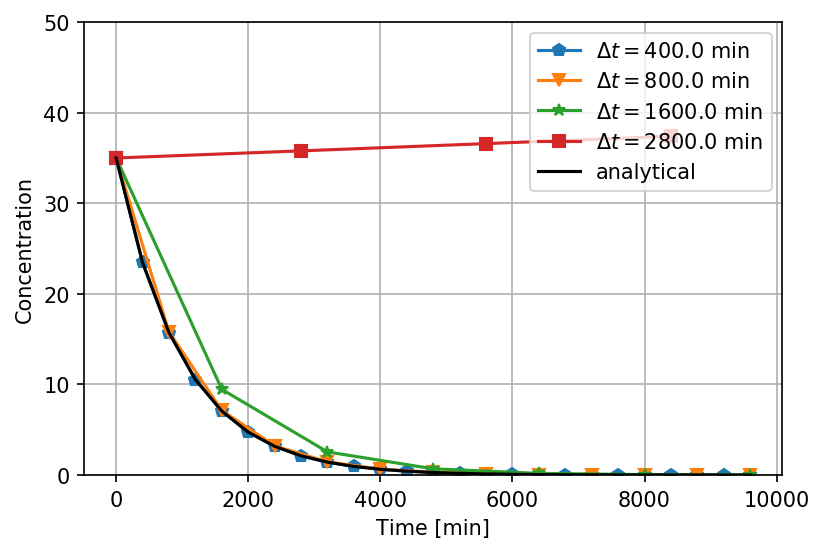
\includegraphics[width=0.9\linewidth]{fig-ode/rk4.png}}
  \caption{
  The concentration in the tank for different step size $\Delta t$. \label{fig:ode:rk4}
  }
\end{figure}
%\clearpage % flush figures fig:ode:rk4

% % endif

\subsection{Adaptive step size - Runge-Kutta method}
\index{Runge-Kutta, adaptive step size}
Just as we did with Eulers method, we can implement an adaptive method. The derivation is exactly the same, but this time our method is accurate to
fourth order, hence the error term is of order $h^5$. We start by taking one large step of size $h$, our estimate, $y_1^*$ is related to the true 
solution, $y(t_1)$, in the following way:
\begin{align}
y^*_1&=y(t_1)+ch^5,\label{eq:ode:rka0}
\end{align}
Next, we take two steps of half the size, $h/2$, hence:
\begin{align}
y_1&=y(t)+2c\left(\frac{h}{2}\right)^5.\label{eq:ode:rka1}
\end{align}
Subtracting equation (\ref{eq:ode:rka0}) and (\ref{eq:ode:rka1}), we find an expression similar to equation (\ref{eq:ode:ae5}):
\begin{align}
\Delta\equiv& y_1^*-y_1=c\frac{15}{16}h^5,\label{eq:ode:rka2}
\end{align}
or $c=16\Delta/(15h^5)$. For the Euler scheme, $\Delta$ also happened to be equal to the truncation error, but in this case it is:
\begin{align}
\epsilon=2c\left(\frac{h}{2}\right)^5=\frac{\Delta}{15}\label{eq:ode:rka5}
\end{align}
we want the local error, $\epsilon$, to be smaller than some tolerance, $\epsilon^\prime$.  
The optimal step size, $h^\prime$,  that gives us exactly the desired error is then:
\begin{align}
\epsilon^\prime=2c\left(\frac{{h^\prime}}{2}\right)^5.\label{eq:ode:rka3}
\end{align}
Dividing equation (\ref{eq:ode:rka3}) by equation (\ref{eq:ode:rka5}), we can estimate the optimal step size:
\begin{align}
h^\prime=h\left|\frac{\epsilon}{\epsilon}\right|^{1/5},\label{eq:ode:rka4}
\end{align}
$\epsilon$ can be calculated from equation (\ref{eq:ode:rka5}). In figure~\ref{fig:ode:adaptive_rk4} the result of an  implementation is shown (see the exercises). 
% Below is an implementation
% % if FORMAT == 'ipynb':
% Run the script below and inspect the results.
% @@@CODE src-ode/rk4.py
% % endif
% % if FORMAT != 'ipynb':
% @@@CODE src-ode/adaptive_rk4.py  fromto: def fm@# rest

\begin{figure}[!ht]  % fig:ode:adaptive_rk4
  \centerline{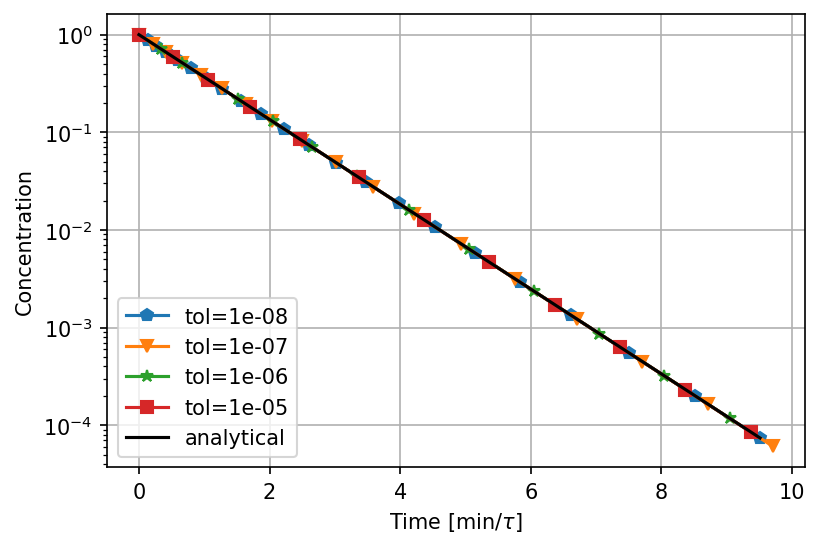
\includegraphics[width=0.9\linewidth]{fig-ode/adaptive_rk4.png}}
  \caption{
  The concentration in the tank for different step size $\Delta t$. Number of rk4 steps are: 138, 99, 72 and 66 for the different step sizes and 'rtol=0', for 'rtol=tol' the number of rk4 steps are 81, 72, 63, 63.\label{fig:ode:adaptive_rk4}
  }
\end{figure}
%\clearpage % flush figures fig:ode:adaptive_rk4

% % endif

In general we can use the same procedure any method accurate to order $h^p$, and you can easily verify that:


\begin{graybox2admon}[Error term and step size for a $h^p$ method:]
\index{adaptive step size}
\begin{align}
|\epsilon|&=\frac{|\Delta|}{2^p-1}=\frac{|y_1^*-y_1|}{2^p-1},\label{eq:eode:1}\\ 
h^\prime&=\beta h\left|\frac{\epsilon}{\epsilon_0}\right|^{\frac{1}{p+1}},\label{eq:eode:2}\\ 
\hat{y_1}&=y_1-\epsilon=\frac{2^p y_1-y_1^*}{2^{p}-1}\label{eq:eode:3},
\end{align}
where $\beta$ is a safety factor $\beta\simeq0.8,0.9$, and you should always be careful that the step size do not become too large so that
the method breaks down. This can happens when $\epsilon$ is very low, which may happen if $y_1^*\simeq y_1$ and/or if $y_1^*\simeq y_1\simeq 0$.
\end{graybox2admon}




\subsection{Conservation of mass}
A mathematical model of a physical system should always be formulated in such a way that it is
consistent with the laws of nature. In practical situations this statement is usually equivalent to state that
the mathematical model should respect conservation laws. The conservation laws can be conservation of mass, energy, momentum, 
electrical charge, etc. In our
example with the mixing tank, we were able to derive an expression for the concentration of salt out of
the tank, equation (\ref{eq:ode:sol}), by \emph{demanding} conservation of mass (see equation (\ref{eq:ode:cstr1})).

A natural question to ask is then: If our mathematical model respect conservation of mass, are we sure that our 
solution method respect conservation of mass? We of course expect that
when the grid spacing approaches zero our numerical solution will get closer and closer to the analytical
solution. Clearly when $\Delta x\to 0$, the mass is conserved. So what is the problem? The problem is that in many practical problems
we cannot always have a step size that is small enough to ensure that our solution always is close enough to the analytical 
solution. The physical system we consider might be very complicated (e.g.~a model for the earth climate), and our ODE system could
be a very small part of a very big system. A very good test of any code is to investigate if the code respect
the conservation laws. If we know that our implementation respect e.g.~mass conservation at the discrete level, we can easily
test mass conservation by summing up all the mass entering, and subtracting the mass out of and present in our system.
If the mass is not conserved exactly, there is a good chance that there is a bug in our implementation.

If we now turn to our system, we know that the total amount of salt in the system when we start is $C(0)V$.
The amount entering is zero, and the amount leaving each time step is $q(t)C(t)\Delta t$. Thus we should
expect that if we add the amount of salt in the tank to the amount that has left the system
we should always get an amount that is equal to the original amount. Alternatively, we expect
$\int_{t_0}^t qC(t)dt + C(t)V -C(0)V=0$. Adding the following code in the \Verb!while(ti <= t_final):! loop:



\begin{lstlisting}[language=python,style=blue1]
mout += 0.5*(c_old+c_new)*q*dt
mbal  = (c_new*vol+mout-vol*c_init)/(vol*c_init)

\end{lstlisting}

it is possible to calculate the amount of mass lost (note that we have used the
trapezoidal formula to calculate the integral). In the table below the fraction of mass lost relative to the original
amount is shown for the various numerical methods.



{\small   % for Springer style: small table font and more vspace

\vspace{4mm}

\begin{tabular}{ccccc}
\hline
\multicolumn{1}{c}{ $\Delta t$ } & \multicolumn{1}{c}{ $h$ } & \multicolumn{1}{c}{ Euler } & \multicolumn{1}{c}{ RK 2. order } & \multicolumn{1}{c}{ RK 4. order } \\
\hline
900         & 0.9  & -0.4500 & 0.3682      & 0.0776      \\
500         & 0.5  & -0.2500 & 0.0833      & 0.0215      \\
100         & 0.1  & -0.0500 & 0.0026      & 0.0008      \\
10          & 0.01 & -0.0050 & 2.5E-05     & 8.3E-06     \\
\hline
\end{tabular}

\vspace{4mm}

}


\noindent
We clearly see from the table that the Runge-Kutta methods performs better than Eulers method, but
\emph{all of the methods violates mass balance}. 

This might not be a surprise as we know that our numerical solution is always an approximation to the analytical solution. How can 
we then formulate an algorithm that will respect conservation laws at the discrete level? It turns out that for Eulers method it is not
so difficult. Eulers algorithm at the discrete level (see equation (\ref{eq:ode:eu0})) is actually a two-step process: first we inject the fresh water while we remove the ``old`` fluid \emph{and then we mix}. By thinking about the
problem this way, it makes more sense to calculate the mass out of the tank as $\sum_kq_kC_k\Delta t_k$. If we in our implementation calculates the mass out of the tank as:



\begin{lstlisting}[language=python,style=blue1]
mout += c_old*q*dt
mbal  = (c_new*vol+mout-vol*c_init)/(vol*c_init)

\end{lstlisting}

We easily find that the mass is exactly conserved at every time for Eulers method. The concentration in the tank will of course not be any closer to the 
analytical solution, but if our mixing tank was part of a much bigger system we could make sure that the mass would always be conserved if we make
sure that the mass out of the tank and into the next part of the system was equal to $qC(t)\Delta t$. 

\section{Solving a set of ODE equations}
What happens if we have more than one equation that needs to be solved? If we continue with our current example, we might be interested in what would happen 
if we had multiple tanks in series. This could be a very simple model to describe the cleaning  of a salty lake by injecting fresh water into it, but at 
the same time this lake was connected to two nearby fresh water lakes, as illustrated in figure~\ref{fig:ode:cstr3}. The weakest part of the model is the assumption about 
complete mixing, in a practical situation we could enforce complete mixing with the salty water in the first tank by injecting fresh water at multiple point in the 
lake. For the two next lakes, the degree of mixing is not obvious, but salt water is heavier than fresh water and therefore it would sink and mix with the fresh water. Thus
if the flow rate was slow, one might imaging that a more or less complete mixing could occur. Our model then could answer questions like, how long time would it take before most
of the salt water is removed from the first lake, and how much time would it take before most of the salt water was cleared from the whole system? The answer to 
these questions would give practical input on how much and how fast one should inject the fresh water to clean up the system. If we had 
data from an actual system, we could compare our model predictions with data from the physical system, and investigate if our model description was correct. 

\begin{figure}[!ht]  % fig:ode:cstr3
  \centerline{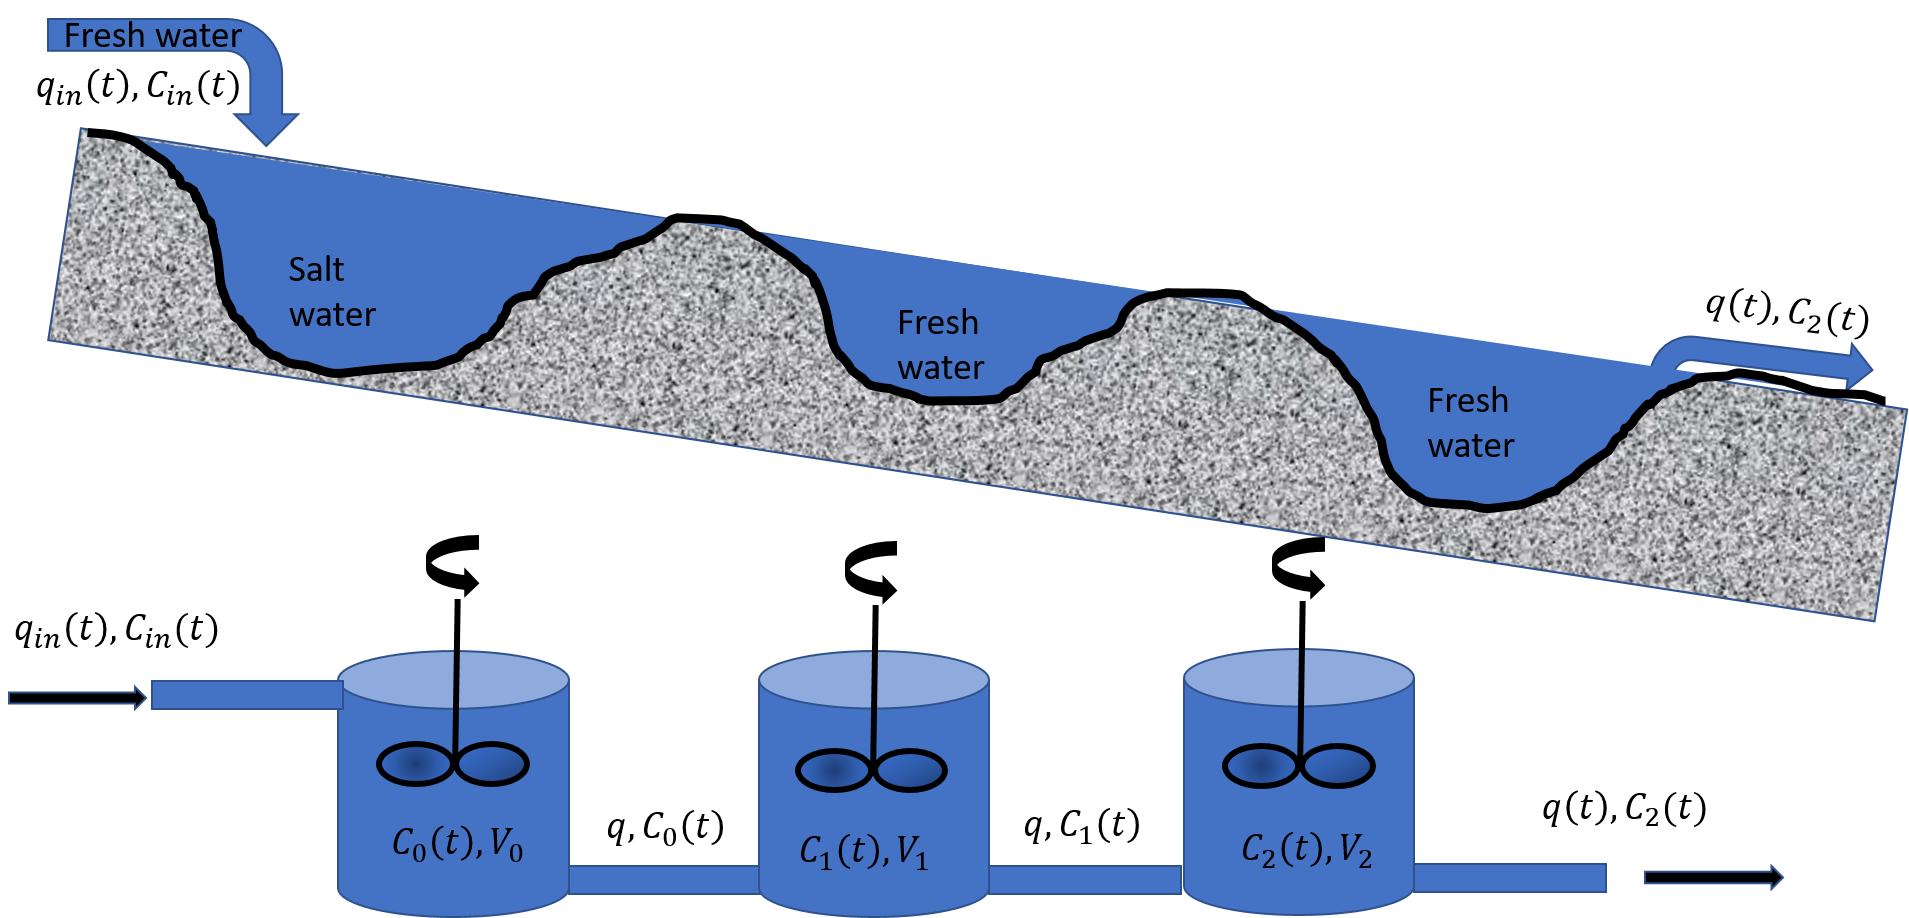
\includegraphics[width=0.9\linewidth]{fig-ode/cstr3.png}}
  \caption{
  A simple model for cleaning a salty lake that is connected to two lakes down stream. \label{fig:ode:cstr3}
  }
\end{figure}
%\clearpage % flush figures fig:ode:cstr3

For simplicity we will assume that all the lakes have the same volume, $V$. The governing equations follows
as before, by assuming mass balance (equation (\ref{eq:ode:mbal})):
\begin{align}
C_0(t+\Delta t)\cdot V - C_0(t)\cdot V &= q(t)\cdot C_\text{in}(t)\cdot \Delta t - q(t)\cdot C_0(t)\cdot \Delta t,\nonumber\\ 
C_1(t+\Delta t)\cdot V - C_1(t)\cdot V &= q(t)\cdot C_0(t)\cdot \Delta t - q(t)\cdot C_1(t)\cdot \Delta t,\nonumber\\ 
C_2(t+\Delta t)\cdot V - C_2(t)\cdot V &= q(t)\cdot C_1(t)\cdot \Delta t - q(t)\cdot C_2(t)\cdot \Delta t.\label{eq:ode:cstr3a}
\end{align}
Taking the limit $\Delta t\to 0$, we can write equation (\ref{eq:ode:cstr3a}) as:
\begin{align}
V\frac{dC_0(t)}{dt} &= q(t)\left[C_\text{in}(t) - C_0(t)\right],\label{eq:ode:cstr3b}\\ 
V\frac{dC_1(t)}{dt} &= q(t)\left[C_0(t) - C_1(t)\right],\label{eq:ode:cstr3c}\\ 
V\frac{dC_2(t)}{dt} &= q(t)\left[C_1(t) - C_2(t)\right].\label{eq:ode:cstr3d}
\end{align}
Let us first derive the analytical solution: Only the first tank is filled with salt water $C_0(0)=C_{0,0}$, $C_1(0)=C_2(0)=0$, and $C_\text{in}=0$. 
The solution to equation (\ref{eq:ode:cstr3b}) is, as before $C_0(t)=C_{0,0}e^{-t/\tau}$, inserting this equation into equation (\ref{eq:ode:cstr3c}) we find:
\begin{align}
V\frac{dC_1(t)}{dt} &= q(t)\left[C_{0,0}e^{-t/\tau} - C_1(t)\right]\label{eq:ode:cstr3e},\\ 
\frac{d}{dt}\left[e^{t/\tau}C_1\right]&= \frac{C_{0,0}}{\tau}\label{eq:ode:cstr3f},\\ 
C_1(t)&=\frac{C_{0,0}t}{\tau}e^{-t/\tau}\label{eq:ode:cstr3g}.
\end{align}
where we have use the technique of \href{{https://en.wikipedia.org/wiki/Integrating_factor}}{integrating factors}\footnote{\texttt{https://en.wikipedia.org/wiki/Integrating\_factor}} when going from equation (\ref{eq:ode:cstr3e}) to (\ref{eq:ode:cstr3f}). 
Inserting equation (\ref{eq:ode:cstr3g}) into equation (\ref{eq:ode:cstr3d}), solving the equation in a similar way as for $C_1$ we find:
\begin{align}
V\frac{dC_2(t)}{dt} &= q(t)\left[\frac{C_{0,0}t}{\tau}e^{-t/\tau} - C_2(t)\right],\label{eq:ode:cstr3h}\\ 
\frac{d}{dt}\left[e^{t/\tau}C_2\right]&= \frac{C_{0,0}t}{\tau},\label{eq:ode:cstr3i}\\ 
C_2(t)&=\frac{C_{0,0}t^2}{2\tau^2}e^{-t/\tau}.\label{eq:ode:cstr3j}
\end{align}
The numerical solution follows the exact same pattern as before if we introduce a vector notation. Before doing that, we rescale the time $t\to t/\tau$ and the concentrations,
 $\hat{C_i}=C_i/C_{0,0}$ for $i=0,1,2$, hence:
\begin{align}
\frac{d}{dt}
\left(
\begin{array}{c} 
 \hat{C_0}(t)\\ 
 \hat{C_1}(t)\\ 
 \hat{C_2}(t)
 \end{array}
 \right)
&=\left(
\begin{array}{c} 
 \hat{C_\text{in}}(t) - \hat{C_0}(t)\\ 
 \hat{C_0}(t) - \hat{C_1}(t)\\ 
 \hat{C_1}(t) - \hat{C_2}(t)
 \end{array}
 \right),\nonumber
 \\ 
 \frac{d\mathbf{\hat{C}}(t)}{dt}&=\mathbf{f}(\mathbf{\hat{C}},t).
\end{align}

In figure~\ref{fig:ode:rk4_2} results of an implementation using Runge-Kutta 4. order is shown (see exercises for more details).
% Below is an implementation using the Runge Kutta 4. order method:
% % if FORMAT == 'ipynb':
% Run the script below and inspect the results.
% @@@CODE src-ode/rk4_2.py
% % endif
% % if FORMAT != 'ipynb':
% @@@CODE src-ode/rk4_2.py  fromto: def fm@# rest

\begin{figure}[!ht]  % fig:ode:rk4_2
  \centerline{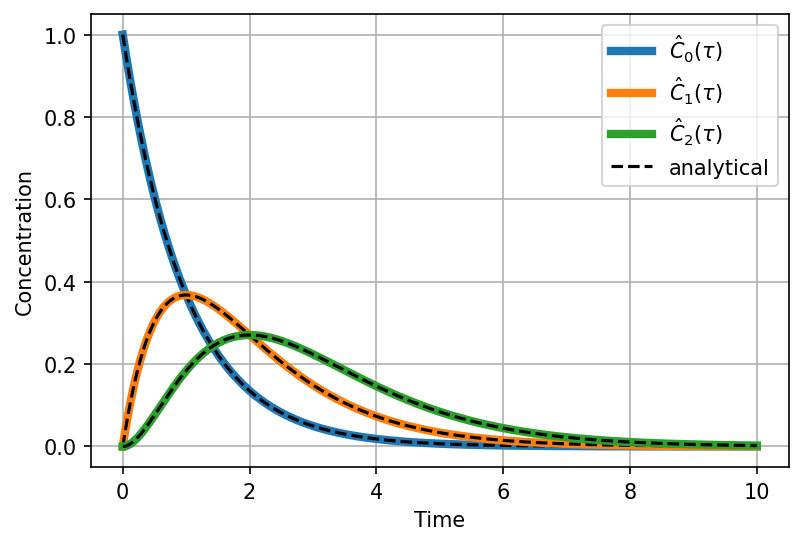
\includegraphics[width=0.9\linewidth]{fig-ode/rk4_2.png}}
  \caption{
  The concentration in the tanks. \label{fig:ode:rk4_2}
  }
\end{figure}
%\clearpage % flush figures fig:ode:rk4_2

% % endif

\section{Stiff sets of ODE  and implicit methods}
\index{stiff equations}
\index{implicit method}
As already mentioned a couple of times, our system could be part of a much larger system. To illustrate this, let us now assume that we have two 
tanks in series. The first tank is similar to our original tank, but the second tank is a sampling tank, 1000 times smaller.   

\begin{figure}[!ht]  % fig:ode:cstr2
  \centerline{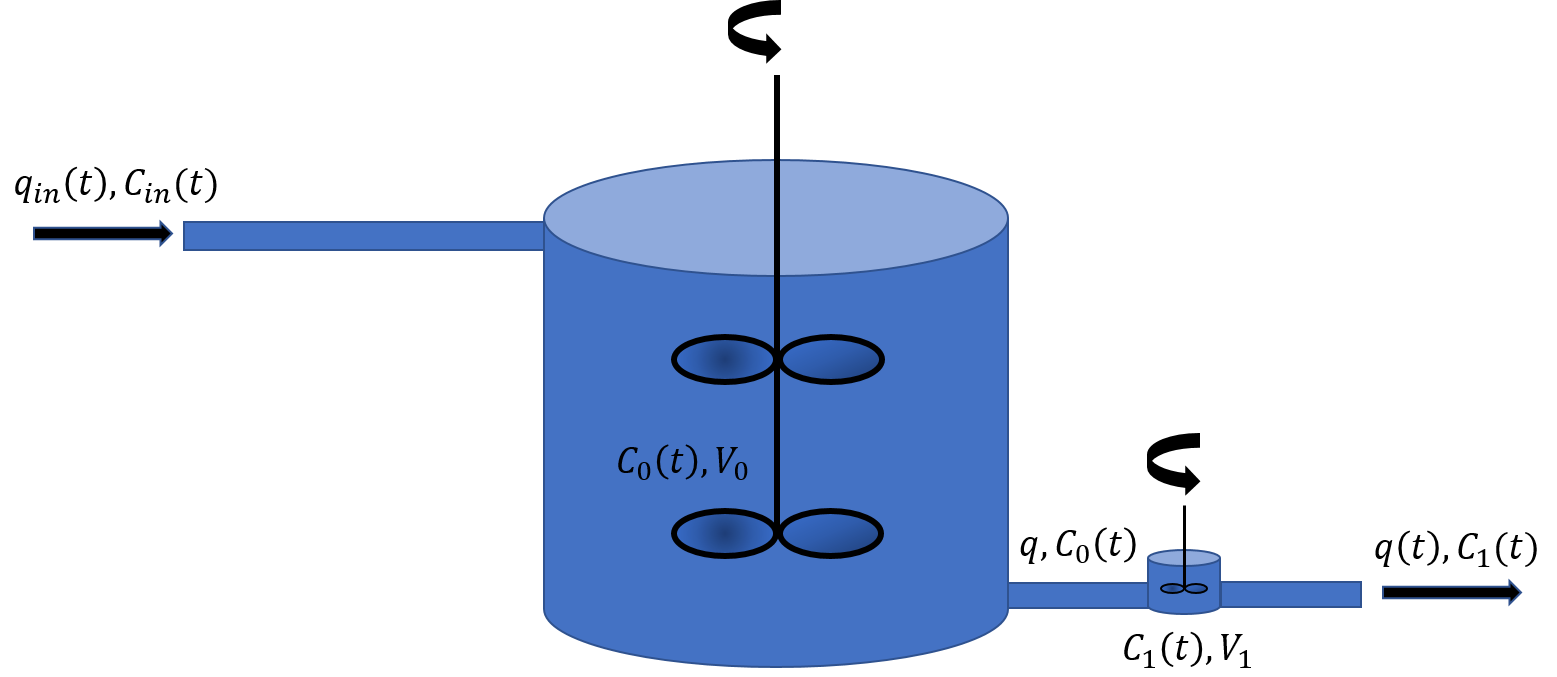
\includegraphics[width=0.9\linewidth]{fig-ode/cstr2.png}}
  \caption{
  A continuous stirred tank model with a sampling vessel. \label{fig:ode:cstr2}
  }
\end{figure}
%\clearpage % flush figures fig:ode:cstr2

The governing equations can be found by requiring mass balance for each of the tanks (see equation (\ref{eq:ode:mbal}):
\begin{align}
C_0(t+\Delta t)\cdot V_0 - C_0(t)\cdot V_0 &= q(t)\cdot C_\text{in}(t)\cdot \Delta t - q(t)\cdot C_0(t)\cdot \Delta t.\nonumber\\ 
C_1(t+\Delta t)\cdot V_1 - C_1(t)\cdot V_1 &= q(t)\cdot C_0(t)\cdot \Delta t - q(t)\cdot C_1(t)\cdot \Delta t.
\label{eq:ode:cstr2a}
\end{align}
Taking the limit $\Delta t\to 0$, we can write equation (\ref{eq:ode:cstr2a}) as:
\begin{align}
V_0\frac{dC_0(t)}{dt} &= q(t)\left[C_\text{in}(t) - C_0(t)\right].\label{eq:ode:cstr2bb}\\ 
V_1\frac{dC_1(t)}{dt} &= q(t)\left[C_0(t) - C_1(t)\right].\label{eq:ode:cstr2b}
\end{align}
Assume that the first tank is filled with seawater, $C_0(0)=C_{0,0}$, and fresh water is flooded into the tank, i.e.~$C_\text{in}=0$. Before we start to consider a numerical
solution, let us first find the analytical solution: As before the solution for the first tank (equation (\ref{eq:ode:cstr2bb})) is:
\begin{equation}
C_0(t)=C_{0,0}e^{-t/\tau_0},
\end{equation}
where $\tau_0\equiv V_0/q$. Inserting this equation into equation (\ref{eq:ode:cstr2b}), we get:
\begin{align}
\frac{dC_1(t)}{dt} &= \frac{1}{\tau_1}\left[C_{0,0}e^{-t/\tau_0} - C_1(t)\right],\nonumber\\ 
\frac{d}{dt}\left[e^{t/\tau_2}C_1\right]&= \frac{C_{0,0}}{\tau_1}e^{-t(1/\tau_0-1/\tau_1)}\label{eq:ode:cstr2c},\\ 
C_1(t)&=\frac{C_{0,0}}{1-\frac{\tau_1}{\tau_0}}\left[e^{-t/\tau_0}-e^{-t/\tau_1}\right],\label{eq:ode:cstr2d}
\end{align}
where $\tau_1\equiv V_1/q$.

Next, we will consider the numerical solution. You might think that these equations are more simple to solve numerically than the equations with three tanks
in series discussed in the previous section. Actually, this system is much harder to solve with the methods we have discussed so far.
The reason is that there are now \emph{two time scales} in the system, $\tau_1$ and $\tau_2$. The smaller tank sets a strong limitation on the step size
we can use, because we should never use step sizes larger than a tank volume. Thus if you use the code in the previous section to solve equation
(\ref{eq:ode:cstr2bb}) and (\ref{eq:ode:cstr2b}), it will not find the correct solution, unless the step size is lower than $10^{-3}$. Equations of this type
are known as \emph{stiff}. 


\begin{graybox2admon}[Stiff equations]
There is no precise definition of ''stiff'', but it is used to describe a system of differential equations, where the numerical solution becomes unstable unless
a very small step size is chosen. Such systems occurs because there are several (length, time) scales in the system, and the numerical solution is constrained
by the shortest length scale. You should always be careful on how you scale your variables in order to make the system dimensionless, which is of 
particular importance when you use adaptive methods.
\end{graybox2admon}




These types of equations are often encountered in practical applications. If our sampling tank was extremely small, maybe $10^6$ smaller than the chemical
reactor, then we would need a step size of the order of $10^{-8}$ or lower to solve the system. This step size is so low that we easily run into trouble
with round off errors in the computer. In addition the simulation time is extremely long.  How do we deal with this problem? The solution is actually
quite simple. The reason we run into trouble is that we require that the concentration leaving the tank must be a small perturbation of the old one.
This is not necessary, and it is best illustrated with Eulers method. As explained earlier Eulers method can be viewed as a two step process:
first we inject a volume (and remove an equal amount: $qC(t)\Delta t$), and then we mix. Clearly when we try to remove more than what is left, we run into
trouble. What we want to do is to remove or flood much more than one tank volume through the tank during one time step, this can be achieved by
$q(t)C(t)\Delta t\to q(t+\Delta t)C(t+\Delta t)\Delta t$. The term $q(t+\Delta t)C(t+\Delta t)\Delta t$ now represents
\emph{the mass out of the system during the time step $\Delta t$}.

The methods we have considered so far are known as \emph{explicit}, whenever we replace the solution in the right hand side of our algorithm with $y(t+\Delta t)$
or ($y_{n+1}$),
the method is known as \emph{implicit}. Implicit methods are always stable, meaning that we can take as large a time step that we would like, without
getting oscillating solution. It does not mean that we will get a more accurate solution, actually explicit methods are usually more accurate.



\begin{graybox2admon}[Explicit and Implicit methods]
Explicit methods are often called \emph{forward} methods, as they use only information from the previous step to estimate the next value. The explicit
methods are easy to implement, but get into trouble if the step size is too large. Implicit methods are often called \emph{backward} methods as the next 
step cannot be calculated directly from the previous solution, usually a non-linear equation has to be solved. Implicit methods are generally much
more stable, but the price is often lower accuracy. Many commercial simulators uses implicit methods extensively because they are stable, and stability is often viewed
as a much more important criterion than numerical accuracy.
\end{graybox2admon}



Let us consider our example further, and for simplicity use the implicit Eulers method:
\begin{align}
{C_0}_{n+1}V_0 - {C_0}_nV_0 &= q(t+\Delta t){C_\text{in}}_{n+1}\Delta t -
q(t+\Delta t){C_0}_{n+1}\Delta t.\nonumber\\ 
{C_1}_{n+1}V_1 - {C_1}_nV_1 &= q(t+\Delta t){C_0}_{n+1}\Delta t - q(t+\Delta t){C_1}_{n+1}\Delta t.
\label{eq:ode:cstr2ai}
\end{align}
This equation is equal to equation (\ref{eq:ode:cstr2a}), but the concentrations on the right hand side are now evaluated at the next time step.
The immediate problem is now that we have to find an expression for $C_{n+1}$ that is given in terms of known variables. In most cases one needs
to use a root finding method, like Newtons method, in order to solve equation (\ref{eq:ode:cstr2ai}). In this case it is straight forward to show:
\begin{align}
{C_0}_{n+1}&=\frac{{C_0}_n + \frac{\Delta t}{\tau_0}{C_\text{in}}_{n+1}}{1+\frac{\Delta t}{\tau_0}},\nonumber\\ 
{C_2}_{n+1}&=\frac{{C_1}_n + \frac{\Delta t}{\tau_1}{C_0}_{n+1}}{1+\frac{\Delta t}{\tau_1}}.\label{eq:ode:cstri1}
\end{align}
In figure~\ref{fig:ode:euler_imp} the result of the implementation is shown, note that quite large step sizes can be used without inducing non physical results.
% Below is an implementation
% % if FORMAT == 'ipynb':
% Run the script below and inspect the results.
% @@@CODE src-ode/euler_imp_2.py
% % endif
% % if FORMAT != 'ipynb':
% @@@CODE src-ode/euler_imp_2.py  fromto: def fm@# rest

\begin{figure}[!ht]  % fig:ode:euler_imp
  \centerline{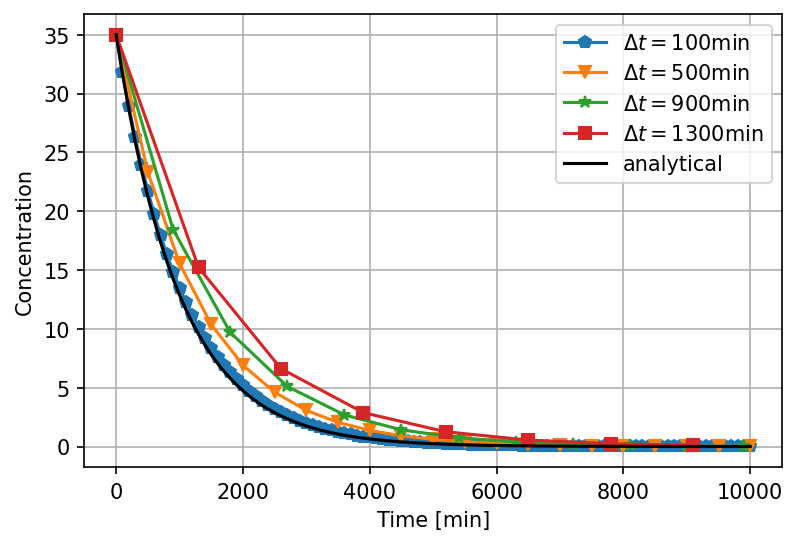
\includegraphics[width=0.9\linewidth]{fig-ode/euler_imp.png}}
  \caption{
  The concentration in the tanks for $h=0.01$.\label{fig:ode:euler_imp}
  }
\end{figure}
%\clearpage % flush figures fig:ode:euler_imp

% % endif

% --- begin exercise ---
\begin{doconceexercise}
\refstepcounter{doconceexercisecounter}

\exercisesection{Exercise \thedoconceexercisecounter: Truncation error in Euler's method}
                             

In the following we will take a closer look at the adaptive Eulers algorithm and show that the 
constant $c$ is indeed the same in equation (\ref{eq:ode:aeb0}) and (\ref{eq:ode:aeb1}). 
The true solution $y(t)$, obeys the following equation:
\begin{align}
\frac{dy}{dt}&=f(y,t),\label{eq:ode:ay}
\end{align}
and Eulers method to get from $y_0$ to $y_1$ by taking one (large) step, $h$ is:
\begin{align}
y^*_1&=y_0+hf(y_0,t_0),\label{eq:ode:ae0}
\end{align}
We will also assume (for simplicity) that in our starting point $t=t_0$, the numerical solution, $y_0$, is equal to the true solution, $y(t_0)$, hence $y(t_0)=y_0$.

% --- begin solution of exercise ---
\paragraph{Solution.}
The local error, is the difference between the numerical solution and the true solution:
\begin{align}
\epsilon^*&=y(t_0+h)-y_{1}^*=y(t_0)+y^{\prime}(t_0)h+\frac{1}{2}y^{\prime\prime}(t_0)h^2+\mathcal{O}(h^3)\nonumber\\ 
&-\left[y_0+hf(y_0,t_0+h)\right],
\end{align}
where we have used Taylor expansion to expand the true solution around $t_0$, and equation (\ref{eq:ode:ae0}).
Using equation (\ref{eq:ode:ay}) to replace $y^\prime(t_0)$ with $f(y_0,t_0)$, we find:
\begin{align}
\epsilon^*=&y(t_0+h)-y_{1}^*=\frac{1}{2}y^{\prime\prime}(t_0)h^2\equiv ch^2,
\end{align}
where we have ignored terms of higher order than $h^2$, and defined $c$ as $c=y^{\prime\prime}(t_0)/2$. Next we take two steps of size $h/2$ to
reach $y_1$:  
\begin{align}
y_{1/2}&=y_0+\frac{h}{2}f(y_0,t_0),\label{eq:ode:ae1}\\ 
y_{1}&=y_{1/2}+\frac{h}{2}f(y_{1/2},t_0+h/2),\label{eq:ode:ae2}\\ 
y_{1}&=y_{0}+\frac{h}{2}f(y_0,t_0)+\frac{h}{2}f(y_0+\frac{h}{2}f(y_0,t_0),t_0+h/2).\label{eq:ode:ae3}
\end{align}
Note that we have inserted
equation (\ref{eq:ode:ae1}) into equation (\ref{eq:ode:ae2}) to arrive at equation (\ref{eq:ode:ae3}). The truncation error in this case is, as before:
\begin{align}
\epsilon&=y(t_0+h)-y_{1}=y(t_0)+y^{\prime}(t_0)h+\frac{1}{2}y^{\prime\prime}(t_0)h^2+\mathcal{O}(h^3)\nonumber\\ 
&-\left[y_{0}+\frac{h}{2}f(y_0,t_0)+\frac{h}{2}f(y_0+\frac{h}{2}f(y_0,t_0),t_0+h/2)\right].\label{eq:ode:ay5}
\end{align}
This equation is slightly more complicated, due to the term involving $f$ inside the last parenthesis, we can use Taylor expansion to expand it about $(y_0,t_0)$:
\begin{align}
&f(y_0+\frac{h}{2}f(y_0,t_0),t_0+h/2)=f(y_0,t_0)\nonumber\\ 
&+\frac{h}{2}\left[f(y_0,t_0)\left.\frac{\partial f}{\partial y}\right|_{y=y_0,t=t_0}
+\left.\frac{\partial f}{\partial t}\right|_{y=y_0,t=t_0}\right]+\mathcal{O}(h^2).\label{eq:ode:ay2}
\end{align}
It turns out that this equation is related to $y^{\prime\prime}(t_0,y_0)$, which can be seen by differentiating equation (\ref{eq:ode:ay}):
\begin{align}
\frac{d^2y}{dt^2}&=\frac{df(y,t)}{dt}=\frac{\partial f(y,t)}{\partial y}\frac{dy}{dt}+\frac{\partial f(y,t)}{\partial t}
=\frac{\partial f(y,t)}{\partial y}f(y,t)+\frac{\partial f(y,t)}{\partial t}.\label{eq:ode:ay3}
\end{align}
Hence, equation (\ref{eq:ode:ay2}) can be written:
\begin{align}
f(y_0+\frac{h}{2}f(y_0,t_0),t_0+h/2)=f(y_0,t_0)+\frac{h}{2}y^{\prime\prime}(t_0,y_0),\label{eq:ode:ay4}
\end{align}
hence the truncation error in equation (\ref{eq:ode:ay5}) can finally be written:
\begin{align}
\epsilon=&y(t_1)-y_{1}=\frac{h^2}{4} y^{\prime\prime}(y_0,t_0)=\frac{1}{2}ch^2,\label{eq:ode:ae4}
\end{align}

% --- end solution of exercise ---

% --- begin subexercise ---

\subex{a)}
Show that when we take one step of size $h$ from $t_0$ to $t_1=t_0+h$, $c=y^{\prime\prime}(t_0)/2$ in equation (\ref{eq:ode:aeb0}).

% --- begin answer of exercise ---
\paragraph{Answer.}
The local error, is the difference between the numerical solution and the true solution:
\begin{align}
\epsilon^*&=y(t_0+h)-y_{1}^*=y(t_0)+y^{\prime}(t_0)h+\frac{1}{2}y^{\prime\prime}(t_0)h^2+\mathcal{O}(h^3)\nonumber\\ 
&-\left[y_0+hf(y_0,t_0+h)\right],
\end{align}
where we have used Taylor expansion to expand the true solution around $t_0$, and equation (\ref{eq:ode:ae0}).
Using equation (\ref{eq:ode:ay}) to replace $y^\prime(t_0)$ with $f(y_0,t_0)$, we find:
\begin{align}
\epsilon^*=&y(t_0+h)-y_{1}^*=\frac{1}{2}y^{\prime\prime}(t_0)h^2\equiv ch^2,
\end{align}
hence $c=y^{\prime\prime}(t_0)/2$.
% --- end answer of exercise ---

% --- end subexercise ---

% --- begin subexercise ---

\subex{b)}
Show that when we take two steps of size $h/2$ from $t_0$ to $t_1=t_0+h$, Eulers algorithm is:
\begin{align}
y_{1}&=y_{0}+\frac{h}{2}f(y_0,t_0)+\frac{h}{2}f(y_0+\frac{h}{2}f(y_0,t_0),t_0+h/2).
\end{align}

% --- begin answer of exercise ---
\paragraph{Answer.}
\begin{align}
y_{1/2}&=y_0+\frac{h}{2}f(y_0,t_0),\label{eq:ode:ae1b}\\ 
y_{1}&=y_{1/2}+\frac{h}{2}f(y_{1/2},t_0+h/2),\label{eq:ode:ae2b}\\ 
y_{1}&=y_{0}+\frac{h}{2}f(y_0,t_0)+\frac{h}{2}f(y_0+\frac{h}{2}f(y_0,t_0),t_0+h/2).\label{eq:ode:ae3b}
\end{align}
Note that we have inserted
equation (\ref{eq:ode:ae1b}) into equation (\ref{eq:ode:ae2b}) to arrive at equation (\ref{eq:ode:ae3b}).
% --- end answer of exercise ---

% --- end subexercise ---

% --- begin subexercise ---

\subex{c)}
Find an expression for the local error when using two steps of size $h/2$, and show that the local error is: $\frac{1}{2}ch^2$

% --- begin answer of exercise ---
\paragraph{Answer.}
\begin{align}
\epsilon&=y(t_0+h)-y_{1}=y(t_0)+y^{\prime}(t_0)h+\frac{1}{2}y^{\prime\prime}(t_0)h^2+\mathcal{O}(h^3)\nonumber\\ 
&-\left[y_{0}+\frac{h}{2}f(y_0,t_0)+\frac{h}{2}f(y_0+\frac{h}{2}f(y_0,t_0),t_0+h/2)\right].\label{eq:ode:ay5b}
\end{align}
This equation is slightly more complicated, due to the term involving $f$ inside the last parenthesis, we can use Taylor expansion to expand it about $(y_0,t_0)$:
\begin{align}
&f(y_0+\frac{h}{2}f(y_0,t_0),t_0+h/2)=f(y_0,t_0)\nonumber\\ 
&+\frac{h}{2}\left[f(y_0,t_0)\left.\frac{\partial f}{\partial y}\right|_{y=y_0,t=t_0}
+\frac{h}{2}\left.\frac{\partial f}{\partial t}\right|_{y=y_0,t=t_0}\right]+\mathcal{O}(h^2).\label{eq:ode:ay2b}
\end{align}
It turns out that this equation is related to $y^{\prime\prime}(t_0,y_0)$, which can be seen by differentiating equation (\ref{eq:ode:ay}):
\begin{align}
\frac{d^2y}{dt^2}&=\frac{df(y,t)}{dt}=\frac{\partial f(y,t)}{\partial y}\frac{dy}{dt}+\frac{\partial f(y,t)}{\partial t}
=\frac{\partial f(y,t)}{\partial y}f(y,t)+\frac{\partial f(y,t)}{\partial t}.\label{eq:ode:ay3b}
\end{align}
Hence, equation (\ref{eq:ode:ay2b}) can be written:
\begin{align}
f(y_0+\frac{h}{2}f(y_0,t_0),t_0+h/2)=f(y_0,t_0)+\frac{h}{2}y^{\prime\prime}(t_0,y_0),\label{eq:ode:ay4b}
\end{align}
hence the truncation error in equation (\ref{eq:ode:ay5b}) can finally be written:
\begin{align}
\epsilon=&y(t_1)-y_{1}=\frac{h^2}{4} y^{\prime\prime}(y_0,t_0)=\frac{1}{2}ch^2,\label{eq:ode:ae4b}
\end{align}
% --- end answer of exercise ---

% --- end subexercise ---

\end{doconceexercise}
% --- end exercise ---

% !split
\chapter{Monte Carlo Methods}
\label{ch:mc}

\section{Monte Carlo methods}
Monte Carlo methods are named after the Monte Carlo Casino in Monaco,
this is because at its core it uses random numbers to solve problems.
Monte Carlo methods are quite easy to program, and they are
usually much more intuitive than a theoretical approach. 
% If we would
% like to find the probability to get at least 5 on three dices after 5 throws
% there are methods from statistics that could tell us the probability.
% Using the Monte Carlo method, we would get the computer to pick a
% random integer between 1 and 6, three times, to represent one throw of
% the dices bla bla.
% later in this chapter
% Usually  Usually we use differential equations to describe physical systems, the solution to these equations are continuous functions. In order for these solutions
% to be useful, they require that the differential equation describes our physical sufficiently. In many practical cases we have no control over many

% of the parameters entering the differential equation, or stated differently \emph{our system is not deterministic}. This means that there could be some random
% fluctuations, occurring at different times and points in space, that we have no control over. In a practical situation we might would like to investigate how these fluctuations would
% affect the behavior of our system. A

% o \href{{https://www.scratchapixel.com/lessons/mathematics-physics-for-computer-graphics/monte-carlo-methods-in-practice/monte-carlo-rendering-practical-example}}{ray  tracing}\footnote{\texttt{https://www.scratchapixel.com/lessons/mathematics-physics-for-computer-graphics/monte-carlo-methods-in-practice/monte-carlo-rendering-practical-example}}

\section{Monte Carlo integration  ''hit and miss''}
\index{Monte Carlo integration}
Let us start with a simple illustration of the Monte Carlo Method (MCM), Monte Carlo integration. To the left
in figure~\ref{fig:mc:mci} there is a shape of a pond. Imagine that we wanted to estimate the area of the pond, how could
we do it? Assume further that you did not have your phone or any other electronic devices to help you. 

\begin{figure}[!ht]  % fig:mc:mci
  \centerline{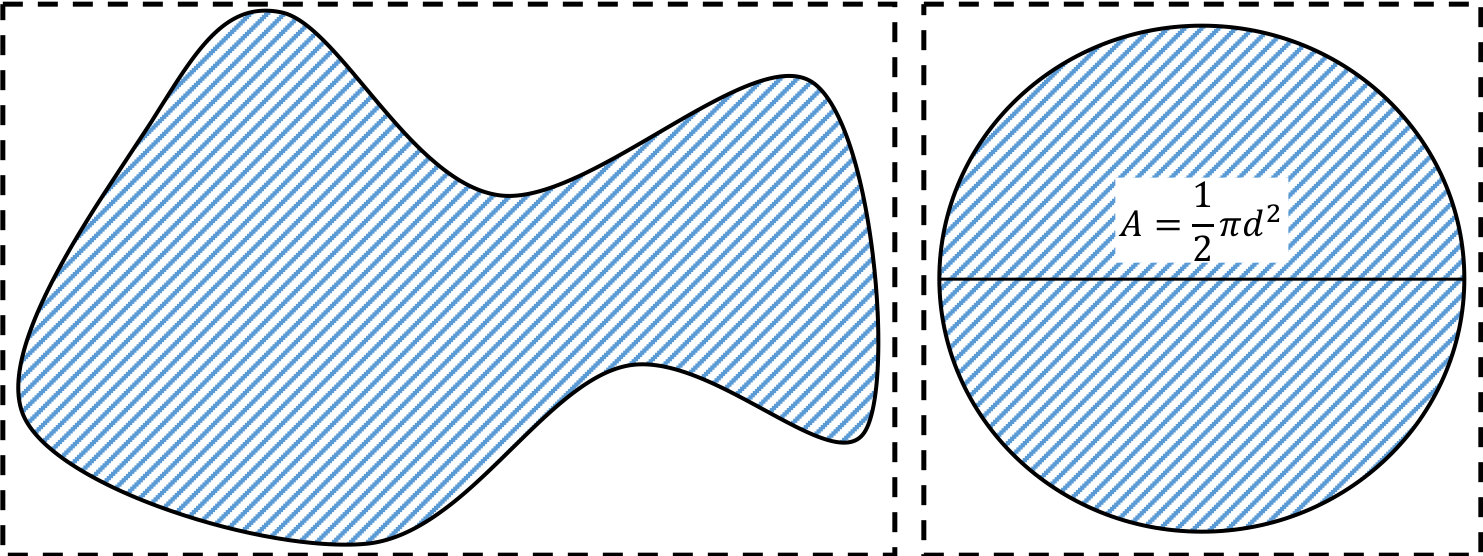
\includegraphics[width=1.0\linewidth]{fig-mc/mci.png}}
  \caption{
  Two ponds to illustrate the MCM. \label{fig:mc:mci}
  }
\end{figure}
%\clearpage % flush figures fig:mc:mci

One possible approach is: First to walk around it, and put up some bands (illustrated by the black dotted line).
Then estimate the area inside the bands (e.g.~4$\times$3 meters). Then
we would know that the area was less than e.g.~12m$^2$. Finally,
and this is the difficult part, throw rocks \emph{randomly} inside the
bands. The number of rocks hitting the pond divided by the total
number rocks thrown should be equal to the area of the pond divided by
the total area inside the bands, i.e.~the area of the pond should be
equal to:
\begin{equation}
A\simeq\text{Area of rectangle}\times\frac{\text{Number of rocks hitting the pond}}{\text{Number of rocks thrown}}.
\label{eq:mc:mci}
\end{equation}
It is important that we throw the rocks randomly, otherwise  equation (\ref{eq:mc:mci}) is not correct. Now, let us
investigate this in more detail, and use the idea of throwing rocks to estimate $\pi$. To the right in figure~\ref{fig:mc:mci},
there is a well known shape, a circle. The area of the circle is $\pi d^2/4$, and the shape is given by $x^2+y^2=d^2/4$. Assume that
the circle is inscribed in a square with sides of $d$. To throw rocks randomly inside the square, is equivalent pick random numbers
with coordinates $(x,y)$, where $x\in[0,d]$ and $y\in[0,d]$. We want all the $x-$ and $y-$values to be chosen with equal probability,
which is equivalent to pick random numbers from a \emph{uniform} distribution. Below is a Python implementation:


















\begin{lstlisting}[language=python,style=blue1]
import numpy as np

def estimate_pi(N,d):
#   random.seed(2)
    D2=d*d/4; dc=0.5*d
    A=0
    for k in range(0,N):
        x=np.random.uniform(0,d)
        y=np.random.uniform(0,d)
        if((x-dc)**2+(y-dc)**2 <= D2):
            A+=1
    # estimate area of circle: d*d*A/N
    return 4*A/N

N=1000;d=2
pi_est=estimate_pi(N,d)
print('Estimate for pi= ', pi_est,' Error=', np.pi-pi_est)

\end{lstlisting}


In the table below, we have run the code for $d=1$ and different values of $N$. 



{\small   % for Springer style: small table font and more vspace

\vspace{4mm}

\begin{tabular}{cccc}
\hline
\multicolumn{1}{c}{ MC estimate } & \multicolumn{1}{c}{ Error } & \multicolumn{1}{c}{ $N$ } & \multicolumn{1}{c}{ $1/\sqrt{N}$ } \\
\hline
3.04        & -0.10159    & 10$^2$ & 0.100        \\
3.176       & $\,$0.03441 & 10$^3$ & 0.032        \\
3.1584      & $\,$0.01681 & 10$^4$ & 0.010        \\
3.14072     & -0.00087    & 10$^5$ & 0.003        \\
\hline
\end{tabular}

\vspace{4mm}

}


\noindent
We clearly see that a fair amount of rocks or numbers needs to be used in order to get a good estimate. If you run this code several
times you will see that the results changes from time to time. This
makes sense as the coordinates $x$ and $y$ are chosen at random.



\begin{graybox2admon}[A note on performance]
The code above is not efficient and for MC simulations we usually have to use many random numbers. Instead of




\begin{lstlisting}[language=python,style=blue1bar]
for k in range(0,N):
        x=np.random.uniform(0,d)
        y=np.random.uniform(0,d)

\end{lstlisting}

one should avoid loops, and take advantage of build in functions in Numpy



\begin{lstlisting}[language=python,style=blue1bar]
x=np.random.uniform(0,d,size=N)
y=np.random.uniform(0,d,size=N)

\end{lstlisting}
\end{graybox2admon}



\subsection{Random number generators}
\index{random number generators}
\index{Mersenne Twister}
There are much to be said about random number generators. The MCM depends on a good random number generator, otherwise we cannot use the results from
statistics to develop our algorithms. Below, we briefly summarize some important points that you should be aware of:

\begin{enumerate}
\item Random number generators are generally of two types: \emph{hardware random number generator} (HRNG) or \emph{pseudo random number generator} (PRNG).

\item HRNG uses a physical process to generate random numbers, this could atmospheric noise, radioactive decay, microscopic fluctuations, which is translated to an electrical signal. The electrical signal is converted to a digital number (1 or 0), by sampling the random signal random numbers can be generated. The HRNG are often named \emph{true random number generators}, and their main use are in \emph{cryptography}.

\item PRNG uses a mathematical algorithm to generate an (apparent) random sequence. The algorithm uses an initial number, or a \emph{seed},  to start the sequence of random number. The sequence is deterministic, and it will generate the same sequence of numbers if the same seed is used. At some point the algorithm will reproduce itself, i.e.~it will have certain period. For some seeds the period may be much shorter.

\item Many of the PRNG are not considered to be cryptographically secure, because if a sufficiently long sequence of random numbers are generated from them, the rest of the sequence can be predicted. 

\item Python uses the \href{{https://en.wikipedia.org/wiki/Mersenne_Twister}}{Mersenne Twister}\footnote{\texttt{https://en.wikipedia.org/wiki/Mersenne\_Twister}} algorithm to generate random numbers, and has a period of $2^{19937}−1\simeq4.3\cdot10^{6001}$. It is not considered to be cryptographically secure.
\end{enumerate}

\noindent
In Pythons \texttt{random.uniform} function, a random seed is chosen each time the code is run, but
if we set e.g. \texttt{random.seed(2)}, the code will generate the same sequence of numbers each time it is called. 

\subsection{Encryption}
\index{encryption}
This section can be skipped as it is not relevant for development of
the numerical algorithms, but it is a good place to explain the basic
idea behind encryption of messages. A very simple, but not a very good
encryption, is to replace all the letters in the alphabet with a
number, e.g.~A=1, B=2, C=3, etc. This is what is know as a
\emph{substitution cipher}, it does not need to be a number it could be a
letter, a sequence of letters, letters and numbers etc. The receiver
can solve the code by doing the reverse operation.

The
weakness of this approach is that it can fairly easily be cracked, by
the following approach: First we analyze the encrypted message and find the frequency of each of the symbols.
Assume that we know that the message is written in English, then the
frequency of symbols can be compared with the frequency of
letters from a known English text (the most common is \texttt{E} (12$\%$), then \texttt{T}
(9$\%$), etc.). We would then guess that the most occurring symbol
probably is an \texttt{E} or \texttt{T}. When some of the letters are in place, we
can compare with the frequency of words, and so on. By the help of
computers this process can easily be automated.

A much better algorithm is \emph{to not replace a letter with the same
symbol}. To make it more clear, consider our simple example where A=1, B=2,
C=3, $\ldots$. If we know say that A=1 but we add a \emph{random number},
then our code would be much harder to crack. Then the letter A
could be several places in the message but represented as a complete different
number. Thus we could not use the frequency of the various symbols to
crack the message.

How can the receiver decrypt the message? Obviously, it can be done if
both the sender and receiver have the same sequence of random numbers (or the \emph{key}).
This can be achieved quite simple with random number generators, if we
know the seed  used we can generate the same sequence of
random numbers. If Alice where to send a message to Bob without Eve
knowing what it is, Alice and Bob could agree to send a message that
was scrambled using Pythons Mersenne-Twister algorithm with seed=2.

The weakness of this approach is of course that Eve could convince
Alice or Bob to give her the seed or the key. Another possibility is
that Eve could write a program that tested
different random number generators and seeds to decipher the message.
How to avoid this?

Let us assume that Alice and Bob each had their own
hardware random generator. This generator generated random numbers that was truly
random, and the sequence could not be guessed by any outsider. Alice
do not want to share her key (sequence of random numbers) with Bob,
and Bob would not share his key with Alice. How can they send a
message without sharing the key? One possible way of doing it is as
follows: Alice write a message and encrypt it with her key, she send
the message to Bob. Bob then encrypt the message with his key, he
sends it back to Alice. Alice then decrypt the message with her key
and send it back to Bob. Now, Bob can decrypt it with his own key and
read the message. The whole process can be visualized by thinking of
the message as box with the message. Alice but her padlock on the box
(keeps her key for her self), she sends the message to Bob. Bob locks
the box with his padlock, now there are two padlocks on the box. He
sends the box back to Alice, Alice unlocks her padlock with her key,
and sends it back to Bob. The box now only has Bob's key, he can
unlock the box and read the message. The important point is that the
box was never unlocked throughout the transaction, and Alice and Bob
never had to share the key with anyone. 

\subsection{Errors on Monte Carlo integration and the binomial distribution}
\index{Monte Carlo Integration, error}
\index{binomial distribution}
How many rocks do we need to throw in order to reach a certain accuracy? To answer this question we need some results from statistics. Our problem of calculating the integral is closely related to the \emph{binomial distribution}. When we throw a rock one of two things can happen i) the rock falls into the water, or ii) it falls outside the pond. If we denote the probability that the rock falls into the pond as $p$, then the probability that it falls outside the pond, $q$, has to be $q=1-p$.
This is simply because there are no other possibilities and the sum of the two probabilities has to be one: $p+q=p+(1-p)=1$. The binomial distribution is given by:
\begin{equation}
p(k)=\frac{n!}{k!(n-k)!}p^k(1-p)^{n-k}.
\label{eq:mc:bin}
\end{equation}
$p(k)$ is the probability that an event happens $k$ times after $n$ trials. The mean, $\mu$, and the variance, $\sigma^2$, of the binomial distribution is:
\begin{align}
\mu&=\sum_{k=0}^{n-1}kp(k)=np, \label{eq:mc:binm}\\ 
\sigma^2&=\sum_{k=0}^{n-1}(k-\mu)^2p(k)=np(1-p). \label{eq:mc:bins}
\end{align}


\begin{graybox2admon}[Mean and variance]
\index{mean}
\index{variance}
The mean of a distribution is simply the \emph{sum} divided by the \emph{count},
the symbol $\mu$ or $\overline{x}$ is usually used. For $N$ observations, $x_i$,
$\mu=\sum_i x_i/N$. The mean is just an average, it could e.g.~be the sum of all the heights of
students in the class divided by the number of students. The mean
would then be the average height of all the students in the class.

The variance is calculated by taking the difference between each of
the data points and the mean, square it, and sum over all data points.
Usually the symbol $\sigma^2$ is used, $\sigma^2=\sum_i(\mu-x_i)^2/N$.
The variance measures the spread in the data. Furthermore, it squares the
distance between the mean and the individual observations, meaning
that the points lying far a way from $\mu$ contributes more to the
variance.
\end{graybox2admon}



Before we proceed, we should take a moment and look a little more into
the meaning of equation (\ref{eq:mc:bin}) to appreciate its usefulness.  A classical example of the use of the binomial formula is to toss a coin, if the coin is fair it will have an equal probability of giving us a head or tail, hence $p=1/2$. Equation (\ref{eq:mc:bin}), can answer questions like: ''What is the probability to get only heads after 4 tosses?''. Let us calculate this answer using equation (\ref{eq:mc:bin}), the number of tosses is 4, the number of success is 4 (only heads each time)
\begin{equation}
p(k=4)=\frac{4!}{4!(4-4)!}\frac{1}{2}^4(1-\frac{1}{2})^{4-4}=\frac{1}{2^4}=\frac{1}{16}.
\label{eq:mc:coin}
\end{equation}
''What is the probability to get three heads in four tosses?'', using
the same equation, we find:
\begin{equation}
p(k=3)=\frac{4!}{3!(4-3)!}\frac{1}{2}^3(1-\frac{1}{2})^{4-3}=\frac{4}{2^4}=\frac{1}{4}.
\label{eq:mc:coin2}
\end{equation}
In figure~\ref{fig:mc:coin}, all the possibilities are shown. The
number of possibilities are 16, and there are only one possibility
that we get only heads, i.e.~the probability is 1/16 as calculated in
equation (\ref{eq:mc:coin}). In the figure we also see that there are 4
possible ways we can get three heads, hence the probability is
4/16=1/4 as calculated in equation (\ref{eq:mc:coin2}).

\begin{figure}[!ht]  % fig:mc:coin
  \centerline{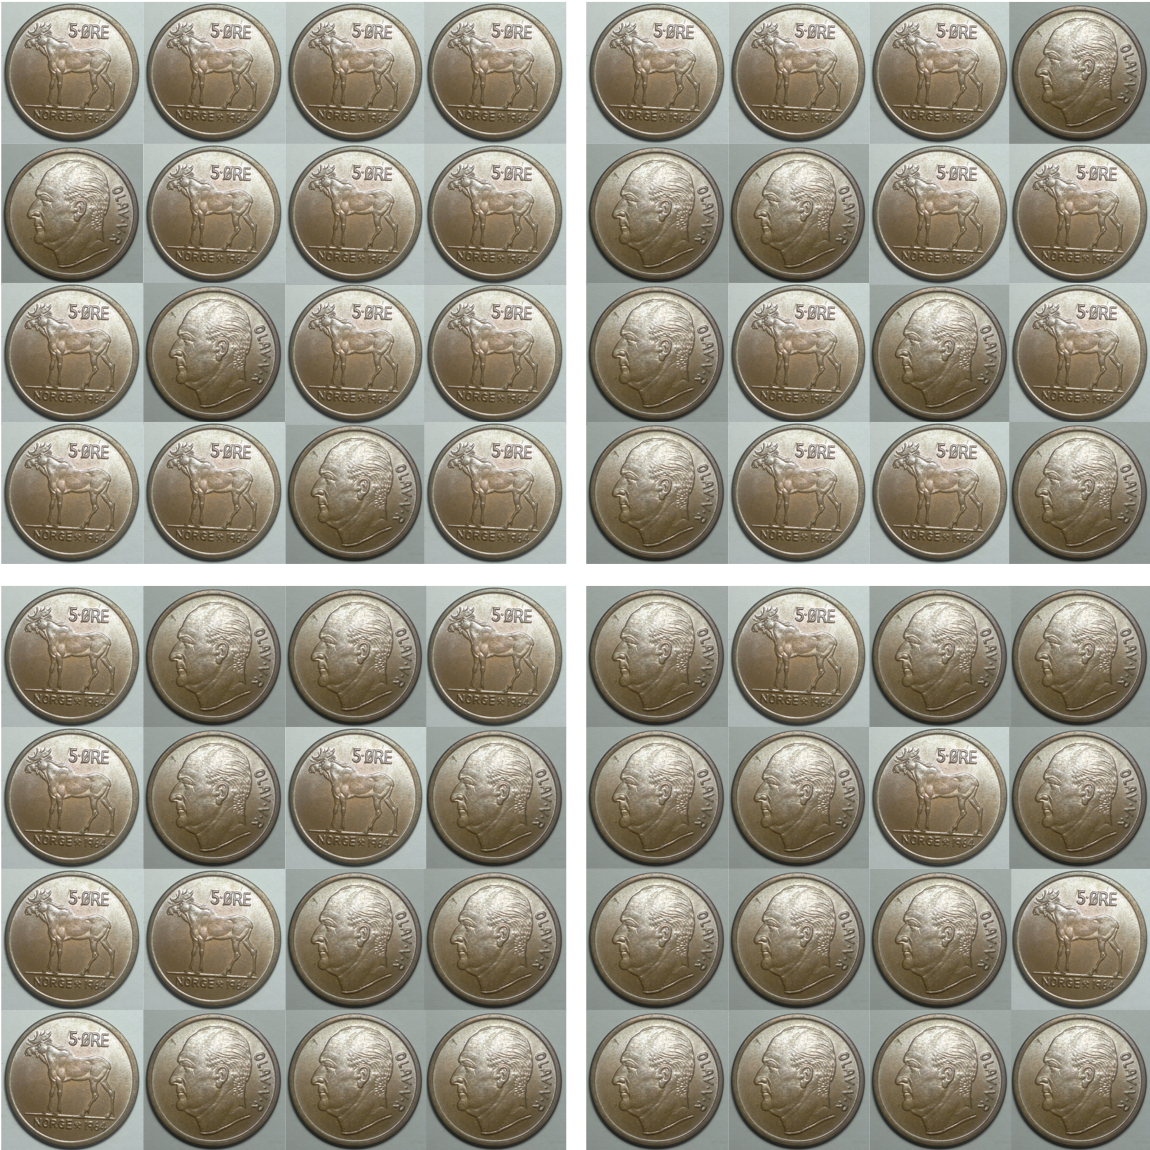
\includegraphics[width=1.0\linewidth]{fig-mc/coin.png}}
  \caption{
  The famous Norwegian Moose coin, and possible outcomes of four coin flips in a row. \label{fig:mc:coin}
  }
\end{figure}
%\clearpage % flush figures fig:mc:coin

Now, let us return to our original question, ''What is the error on our
estimate of the integral, when using the MCM?''. Before we continue we
should also clean up our notation, let $I$ be the value of the true
integral, $A$ is our \emph{estimate} of the integral, and $I_N$ is the area
of the rectangle. First, let us show
that the mean or expectation value of the binomial distribution is
related to our estimate of the area of the pond or the circle, $A$. In our case we draw $n=N$
random numbers, and $k$ times the coordinate falls inside the circle,
equation (\ref{eq:mc:binm}) tells us that the mean value is $np$. $p$
is the probability that the coordinate is within the area to be
integrated, hence as before $p$ is equal to the area to be integrated
divided by the area of the total domain, thus:
\begin{equation}
\mu=np=N\frac{A}{I_N},
\end{equation}
or
\begin{equation}
A=I_N\frac{\mu}{N}.
\end{equation}
Equation (\ref{eq:mc:bins}), gives us an estimate of the variance of
the mean value. Assume for simplicity that we can replace $1-p\simeq
p$, this is of course only correct if the area of the rectangle is
twice as big as our pond, but we are only interested in an
estimate of the error, hence $\sigma^2\simeq np^2$. We can now use the
standard deviation as an estimate of the error of our integral:
\begin{align}
I&\simeq I_N\frac{\mu\pm\sigma}{n}=I_N\frac{Np\pm \sqrt{N}p}{N}\nonumber\\ 
&\simeq I_N(p\pm \frac{p}{\sqrt{N}})=A\pm \frac{A}{\sqrt{N}}.
\label{eq:mc:mcmf}
\end{align}
In the last equation we have replaced $p$ with $A/I_N$. 
Hence, the error of our integral is inversely proportional to the
square root of the number of points. 

\subsection{The mean value method}
\index{Monte Carlo integration, mean value}
How does our previous method compare with some of our standard methods,
like the midpoint rule? The error for the MC method scales as
$1/\sqrt{N}$, in our previous error estimates we used the step length,
$h$, as an indicator of the accuracy, and not $N$. The s$N$ is
related to the number of points as $h=(b-a)/n$, where $b$ and $a$ are
the integration limit. Thus our MCM scales as $1/\sqrt{n}\sim
h^{1/2}$, this is actually worse than the midpoint or trapezoidal
rule, which scaled as $h$.

The MCM can be improved. We will first describe the mean value method.
In the last section we calculated the area of
a circle by picking random numbers inside a square and estimated the
fraction of points inside the circle. This is equivalent to calculate
the area of a half circle, and multiply with 2:
\begin{equation}
I=2\int_{-d/2}^{d/2}\sqrt{(d/2)^2-x^2}dx=\frac{\pi d^2}{4}.
\label{eq:mc:Is}
\end{equation}
The half-circle is now centered at the origin. Before we proceed we
write our integral in a general form as:
\begin{equation}
I=\int_a^bf(x)dx.
\label{eq:mc:I1}
\end{equation}
Instead of counting the number of points inside the curve given by
$f(x)$, we could instead use the mean of
the function, which we will define as $\overline{f}=\sum_k f(x_k)/N$:
\begin{equation}
I=\int_a^bf(x)dx\simeq\overline{f}\int_a^bdx=(b-a)\overline{f}
=\frac{(b-a)}{N}\sum_{k=0}^{N-1}f(x_k).
\label{eq:mc:I2}
\end{equation}
Note that this formula is similar to the midpoint rule, but now the
function is not evaluated at the midpoint, but at several points and
we use the average value. 

\begin{figure}[!ht]  % fig:mc:int
  \centerline{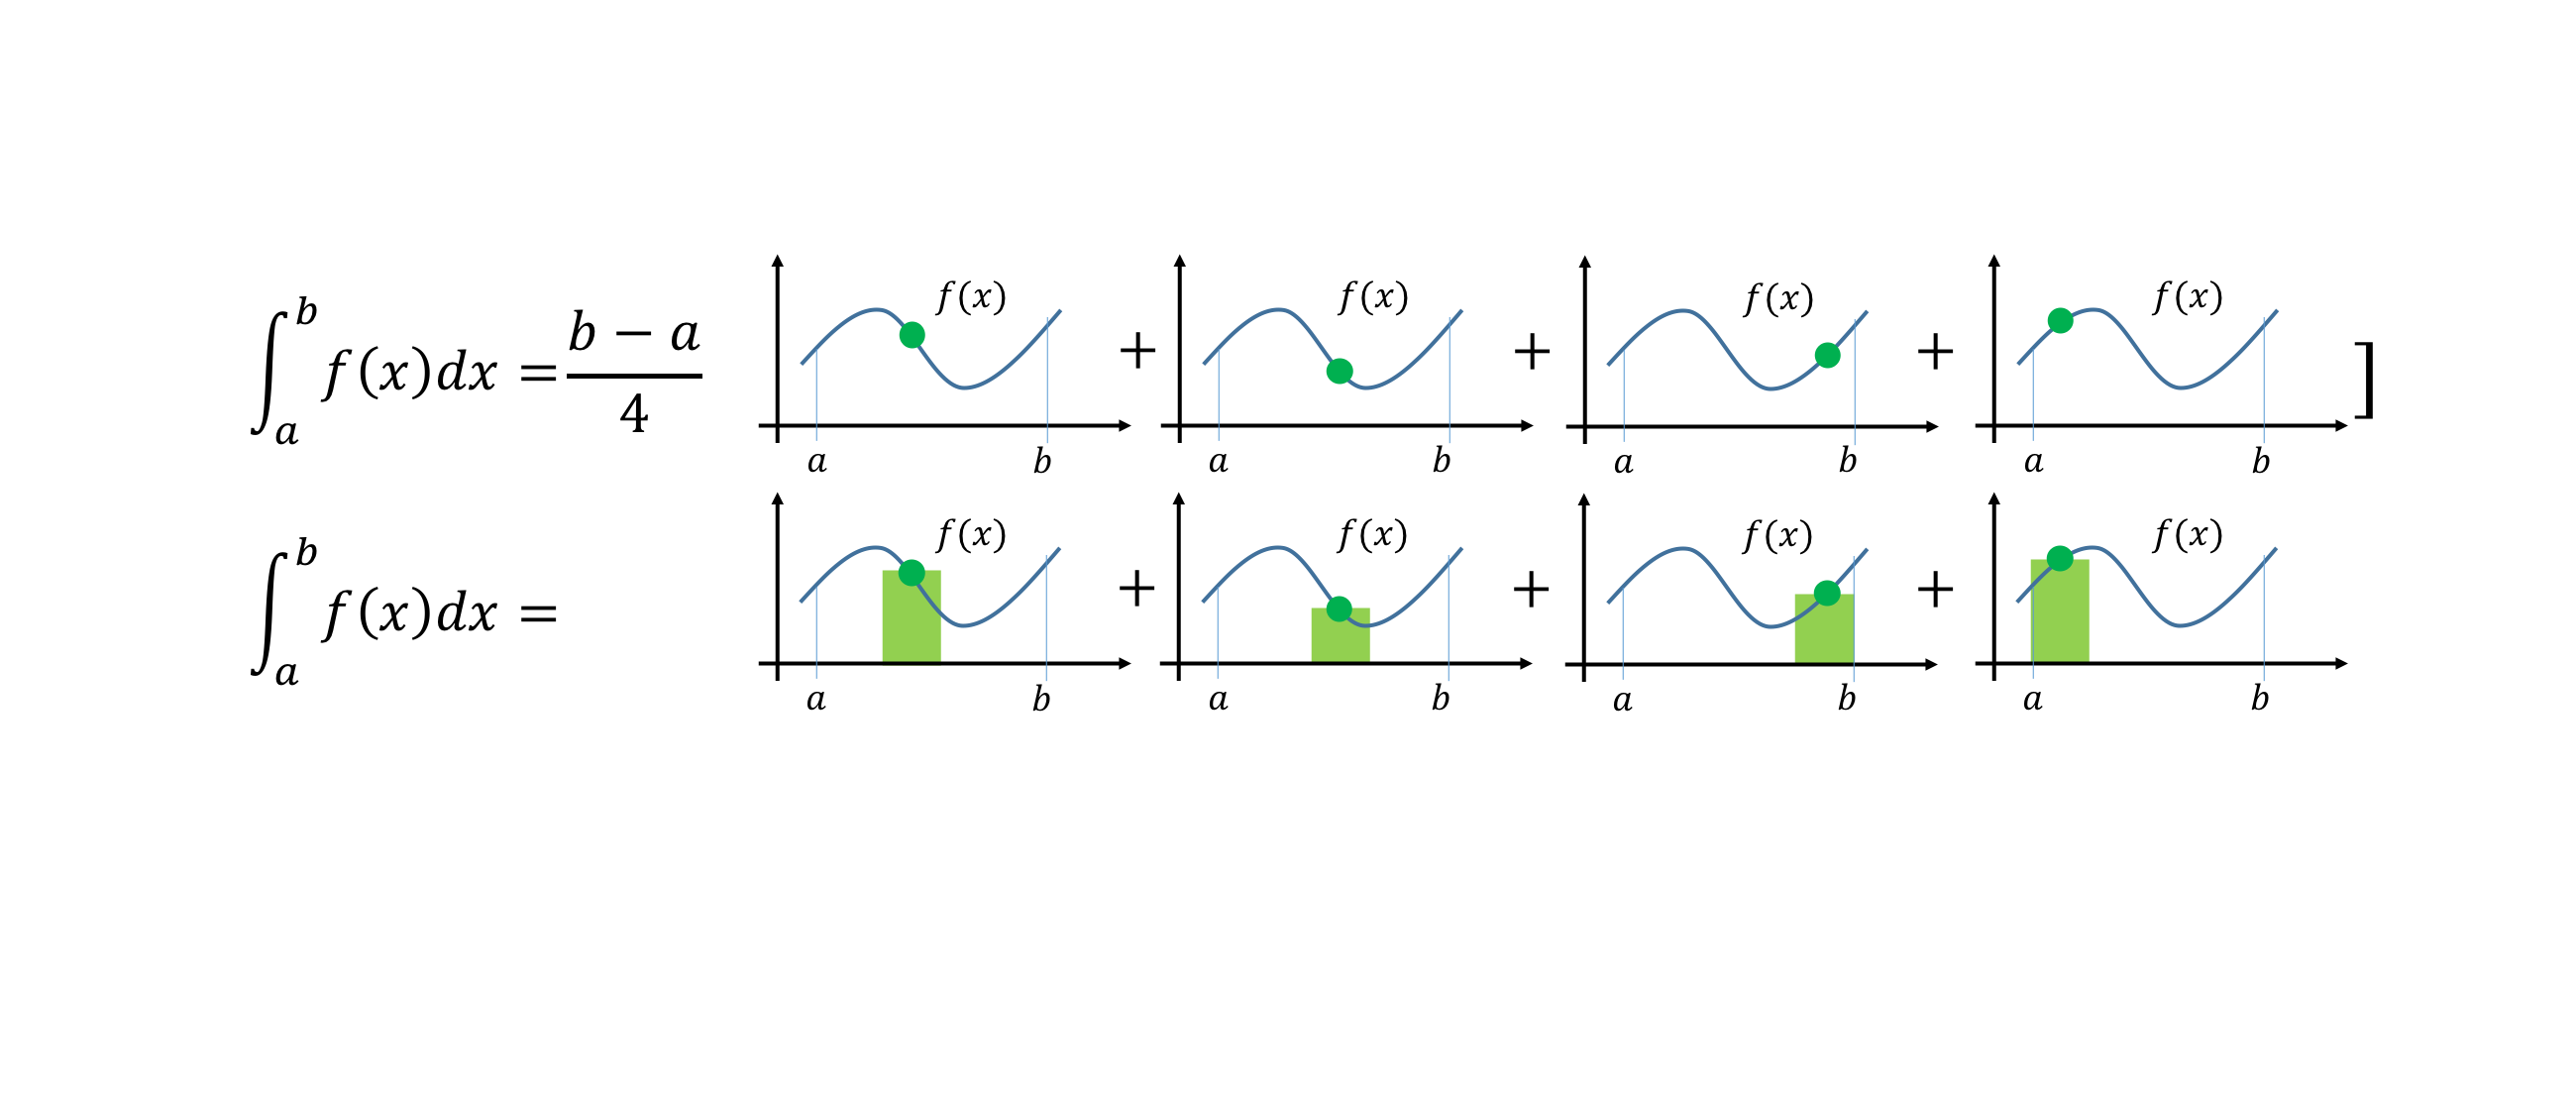
\includegraphics[width=1.0\linewidth]{fig-mc/mcint.png}}
  \caption{
  Illustration of MC integration for $N=4$. \label{fig:mc:int}
  }
\end{figure}
%\clearpage % flush figures fig:mc:int

Below is an implementation:












\begin{lstlisting}[language=python,style=blue1]
import numpy as np

def f(x,D2):
    return 2*np.sqrt((D2-x*x))

def mcm_mean(N,d):
    D2=d*d/4
    x=np.random.uniform(-d/2,d/2,size=N)
    A=np.sum(f(x,D2))
    # estimate for area: A/N
    return d*A/N

\end{lstlisting}


In the table below we have compared the mean value method with the
''hit and miss'' method. We see
that the mean value method performs somewhat better, but there are
some random fluctuations and in some cases it performs poorer. 



{\small   % for Springer style: small table font and more vspace

\vspace{4mm}

\begin{tabular}{ccccc}
\hline
\multicolumn{1}{c}{ MC-mean } & \multicolumn{1}{c}{ Error } & \multicolumn{1}{c}{ MC } & \multicolumn{1}{c}{ Error } & \multicolumn{1}{c}{ $N$ } \\
\hline
3.1706  & 0.0290  & 3.1600 & 0.0184 & 10$^2$ \\
3.1375  & -0.0041 & 3.1580 & 0.0164 & 10$^3$ \\
3.1499  & 0.0083  & 3.1422 & 0.0006 & 10$^4$ \\
3.1424  & 0.0008  & 3.1457 & 0.0041 & 10$^5$ \\
3.1414  & -0.0002 & 3.1422 & 0.0006 & 10$^6$ \\
\hline
\end{tabular}

\vspace{4mm}

}


\noindent
We also see that in this case the error scales as $1/\sqrt{N}$.


\begin{graybox2admon}[Notice]
At first sight it might be a little counter intuitive that if we
multiply the average value of the function with the size of the
integration domain we get an estimate for the integral, as illustrated
in the top figure in figure~\ref{fig:mc:int}. A different, but
equivalent way, of viewing the mean value method is the lower figure
in figure~\ref{fig:mc:int}. For each random point we choose, we
multiply with the area $(b-a)/N$, as $N$ increases the area decreases
and the mean value method approaches the midpoint algorithm. The
reason the mean value method performs poorer is that we do not sample
the function at regular intervals. The \href{{https://en.wikipedia.org/wiki/Law_of_large_numbers}}{law of large
numbers}\footnote{\texttt{https://en.wikipedia.org/wiki/Law\_of\_large\_numbers}}, ensures
that our estimate approach the true value of the integral.
\end{graybox2admon}




\subsection{Basic properties of probability distributions}
The MCM is closely tied to statistics, and it is important to have a
basic understanding of probability density functions (PDF). In
the previous section, we used a random number generator to give us
random numbers in an interval. All the numbers are picked with an
equal probability. Another way to state this is to say that: we \emph{draw}
random numbers from an \emph{uniform} distribution. Thus all the numbers
are drawn with an equal probability $p$. What is the value of $p$?
That value is given from another property of PDF's, all PDF's must
be \emph{normalized} to 1. This is equivalent to state that the sum of all
probabilities must be equal to one. Thus for a general PDF, $p(x)$, we
must have:
\begin{equation}
\int_{-\infty}^{\infty}p(x)dx=1.
\label{eq:mc:pdf1}
\end{equation}
A uniform distribution, $p(x)=U(x)$, is given by:
\begin{equation}
U(x)=\begin{cases} \frac{1}{b-a}, \text{ for }x\in[a,b]\\ 
0, \text{ for } x<a \text{ or }x>b,
\end{cases}
\label{eq:mc:pdfu}
\end{equation}
you can easily verify that $\int_{-\infty}^{\infty}U(x)=1$. In the MCM
we typically evaluate \emph{expectation values}. The expectation
value, $E[f]$, for a function is defined:
\begin{equation}
E[f]\equiv\int_{-\infty}^{\infty}f(x)p(x)dx\simeq\frac{1}{N}\sum_{k=0}^{N-1}f(x_k),
\label{eq:mc:ef}
\end{equation}
specializing to a uniform distribution, $p(x)=U(x)$, we get:
\begin{equation}
E[f]=\int_{-\infty}^{\infty}f(x)U(x)dx=\frac{1}{b-a}\int_a^bf(x)dx.
\label{eq:mc:efu}
\end{equation}
Rearranging this equation, we see that we can write the above equation
as:
\begin{equation}
\int_a^bf(x)dx=(b-a)E[f]\simeq(b-a)\frac{1}{N}\sum_{k=0}^{N-1}f(x_k).
\label{eq:mc:efu2}
\end{equation}
This equation is the same as equation (\ref{eq:mc:I2}), but in the
previous section we never explained why the expectation value of
$f(x_k)$ was equal to the integral. The derivation above shows that
$\int_a^bf(x)dx$ is equal to the expectation value of $f(x)$ 
only under the condition that \emph{we pick numbers from a uniform distribution}.

To make this a bit more clearer, let us specialize to $f(x)=x$. In
this case the expectation value is equal to the mean:
\begin{equation}
E[x]=\mu=\int_{-\infty}^\infty xp(x)=\frac{1}{N}\sum_kx_k.
\label{eq:mc:mean}
\end{equation}
In this case we also find that the numerical error scales as $N^{-1/2}$, from the definition of the variance
\begin{equation}
\sigma=\sqrt{\frac{1}{N}\sum_k(f(x_i)-\langle f\rangle)^2}\sim\frac{1}{\sqrt{N}},
\label{eq:mc:varf}
\end{equation}


\begin{graybox2admon}[Why would we or anyone use MC integration?]
Monte Carlo integration performs much poorer than any of our previous
methods. So why should we use it, or when should we use it? The
strength of MC integration is only apparent when there is a large
number of dimensions, as we will see in the next section.
\end{graybox2admon}




\subsection{Example: Monte Carlo integration of a hyper sphere}
The volume of a hyper sphere is known:
\begin{equation}
V(R)=\frac{\pi^{D/2}}{\Gamma(D/2+1)}R^D,
\label{eq:mc:hyp}
\end{equation}
where $D$ is the number of dimensions $\Gamma(D/2+1)$ is the gamma
function, if $n$ is an integer then $\Gamma(n)=(n-1)!$ and
$\Gamma(n+1/2)=(2n)!/(4^nn!)\sqrt{\pi}$. You can easily verify that
for $D=2,3$, $V(R)=\pi R^2, 4/3\pi R^3$, respectively.

In the case of MC integration, we simply place the sphere inside a cube, and then count
the number of points that hits inside the hyper sphere:

















\begin{lstlisting}[language=python,style=blue1]
def mc_nballII(N=1000,D=3,R=1):
    """
    Calculates the volume of a hypersphere using accept and reject
    N: Number of random points
    D: Number of dimensions
    R: Radius of hypersphere
    """
    r=0
    for d in range(D):
        xi=np.random.uniform(-R,R,size=N)
        r+=xi*xi
    r=np.sqrt(r)
    vol = np.sum(r<=R)
    print("Number of points inside n-ball: ", vol)
    return vol/N*(2*R)**D

\end{lstlisting}


Notice how easy it is to do MC integration in any number of dimensions. If you run the code above for $D=3,\ldots,9$ you will see that the error is the same regardless of dimensions i.e.~it only scales proportional to $N^{-1/2}$ and \emph{not the number of dimensions}.  

How can we extend the traditional methods to more dimensions? One way of doing it is
to call a one dimensional integration routine several times. 
The volume of a hypersphere can be written
\begin{equation}
V(R)=\int_{-R}^{R}\int_{-\sqrt{R^2-x_0^2}}^{\sqrt{R^2-x_0^2}}
\int_{-\sqrt{R^2-x_0^2-x_1^2}}^{\sqrt{R^2-x_0^2-x_1^2}}\cdots
\int_{-\sqrt{R^2-x_0^2-x_1^2-\cdots -x_{n-2}^2}}^{\sqrt{R^2-x_0^2-x_1^2-\cdots -x_{n-2}^2}}dx_0dx_1dx_2\cdots dx_{n-1}.
\label{eq:mc:hypV}
\end{equation}
To simplify the notation lets look a little bit closer at $D=3$ ($n=2$). We can always do the last integration
regardless of the number of dimensions
\begin{equation}
V(R)=2\int_{-R}^{R}\int_{-\sqrt{R^2-x_0^2}}^{\sqrt{R^2-x_0^2}}
\sqrt{R^2-x_0^2-x_1^2}dx_0dx_1.
\label{eq:mc:hypV2}
\end{equation}
This equation can be rewritten as
\begin{align}
V(R)&=2\int_{-R}^{R}F(x_0)dx_0,\nonumber\\ 
F(x_0)&\equiv\int_{-\sqrt{R^2-x_0^2}}^{\sqrt{R^2-x_0^2}}\sqrt{R^2-x_0^2-x_1^2}dx_1,
\label{eq:mc:hypV3}
\end{align}
when integrating $F(x_0)$, we do it by dividing the x-axis from $-R$
to $R$ into $N$ equal slices as before. We also need to evaluate
$F(x_0)$ for each value of $x_0$, which is slightly more tricky, see
figure~\ref{fig:mc:2Dint} for an illustration. 

\begin{figure}[!ht]  % fig:mc:2Dint
  \centerline{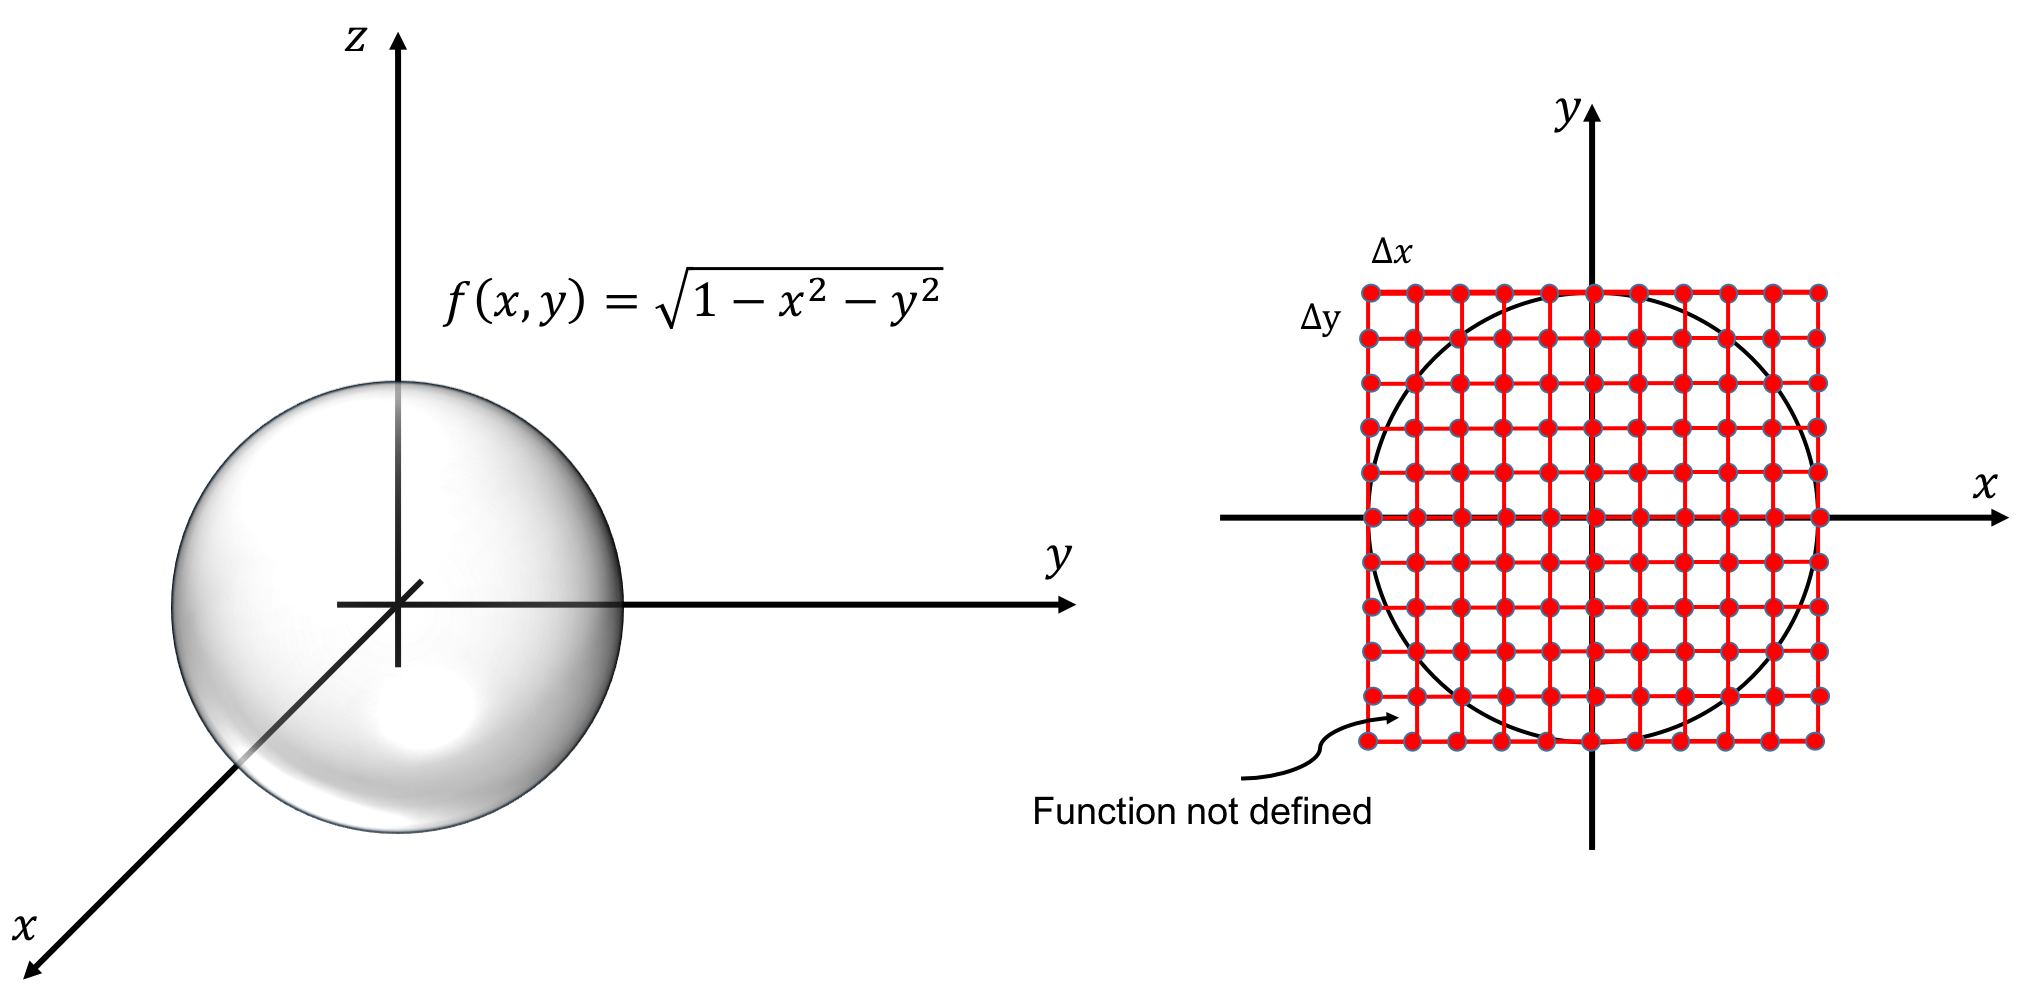
\includegraphics[width=1.0\linewidth]{fig-mc/2Dint.png}}
  \caption{
  Illustration of a 2D integration to evaluate the volume of a sphere.\label{fig:mc:2Dint}
  }
\end{figure}
%\clearpage % flush figures fig:mc:2Dint

The multi dimensional
integral is done by placing a box around the sphere, and divide this
box into $N\times N$ equal boxes. If start the integration
at $x=-R$, $F(-R)=0$, because the integrand is zero. If we move one
step to the left, we need to integrate from $y=-R$ to $y=R$. We see
from the figure to the right in figure~\ref{fig:mc:2Dint} that the
function is not defined for two first points. Thus we need to make
sure that if we are outside the integration bounds the function is
zero. Below is an implementation that uses recursive function calls


















\begin{lstlisting}[language=python,style=blue1]
def dd_trapez(lower_limit,upper_limit,func,x,i,N,D):
    h = (upper_limit-lower_limit)/N
    if(i == D-1):
        funci=d1_trapez
    else:
        funci=dd_trapez
    x[i]  = lower_limit
    area  = funci(lower_limit, upper_limit,func,x,i+1,N,D)
    x[i]  = upper_limit
    area += funci(lower_limit, upper_limit,func,x,i+1,N,D)
    area *= 0.5
    x[i]  = lower_limit
    for k in range(1,N): # loop over k=1,..,N-1
        x[i] += h # midpoint value
        area += funci(lower_limit, upper_limit,func,x,i+1,N,D)
    return area*h

\end{lstlisting}




\begin{graybox2admon}[Recursive functions]
\index{recursive functions}
Recursive implementation is very elegant, and more transparent, but it comes with a price. The reason is that when a function is called additional memory is allocated to store the local variables. If we where to calculate $100!$, 100 copies of the variable $n$ are created, whereas using a loop only one variable is created. Each time a function is called more memory is allocated, and if the recursive calls are too many it might cause memory overflow. If you try to call \Verb!fact_rec(1000)!, Python will give an error, because the maximum number of recursions are reached, it can be changed by:



\begin{lstlisting}[language=Python,style=gray]
import sys
sys.setrecursionlimit(1500)

\end{lstlisting}
\end{graybox2admon}






\begin{graybox2admon}[Error Analysis in higher dimensions]
In the chapter about numerical integration, we did an error analysis
on the trapezoidal rule and found that it scaled as $h^2$. As we see
from the example above, a higher order integration is simply to do a
series of 1D integrations in all the dimensions, thus the error term
should be $h_{x_0}^2+h_{x_1}^2+\cdots+h_{x_{d-1}}^2$. If we use the
same spatial resolution in all dimensions, then the overall error
scale as $h^2$. If we let $n$ denote the number of points in each
directions, $h\sim 1/n$, the total number of points used is $N=n\times
n\cdots n=n^d$. Thus, the error term scales as $h^2\sim N^{-2/d}$, and
we see that if $d\geq 4$, the MC integration is expected to perform
better.
\end{graybox2admon}




% --- begin exercise ---
\begin{doconceexercise}
\refstepcounter{doconceexercisecounter}

\exercisesection{Exercise \thedoconceexercisecounter: The central limit theorem}
                             
\label{ex:mc:norm}

\index{central limit theorem}
The central limit theorem is a corner stone in statistics, and it is
the reason for why the normal distribution is so widely used. The
central limit theorem states that if we calculate the average of an
independent random variable, the \emph{average will be distributed
according to a normal distribution}. Not that the central limit
theorem does not state anything about the distribution of the original
variable. We will not prove the central limit theorem, but illustrate
it with two examples. 

% !bsol
% !esol

% --- begin subexercise ---

\subex{a)}
First we will investigate a random variable that follows a \emph{uniform
distribution}. Write a Python function that returns the average of
$N$ uniformly distributed numbers in $[0,1]$.

% --- begin solution of exercise ---
\paragraph{Solution.}

















\begin{lstlisting}[language=python,style=blue1]
def average(N):
    x=[np.random.uniform() for _ in range(N)]
    return np.mean(x)

# or alternatively, and equally fast

def average2(N):
    x=0
    for i in range(N):
        x+=np.random.uniform()
    return x/N

# or much faster:
def average3(N):
    x=np.random.uniform(size=N)
    return np.mean(x)

\end{lstlisting}

% --- end solution of exercise ---

% --- end subexercise ---

% --- begin subexercise ---

\subex{b)}
Calculate the average $M$ times and make a histogram of the values.

% --- begin solution of exercise ---
\paragraph{Solution.}


\begin{lstlisting}[language=python,style=blue1]
def hist(M,N=100):

\end{lstlisting}

% --- end solution of exercise ---

% --- end subexercise ---

% --- begin subexercise ---

\subex{c)}
Repeat the above exercise for a Poisson distribution.

% --- begin solution of exercise ---
\paragraph{Solution.}













\begin{lstlisting}[language=python,style=blue1]
def average3(N):
    x=np.random.uniform(size=N)
    return np.mean(x)
    
def hist(M,N=100):
    y=[average3(N) for _ in range(M)]
    plt.hist(x=y, bins='auto', color='#0504aa',alpha=0.7, rwidth=0.85)
    plt.show()

def average4(N):
    x=[np.random.poisson() for _ in range(N)]
    return np.mean(x)

\end{lstlisting}

% --- end solution of exercise ---

% --- end subexercise ---

% Closing remarks for this Exercise

\paragraph{Remarks.}
It is quite remarkable that the distribution of the average values
from both a uniform and Poisson distribution follows a normal
distribution. The general
\href{{https://en.wikipedia.org/wiki/Central_limit_theorem}}{proof}\footnote{\texttt{https://en.wikipedia.org/wiki/Central\_limit\_theorem}}
is not that complicated, but the ramifications are large. The central
limit theorem explains why it makes sense to use the standard
deviation as a measure of confidence for the mean value.

\end{doconceexercise}
% --- end exercise ---

% --- begin exercise ---
\begin{doconceexercise}
\refstepcounter{doconceexercisecounter}

\exercisesection{Exercise \thedoconceexercisecounter: Birthday Paradox}
                             
\label{ex:mc:BP}

\index{birthday paradox}
The human mind is not good at logical thinking, and if we use our
intuition we often get into trouble. A well known example is the
''Birthday Paradox'', it is simply to answer the following question:
''How many randomly selected people do we need in order that there is
a 50\% chance that two of them have birthday on the same date?'' 

% !bsol
% !esol

% --- begin subexercise ---

\subex{a)}
Write a Python function that pick a random date
% subexercise...

% --- begin solution of exercise ---
\paragraph{Solution.}
Below are two examples, the first one picks a date, while the second
one just picks a random day at year.  
















\begin{lstlisting}[language=python,style=blue1]
#from datetime import date
#%%
import numpy as np

#def get_date():
#    """ return a random date in the current year """
#    start_dt = date.today().replace(day=1, month=1).toordinal()
#    end_dt = date.today().replace(day=31, month=12).toordinal()
#    random_day = date.fromordinal(np.random.randint(start_dt, end_dt))
#    return random_day


def get_day():
    """ return a random day in a year """
    return np.random.randint(1,365)

\end{lstlisting}

% --- end solution of exercise ---

% --- end subexercise ---

% --- begin subexercise ---

\subex{b)}
Write a function that takes as argument, number of persons in a group,
and returns 1 if two of them has birthday on the same date and 0
otherwise.

% --- begin solution of exercise ---
\paragraph{Solution.}
. 












\begin{lstlisting}[language=python,style=blue1]
def NoPeople(p):
    """ pick random dates in a year, return 1 if two
        is in the same date before p is reached """
    dates=[]
    for n in range(p):
        date=get_day()
        if date in dates:
            return 1
        else:
            dates.append(date)
    return 0

\end{lstlisting}

% --- end solution of exercise ---

% --- end subexercise ---

% --- begin subexercise ---

\subex{c)}
Write a function that returns the probability that two people in a
group of $p$ persons have birthday on the same day, and determine how
many people we need to have a probability of 50\%.

% --- begin solution of exercise ---
\paragraph{Solution.}
In order to get some statistics, we need to sample $N$ groups and
return the fraction of groups that had two persons with the same birthday.







\begin{lstlisting}[language=python,style=blue1]
def BP(p, N):
    prob=0.
    for i in range(N):
        prob += NoPeople(p)
    return prob/N
print(BP(200,1000))

\end{lstlisting}

By trial an error, we find that 23 persons is needed in order to have
a probability of
% --- end solution of exercise ---

% --- end subexercise ---

\end{doconceexercise}
% --- end exercise ---

% !split

\clearemptydoublepage
\markboth{Bibliography}{Bibliography}
\thispagestyle{empty}

\bibliographystyle{plain}
\bibliography{../chapters/papers}

% ------------------- end of main content ---------------

% #ifdef PREAMBLE
\cleardoublepage\phantomsection  % trick to get correct link to Index
\printindex

\end{document}
% #endif

